%% LyX 1.5.5 created this file.  For more info, see http://www.lyx.org/.
%% Do not edit unless you really know what you are doing.
\documentclass[12pt,twoside,english]{scrreprt}
\usepackage[T1]{fontenc}
\usepackage{fancyhdr}
\pagestyle{fancy}
\usepackage{array}
\usepackage{verbatim}
\usepackage{amsmath}
\usepackage{makeidx}
\makeindex
\usepackage[dvips]{graphicx}
\usepackage{amssymb}

\makeatletter

%%%%%%%%%%%%%%%%%%%%%%%%%%%%%% LyX specific LaTeX commands.
\newcommand{\noun}[1]{\textsc{#1}}
%% Because html converters don't know tabularnewline
\providecommand{\tabularnewline}{\\}

%%%%%%%%%%%%%%%%%%%%%%%%%%%%%% User specified LaTeX commands.
\usepackage{a4wide}
%% End LyX user specified preamble.
%\usepackage{fancybox}

\AtBeginDocument{
  \def\labelitemii{\(\circ\)}
  \def\labelitemiii{\normalfont\bfseries{--}}
}

\makeatother

\usepackage{babel}

\begin{document}

\title{EMPIRE \\
modular system for nuclear reaction calculations\\
{\Large (version: 2.19 Lodi)}}


\author{\textsf{M. Herman,} \textsf{\large P. Oblozinsky}, \textsf{}\\
\textsf{\normalsize NNDC, Brookhaven National Laboratory, Upton, USA}\\
\textsf{\normalsize e-mail: mwherman@bnl.gov}\textsf{}\\
\textsf{}\\
\textsf{\large R. Capote-Noy, A. Trkov, V. Zerkin,}{\large{} }\\
\textsf{\normalsize International Atomic Energy Agency, Vienna, Austria}\\
\\
\textsf{\large M. Sin,}{\large{} }\\
\textsf{\normalsize University of Bucharest, Bucharest, Rumania}\\
\\
\textsf{\large B.V. Carlson,}\\
\textsf{\normalsize ITA/Centro Tecnico Aeroespacial, Sao Jose dos
Campos, Brazil }\\
\textsf{\normalsize }\\
}

\maketitle
\begin{abstract}
EMPIRE is a modular system of nuclear reaction codes, comprising various
nuclear models, and designed for calculations over a broad range of
energies and incident particles. A projectile can be any nucleon or
Heavy Ion. The energy range starts just above the resonance region,
in the case of a neutron projectile, and extends up to few hundred
MeV for Heavy Ion induced reactions. The code accounts for the major
nuclear reaction mechanisms, such as optical model, Coupled Channels
and DWBA (ECIS03), Multi-step Direct (ORION + TRISTAN), NVWY Multi-step
Compound, exciton model (DEGAS) and the full featured Hauser-Feshbach
model. Heavy Ion fusion cross section can be calculated within the
simplified coupled channels approach (CCFUS). A comprehensive library
of input parameters covers nuclear masses, optical model parameters,
ground state deformations, discrete levels and decay schemes, level
densities, fission barriers (BARFIT), moments of inertia (MOMFIT),
and $\gamma$-ray strength functions. Effects of the dynamic deformation
of a fast rotating nucleus can be taken into account in the calculations.
The results can be converted into the ENDF-6 format using the accompanying
code EMPEND. The package contains the full EXFOR library of experimental
data. Relevant EXFOR entries in computational format C4 
are automatically retrieved during the
calculations. Plots comparing experimental results with calculations
can be produced 
%using X4TOC4 and PLOTC4 codes linked to the rest of
with ENDVER modules linked to the rest of
the system through bash-shell (UNIX) scripts. Publication quality
graphs can be obtained using the powerful and flexible plotting package
ZVView. The graphic user interface, written in Tcl/Tk, provides for
easy operation of the system. 
\end{abstract}
\newpage

~

\newpage

\tableofcontents{}

\newpage


\chapter{Introduction}

The first version of EMPIRE code was released in 1980. This code originally
contained the Hauser-Feshbach\index{Hauser-Feshbach} theory and the
classical HYBRID\index{HYBRID} model to account for the preequilibrium
effects. The width fluctuation correction was implemented in terms
of the HRTW approach \cite{HRTW,HHM}. Since that time, the code has
been continuously developed. Adding the FKK Multi-step Compound\index{MSC}
mechanism \cite{FKK} lead to the EMPIRE-MSC version. Subsequently,
the NVWY\index{NVWY} formulation of the Multi-step Compound mechanism
\cite{NVWY} was implemented in the HMS-EMPIRE. This version also
included combinatorial calculations of particle-hole level densities.
In addition, a version for Heavy Ion induced reactions (EMPIRE HI)
was developed.

EMPIRE-2 is a totally new release of the code. Contrary to the preceding
developments, which largely consisted in adding new features without
changing the structure of the code, the present version has been rewritten
from scratch, using different programming concepts. Taking advantage
of the relaxed memory limitations, all intermediate files were eliminated,
which together with careful coding of the most crucial parts of the
code, increased the speed of the program by a factor of 20. The new
code is projected to be general and flexible, and can been applied
to the calculation of neutron capture in the keV region, as well as
for Heavy Ion (HI) induced reactions at several hundreds of MeV. All
dimensions in the main code are set up through the parameter statements
contained in the separate file, which is included wherever appropriate,
making any adjustment of the code to the actual problem and/or computer
straightforward. The code has a modular structure. Each module performs
a well defined task and communicates with other modules through a
set of global COMMONS which are included in most of the subroutines.
This assures access to all the resources throughout the code, and
facilitates adding new features and mechanisms.

EMPIRE makes use of several codes, written by different authors, which
 were converted into subroutines and adapted for the present use.
In most cases, the modifications concerned input/output interface
and never affected the physical model contained in the original source.
The following codes are incorporated in the present version of EMPIRE:

\begin{labeling}{MMMMMMMMMMM}
\item [{\textbf{ECIS03\index{ECIS}}}] Coupled-Channels\index{Coupled-Channels}
and DWBA\index{DWBA} code by J. Raynal~\cite{ECIS},
\item [{\textbf{CCFUS\index{CCFUS}}}] simplified Coupled-Channels calculation
of HI fusion cross section by C.H. Dasso and S. Landowne~\cite{CCFUS},
\item [{\textbf{ORION\index{ORION}~\&~TRISTAN\index{TRISTAN}}}] TUL\index{TUL}~\cite{TUL}
approach to Multi-step Direct\index{MSD} by H. Lenske~\cite{ORTRI},
\item [{\textbf{DEGAS\index{DEGAS}}}] exciton model with angular momentum
conservation and $\gamma$ emission~\cite{Degas} by E. B\v et\' ak
and P. Oblo\v zinsk\' y,
\item [{\textbf{DDHMS\index{DDHMS}}}] Monte Carlo simulation of the preequilibrium
decay by M.B. Chadwick~\cite{DDHMScode}
\item [{\textbf{BARMOM\index{BARMOM}}}] fission barriers and moments of
inertia by A. Sierk~\cite{sierk}.
\end{labeling}
The reader is referred to the original papers for a more detailed
description of these incorporated codes. Furthermore, the package
includes the following stand-alone codes:

\begin{labeling}{MMMMMM}
\item [{\textbf{EMPEND\index{EMPEND}}}] converts EMPIRE results into ENDF-6
format (written by A. Trkov),
\item [{\textbf{ENDRES\index{ENDRES}}}] merges existing resonance parameters
into ENDF-6 formatted file produced by EMPEND (written by A. Trkov),
\item [{\textbf{X4TOC4\index{X4TOC4}}}] converts experimental data retrieved
from EXFOR into computational C4 format (written by D.E. Cullen)~\cite{PREPRO},
\item [{\textbf{C4SORT\index{C4SORT}}}] sorts experimental data in the
computational C4 format file by MAT/MF/MT numbers and incident energy
(written by A.Trkov)~\cite{ENDVER},
\item [{\textbf{FIXUP\index{FIXUP}}}] used to reconstruct redundant cross sections
MT=4, 103, and 107 (Program of the Pre-Pro series, written by D.E. Cullen)~\cite{PREPRO},
\item [{\textbf{LEGEND\index{LEGEND}}}] reconstructs tabular linearly interpolable
angular distributions from ENDF data in different format representations 
(Program of the Pre-Pro series, written by D.E. Cullen)~\cite{PREPRO},
\item [{\textbf{LSTTAB\index{LSTTAB}}}] tabulates ENDF and EXFOR data
in PLOTTAB format (module of ENDVER package, written by A.Trkov)~\cite{ENDVER},
\item [{\textbf{SIXTAB\index{SIXTAB}}}] converts ENDF file MF6 to Law
7 representation (module of ENDVER package, written by A.Trkov)~\cite{ENDVER},
\item [{\textbf{PLOTC4\index{PLOTC4}}}] plots comparison between EMPIRE
results and EXFOR data (written by D.E. Cullen and A. Trkov)~\cite{ENDVER},
\item [{\textbf{CHECKR\index{CHECKR}}}] performs format checking of the
ENDF-6 formatted file (ENDF Utility codes, written by Ch. Dunford)
\item [{\textbf{FIZCON}}] performs physics check of the ENDF-6 formatted
file (ENDF Utility codes, written by Ch. Dunford)
\item [{\textbf{PSYCHE}}] performs more physics checking of the ENDF-6
formatted file (ENDF Utility codes, written by Ch. Dunford)
\item [{\textbf{LINEAR}}] converts MF=3 (cross sections) in an ENDF
file into a linear-linear interpolable form (Program of the Pre-Pro series, 
written by D.E. Cullen)~\cite{PREPRO}
\item [{\textbf{PLTLST}}] prepares a list of data types in the EXFOR data-base
that can be compared to quantities in the ENDF files
(module of ENDVER package, written by A.Trkov)~\cite{ENDVER},
\item [{\textbf{RECENT}}] reconstructs the resonace contribution to the
cross sections in an ENDF file into linearly interpolable form 
(Program of the Pre-Pro series, written by D.E. Cullen)~\cite{PREPRO}
\item [{\textbf{SIGMA1}}] Doppler broadens neutron induced cross sections
in an ENDF file
(Program of the Pre-Pro series, written by D.E. Cullen)~\cite{PREPRO}
\item [{\textbf{STANEF}}] Standardizes ENDF-6 formatted file
(ENDF Utility codes, written by Ch. Dunford)
\item [{\textbf{zvvddx}}] Produces plots of angular distributions, spectra
and double differential cross sections using ZVView package (written
by V. Zerkin).
\item [{\textbf{c4zvd}}] ZVView\textbf{\index{ZVView}} plotting package
by V. Zerkin~\cite{ZVView}.
\end{labeling}
The next chapter outlines nuclear reaction models used in the code.
Both, the structure of the code and the input/output files are described
in Chapter~\ref{Chap:code}. Use of the code, the role of input parameters,
and a few typical examples of input files are discussed in Chapter~\ref{Chap:work}.


\chapter{Models}


\section{Fusion/reaction cross section\label{sec: fusion}}

The reaction cross section is calculated in terms of transmission
coefficients $T_{l}^{a}(\epsilon)$ using the expression

\begin{equation}
\sigma_{a}(U,J,\pi)=\frac{\pi}{k^{2}}\frac{(2J+1)}{(2I+1)(2i+1)}\sum_{S=|I-i|}^{I+i}\sum_{l=|J-S|}^{J+S}f(l,\pi)T_{l}^{a}(\epsilon),\label{fusion}\end{equation}


\noindent where $k$ is the wave number of relative motion, $i,I,J,$
and $S$ indicate projectile, target, compound nucleus, and channel
spin, respectively, and $l$ is the orbital angular momentum of the
projectile $a$. The function $f(l,\pi)$ ensures parity conservation.
It is unity if $p*P*(-1)^{l}=\pi$ and zero otherwise. Here $p,\, P,$
and $\pi$ are projectile, target, and compound nucleus parities and
$\epsilon$ and $U$ stand for the projectile and compound nucleus
energy. 

For projectiles with mass numbers A<5 the transmission coefficients
entering Eq.~\ref{fusion} are calculated using optical model routine
ECIS03\cite{ECIS} unless an external file FUSION exists. In the latter
case, the spin distribution of the Compound Nucleus is constructed
from this file.

The Heavy Ion fusion cross section is calculated using Eq. \ref{fusion}
with transmission coefficients determined according to one of the
following methods:

\begin{labeling}{00.00.0000}
\item [{(i)}] Simplified Coupled-Channels\index{Coupled-Channels}
approach \cite{CCFUS} (CCFUS\index{CCFUS} code). Inelastic excitations
and transfer reaction channels are treated as independent modes which
couple to the initial ground state. The corresponding wave equations
are approximately uncoupled by diagonalizing the interaction at the
barrier. The total transmission probability is then obtained by summing
over the distribution of transmission probabilities for the eigenbarriers,
with weights given by the overlap of the initial state with the eigenchannels.
This is a default option. It takes into account coupling of the excited
collective states in the target and projectile. A detailed description
of the method can be found in the original reference \cite{CCFUS}.
\item [{(ii)}] Distributed fusion-barrier\index{distributed fusion-barrier}
model \cite{difusb}. This method accounts for the effective lowering
of the one-dimensional fusion barrier by allowing for the additional
dimension and assuming that the barrier distribution in the added
dimension can be represented by a truncated Gaussian. Thus the fusion
barrier distribution $f(B')$ can be characterized by the mean energy
$B$, the standard deviation $\sigma_{B}$, and the truncation parameter
$t$, and is written as \begin{equation}
f(B')=n_{0}\exp\left(\frac{B-B'}{2\sigma_{B}^{2}}\right)^{2}\label{distbarr}\end{equation}
for $\left|B-B'\right|<t\sigma_{B}$ and $f(B')=0$ otherwise. The
parameter $t$ defines the lowest possible value of the fusion barrier
and $n_{0}$ is the normalization factor ensuring that the integral
of Eq. \ref{distbarr} is 1. The fusion probability for a given angular
momentum $l$ is given by a convolution of the barrier distribution
$f(B')$ and the transmission coefficient $T_{l}(E-B')$ \begin{equation}
p(E,l)=\int_{-\infty}^{\infty}f(B')T_{l}(E-B')dB'\,.\end{equation}
 The transmission coefficient in the Hill-Wheeler\index{Hill-Wheeler}
approach \cite{HillWheeler} reads\begin{equation}
T_{l}(E-B')=\left\{ 1+\exp\left[-2\pi(E-B'-E_{rot})/(\hbar\omega)\right]\right\} ^{-1}\,,\end{equation}
with $E_{rot}$ being rotation energy at angular momentum $l$. The
distributed fusion-barrier\index{distributed fusion-barrier} option
in EMPIRE allows for the extra-push energy that can be specified in
the input and added to the fusion barrier. The latter, if not specified
in the input, is by default calculated using BAR subroutine of CCFUS\index{CCFUS}
(see above) .
\item [{(iii)}] Fusion cross sections for each $l$ read from the external
file \emph{FUSION} (\emph{{*}.fus}). The code converts them into transmission
coefficients to be used in Eq.\ref{fusion}. The existence of the
\emph{FUSION} (\emph{{*}.fus}) file overrides all input dispositions
regarding fusion determination.\\
NOTE: \emph{FUSION} (\emph{{*}.fus}) file refers to a single incident
energy, therefore only one energy at a time can be calculated.
\end{labeling}
%
\begin{comment}
(iv) Bass approach\cite{Bass} with nucleus-nucleus potential taken
from\cite{Basspot}. Let us define \begin{equation}
R_{12}=R_{1}+R_{2}=1.16A_{1}^{1/3}-\frac{1.39}{A_{1}^{1/3}}+1.16A_{2}^{1/3}-\frac{1.39}{A_{2}^{1/3}},\label{r12}\end{equation}
 two dimensionless parameters\begin{equation}
x=\frac{e^{2}}{r_{0}a_{s}}\frac{Z_{1}Z_{2}}{A_{1}^{1/3}A_{2}^{1/3}(A_{1}^{1/3}+A_{2}^{1/3})^{2}},\label{xbass}\end{equation}
\begin{equation}
y=\frac{\hbar^{2}}{2m_{0}r_{^{2}0}a_{s}}\frac{A_{1}+A_{2}}{A_{1}^{1/3}A_{2}^{1/3}(A_{1}^{1/3}+A_{2}^{1/3})^{2}},\label{ybass}\end{equation}
and\begin{equation}
f=\left\{ 1+\frac{2}{5}\left(\frac{m_{1}R_{1}^{2}}{\mu R_{12}^{2}}+\frac{m_{2}R_{2}^{2}}{\mu R_{12}^{2}}\right)\right\} ^{-1},\label{fbass}\end{equation}
where $\mu=m_{0}A_{1}A_{2}/\left(A_{1}+A_{2}\right)$, $a_{s}$ is
the surface term in the liquid drop model mass formula, and indexes
\emph{1} and \emph{2} refer to projectile and target respectively.
According to Bass the critical (limiting) angular momentum for fusion
is\begin{equation}
l_{cr}(E_{1})=\left\{ \frac{1-x}{2y}\right\} ^{1/2}\label{le1bass}\end{equation}
at bombarding energies below $E_{1}$given by\begin{equation}
E_{1}=\frac{Z_{1}Z_{2}e^{2}}{R_{12}}\left\{ 1+\frac{1-x}{2x}-\frac{1}{x}\frac{d}{R_{12}}\right\} \label{e1bass}\end{equation}
and \begin{equation}
l_{cr}(E_{2})=\frac{1}{f}\left\{ \frac{1-x}{2y}\right\} ^{1/2}\label{le2bass}\end{equation}
for incident energies between $E_{1}$ and $E_{2}$\begin{equation}
E_{2}=\frac{Z_{1}Z_{2}e^{2}}{R_{12}}\left\{ 1+\frac{1}{f^{2}}\frac{1-x}{2x}-\frac{1}{x}\frac{d}{R_{12}}\right\} \label{e2bass}\end{equation}

\end{comment}
{}

\begin{labeling}{00.00.0000}
\item [{(iv)}] Total fusion cross section specified in input (single
incident energy only).
\item [{(v)}] Critical angular momentum $l_{cr}$ for compound nucleus
formation specified in input (single incident energy only).
\end{labeling}
In the latter two cases the transmission coefficients are assumed
to be of the form

\begin{equation}
T_{l}^{a}(\epsilon)=\frac{1}{1+exp(-\frac{l_{cr}-l}{\delta l})}\,,\label{Tlfus}\end{equation}


\noindent where $\delta l$ is an input parameter. If the total fusion
cross section is specified in the input, then the code adjusts $l_{cr}$
in order to reproduce the requested value. 


\section{Coupled-Channels\index{Coupled-Channels} Code ECIS\index{ECIS}}

ECIS \cite{ECIS} is a well known and highly respected code for calculations
within the generalized optical model and Coupled-Channels model (CC).
These are important for modeling reactions on deformed nuclei and,
in particular, for the correct description of a strong population
of collective discrete levels in the inelastic scattering. ECIS-95
was added to EMPIRE as its new extensive module by R. Capote in February
2001 and replaced with the ECIS03 version in EMPIRE-2.19. Symmetric
rotational, vibrational-rotational and harmonic-vibrational CC modes
are available. The implementation features automatic preparation of
the ECIS03 input. It uses the RIPL\index{RIPL}-2 \cite{RIPL} optical
model segment and resorts to the RIPL-2 discrete level schemes and
to the deformation parameters (quadrupole deformations $\beta_{2}$)
only if these are not included in the optical model parameter set
available from RIPL-2. Since EMPIRE has no table of vibrational (dynamical)
deformations, these are defined in a somewhat ad hoc manner as 0.15
for quadrupole and 0.05 for octupole vibrations. 

Calculations can be performed for the majority of deformed nuclei
including rotational and vibrational, even-even and even-A with integer
spins, as well as odd-A with half-integer spins. Vibrational even-even
nuclei and even-A are also covered. The only exceptions are vibrational
odd-A nuclei. In these cases automatic construction of the file with
collective levels is not possible and the user must prepare the corresponding
file manually.

Once ECIS03\index{ECIS} is invoked, the code prepares several interim
files to be read by EMPIRE. In most cases, the code prepares two additional
files:

\begin{labeling}{MMMMMMMMMMM}
\item [{TARGET\_COLL.DAT,}] collective levels and their deformations to
be used by the rotational or vibrational CC. In the case of vibrational
model the phonon structure of the levels is also read from this file
(in the case of the rotational model this information is ignored).
\item [{OMPAR.DIR,}] parameters of the Optical Model Potential (OMP) to
be used in the inelastic channel (discrete collective levels). OMP
parameters may be selected via a new keyword DIRPOT (similar to OMPOT,
but only for the inelastic channel). This information is supplemented
by the parameters read from the \emph{{*}-lev.col} file.
\end{labeling}
ECIS03\index{ECIS} can be invoked by the EMPIRE in three different
ways, using input directive DIRECT. The default value (DIRECT=0) calls
the spherical optical model and suppresses calculation of direct reactions
to the discrete levels. The remaining options have the following meaning:

\begin{labeling}{MMMMMMM}
\item [{DIRECT~1.}] Population of discrete, collective levels in the inelastic
scattering is calculated using the Coupled-Channels\index{Coupled-Channels}
model. The direct cross sections are exact but spherical transmission
coefficients $T_{l}$ are used for subsequent preequilibrium and HF\index{Hauser-Feshbach}
calculations in the whole energy grid. These results are re-normalized
at the $T_{l}$ level by taking into account direct component. The
total, elastic, absorption and the inelastic cross sections are taken
from the CC calculations if a true Coupled-Channel Optical Model Potential
(CC-OMP) is being used (otherwise, in the case of the Spherical OMP
(S-OMP), only inelastic cross sections are accepted). \\
The option DIRECT=1 is fairly fast, though some accuracy may be lost
compared to the DIRECT=2 option described below. In general, it should
perform well for the weakly coupled levels. For strong coupling, such
as in the highly deformed rotational bands in heavy nuclei, it should
be used with caution. It is the recommended option if accuracy is
not a critical issue and the appropriate CC-OMP is available.
\item [{DIRECT~2.}] Population of discrete, collective levels in the inelastic
scattering is calculated within the CC as above. Importantly, the
CC is used consistently, considering the ground state and the coupled
levels, to calculate all necessary transmission coefficients for subsequent
preequilibrium and HF\index{Hauser-Feshbach} calculations. These
CC transmission coefficients define absorption cross section that
is available for the preequilibrium and HF decay. The absorption cross
section sums up with the direct cross sections to collective levels
to the reaction cross section. DIRECT=2 is an exact option that considers
flux decrease due to the collective excitations at the level of $T_{l}$.
In the first run with DIRECT=2, $T_{l}$ values are calculated for
the whole energy grid. These values are stored in the file \emph{{*}.tl}
for further use. Although the first run takes quite a lot of time,
all successive runs are much faster. It should be noted that file
\emph{{*}.tl} can be used for successive runs only if no changes were
made to the files \emph{{*}-lev.col} and \emph{{*}-omp.ripl}. For
each incident energy in the input file, there is one \emph{{*}.tl}
file stored in the \emph{work} directory. The DIRECT=2 is a recommended
option for accurate calculations whenever an appropriate CC-OMP is
available.
\item [{DIRECT~3.}] Population of discrete collective levels in the inelastic
scattering is calculated using the DWBA\index{DWBA} method providing
approximate direct cross sections. The spherical transmission coefficients
$T_{l}$ are used for the whole energy grid in subsequent preequilibrium
and HF\index{Hauser-Feshbach} calculations. These results are re-normalized
at the $T_{l}$ level by taking into account direct component. \\
This option is fairly fast, though some accuracy may be lost. In general,
it should perform well for weakly coupled levels. For a strong coupling,
such as in the highly deformed rotational bands in heavy nuclei, it
should be used with caution. The DWBA\index{DWBA} option has an advantage
if the suitable CC-OMP is not available. In such a case, one can use
S-OMP parameters in the DWBA calculations tuning inelastic cross sections
by adjusting dynamical deformations of collective levels in file \emph{{*}-lev.col}
.
\end{labeling}

\section{Multi-step Direct}

The approach to statistical Multi-step Direct\index{MSD} reactions
is based on the Multi-step Direct (MSD) theory of preequilibrium scattering
to the continuum originally proposed by Tamura, Udagawa and Lenske
\cite{TUL}. Since then, the approach has been revised, especially
the part related to statistical and dynamical treatment of nuclear
structure. 

The evolution of the projectile-target system from small to large
energy losses in the open channel space is described in the MSD theory
with a combination of direct reaction (DR), microscopic nuclear structure
and statistical methods. As typical for the DR-approach, it is assumed
that the closed channel space, i.e. the MSC\index{MSC} contributions,
have been projected out and can be treated separately within the Multi-step
Compound\index{MSC} mechanism.


\subsection{\label{sec: MSD}Outline of the theory}

In the MSD\index{MSD} theory the effective Hamiltonian in the open
channel space is divided into an energy averaged optical model part
$H^{opt}$, describing the relative motion of projectile $a$ and
target $A$, the intrinsic Hamiltonian $H^{intr}$ of the asymptotically
separated nuclei and the residual effective projectile-target interaction
$V^{res}$ leading to non-elastic processes

\begin{equation}
H=H^{opt}+H^{intr}+V^{res}\quad.\label{fullh}\end{equation}
Both $H^{opt}$ and $V^{res}$ are non-hermitian operators. To a large
extent the imaginary parts are related to the flux absorbed into the
closed channels, but those open channels which are not treated explicitly
are also contributing. 

The ORION\index{ORION} code solves the Lippmann-Schwinger equation
for the open channel T-matrix where the $n^{th}$-order term

\begin{equation}
T_{\gamma0}^{(n)}=<\chi_{E}^{(-)}|(\gamma|V^{res}(G^{chan}(E)V^{res})^{n-1}|0)|\chi_{0}^{(+)}>\label{tgamman}\end{equation}
describes the $n-$step transition from the entrance channel with
incoming scattering wave $\chi_{0}^{(+)}$ and the ground state configuration
$|0)=|aA)$ to an exit channel $\gamma$ with outgoing wave $\chi_{E}^{(-)}$
at the energy E \cite{SLW,LW92}. $G^{chan}(E)$ is the Green's function
for the channel. The scattering waves are optical model wave functions.
They are weakly energy dependent on a scale much larger than the one
on which the intrinsic states $\gamma$ vary. The MSD\index{MSD}
approach treats the residual projectile-target interactions perturbatively.
In this sense, MSD theory is a {}``weak coupling'' description of
continuum scattering.

In order to describe the statistical content of pre-equilibrium spectra
the real states $\gamma$ are expanded into \emph{n}-particle and
\emph{n}-hole model states $c$. Explicitly, $H^{intr}$ is chosen
as \begin{equation}
H^{intr}=H_{0}^{intr}+V^{intr}\quad.\label{hintr}\end{equation}
 The states $c$ are eigenstates of $H_{0}^{intr}$ and the residual
interaction $V^{intr}$ couples states from different particle-hole
classes only. It is assumed that the configuration mixing between
$np-nh$ classes is stochastic in nature and leads to a random distribution
of amplitudes with mean value zero \cite{LW92}. When the density
matrix is averaged over a finite energy interval, e.g. with a Lorentzian
or Gaussian $g(x)$ of full width $\Delta$ large compared to the
mean level spacing, \begin{equation}
\hat{\rho}(E)=\int dE'g(E-E')\hat{\rho}_{micro}(E)\label{rhoav}\end{equation}
the coherence of the basis states is lost. As a result, the density
matrix becomes a statistical matrix \begin{equation}
\hat{\rho}(E)=\sum_{n}{\hat{\rho}_{n}(E)}.\label{levelc}\end{equation}
The summation extends over the $np-nh$ classes with \begin{equation}
\hat{\rho}_{n}(E)=\sum_{c=[npnh]}{|c)P_{c}(E)(c|}\label{leveld}\end{equation}
and the probability per energy to find the system in the configuration
$c$ is given by the spectroscopic densities,

\begin{equation}
P_{c}(E)=-\frac{1}{\pi}Im[\int dE'g(E-E')(c|G^{intr}(E')|c)]\,,\label{specd}\end{equation}
with $G^{intr}(E)$ being the intrinsic Green's function.

The statistical operators carry further properties which are important
for the physical content of the description. Integrating $P_{c}(E)$
over an interval $\Delta E$ one obtains the spectroscopic factor
for the configuration $c$ in $\Delta E$. Irrespective of the representation,
i.e. in either the $\gamma$ or the $c$ basis, the trace of $\hat{\rho}(E)$,
Eq. \ref{rhoav}, gives the total level density\index{level density}
at energy $E$. The partial level density of $np-nh$ states is determined
by $tr(\hat{\rho}_{n})$ (Eq. \ref{leveld}). 

Similar to the chaining and never-come-back hypotheses of \cite{FKK}
the interference terms $n\ne k$ are neglected by assuming that in
each step the reaction is dominated by transitions into configurations
with the highest level density at a given excitation energy. This
means, that we neglect de-excitation and re-scattering processes which
decrease or leave the $ph-$number unchanged, respectively. With this
assumption the cross section becomes an incoherent super-position
of $n-$step contributions

\begin{equation}
\frac{d^{2}\sigma}{d\Omega dE}=\sum_{n}{\frac{d^{2}\sigma^{(n)}}{d\Omega dE}}\,,\label{sigma0}\end{equation}
where the multi-step cross sections are defined as \begin{equation}
\frac{d^{2}\sigma^{(n)}}{d\Omega dE}=\sum_{c=[npnh]}{P_{c}(E)|T_{c0}^{(n)}|^{2}}\,.\label{sign}\end{equation}
 Expanding $V^{res}$ into multi-poles $V_{\lambda}$ and noting that
only $1p-1h$ configurations are directly excited in a one-step process
the $\sigma^{(1)}$ is determined by an average over transitions into
the $1p-1h$ states $c$ around excitation energy $E$ with form factors
\begin{equation}
F_{\lambda}^{c0}=(c|V_{\lambda}|0)\,.\end{equation}
Rather than treating each transition separately it is sufficient to
consider averages over the microscopic form factors. Thus, $V^{res}$
is represented in terms of state independent multipole form factors
$F_{\lambda}$ and nuclear transition operators $O_{\lambda}$ \begin{equation}
V^{res}(r,\xi)=\sum_{\lambda}{F_{\lambda}(r)O_{\lambda}(\xi)}.\label{vres}\end{equation}
Here, $r$ denotes the relative motion coordinate and $\xi=(\xi_{a},\xi_{A})$
are the intrinsic coordinates including spin and isospin, respectively.
The multipole form factors $F_{\lambda}$ in turn are related to $O_{\lambda}$.
In a self-consistent approach they are obtained by averaging $V^{res}$
over $O_{\lambda}$: \begin{equation}
F_{\lambda}(r)=(c|O_{\lambda}^{\dag}\hat{\rho}(E)V^{res}|c)/S_{\lambda}(E,c).\label{formf}\end{equation}
Here, the general case of a transition starting from an arbitrary
state $c$ is considered which appears in the intermediate steps of
higher order multi-step processes. For one-step reactions the initial
state is the ground state $c=0$. By normalization to the transition
strength function $S_{\lambda}$\begin{equation}
(c|O_{\lambda'}^{\dag}\hat{\rho}(E)O_{\lambda}|c)=\delta_{\lambda\lambda'}S_{\lambda}(E,c)\label{slambda}\end{equation}
the dependence of the form factor on the internal state is removed
to a large extent. $S_{\lambda}$ is the nuclear response function
for the external operator $O_{\lambda}$ describing the transition
rate per unit energy from the state $c$ into the ensemble of states
$c'$ centered at energy $E$.

The above relations are appropriate for one-step reactions where $c$
is the ground state. However, in higher steps $c$ is an arbitrary
intermediate $np-nh$ state which is summed over in the cross section.
Thus, for multi-step scattering the form factor, Eq.\ref{formf} actually
utilizes a too microscopic picture. The statistical aspects in multi-step
transitions are taken fully into account by the average multipole
form factors \begin{equation}
F_{\lambda}=\frac{tr(\hat{\rho}O_{\lambda}^{\dag}\hat{\rho}V^{res})}{tr(\hat{\rho}O_{\lambda}^{\dag}\hat{\rho}O_{\lambda})}\,,\label{fav}\end{equation}
which are independent of the initial state and the multi-step order,
respectively. In the applications of the theory these global form
factors together with the response functions of Eq.\ref{slambda}
are used.

With the above results the one-step cross section is expressed as
\begin{equation}
\frac{d^{2}\sigma^{(1)}}{dEd\Omega}=\sum_{\lambda}{S_{\lambda}(E)\overline{\frac{d\sigma^{(1)}}{d\Omega}}\mid_{\lambda}}\,,\label{sigma1}\end{equation}
where $\overline{\sigma^{(1)}}$ is a reduced DWBA\index{DWBA} cross
section calculated with the average form factors (Eq.\ref{formf}).

The multi-step part of the theory is discussed here for two-step reactions
only. The state-independent and slowly varying two-step amplitudes
read\begin{equation}
T_{\lambda_{1},\lambda_{2}}^{(2)}=<\chi_{E}^{(-)}|F_{\lambda_{2}}G^{opt}F_{\lambda_{1}}|\chi_{\alpha}^{(+)}>\,,\label{amp2}\end{equation}
with $G^{opt}$ being Green's function for the optical model potential.
The nuclear structure information is now contained completely in \begin{equation}
(0|O_{\lambda'_{1}}^{\dag}G^{(intr)\dag}(E'_{1})O_{\lambda'_{2}}^{\dag}\hat{\rho}(E)O_{\lambda_{2}}G^{(intr)}(E_{1})O_{\lambda_{1}}|0)\,.\label{two1}\end{equation}
By definition, the exit channel configurations are $2p-2h$ states
which are excited from $1p-1h$ states $c_{1}$. Also in the first
step only $1p-1h$ states $a$ are excited. Therefore, we only have
to consider the $1p-1h$ reduced parts of the two Green functions. 

To a good approximation the dependence of $S_{\lambda_{2}}(E,c_{1})$
on $c_{1}$ can be replaced by a dependence on $E_{1}$ by considering
that the spectroscopic strength usually is located in the vicinity
of the unperturbed energy. Theoretically, this is achieved by taking
the average over the response functions belonging to states $c_{1}$
at energy $E_{1}$\begin{eqnarray}
S_{\lambda}(E,E_{1}) & = & \frac{\sum_{c_{1}}{P_{c_{1}}(E_{1})S_{\lambda}(E,c_{1})}}{\sum_{c_{1}}{P_{c_{1}}(E_{1})}}\nonumber \\
 & = & \frac{tr(\hat{\rho}_{1}(E_{1})O_{\lambda}^{\dag}\hat{\rho}(E)O_{\lambda})}{tr(\hat{\rho}_{1}(E_{1}))}\quad.\label{slave}\end{eqnarray}
The final result for the two-step MSD\index{MSD} cross section is
of very intuitive structure \begin{equation}
{d^{2}\sigma^{(2)}}/{dEd\Omega}=\sum_{\lambda_{1}\lambda_{2}}{\int dE_{1}S_{\lambda_{2}}(E,E_{1})S_{\lambda_{1}}(E_{1},0)\overline{\frac{d\sigma^{(2)}}{d\Omega}}(E,E_{1})\mid_{\lambda_{1}\lambda_{2}}}.\label{sigma2}\end{equation}
$\overline{\sigma^{(2)}}$ is an averaged cross section defined in
terms of the $T^{(2)}-$matrix elements (Eq.\ref{amp2}, which describes
two-step scattering wave-mechanically as a coherent quantal process.
The total response of the intrinsic system at energy loss $E$ is
contained in the first and second step transition strength functions.
The folding accounts for the partitions of the total energy $E$ into
one- and two-step parts such that $E$ is conserved. 

In the present version of the code only one- and two-step MSD\index{MSD}
contributions are considered. In most cases it is a good approximation
to use the ground state response functions also for the second step
but at an energy shifted by the amount of total energy loss in the
first step. This corresponds to the assumption that the structure
of excited nuclei is close to the structure of the ground state as
far as single particle occupancies and other mean-field properties
are concerned. 

Summarizing this section, the statistical properties of pre-equilibrium
spectra are used to eliminate interference contributions at various
places. Physically, this corresponds to the neglect of certain intrinsic
correlation functions which only would be observable at an energy
resolution of the order of the average level spacing. This leads to
a representation of pre-equilibrium cross sections as an incoherent
super-position of multi-step contributions. The statistical treatment
is introduced in a minimal way, namely referring only to the intrinsic
systems while multi-step scattering is described quantum-mechanically
as a coherent process at all steps.


\subsection{Notes on RPA-Description of Transition Strength Functions}

In the MSD\index{MSD} approach continuum scattering is considered
as a sequence of $1p-1h$ transitions and the transition strength
functions, Eq. \ref{slambda}, correspond to response functions of
an external one-body operator acting repeatedly on a nucleus. A reliable
description of one-body response functions is provided by the Random
Phase Approximation theory \cite{Neg,Wal} (RPA\index{RPA}). In RPA
the whole series of $1p-1h$ interaction diagrams is summed exactly.
Thus, an essential contribution to the intrinsic correlations is treated
explicitly. In the notation of Section \ref{sec: MSD} they are part
of $H_{0}^{intr}$. Thus, the $ph-$classes are built from correlated
basis states. This justifies also the \textit{ansatz} of Eq. \ref{hintr}
where $V^{intr}$ was defined as to act only between $ph-$classes.

An important advantage for a reliable description of pre-equilibrium
spectra is that RPA\index{RPA} accounts for collective and non-collective
features on the same theoretical footing \cite{Wal,BM,LW92,SLW,RegT}.
The approach describes at the same time the large amount of weakly
excited background states and the strongly excited giant resonances
$(GR)$ in the continuum together with low-lying surface vibrations.
It is clear that the response functions do not suffer from double
counting of transition strength which appears if collective states
are treated separately. Important quantities like energy weighted
sum rules are known to be conserved by RPA\index{RPA}. Also the enhancement
of the response due to ground state correlations is included.

In view of a large number of $p-h$ configurations which are needed
in order to describe nuclear spectra over a range of excitation energies
of several tens of $MeV$ a fully microscopic calculation is of little
use. In accordance with the statistical description of cross section
statistical considerations are also incorporated into the structure
calculations. Instead of solving the RPA\index{RPA}-eigenvalue problem
by direct diagonalization it is more appropriate to consider the average
properties of excitations. The Green function approach to RPA\index{RPA}
\cite{Wal,LW92} provides the proper theoretical basis for such a
description.

For a general formulation, applicable also to open shell nuclei, the
quasi-particle RPA (QRPA) is used. Thus, a BCS\index{BCS} ground
state and a canonical transformation to quasi-particles is assumed
\cite{RS}. The excitations are then given in terms of two quasi-particle
($2qp$) rather than by $1p-1h$ configurations. Furthermore, in order
to account for the self-energies the $2qp$ energies are taken to
be complex by adding a state dependent damping width $\Gamma_{\alpha}^{\downarrow}$.
The response functions include inelastic events only and are calculated
in linear response theory. Formally, the response functions entering
into the MSD\index{MSD}-calculation are expressed through the RPA
polarization propagator $\chi^{RPA}(E)$

\begin{equation}
S_{\lambda}(E,0)=-\frac{1}{\pi}Im[\chi^{RPA}(E)]\,.\label{sgrpa}\end{equation}
In higher steps, where the transition starts from a state $c\not=0$,
the $1p1h$ densities and response functions on the background of
an already excited nucleus are required. At excitation energies per
particle which are well below the Fermi energy the structure remains
close to the ground state. Since this is the region of main interest
for pre-equilibrium scattering Eq.\ref{sgrpa} is used also in two-step
and higher order reactions at the appropriate excitation energy. The
average response functions, Eq.\ref{slave}, are approximated by

\begin{equation}
S_{\lambda}(E,E_{1})\simeq S_{\lambda}(E-E_{1},0)\,,\label{slrpa}\end{equation}
where it is assumed that $S_{\lambda}$ depends only on energy difference
$E-E_{1}$ which corresponds to the relative excitation energy. The
form factors of Eq.\ref{fav} are found to be given by folding $V^{res}$
with $\overline{\rho_{\lambda}}$. Thus, the theory leads to a transparent
and consistent description of nuclear structure and reaction dynamics
which accounts for the microscopic and the statistical aspects of
pre-equilibrium reactions.

The code TRISTAN\index{TRISTAN} assumes $O_{\lambda}=\kappa_{\lambda}U_{\lambda}$,
where the radial part of $U_{\lambda}$ is chosen as the derivative
of the ground state potential and the coupling constants $\kappa_{\lambda}$
are treated as empirical parameters. This phenomenological approach
to RPA\index{RPA} is widely used in structure calculations and has
been found to give reliable results for response functions \cite{BM,Solv}.

The MSD\index{MSD} response functions are calculated with single
particle levels from a spherical Nilsson Hamiltonian with standard
parameters. The ground state is obtained from a BCS\index{BCS} calculation
in the {}``fixed gap approximation'' with $\Delta_{p}=\Delta_{n}=12.0/\sqrt{(}A)$
MeV for protons and neutrons. This also allows a realistic description
of open-shell nuclei. Correspondingly, the response functions are
calculated with quasi-particle RPA\index{RPA} (QRPA).

Multipole fields with a radial shape $\sim r^{\lambda}$ are taken.
The coupling constants $\kappa_{\lambda}$ are determined such that
excitation energies of low-lying surface oscillations and of the Giant
Dipole Resonance are reproduced. 

The $2qp-$spreading width $\Gamma_{\alpha}^{\downarrow}$ which describes
in a global way the internal nuclear dissipation of the model states
is parametrized as

\begin{equation}
\Gamma_{\alpha}^{\downarrow}=\Gamma_{0}(\frac{1}{1+exp((E_{\alpha}-E_{thr})/a)}-\frac{1}{1+exp((-E_{\alpha}-E_{thr})/a)})\end{equation}
an odd function of $E_{\alpha}$. The parameters $\Gamma_{0},\, E_{thr},\, a$
are taken equal to the width and energy of the giant dipole resonance.
The maximum $l$-transfer $\lambda$ is internally set between 1 and
4 depending on the maximum $l$ contributing to the reaction cross
section.

In EMPIRE-2.19 fitting of the coupling constants $\kappa_{\lambda}$has
been improved to minimize their fluctuations with changing incident
energy.


\subsection{Implementation of ORION and TRISTAN\index{TRISTAN} codes in EMPIRE}

Implementation of ORION\index{ORION} and TRISTAN codes in EMPIRE
involves a few modifications that facilitate operation of the codes.
The common input parameters (such as incident channel configuration
and optical model parameters) are passed to ORION and TRISTAN directly
from the EMPIRE. The parameters that are specific to ORION and TRISTAN
are set to default values in EMPIRE and transmitted when ORION and
TRISTAN are called. The latter parameters can be modified by the user
in the optional input to EMPIRE. However, a default MSD\index{MSD}
calculation can be performed without any additional input. 

EMPIRE takes care of multiple calls of ORION\index{ORION} with appropriate
energy losses (Q-triangle). In the first set of calls, a standard
averaged form factor is used. Then EMPIRE calls ORION calculations
with the compressional form factor, which is more appropriate for
$\lambda=0$ momentum transfer. The tables resulting from both sets
of calculations are merged in such a way that all $\lambda=0$ momentum
transfers are calculated with the compressional form factor while
the remaining ones are determined with the standard form factor. The
extension of the original version of ORION to the compressional form
factor for $\lambda=0$ was performed according to the suggestions
by H. Lenske)

The TRISTAN\index{TRISTAN} code has been modified to automate blocking
of the shell model orbital by the unpaired nucleon. In the stand alone
version of the code this orbital must be specified in the input. Since
the orbitals are reordered during the calculations two runs are necessary
(the first one without blocking to identify a correct orbital). In
the version of TRISTAN that is included in EMPIRE this preliminary
calculation is performed internally, whenever necessary, and the blocking
is set up. 

Results of the MSD\index{MSD} calculations are sensitive to the coupling
constants $\kappa_{\lambda}$. By default, these are determined such
that excitation energies of low-lying 2$^{+}$, 3$^{-}$, and 4$^{+}$collective
levels be reproduced. The code identifies the lowest discrete levels
with the above spins and uses them for for fitting coupling constants
$\kappa_{\lambda}$. However, not always the lowest levels are the
collective ones. If this happens, the user has to fix the energies
of these levels in the input file. The energy of the Giant Dipole
Resonance is used to determine the $\kappa_{1}$ parameter. For $\lambda=0$
transitions the self-consistent coupling constant is used by default.
Also in $\lambda=0$ and $\lambda=1$ cases user may choose to provide
the respective energies in the input. Each of the coupling constants
can also be set to the self-consistent value.

It should be noted that actual implementation of the TRISTAN\index{TRISTAN}
code does not allow for treatment of the charge exchange channels.
Therefore, the MSD\index{MSD} cross sections and double-differential
spectra can only be calculated for the inelastic scattering . It should
be stressed, however, that due to the collective nature of the MSD\index{MSD}
approach, its contribution to the inelastic scattering is much bigger
than to the charge-exchange channels and thus the latter ones can
be calculated with the exciton model DEGAS\index{DEGAS} (see Section
\ref{DEGAS}) or Monte Carlo approach (see Section \ref{DDHMS})with
reasonable accuracy.


\section{Multi-step Compound}

The modeling of Multi-step Compound\index{MSC} (MSC\index{MSC})
processes follows the approach of Nishioka et al. (NVWY\index{NVWY})
\cite{NVWY}. Like most of the precompound models, the NVWY theory
describes the equilibration of the composite nucleus as a series of
transitions along the chain of classes of closed channels of increasing
complexity. In the present context, we define the classes in terms
of the number of excited particle-hole pairs ($n$) plus the incoming
nucleon, i.e. excitons. Thus the exciton number is $N=2n+1$ for nucleon
induced reactions. Assuming that the residual interaction is a two-body
force only neighboring classes are coupled $(\Delta n=\pm1)$.

According to NVWY\index{NVWY}, the average MSC\index{MSC} cross-section
leading from the incident channel $a$ to the exit channel $b$ is
given by

\begin{equation}
\frac{d\sigma_{ab}}{dE}=(1+\delta_{ab})\sum_{n,m}T_{n}^{a}\Pi_{n,m}T_{m}^{b}\,,\label{msccs}\end{equation}
which also has to be summed over spins and parities of the intermediate
states and where we have omitted kinematic and angular-momentum dependent
factors. The summation includes all classes $n$ and $m$. The transmission
coefficients $T_{n}^{a}$ describing the coupling between channel
$a$ and class $n$ are given as

\begin{equation}
T_{n}^{a}=\frac{4\pi^{2}U_{n}^{a}}{\left(1+\pi^{2}\sum_{m}U_{m}^{a}\right)^{2}}\,,\label{TlMSC}\end{equation}
where $U_{n}^{a}=\rho_{n}^{b}<W_{n,a}>$ is microscopically defined
in terms of the average bound level density\index{level density}
$\rho_{n}^{b}$ of class $n$, and in terms of the average matrix
elements $W_{n,a}$ connecting channel $a$ with the states in class
$n$. The probability transport matrix $\Pi_{mn}$ is defined via
its inverse,

\begin{equation}
(\Pi^{-1})_{nm}=\delta_{nm}(2\pi\rho_{n}^{b})(\Gamma_{n}^{\downarrow}+\Gamma_{n}^{ext})-(1-\delta_{nm})2\pi\rho_{n}^{b}\overline{V_{n,m}^{2}}2\pi\rho_{m}^{b}\,.\label{Pi}\end{equation}
in terms of the mean squared matrix element $\overline{V_{n,m}^{2}}$
coupling states in classes $n$ and $m$, the average spreading width
$\Gamma_{n}^{\downarrow}$ of states in class $n$, and the average
total decay width $\Gamma_{n}^{ext}$in class $n$. The spreading
width $\Gamma_{n}^{\downarrow}$ is again related to the mean squared
matrix element $\overline{V_{n,m}^{2}}$

\begin{equation}
\Gamma_{n}^{\downarrow}=2\pi\sum_{m}\overline{V_{n,m}^{2}}\rho_{m}^{b}\,.\label{GdownMSC}\end{equation}
Under the chaining hypothesis $\overline{V_{n,m}^{2}}$ couples only
neighboring classes $(\overline{V_{n,m}^{2}}=0\,{\textrm{unless}}\mid n-m\mid=1)$.
The decay width $\Gamma_{n}^{ext}$ is determined by the sum of the
transmission coefficients $T_{n}^{a}$ over all open channels

\begin{equation}
\Gamma_{n}^{ext}=(2\pi\rho_{n}^{b})^{-1}\sum_{a}T_{n}^{a}\,.\end{equation}
More explicitly $\Gamma_{n}^{ext}$ may be expressed through the energy
integral of the product of transmission coefficients and level densities\index{level density}

\begin{equation}
\Gamma_{n}^{ext}=(2\pi\rho_{n}^{b})^{-1}\sum_{\alpha}\sum_{m=n-1}^{m=n+1}\int T_{n\rightarrow m}^{\alpha}(\varepsilon)\rho_{m}^{b}(E-Q_{p}-\varepsilon)d\varepsilon\,.\label{Gammext}\end{equation}
Here, $\varepsilon$ stands for the ejectile $p$ energy, $Q_{p}$
for its binding in a composite system, and $\alpha$ symbolically
accounts for the angular momentum coupling of the residual nucleus
spin, ejectile spin and orbital angular momentum to the composite
nucleus spin. Again, due to the chaining hypothesis, only those emissions
which change class number by $\mid n-m\mid\leq1$ are allowed. We
note that, unlike the FKK\cite{FKK} formulation, in the NVWY\index{NVWY}
theory transmission coefficients $T_{n\rightarrow m}$ carry two class
indexes.

Following Ref. \cite{HRW} the microscopic quantities $<W_{n,a}>$
and $\overline{V_{n,m}^{2}}$ are expressed in terms of the macroscopic
ones. To define $<W_{n,a}>$ EMPIRE uses Eq. \ref{TlMSC} and equates
it to the optical model transmission coefficient. The matrix element
$\overline{V_{n,m}^{2}}$ is related to the imaginary part of the
optical model potential $W(\epsilon)$ using Eq. \ref{GdownMSC} with
$\Gamma_{n}^{\downarrow}=2W(\epsilon)$. To evaluate $\Gamma_{n}^{\downarrow}$,
$W(\epsilon)$ has to be averaged over the probability distribution
of particles and holes. Once the matrix $\Pi^{-1}$is determined it
is inverted numerically and used in Eq.\ref{msccs} to calculate MSC\index{MSC}
emission spectra.

EMPIRE decides whether the MSC calculation should be followed by the
Hauser-Feshbach\index{Hauser-Feshbach} one or not. If the number
of MSC classes considered is high enough so that the equilibrium class
is included in the MSC chain the code restricts calculations to the
MSC mechanism only. To this end, the matrix element $\overline{V_{n,n+1}^{2}}$
of Eq. \ref{Pi}, responsible for the transition to a next higher
class, is set to zero for the highest class. This closes the {}``leakage''
of flux from the MSC, which normally would be treated in the frame
of the Hauser-Feshbach\index{Hauser-Feshbach} model. Thus, the whole
flux entering the composite nucleus is consistently treated within
the MSC mechanism. This approach is certainly attractive from the
theoretical point of view. On the practical side, however, there are
severe drawbacks. The most important is that, so far, the discrete
levels in a residual nucleus are not treated in the MSC\index{MSC}
formalism. In fact, EMPIRE, when using MSC mechanism, totally ignores
the discrete level region. In addition, the particle-hole level densities\index{level density},
as used in the MSC, are less realistic than their counterparts used
in the Hauser-Feshbach\index{Hauser-Feshbach} model. The latter ones
have been carefully adjusted to the experimental data, especially
in the low energy region, while the particle-hole level densities,
in most cases, make use of an equidistant spacing model with \emph{g}=A/13.
Therefore, it is recommended to use a few (3 to 5) MSC\index{MSC}
classes, which are generally sufficient to grasp the most important
part of the MSC spectrum and to delegate the rest of the decay to
the Hauser-Feshbach model. 


\subsection{Conditional level densities}

Following Ref. \cite{Stan}, the conditional density of states having
all $p$ particles bound (i.e. below the binding energy $B$) reads

\noindent \begin{equation}
\rho_{ph}^{B}(E)=\frac{g^{p+h}}{p!h!}\sum_{i=0}^{I}{p \choose i}(-1)^{i}\frac{(E-iB)^{p+h-1}}{(p+h-1)!}\label{condens1}\end{equation}
for $IB<E\leq(I+1)B$, with $I=0,1,...(p-1)$, and \begin{equation}
\rho_{ph}^{B}(E)=\frac{g^{p+h}}{p!h!}\sum_{i=0}^{p-1}\sum_{m=0}^{h-1}{p \choose i}(-1)^{i}\frac{[(p-i)B]^{p+m}}{(p+m)!(h-1-m)!}(E-pB)^{h-1-m}\label{condens2}\end{equation}
for $E>pB$. The superscript $B$ indicates that quantity refers to
the bound states embedded in the continuum. For excitation energies
lower than the Fermi energy, which is approximately 40 MeV, it is
not necessary to consider any additional limitations for the energies
of the hole states. For the higher energies, the depth of the potential
well have to be taken into account. Relevant formulas were reported
in Ref. \cite{Oblo}, but for the time being these were not implemented
in the EMPIRE code. 

Using Eqs. \ref{condens1} and \ref{condens2} one can calculate energy
dependence of the average escape width and of the damping width, which
both depend on $\rho_{ph}^{B}(U)$. These factors were originally
introduced by Feshbach, Kerman, and Koonin as the $Y$-functions (see
p.462 of Ref.\cite{FKK}). These functions define the density of final
states accessible to different transition modes compatible with two-body
interaction ($\Delta n=-1,0,+1$). For the $\Delta=-1$ transition
one obtains:

\begin{equation}
Y_{n}^{n-1}=\frac{\rho_{21}^{B}(E-U)\rho_{p-2,h-2}^{B}(U)}{\rho_{ph}^{B}(E)}.\label{Yminus}\end{equation}
The accessible state density for the $\Delta=0$ transition reads

\begin{eqnarray}
Y_{n}^{n} & = & Bg^{2}h\frac{\rho_{p-1,h}^{B}(U)}{\rho_{ph}^{B}(E)}\nonumber \\
 &  & +\alpha\frac{1}{2}(h+1)(h+2)\frac{g}{\rho_{ph}^{B}}\biggl[\frac{U-E+2B}{h+2}g\rho_{p-2,h+1}^{B}(U)\label{Yzero}\\
 &  & +\beta\rho_{p-2,h+2}^{B}(E-2B)-\rho_{p-2,h+2}^{B}(U)\biggr]\,,\nonumber \end{eqnarray}
with $\alpha=1$for $E\leq2B+U,\,\,\beta=1$ for $E>2B$, and both
equal to 0 elsewhere. The density of states available for the creation
of the particle-hole pair is

\begin{equation}
Y_{n}^{n+1}=g\frac{1}{2}h(h+1)\frac{\rho_{p.h+1}^{B}(U)}{\rho_{ph}^{B}(E)}\label{Yplus}\end{equation}
The most complicated expression describes damping width

\begin{eqnarray}
Y_{n}^{n+1}\downarrow & = & g\frac{(h+1)(h+2)}{\rho_{ph}^{B}(E)}\biggl\{\frac{1}{2}h\rho_{p,h+2}^{B}(E)-\alpha\frac{1}{2}h\rho_{p,h+2}^{B}(E-B)\nonumber \\
 &  & +(h+3)\frac{1}{2}\rho_{p-1,h+3}^{B}(E)-\frac{1}{2}\alpha\biggl[(h+3)\rho_{p-1,h+3}^{B}(E-B)\label{Ydown}\\
 &  & +\frac{B^{2}g^{2}}{2(h+2)}\rho_{p-1,h+1}^{B}(E-B)+Bg\rho_{p-1,h+2}^{B}(E-B)\biggr]\biggr\},\nonumber \end{eqnarray}


\noindent with $\alpha$ equal 1 for $E>B$ and 0 for $E\leq B$. 


\section{$\gamma$-emission in Multi-step Compound}

The emission of $\gamma$ in the Multi-step Compound\index{MSC} mechanism
is treated in terms of the model proposed by Hoering and Weidenmueller
\cite{GammaMSC}. Application follows the paper by Herman \emph{et
al}. \cite{GammaMSCapp}. The model assumes that $\gamma$ emission
occurs through the deexcitation of the Giant Dipole Resonance (GDR)
built within MSC\index{MSC} classes. Following Brink-Axel hypothesis
\cite{Axel,Brink,Brinka} each nuclear state serves as the basis of
a GDR excitation with identical properties. Moreover, the Tamm-Dancoff
approximation is used and GDR is represented as a linear combination
of correlated 1p-1h states. Each MSC class \emph{M,} now characterized
also by its spin \emph{J,} splits into four sub-classes $M_{n}$.
The states in subclasses $M_{n}$, with \emph{n}=1, 2 and 3 contain
GDR built on states in class \emph{M-1} with spins \emph{J-1, J},
and \emph{J+1}, respectively, and opposite parity. The states in class
$M_{4}$ are pure single particle excitations and contain no GDR.

The pure MSC-contribution to the cross section is obtained while neglecting
the GDR built on the ground state, which leads to the non-statistical
direct-semidirect process. The theory \cite{GammaMSC} allows for
the inclusion of direct-semidirect in the formalism. However, the
implementation of direct-semidirect in the EMPIRE is oversimplified
and has been disabled. On the other hand, an option is provided to
start MSC\index{MSC} calculations right from the first class. This
approach lacks formal justification but brings the model closer to
the treatment of $\gamma$ emission in the classical preequilibrium
models. 

The average MSC cross section is given by \begin{equation}
\overline{\sigma_{a,\gamma}^{MSC}}=T_{a,Mm}\Pi_{Mm,Nn}T_{Nn,\gamma},\label{GammaMSCxs}\end{equation}
where \begin{eqnarray}
(\Pi^{-1})_{Mm,Nn} & = & 2\pi\rho_{Mm}v_{Mm,Nn}2\pi\rho_{Nn}\nonumber \\
 &  & +\delta_{M,N}\delta_{m,n}2\pi\rho_{Mm}(\Gamma_{Mm}^{\uparrow}+\Gamma_{Mm}^{\downarrow})\label{Pigamma}\end{eqnarray}
and $T_{a}=\sum_{Mm}T_{aMm}$ are the optical model transmission coefficients. 

The transmission coefficients for the \emph{E1}-$\gamma$ channel
are defined, as for the particle channel, in terms of the unitarity
deficit of the average $S$-matrix. \begin{equation}
T_{\gamma}=1-\Big|\overline{S_{\gamma\gamma}}\Big|^{2}.\end{equation}
This is directly proportional to the strength function $f(E)$, which
can be written as a function of the absorption cross section, yielding
\begin{equation}
T_{\gamma}^{E_{1}}=\frac{1}{2\pi}\sigma_{abs}(E_{\gamma}^{E_{1}})\frac{(E_{\gamma}^{E_{1}})^{2}}{(\hbar c)^{2}}.\end{equation}
The absorption cross section has a Lorentzian form and is given by
\begin{equation}
\sigma_{abs}(E_{\gamma}^{E_{1}})=\sigma_{res}\frac{(E_{\gamma}^{E_{1}})^{2}\Gamma_{res}^{2}}{((E_{\gamma}^{E_{1}})^{2}-E_{res}^{2})^{2}+(E_{\gamma}^{E_{1}})^{2}\Gamma_{res}^{2}}.\end{equation}
For the resonance energy $E_{res}$, the resonance width $\Gamma_{res}$,
and the peak cross section $\sigma_{res}$, the experimental or systematics
data are used as input parameters. As in the case of particle emission,
the average matrix element $v_{Mm,Nn}$ coupling non-collective states
of two exciton classes is determined from the imaginary part of the
optical model potential. 

Next, we will analyze the individual matrix elements $(\Pi^{-1})_{Mm,Nn}$.
We begin by investigating the non-diagonal block $(\Pi^{-1})_{Mm,(M+1)n}=2\pi\rho_{Mm}v_{Mm,(M+1)n}^{2}2\pi\rho_{(M+1)n}$,
i. e., the transition from a state in exciton class $M$ to a state
in the next higher exciton class $(M+1)$. There are four different
types of matrix elements: 

\begin{itemize}
\item decay of a GDR, 
\item the single particle transitions leaving the GDR unchanged, 
\item transitions among non-collective states, 
\item GDR creation. 
\end{itemize}
Computation of these four types of matrix elements is discussed below.

\textbf{(i)} The matrix element $(\Pi^{-1})_{Mm,(M+1)4}$, $m=$ 1,
2 or 3 describes the decay of a GDR via coupling to the next higher
exciton class. This process is responsible for the spreading width
of the GDR. In colliding with a bound particle the GDR looses its
coherence and the bound particle is excited into an excited state
thus creating another particle-hole state. This matrix element can
be written as \begin{equation}
2\pi\rho_{Mm}v_{Mm,(M+1)4}^{2}2\pi\rho_{(M+1)4}=2\pi\rho_{Mm}\Gamma_{GDR}^{\downarrow}.\end{equation}
For the width of the GDR the experimental value is used. Unfortunately,
there is little literature on how this width is separated into spreading
and decay width. It is known that for heavy nuclei the spreading width
is dominant, whereas for light nuclei the reverse is true. For $^{208}$Pb
approximately 90\% of the width is due to the spreading width. For
$^{16}$O, on the other hand, 90\% of the width is due to the decay
width \cite{BBB83}. This separation can be entered into the calculations
as an input parameter. The result depends only weakly on this coefficient.
The level densit\index{p-h level density}ies $\rho_{Mm}^{J,\pi}(E)$
for m=1,2,3 are given by the exciton level densities $\rho_{M-1}^{(J-1),-\pi}(E-E_{GDR})$,
$\rho_{M-1}^{J,-\pi}(E-E_{GDR})$ and $\rho_{M-1}^{(J+1),-\pi}(E-E_{GDR})$,
respectively. These correspond to the level densities of the non-collective
states on which GDR is built. Implicitly, all of them are for bound
configurations.

\textbf{(ii)} The matrix element $(\Pi^{-1})_{Mm,(M+1)n}$, m, n=1,
2, 3 describes the transition of a GDR-state in class $M$ to a GDR-state
in class $(M+1)$. In such a transition the GDR is not affected and
is just a \char`\"{}spectator\char`\"{}. This is again a consequence
of the two-body nature of the residual interaction. The subclasses
1, 2, 3 differ only in the angular momenta of the non-collective states
the GDR is built on. Since a transition among these states must not
change the angular momentum this part is diagonal in the subclass
indices, i. e. $(\Pi^{-1})_{Mm,(M+1)m}\not=0$, only. Thus, these
matrix elements are given by \begin{equation}
(\Pi^{-1})_{Mm,(M+1)m}=2\pi\rho_{Mm}v_{n.c.}^{2}2\pi\rho_{Mm\rightarrow(M+1)m}^{acc},\end{equation}
where $\rho_{Mm}^{J}(E)$, m=1,2,3, is the exciton level densit\index{p-h level densities}y
$\rho_{M-1}^{(J^{\prime},-\pi)}(E-E_{GDR})$ with $J^{\prime}=(J-1),J,(J+1)$
$\rho_{Mm\rightarrow(M+1)m}^{acc}(E)$, m=1, 2, 3 are the accessible
state densities $\rho_{(M-1),J\rightarrow M,J^{\prime}}^{acc}(E-E_{GDR})$
with $J^{\prime}=(J-1),\,,J,\,(J+1)$, respectively. $v_{n.c.}$ stands
for the average transition matrix element between two non-collective
states of neighboring exciton classes. 

\textbf{(iii)} The matrix element $(\Pi^{-1})_{M4,(M+1)4}$ describes
transitions between non-collective states only. The matrix element
is again expressed through the average transition strength $v_{n.c.}$
between two non-collective states \begin{equation}
(\Pi^{-1})_{M4,(M+1)4}=2\pi\rho_{M4}(E)v_{n.c.}^{2}2\pi\rho_{M4\rightarrow(M+1)4}^{acc}(E).\end{equation}
 

\textbf{(iv)} The matrix element $(\Pi^{-1})_{M4,(M+1)m}$ with $m$
= 1, 2, and 3 describes the creation of a GDR in the next higher exciton
class. In the current version of EMPIRE the total GDR width is taken
to describe this process%
\footnote{This may overestimate creation rate of the GDR. Other approaches are
to use non-collective matrix element or the GDR width split among
the neighboring classes. To activate these possibilities the user
has to edit MSC\index{MSC}-NVWY\index{NVWY}.f file and uncomment
adequate lines in both of the following ranges 1028-1036 and 1093-1106.%
}. However, the creation of a GDR is possible only if a particle or
a hole has enough energy to create the GDR state. This is another
consequence of the two-body nature of the residual interaction. A
particle with the excitation energy of the GDR resonance is generally
unbound. Thus, only a hole can contribute. The probability for a hole
to have the required energy $\epsilon$ within the configuration with
the total exciton number $(p+h)$ is given by \begin{equation}
P(\epsilon)=N\frac{\rho(p,h-1,E-\epsilon)}{\rho(p,h,E)},\end{equation}
where $\rho(p,h-1,E-\epsilon)$ is the level density\index{p-h level densities}
of the remaining excitons after removing a hole of the energy $\epsilon$.
$\rho(p,h,E)$ is the total level density at energy $E$ for $(p+h)$
excitons. $N$ is the normalization constant. \begin{equation}
\frac{1}{N}=\int_{0}^{E}\frac{\rho(p,h-1,E-\epsilon)}{\rho(p,h,E)}d\epsilon=\frac{\rho(p,h-1,E)}{\rho(p,h,E)(p+h-1)}.\end{equation}
Hence, the probability for a hole to have the energy $E\geq E_{GDR}$
is given by \begin{eqnarray}
\int_{E_{GDR}}^{E}P(\epsilon)d\epsilon & = & \frac{(p+h-1)}{\rho(p,h-1,E)}\int_{E_{GDR}}^{E}\rho(p,h-1,E-\epsilon)d\epsilon\nonumber \\
 & = & \frac{\rho(p,h-1,E-E_{GDR})}{\rho(p,h,E)}.\end{eqnarray}
Collecting everything yields \begin{equation}
(\Pi^{-1})_{M4,(M+1)m}=2\pi\rho_{M4}(E)\Gamma_{GDR}^{\downarrow}\frac{\rho(p,h-1,E-E_{GDR})}{\rho(p,h,E)}.\end{equation}
 

Thus, all four types of matrix elements within the block $(M,M+1)$
have been determined. The matrix element $(\Pi^{-1})_{(M+1)m,Mn}$
is obtained using the symmetry properties of the matrix $\Pi^{-1}$.
The diagonal elements of this matrix are then obtained by summation:
\begin{equation}
(\Pi^{-1})_{Mm,Mm}=\sum_{n=1}^{4}(\Pi^{-1})_{Mm,(M+1)n}+\sum_{n=1}^{4}(\Pi^{-1})_{Mm,(M-1)n}+\sum_{c}T_{Mm,c}.\,.\end{equation}
The matrix $\Pi^{-1}$is inverted numerically and used in Eq.\ref{GammaMSCxs}
to calculate $\gamma$-emission spectra.


\section{Coupling between MSC\index{MSC} and MSD\index{MSD} }

The NVWY\index{NVWY} theory includes a possibility of feeding higher
MSC classes directly from the MSD\index{MSD} chain, in addition to
the normal transitions between bound states of increasing complexity.
This process is taken in to account by a double sum over classes in
the cross section formula (Eq.\ref{msccs}). The second sum over $n$
refers to the contribution of different classes to the particle emission,
while the first one (over $m$) corresponds precisely to the population
of various classes directly from the open channel space rather than
through the transitions along the MSC chain. This effect is included
in the EMPIRE code by distributing the incoming channel transmission
coefficient over different MSC\index{MSC} classes. For the time being,
it is done according to phase space and global coupling arguments
requiring that the incoming flux splits between the first MSD\index{MSD}
and MSC classes in proportion to the respective state densities and
to the average value of the squared matrix elements coupling unbound
to unbound $(<V_{uu}^{2}>)$ and unbound to bound states $(<V_{ub}^{2}>)$.
Introducing $R=<V_{ub}^{2}>\mid<V_{uu}^{2}>$, denoting the optical
model transmission coefficient by $T_{om}$, the density of bound
and unbound states in class $n$ by $\rho_{n}^{b}$ and $\rho_{n}^{u}$
respectively, and their sum by $\rho$, the transmission coefficient
populating the first MSC\index{MSC} class may be written as

\begin{equation}
T_{1}=T_{om}\frac{<V_{ub}^{2}>\rho_{1}^{b}(E)}{<V_{ub}^{2}>\rho_{1}^{b}(E)+<V_{uu}^{2}>\rho_{1}^{u}(E)}=T_{om}\frac{R}{(R-1)+\frac{\rho_{1}(E)}{\rho_{1}^{b}(E)}}\label{eq9}\end{equation}
The same reasoning may be applied to the flux remaining in the open
space, which may enter the MSC\index{MSC} chain in subsequent steps
of the reaction. Assuming $R$ to be independent of the class number
the transmission coefficient $T_{n}$ populating the $n^{th}$ MSC
class is written as

\begin{equation}
T_{n}=\left(T_{om}-\sum_{i=1}^{n-1}T_{i}\right)\frac{R}{(R-1)+\frac{\rho_{n}(E)}{\rho_{n}^{b}(E)}}\label{eq10}\end{equation}


If the MSD\index{MSD} option is selected the absorption cross section
available to MSC ($\sigma_{abs}$) is reduced by the total MSD emission
cross section ($\sigma_{MSD}$) in order to ensure flux conservation
and becomes:

\begin{equation}
\sigma_{abs}(J)=\sigma_{OM}(J)\left(1-\frac{\sigma_{MSD}}{\sigma_{OM}}\right),\label{CNabs}\end{equation}


\noindent where $\sigma_{OM}$ is optical model reaction cross section
and $J$ stands for the compound nucleus spin.

The MSD\index{MSD} emission populates residual nucleus continuum.
Spin distribution of this population is assumed to be proportional
to the spin distribution of 1\emph{p}-1\emph{h} states shifted by
the spin of the target ground state. This approximation is imposed
by the current structure of the ORION\index{ORION} code which performs
summations over angular momentum in the incident channel, thus making
exact angular momentum coupling impossible. Choice of the 1\emph{p}-1\emph{h}
spin distribution reflects dominant contribution of the first step
of the MSD\index{MSD}, which leaves the residual nucleus in the 2-exciton
state. 

The MSD\index{MSD} cross section to the discrete states is distributed
arbitrary among 2+, 3-, and 4+ states with relative weights 4:2:1
respectively and inversely proportional to the squared distance between
the energy of the populated level and the energy of the level to which
field parameters in the response functions were fitted. In the case
of an odd nucleus all levels with spins that differ from 2+, 3-, and
4+ by 1/2 are assumed to belong to the respective spin multiplet.
There was no attempt to treat MSD\index{MSD} population of discrete
levels more accurately as this kludge can be removed by using strict
Coupled-Channels\index{Coupled-Channels} calculations.


\section{Exciton model \label{DEGAS}}

This module was incorporated to improve (n,$\gamma$) reactions for
fast neutrons and to add the capability of predicting spectra for
the charge-exchange reactions that are not provided by the current
implementation of the MSD\index{MSD} model (ORION\index{ORION} \&
TRISTAN\index{TRISTAN}). DEGAS\index{DEGAS} is the exciton model
code with angular-momentum conservation written by E. B\v et\' ak
as an improved version of the code PEGAS \cite{Degas} by E. B\v et\' ak
and P. Oblo\v zinsk\' y. DEGAS was implemented in EMPIRE by P. Oblo\v
zinsk\' y (BNL) in February 2001. Certain features of the DEGAS code
were intentionally disabled for compatibility with other models present
in the EMPIRE code. Thus, $\gamma$-cascade has been limited to primary
$\gamma$s in the composite nucleus and multiple preequilibrium emissions
have been blocked. In particular, DEGAS treatment of the equilibrium
emission was disabled and left to the Hauser-Feshbach\index{Hauser-Feshbach}
model coded in EMPIRE. 

Within the above simplifications DEGAS\index{DEGAS} solves the classical
(apart of spin) set of master equations 

\begin{eqnarray}
\frac{dP(E,J,n,t)}{dt} & = & P(E,J,n-2,t)\lambda^{+}(E,J,n-2)\nonumber \\
 & + & P(E,J,n+2,t)\lambda^{-}(E,J,n+2)\nonumber \\
 & + & P(E,J,n,t)\left[\lambda^{+}(E,J,n)+\lambda^{-}(E,J,n)+L(E,J,n)\right]\label{mastereq}\\
 & + & \sum_{J^{'},n^{'},x}\int P(E^{'},J^{'},n^{'},t)\lambda_{x}\left(\left[E^{'},J^{'},n^{'}\right]\rightarrow\left[E,J,n\right]\right)d\varepsilon,\nonumber \end{eqnarray}
where $P(E,J,n,t)$ is the occupation probability of the composite
nucleus at the excitation energy $E$, spin $J$ and the exciton number
$n$, $\lambda^{+}$ and $\lambda^{-}$ are the transition rates for
decay to neighboring states, and $L$ is the total integrated emission
rate for particles (protons $\pi$ and neutrons $\nu$) and $\gamma$-rays.
Note, that the last term ensures coupling of different spins. The
nucleon emission rate per energy and time is\begin{equation}
\lambda_{\pi,\nu}\left(\left[E,J,n\right]\rightarrow\left[U,S,n-1\right]\right)=\frac{1}{h}\frac{\omega(n-1,U,S)}{\omega(n,E,J)}\Re_{\pi,\nu}(n)\sum_{j=\mid S-1/2\mid}^{S+1/2}\sum_{l=\mid J-j\mid}^{J-j}T_{l}(\varepsilon),\end{equation}
 where $\omega(n,E,J)$ is the particle-hole state density, $T_{l}$s
are the transmission coefficients of the emitted nucleon, and $\Re_{x}(n)$
is a fraction of $x$-type nucleons in the $n$-th stage. The particle-hole
state density is \begin{equation}
\omega(n,E,J)=\frac{g(gE-A_{p,h})^{n}}{p!h!(n-1)!}R_{n}(J),\end{equation}
 where $g$ is the single-particle level densit\index{p-h level densities}y,
$p$ and $h$ are number of particles and holes ($n=p+h$), and $A_{p,h}$
is the Pauli correction term. The spin distribution reads \begin{equation}
R_{n}(J)=\frac{2J+1}{2}exp\left(-\frac{(J+1/2)^{2}}{2\sigma_{n}^{2}}\right),\end{equation}
 with $\sigma_{n}$ being the spin cut-off parameter ($\sigma_{n}^{2}=(0.24+0.0038E)nA^{2/3}).$
Treatment of the intranuclear cascade rates follows the FKK \cite{FKK}
approach. The energy and spin dependence are assumed to factorize\begin{equation}
\lambda^{\pm}(E,J,n)=\frac{2\pi}{\hbar}|M|^{2}Y_{n}^{\downarrow}X_{nJ}^{\downarrow},\end{equation}
where $|M|^{2}$ is the energy part of the average squared transition
matrix element of the residual interaction, $Y_{n}^{\downarrow}$
is the energy part of the density of accessible final states,  and
the $X_{nJ}^{\downarrow}$ factor takes care of angular momentum coupling.
The latter two read\begin{equation}
Y_{n}^{\downarrow}=\frac{g}{2(n+1)}\frac{(gE-A_{p+1,h+1})^{n+1}}{(gE-A_{ph})^{n-1}},\end{equation}
 and\begin{equation}
X_{nJ}^{\downarrow}=\frac{1}{R_{n}(J)}\sum_{j_{4}Q}R_{1}(Q)\widetilde{F}(Q)R_{n-1}(j_{4})\Delta(Qj_{4}J),\end{equation}
 with $\Delta(Qj_{4}J)=1$ for $|Q-j_{4}|\leq J\leq Q+j_{4}$ and
0 otherwise. The function $\widetilde{F}(Q)$ is given by\begin{equation}
\widetilde{F}(Q)=\sum_{j_{3}j_{5}}(2j_{5}+1)R_{1}(j_{5})(2j_{3}+1)F(j_{3})\left(\begin{array}{ccc}
j_{5} & j_{3} & Q\\
\frac{1}{2} & 0 & -\frac{1}{2}\end{array}\right)^{2},\end{equation}
 and the angular momentum density of the pair of states is \begin{equation}
F(j_{3})=\sum_{j_{1}j_{2}}(2j_{1}+1)R_{1}(j_{1})(2j_{2}+1)R_{1}(j_{2})\left(\begin{array}{ccc}
j_{1} & j_{2} & j_{3}\\
\frac{1}{2} & -\frac{1}{2} & 0\end{array}\right)^{2}.\end{equation}
 Notation of spins ($j_{i},\, J$ and $Q$) is defined in Fig. \ref{FigFKKcoupl}

%
\begin{figure}[top]
\begin{centering}
\includegraphics[width=0.4\textwidth,bb = 0 0 200 100, draft, type=eps]{FKKcoupl.eps}
\par\end{centering}

\caption{\label{FigFKKcoupl}Angular momentum coupling in the intranuclear
transitions.}

\end{figure}


The averaged squared matrix element $|M|^{2}$ is related to the spin-independent
estimate of Kalbach \cite{Kalbach}\begin{equation}
|M_{nonspin}|^{2}=KA^{-1/3}\varepsilon^{-1},\end{equation}
where $\varepsilon=E/n$ is the energy per single exciton. The more
complicated expressions \cite{Kalbach} are used if $\varepsilon$
is outside the 7-15 MeV range. In the current, spin-dependent formulation
the averaged squared matrix element is chosen in such a way that,
after performing additional averaging over spin, the non-spin value
is recovered\begin{equation}
|M|^{2}\left\langle X_{nJ}^{\downarrow}\right\rangle =|M_{nonspin}|^{2}.\end{equation}
For the $K$ constant the standard value of 100 MeV$^{3}$ is adopted. 

The coding of $\gamma$-emission makes use of the Brink-Axel hypothesis
\cite{Axel,Brink,Brinka} and Giant Dipole Resonance $\gamma$-ray
strength function for the $E1$ transitions. In the angular momentum
coupling formalism the $\gamma$ emission rate $\lambda_{\gamma}$
from an $n$-exciton state is 

\begin{equation}
\lambda_{\gamma}\left(\left[E,J,n\right]\rightarrow\left[E-E_{\gamma},S,n\right]\right)=\frac{E_{\gamma}^{2}\sigma_{GDR}(E_{\gamma})}{3\pi^{2}\hbar^{3}c^{2}}\frac{b_{nS}^{nJ}\omega(n,E-E_{\gamma},S)}{\omega(n,E,J)},\end{equation}
 if emission of a $\gamma$ occurs with no change in the exciton number,
or

\begin{equation}
\lambda_{\gamma}\left(\left[E,J,n\right]\rightarrow\left[E-E_{\gamma},S,n-2\right]\right)=\frac{E_{\gamma}^{2}\sigma_{GDR}(E_{\gamma})}{3\pi^{2}\hbar^{3}c^{2}}\frac{b_{n-2,S}^{nJ}\omega(n-2,E-E_{\gamma},S)}{\omega(n,E,J)},\end{equation}
 in the case of annihilation of one particle-hole pair. The photoabsorption
cross section $\sigma_{GDR}(E_{\gamma})$ is written in the Lorentzian
form\begin{equation}
\sigma_{GDR}(E_{\gamma})=53.2mb\frac{NZ}{A}\frac{E_{\gamma}^{2}\Gamma^{2}}{\left(E_{\gamma}^{2}-E_{GDR}^{2}\right)^{2}+E_{\gamma}^{2}\Gamma^{2}},\end{equation}
with $\Gamma=5$ MeV and \begin{equation}
E_{GDR}=29\sqrt{\left(1+2/A^{1/3}\right)/A^{1/3}}\,\,[MeV].\end{equation}
 The branching ratios are\begin{equation}
b_{nS}^{nJ}=\frac{y_{m}^{n}x_{mS}^{nJ}}{y_{m}^{m}x_{mS}^{mJ}+y_{m}^{m+2}x_{mS}^{m+2,J}},\end{equation}
where \begin{eqnarray}
y_{n}^{n} & = & gn,\nonumber \\
y_{n}^{n+2} & = & g^{2}\varepsilon,\end{eqnarray}
and the spin coupling terms read\begin{eqnarray}
x_{nS}^{nJ} & = & \frac{3(2J+1)}{R_{n}(S)}\sum_{j_{1}j_{2}j_{3}}(2j_{1}+1)R_{1}(j_{1})(2j_{2}+1)R_{1}(j_{2})R_{n-1}(j_{3})\nonumber \\
 & \times & \left(\begin{array}{ccc}
j_{2} & 1 & j_{1}\\
\frac{1}{2} & 0 & -\frac{1}{2}\end{array}\right)^{2}\left\{ \begin{array}{ccc}
j_{2} & j_{3} & S\\
J & 1 & j_{1}\end{array}\right\} ^{2}\end{eqnarray}
and\begin{equation}
x_{nS}^{n+2,J}=\frac{2J+1}{2S+1}\sum_{j_{1}j_{2}}(2j_{1}+1)R_{1}(j_{1})(2j_{2}+1)R_{1}(j_{2})\left(\begin{array}{ccc}
j_{2} & j_{1} & 1\\
\frac{1}{2} & -\frac{1}{2} & 0\end{array}\right)^{2}\Delta(S1J).\end{equation}
 The spin labeling is explained in Fig. \ref{gammacoupling}.%
\begin{figure}[top]
\begin{centering}
\includegraphics[width=0.6\textwidth,bb = 0 0 200 100, draft, type=eps]{GAMMAcoupl.eps}
\par\end{centering}

\caption{\label{gammacoupling}Diagram of spin coupling functions $x_{nS}^{nJ}$
(left) and $x_{nS}^{n+2,J}$ (right) for $\gamma$ emission. The dotted
lines represent $\gamma$s.}

\end{figure}


DEGAS\index{DEGAS} solves the set of master equations (Eq. \ref{mastereq})
and calculates integrals of occupation probabilities\begin{equation}
\tau(E,J,n)=\int_{0}^{\infty}P(E,J,n,t)dt,\end{equation}
and preequilibrium emission cross sections \begin{equation}
\frac{d\sigma_{x}}{d\varepsilon_{x}}=\sum_{J_{c},J_{r},n}\int\sigma(E_{c},J_{c})\tau(E_{c},J_{c},n)\lambda_{x}\left(\left[E_{c},J_{c},n\right]\rightarrow\left[E_{r},J_{r},n-1\right]\right)dE_{r}.\end{equation}
Here, subscripts $c$ and $r$ refer to the composite and residual
nuclei respectively. 

Performance of the DEGAS code with regard to the $\gamma$-channel
was tested by the Bratislava-Ljubljana collaboration \cite{Betak01}.
It was demonstrated, by comparing practically all available experimental
data for (n,$\gamma$) and (p,$\gamma$) excitation functions in the
incident energy range 8-20 MeV, that DEGAS results are very close
to the more microscopic direct-semidirect (DSD) capture model. These
excitation functions show relatively broad bell-shape form with a
peak around the GDR energy, which is about 1 mb for (n,$\gamma$)
and about 0.6 mb for (p,$\gamma$) reactions. 

In addition to the already mentioned improvement of the charge-exchange
reaction channel DEGAS can also be used to calculate (n,n') cross
sections offering an alternative to the MSD\index{MSD}/MSC\index{MSC}
approach.

The actual implementation of DEGAS is restricted to preequilibrium
emission from stages with $n=$ 1, 3, 5, and 7 excitons in the first
composite nucleus. Emission of $\gamma$s, neutrons, and protons is
considered (but only $\gamma$-emission is allowed from the $n=1$
stage). $\gamma$-cascade is blocked and only primary $\gamma$s are
calculated. Being an independent development, DEGAS does not follow
the EMPIRE style of having all dimensions set via the PARAMETER statement.
It allows for up to 150 energy bins and 25 spins. While the spin limitation
can be normally ignored (at least for not too high energies) user
has to ensure that no more than 150 energy bins (NEX) are requested
in the EMPIRE input when the DEGAS option is selected. Generally,
all necessary input parameters are transferred automatically from
EMPIRE to DEGAS, and the user does not need to provide any additional
data.


\section{Monte Carlo Preequilibrium\label{DDHMS}}

The Hybrid Monte-Carlo Simulation (HMS) approach to the preequilibrium
emission of nucleons is the third precompound model included in EMPIRE
(the other two are MSD\index{MSD}\&MSC\index{MSC} and the exciton
model (DEGAS\index{DEGAS})). The original HMS\index{HMS} model has
been formulated by M. Blann \cite{Blann-HMS} as a hybrid model \cite{hybrid,hybrid1,hybrid2,hybrid3}
inspired version of the intranuclear cascade approach. Contrary to
other classical preequilibrium models, this approach avoids multi-exciton
level densities\index{p-h level densities}, which were shown by Bisplinghoff
\cite{Bisplinghoff} to be used inconsistently in the exciton and
in the hybrid formulations. The HMS\index{HMS} model has a number
of attractive features. First of all, there are no physical limits
on a number of preequilibrium emissions (apart from energy conservation).
With the addition of linear momentum conservation by M.Chadwick and
P. Oblo\v zinsk\' y (DDHMS), the model provides a nearly complete
set of observables. These include cross sections for the production
of residuals, light-particle double-differential spectra and spectra
of recoils. Spin and excitation-energy dependent populations of residual
nuclei can also be obtained, an essential feature for coupling the
preequilibrium mechanism to the subsequent Compound Nucleus decay.
The binding energies in the HMS\index{HMS} model are thermodynamically
correct. This is a clear improvement over the intranuclear cascade
model, although exact account, typical of the Compound Nucleus model,
is still out of reach. The DDHMS model proved to perform very well
up to at least 250 MeV, extending energy range of the EMPIRE applicability
to the desired limit.

The calculation flow in the DDHMS model can be summarized in terms
of the following steps:

\begin{enumerate}
\item draw collision partner for the incoming nucleon (2p-1h state created)
\item draw energy ($\varepsilon$) of the scattered nucleon (if bound go
to step 5)
\item draw scattering angles for both particles
\item decide whether the scattered nucleon will be emitted, re-scattered
or trapped

\begin{enumerate}
\item if emitted appropriate cross section is augmented
\item if re-scatters additional particle-hole is created and we return to
step 2
\item if trapped, go to step 5
\end{enumerate}
\item draw excitation energy of a particle in the remaining 1p-1h configuration
(between 0$\div(U-\varepsilon)$), if unbound go to step 3, if bound
choose another existing 1p-1h pair and repeat step 5.
\end{enumerate}
All excitons (including holes) are treated on equal footing and each
of them is given a chance to interact or being emitted with \emph{a
priori} equal probability. The cascade ends when all excitons are
bound. Below, we summarize various probability distributions which
are used in concert with a random number generator. 

For choosing a collision partner it is assumed that the unlike interaction
is 3 times more probable than the like one ($\sigma_{np}=3\sigma_{nn}$).
Thus, for the incident neutron we have $P_{nn}$ and $P_{np}$ for
the probability of exciting neutron and proton respectively

\begin{equation}
P_{nn}=\frac{(A-Z)}{(A-Z)+3Z},\label{Pnn}\end{equation}
 

\begin{equation}
P_{np}=1-P_{nn}\label{Pnp}\end{equation}
 and similarly for the incident proton

\begin{equation}
P_{pp}=\frac{Z}{Z+3(A-Z)},\label{Ppp}\end{equation}
\begin{equation}
P_{pn}=1-P_{pp}.\label{Ppn}\end{equation}
The energy distribution of the scattered particles $P(\varepsilon)$
is given by the ratio of the $(n-1)-$ and $n$-exciton level densities\index{p-h level densities}
$\rho_{n}$

\begin{equation}
P(\varepsilon)d\varepsilon=\frac{\rho_{n-1}(E-\varepsilon)g}{\rho_{n}(E)}d\varepsilon,\label{Penergy}\end{equation}
with $n=2\, or\,3$ and\begin{equation}
\rho_{2}(E)=\frac{g(gV)}{2}\,\,\, if\,\,\, E>V,\label{ro2u}\end{equation}
\begin{equation}
\rho_{2}(E)=\frac{g(gE)}{2}\,\,\, if\,\,\, E\leq V,\label{ro2d}\end{equation}
\begin{equation}
\rho_{3}(E)=\frac{g^{3}\left[V(2E-V)\right]}{4}\,\,\, if\,\,\, E\geq V.\label{ro3}\end{equation}
 Here, $V$ is a potential well depth. The emission probability is
calculated as 

\begin{equation}
P_{\nu}(\varepsilon-Q)=\frac{\lambda_{c}(\varepsilon-Q)}{\lambda_{c}(\varepsilon-Q)+\lambda_{+}(\varepsilon)},\label{Pnu}\end{equation}
with the emission rate being

\begin{equation}
\lambda_{c}(\varepsilon-Q)\sim\frac{\sigma_{\nu}(\varepsilon-Q)(\varepsilon-Q)(2S+1)\mu_{\nu}}{g}.\label{lambdac}\end{equation}
$\sigma_{\nu}$ is an inverse reaction cross section, $Q$ is a binding
energy, $g$ is a single particle density, $S$ denotes nucleon spin,
and $\mu_{\nu}$ stands for the reduced nucleon mass. Following the
hybrid\index{HYBRID} model, $\lambda_{+}(\varepsilon)$ is calculated
from the mean free path of a nucleon in nuclear matter.

The version which is actually implemented in EMPIRE has been coded
by M. Chadwick and extended to double-differential cross sections
in collaboration with P. Oblo\v zinsk\' y \cite{DDHMScode}.


\section{Compound Nucleus }

The statistical model used in the EMPIRE is an advanced implementation
of the Hauser-Feshbach\index{Hauser-Feshbach} theory. The exact angular
momentum and parity coupling is observed. The emission of neutrons,
protons, $\alpha$-particles, and a light ion is taken into account
along with the competing fission channel. The full $\gamma$-cascade
in the residual nuclei is considered. Particular attention is dedicated
to the determination of the level densities\index{level densities},
which can be calculated in the non-adiabatic approach allowing for
the rotational and vibrational enhancements. These collective effects
are gradually removed above a certain energy. Level densities acquire
dynamic features through the dependence of the rotational enhancement
on the shape of a nucleus.

In the frame of the statistical model of nuclear reactions the contribution
of the Compound Nucleus (CN) state $a$ with spin $J$, parity $\pi$,
and excitation energy $E$ to a channel $b$ is given by the ratio
of the channel width $\Gamma_{b}$ to the total width $\Gamma_{tot}=\sum_{c}\Gamma_{c}$
multiplied by the population of this state $\sigma_{a}(E,J,\pi)$.
This also holds for secondary CNs that are formed due to subsequent
emissions of particles. The only difference is that while the first
CN is initially excited to the unique (incident channel compatible)
energy, the secondary CNs are created with excitation energies which
spread over the available energy interval. Each such state contributes 

\noindent \begin{equation}
\sigma_{b}(E,J,\pi)=\sigma_{a}(E,J,\pi)\frac{\Gamma_{b}(E,J,\pi)}{\sum_{c}\Gamma_{c}(E,J,\pi)}\label{Hauser}\end{equation}
to the cross section. These have to be summed over spin $J$ and parity
$\pi$, and integrated over excitation energy $E$ (in case of daughter
CN) to obtain observable cross sections. The particle decay width
is given by

\begin{equation}
\Gamma_{c}(E,J,\pi)=\frac{1}{2\pi\rho_{CN}(E,J,\pi)}\sum_{J'=0}^{\infty}\sum_{\pi'}\sum_{j=J'-J}^{J+J'}\int_{0}^{E-B_{c}}\rho_{c}(E',J',\pi')T_{c}^{l,j}(E-B_{c}-E')dE',\label{pwidth}\end{equation}


\noindent where $B_{c}$ is the binding energy of particle $c$ in
the compound nucleus, $\rho$ is the level density\index{level density},
and $T_{c}^{l,j}(\epsilon)$ stands for the transmission coefficient
for particle $c$ having channel energy $\epsilon=E-B_{c}-E'$ and
orbital angular momentum $l$, which together with the particle spin
$s$ couples to the channel angular momentum $j$. For the discrete
levels (characterized by the energy $E_{i}$, spin $J_{i}$, and parity
$\pi_{i}$) the level density $\rho(E,J',\pi')$ reduces to $\delta(E-E_{i})\delta_{(J',J_{i})}\delta_{(\pi',\pi_{i})}$.

The fission width reads \begin{equation}
\Gamma_{f}(E,J,\pi)=\frac{1}{2\pi\rho_{CN}(E,J,\pi)}\int_{0}^{E-E_{sad}(J)}\rho_{f}(\epsilon,J,\pi)T_{f}^{HW}(E-E_{sad}(J)-\epsilon)d\epsilon,\label{fwidth}\end{equation}


\noindent where $E_{sad}(J)$ is the energy of the saddle point with
angular momentum $J$. The parity selection rules are implicit in
Eqs. \ref{pwidth} and \ref{fwidth}. The energy of the saddle point
is given by the sum of the fission barrier $B_{f}(J)$ and the rotational
energy of the nucleus at spin $J$. Since nuclei at the saddle point
are known to have a strong prolate deformation, with the angular momentum
vector perpendicular to the symmetry axis, the rotational energy contribution
to the saddle point energy is given by

\begin{equation}
\frac{\hbar^{2}J(J+1)}{2(\Im_{\bot})_{sad}}.\label{Erot}\end{equation}


\noindent Here $\Im_{\bot}$ is a moment of inertia perpendicular
to the symmetry axis calculated by the BARMOM\index{BARMOM} routine
\cite{sierk}. In the Hill-Wheeler \index{Hill-Wheeler} approximation
the fission transmission coefficient $T_{f}^{HW}$ is given by

\noindent \begin{equation}
T_{f}^{HW}(E-E_{sad}(J)-\epsilon)=\frac{1}{1+exp[-\frac{2\pi}{\hbar\omega}(E-E_{sad}(J)-\epsilon)]}\,.\label{THW}\end{equation}
By default, $\hbar\omega=1$ MeV is taken. This formulation is adequate
for Heavy Ion induced reactions but needs refinement in the case of
fission induced by low energy nucleons. This shortcoming will be removed
in the later versions of the code. 


\subsection{Level densities}

EMPIRE accounts for various models describing level densities\index{level densities}
and includes several respective parameterizations. In each case equal
parity distribution $\rho(E,J,\pi)=\frac{1}{2}\rho(E,J)$ is assumed. 

Choice of the proper representation depends on a case being considered.
For the nucleon induced reactions, with CN excited up to about 20
MeV, the Gilbert-Cameron approach is recommended. It assures the most
accurate description of level densities in the energy range up to
the neutron binding energy. The collective effects are included in
the level density parameter $a$, providing reasonable estimate of
the level densities as long as damping of the collective effects is
irrelevant. The relatively low angular momentum introduced by the
incident projectile justifies neglect of dynamical effects. However,
these effects have to be taken into account in case of the Heavy Ion
induced reactions and/or higher excitation energies. In these cases,
the dynamic approach which accounts for the shape-dependent collective
enhancements, their damping with increasing energy, and the temperature
dependence of the $a$-parameter should be adopted.


\subsubsection*{Gilbert-Cameron approach}

The Gilbert-Cameron approach \cite{gc} splits excitation energy in
two regions. Different functional forms of level densities\index{level densities}
are applied in each of them. At low excitation energies (below the
matching point $U_{x}$) the constant temperature formula is used

\begin{equation}
\rho_{T}(E)=\frac{1}{T}exp\left[(E-\Delta-E_{0})/T\right],\label{lgcld}\end{equation}
where $T$ is the nuclear temperature, $E$ is the excitation energy
($E=U+\Delta$ with $\Delta$ being the pairing correction), and $E_{0}$
is an adjustable energy shift. Above $U_{x}$ the Fermi gas formula
is applied

\begin{equation}
\rho_{F}(U)=\frac{exp(2\sqrt{aU})}{12\sqrt{2}\sigma(U)a^{1/4}U^{5/4}}.\label{ferld}\end{equation}
The level density parameter $a$ is assumed to be energy independent.
The spin cut-off factor $\sigma(U)$ is given by

\begin{equation}
\sigma^{2}(U)=0.146A^{2/3}\sqrt{aU}.\label{sigld}\end{equation}
Three model parameters, $T,\, U_{x},$ and $E_{0}$, are determined
by the requirement that the level density and its derivative are continuous
at the matching point $U_{x}$, and by fitting cumulative number of
discrete levels with the integral of Eq. \ref{lgcld}. The first of
the conditions implies

\begin{equation}
\frac{1}{T}=\sqrt{a/U_{x}}-\frac{3}{2U_{x}}.\label{condUT}\end{equation}
 The code will not(!) stop if the discrete level scheme is incompatible
with the level densit\index{level density}y parameter $a$ (i.e.,
there is no real solution to Eq. \ref{condUT}). It is essential that
only complete level schemes are used for the determination of $T$
and $E_{0}$ parameters. With increase in the excitation energy, some
levels escape experimental detection. Numbers of the levels that are
supposed to form a complete set is read by EMPIRE (staring with version
2.17) directly from the file containing discrete levels (\emph{empire/data/RIPL/levels/Z{*}.DAT}).
This database makes part of the RIPL\index{RIPL}-2 library \cite{RIPL2}. 

Cumulative plots of discrete levels along with the constant temperature
fits, can be inspected by choosing the FITLEV option in the input.
For each nucleus involved in the calculations an appropriate plot
is created and stored in the \emph{CUMULPLOT.PS} (\emph{{*}-cum.ps})
file which can be viewed once the calculations are done (NOTE: this
option requires {}``gnuplot'' packet and {}``ps2ps'' which is
a part of the {}``ghostscript''). 

Calculations can be performed using constant level density parameter
$a$ read from the input file. No energy dependence is allowed in
such a case. Alternatively, one of the built in systematics can be
used. The latter ones account for the shell effects, which fade-out
with increasing energy implying energy dependence of the $a$ parameter.
The general form of this dependence was proposed by Ignatyuk \cite{ignaa}
\begin{equation}
a(U)=\widetilde{a}[1+f(U)\frac{\delta W}{U}],\label{apiccoloGC}\end{equation}
where $\delta W$ is the shell correction, $\widetilde{a}$ is the
asymptotic value of the $a$-parameter and \begin{equation}
f(U)=1-exp(-\gamma U).\label{shellGC}\end{equation}
The three relevant systematics available in EMPIRE are:

(i) Ignatyuk \emph{et al.} \cite{ignaa}: $\widetilde{a}=0.154A+6.3\cdot10^{-5}A^{2}$
and $\gamma=-0.054$

(ii) Arthur \cite{arthura}: $\widetilde{a}=0.1375A-8.36\cdot10^{-5}A^{2}$
and $\gamma=-0.054$

(iii) Iljinov \emph{et al.} \cite{Mebel}: $\widetilde{a}=0.114A+9.80\cdot10^{-2}A^{2/3}$
and $\gamma=-0.051$

We stress again that Gilbert-Cameron approach does not account explicitly
for the collective enhancements of the level densities\index{level densities}.
These are included implicitly in the $\widetilde{a}$ when fitting
neutron resonance spacings. Such an approach leads to the over-estimation
of the level densities above, say, 20 MeV. This deficiency can be
overcome using the dynamic approach described below.


\subsubsection*{Dynamic approach}

The dynamic approach to the level densities\index{level densities}
is specific to the EMPIRE code. It takes into account collective enhancements
of the level densities due to nuclear vibration and rotation. The
formalism uses the super-fluid model below critical excitation energy
(when the EMPIRE specific parametrization of the level density parameter
is selected) and the Fermi gas model above. Differently from other
similar formulations, the latter one accounts explicitly for the rotation
induced deformation of the nucleus, which becomes spin dependent (see
Section \ref{sec: defor}). The deformation enters level densities
formulas through moments of inertia and through the level density
parameter \emph{a} that increases with increase in the surface of
the nucleus.

Assuming that the prolate nuclei rotate along the axis perpendicular
to the symmetry axis the explicit level density formulas reads 

\begin{eqnarray}
\rho(E,J,\pi) & = & \frac{1}{16\sqrt{6\pi}}\left(\frac{\hbar^{2}}{\Im_{\Vert}}\right)^{\frac{1}{2}}a^{1/4}\sum_{K=-J}^{J}\left(U-\frac{\hbar^{2}K^{2}}{2\Im_{eff}}\right)^{-\frac{5}{4}}\nonumber \\
 &  & \exp\left\{ 2\left[a\left(U-\frac{\hbar^{2}K^{2}}{2\Im_{eff}}\right)\right]^{\frac{1}{2}}\right\} .\label{ro1}\end{eqnarray}
In the case of the oblate nuclei which are assumed to rotate parallel
to the symmetry axis we have

\begin{eqnarray}
\rho(E,J,\pi) & = & \frac{1}{16\sqrt{6\pi}}\left(\frac{\hbar^{2}}{\Im_{\Vert}}\right)^{\frac{1}{2}}a^{1/4}\nonumber \\
 &  & \sum_{K=-J}^{J}\left(U-\frac{\hbar^{2}\left[J\left(J+1\right)-K^{2}\right]}{2|\Im_{eff}|}\right)^{-\frac{5}{4}}\label{ro2}\\
 &  & \exp\left\{ 2\left[a\left(U-\frac{\hbar^{2}\left[J\left(J+1\right)-K^{2}\right]}{2|\Im_{eff}|}\right)\right]^{\frac{1}{2}}\right\} .\nonumber \end{eqnarray}
$a$ is a level density\index{level density} parameter, $J$ is a
nucleus spin and $K$ its projection, $E$ is the excitation energy
and $U$ is the excitation energy less pairing ($\Delta$). The effective
moment of inertia $\Im_{eff}$ is defined in terms of the perpendicular
$\Im_{\Vert}$and parallel $\Im_{\bot}$moments through the difference
of their inverses

\begin{equation}
\frac{1}{\Im_{eff}}=\frac{1}{\Im_{\Vert}}-\frac{1}{\Im_{\bot}}.\label{mom-iner}\end{equation}
The saddle-point moments of inertia are calculated using Sierk's routine
MOMFIT \cite{sierk}, which provides a fit to the advanced liquid-drop
model calculations. 

It should be stressed that Eqs. \ref{ro1} and \ref{ro2} include
summation over projection of the angular momentum $K$ and thus automatically
account for the rotational enhancement. The yrast line is obtained,
setting level densities\index{level densities} to 0 whenever the
rotational energy becomes larger than $U$. In addition to the rotational
enhancement the model accounts also for the vibrational enhancement,
which is, however, less important. To this end Eqs. \ref{ro1} and
\ref{ro2} are multiplied by $K_{vib}$

\begin{equation}
K_{vib}=exp\left\{ 1.7\left(\frac{3m_{0}A}{4\pi h^{2}S_{drop}}\right)^{2/3}T^{4/3}\right\} \label{Kvib}\end{equation}
with $S_{drop}=17/4\pi r_{^{2}0}$ and $r_{0}=1.26$.

Damping of the rotational enhancement is achieved by multiplying Eqs.
\ref{ro1} and \ref{ro2} by

\begin{equation}
1-Q_{rot}\left(1-\frac{1}{\hbar^{2}/\Im_{\bot}t}\right)\label{damp}\end{equation}


%
\begin{comment}
where $Q_{rot}=2/\left[\exp(E_{cor}/t)+1\right]$ is a damping function
which tends to 0 for low temperatures $t$, and approaches 1 for $t\rightarrow\infty$.
The Coriolis energy is given by

\begin{equation}
E_{cor}\simeq\hbar\omega_{0}\mid\delta_{osc}\mid=41A^{-1/3}\mid\delta_{osc}\mid.\label{Coriolis}\end{equation}

\end{comment}
{}

\noindent Following Junghans \emph{et al.} \cite{Ignadamp} $Q_{rot}$
is assumed to be deformation independent\begin{equation}
Q_{rot}=\frac{1}{1+exp\left(-\frac{E_{cr}}{d_{cr}}\right)}-\frac{1}{1+exp\left(-\frac{E-E_{cr}}{d_{cr}}\right)}\label{Qrot}\end{equation}
 \noindent with $E_{cr}=40$ MeV and $d_{cr}=10$ MeV. The two terms
in Eq. \ref{Qrot} ensure that $Q_{rot}=0$ at $E=0$ and tends to
1 for $E\rightarrow\infty$. We note that $\hbar^{2}/\Im_{\bot}t$
is approximately equal to the rotational enhancement and therefore
multiplication of the level densities\index{level densities} by Eq.
\ref{damp} actually removes rotational enhancement when $Q_{rot}=1$. 

As nuclear temperature $T$ increases the vibrational enhancement
is damped by multiplying Eqs. \ref{ro1} and \ref{ro2} by the factor

\begin{equation}
Q_{vib}=exp^{-1}\left(1-\frac{T-T_{1/2}}{DT}\right)\,.\label{Qvib}\end{equation}
 $T_{1/2}=1$ MeV and $DT=0.1$ MeV are taken as default.

When EMPIRE-specific parametrization of the level density parameter
\emph{a} is selected (see below) the low-energy part of level densities
is calculated in terms of the super-fluid (BCS\index{BCS}) model
\cite{igna}. With the pairing gap $\Delta=12/\sqrt{A}$ the critical
temperature $T_{crt}$ is 

\begin{equation}
T_{crt}=0.567\Delta.\label{Tcrt}\end{equation}
The critical value of the level density parameter \emph{a} is then
determined by the iteration procedure\begin{equation}
a_{crt}^{(0)}=\widetilde{a}\left(1+\gamma\delta_{W}\right)\label{ait0}\end{equation}
\begin{equation}
U^{(n)}=a_{crt}^{(n)}T_{crt}^{2}\label{Uit}\end{equation}
\begin{equation}
a_{crt}^{(n+1)}=\widetilde{a}\left[1+\frac{\delta_{W}}{U^{(n)}}\left(1-\exp\left(-\gamma U^{(n)}\right)\right)\right]\,.\label{ait}\end{equation}
$\widetilde{a}$ is the asymptotic value of the level density parameter.
Eqs. \ref{Uit} and \ref{ait} are iterated until the condition \begin{equation}
\frac{\left|a^{(n+1)}-a^{(n)}\right|}{a^{(n+1)}}<0.001\label{itercond}\end{equation}
is fulfilled. The condensation energy $E_{cond}$, critical energy
$U_{crt}$, a critical value of the determinant $Det_{crt}$, and
critical entropy $S_{crt}$ are defined by the following expressions\begin{equation}
E_{cond}=1.5a_{crt}\Delta^{2}/\pi^{2},\label{Econd}\end{equation}
\begin{equation}
U_{crt}=a_{crt}T_{crt}^{2}+E_{cond}\,,\label{Ucrt}\end{equation}
 \begin{equation}
Det_{crt}=\left(\frac{12}{\sqrt{\pi}}\right)^{2}a_{crt}^{3}T_{crt}^{5}\,,\label{Detcrt}\end{equation}
\begin{equation}
S_{crt}=2a_{crt}T_{crt}\,.\label{Scrt}\end{equation}
At excitation energies below $U_{crt}$ (i.e., in the energy range
where the BCS\index{BCS} model applies) we define the parameter $\varphi$
\begin{equation}
\varphi=\sqrt{1-U/U_{crt}}\,,\label{fiign}\end{equation}
which allows to express all thermodynamical quantities in terms of
their critical values\begin{equation}
T=2T_{crt}\varphi\ln^{-1}\left(\frac{\varphi+1}{1-\varphi}\right)\,,\label{Tign}\end{equation}
\begin{equation}
S=S_{crt}T_{crt}(1-\varphi^{2})/T\,,\label{Sign}\end{equation}
\begin{equation}
Det=Det_{crt}(1-\varphi^{2})(1+\varphi^{2})^{2}\,.\label{Detign}\end{equation}
The parallel and orthogonal moments of inertia below the critical
temperature $T_{crt}$ are\begin{equation}
\Im_{\parallel}^{BCS}=\Im_{\parallel}T_{crt}(1-\varphi^{2})/T\label{momparign}\end{equation}
and\begin{equation}
\Im_{\perp}^{BCS}=\frac{1}{3}\Im_{\perp}+\frac{2}{3}\Im_{\perp}T_{crt}(1-\varphi^{2})/T\label{momortign}\end{equation}
respectively (see the following section for the definitions of $\Im_{\parallel}$
and $\Im_{\perp}$). Using these results squares of the effective
spin cut-off parameters are defined as\begin{equation}
\begin{array}{ll}
\sigma_{eff}^{2}=\Im_{\parallel}^{BCS}T & \,\,\, for\,\,\alpha_{2}<0.005\,,\\
\sigma_{eff}^{2}=\left(\Im_{\parallel}^{BCS}\right)^{1/3}\left(\Im_{\perp}^{BCS}\right)^{2/3}T & \,\,\, for\,\,\alpha_{2}>0.005\,,\end{array}\label{sigeffign}\end{equation}
with $\alpha_{2}$ being ground state deformation. The BCS\index{BCS}
level densities\index{level densities} are calculated according to
the expression\begin{equation}
\rho_{BCS}(U,J)=\frac{2J+1}{2\sqrt{2\pi}\sigma_{eff}^{3}\sqrt{Det}}\exp\left(\frac{S-J(J+1)}{2\sigma_{eff}^{2}}\right)\label{roBCS}\end{equation}
 Finally, Eq. \ref{roBCS} is corrected for rotational and vibrational
collective effects in the non-adiabatic mode (i.e., including their
damping with increasing temperature), that results in\begin{equation}
\rho(U,J)=\rho_{BCS}(U,J)Q_{rot}^{BCS}K_{rot}Q_{vib}K_{vib}\,.\label{roBCScol}\end{equation}
The vibrational enhancement $K_{vib}$ and its damping $Q_{vib}$
are given by Eqs. \ref{Kvib} and \ref{Qvib} respectively. The rotational
enhancement is \begin{equation}
K_{rot}=\Im_{\perp}T\label{KrotBCS}\end{equation}
and is damped with the function\begin{equation}
Q_{rot}^{BCS}=1-Q_{rot}\left(1-\frac{1}{\Im_{\perp}T}\right)\,,\label{QrotBCS}\end{equation}
where $Q_{rot}$ has been defined by Eq. \ref{Qrot}. A somewhat unusual
form of Eq. \ref{QrotBCS} is due to the fact that while Eqs. \ref{ro1}
and \ref{ro2} contain rotational enhancement intrinsically, Eq. \ref{roBCS}
does not. Therefore, action of the damping function has to be reversed.

In the dynamic treatment of the level densities the level density
parameter $a$ can be determined using one of the following 3 methods:

\textbf{(i) EMPIRE-specific:} $a$ is assumed to be energy (temperature)
dependent and calculated following Ignatyuk \emph{et al.} \cite{ignaa}
as

\begin{equation}
a(U)=\widetilde{a}[1+f(U)\frac{\delta_{W}}{U}],\label{apiccolo}\end{equation}
where $\delta_{W}$ is the shell correction and $\widetilde{a}$ is
the asymptotic value of the $a$-parameter given by,

\begin{equation}
\widetilde{a}=\eta A+\zeta A^{2/3}F_{surf}(R_{max}/R_{min}),\label{aassym}\end{equation}
and 

\begin{equation}
f(U)=1-exp(-\gamma U).\label{shell}\end{equation}
Compared to the original formulation of Ignatyuk \emph{et al.} \cite{ignaa},
there is an additional factor $F_{surf}(R_{max}/R_{min})$ in Eq.
\ref{apiccolo}. It accounts for the dependence of the level density
parameter on nuclear deformation. This factor is a function of the
ratio of nuclear axes $R_{max}$ and $R_{min}$ and was provided by
Igor Gontchar \cite{gontchar} in a tabular form .

The level density \emph{a}-parameters at neutron binding energy $a_{B_{n}}$
were extracted using Eqs. \ref{ro1} through \ref{Qvib} from average
neutron resonance spacings $D_{obs}$ compiled by Iljinov et al.\cite{Mebel}.
These \emph{a} values were fitted with Eqs. \ref{apiccolo} through
\ref{shell} to obtain \emph{$\eta$, $\zeta$,} and \emph{$\gamma$}
parameters. Depending on the choice of shell-corrections the two sets
of parameters were derived. For the Nix-Moller shell corrections \cite{masses}
the parameters are:

\begin{equation}
\begin{array}{ccccccc}
\eta= & 0.094431 &  & \eta= & 0.117113\\
\xi= & -0.08014 & for\, Z<85 & \xi= & -0.09939 & for\, Z\geq85\\
\gamma= & 0.075594 &  & \gamma= & 0.094447\end{array}\end{equation}


When Myers-Swiatecki shell-corrections are being used the parameters
become:\begin{equation}
\begin{array}{ccc}
\eta= & 0.052268\\
\xi= & 0.13395 & for\, Z<85\\
\gamma= & 0.093955\end{array}\begin{array}{ccc}
\eta= & 0.067645\\
\xi= & 0.173358 & for\, Z\geq85\\
\gamma= & 0.121465\end{array}\end{equation}


Actually, EMPIRE looks in the \emph{data/ldp.dat} file for the experimental
values of the $a$-parameter. Experimental results are given priority
over the systematics prediction. The average ratio of the experimental
values to the results of Eq. \ref{aassym} is used to normalize systematics
predictions for the nuclei for which there are no experimental results.
This way a sort of the \char`\"{}local systematics\char`\"{} is constructed
for the nuclei involved in the calculation run. In both cases, level
densities\index{level densities} below $U_{crt}$ are calculated
in the frame of the super-fluid model \cite{igna} with the pairing
gap $\Delta=12/\sqrt{A}$.

When using EMPIRE-specific method, the cumulative plots of discrete
levels along with the model predictions, can be produced by choosing
the FITLEV option in the input. For each nucleus involved in the calculations
an appropriate plot is produced and stored in the CUMULPLOT.PS file,
which can be inspected after the run is over (NOTE: this option requires
{}``gnuplot'' packet and {}``ps2ps'' which is a part of the {}``ghostscript''). 

\textbf{(ii) fit to the shell-model s.p.s.}: energy dependent level
density parameters for about 4000 nuclei were deduced \cite{spspacings}
directly from the spacings of the shell-model single particle states
(s.p.s.) calculated by Moller and Nix \cite{masses,RIPL}. The level
density parameter $a$ was parametrized as \begin{equation}
a(U)=a_{1}+a_{2}e^{-a_{3}U}\label{afitted}\end{equation}
with $a_{1}$, $a_{2}$, and $a_{3}$ coefficients contained in the
file \emph{data/nparac.dat}. When this option is used Eqs. \ref{ro1}
through \ref{Qvib} are applied at all energies, down to the discrete
level region. No adjustment to the experimental level densities\index{level densities}
or to discrete levels is performed. This method should not be used
in the vicinity of shell closures.

\textbf{(iii)} \textbf{\emph{a=A/constant}}: level density parameter
$a$ is assumed to be energy independent and proportional to the mass
number. Typically, it is taken as $A/8$ but can be specified in the
input file. Also in this case Eqs. \ref{ro1} through \ref{Qvib}
are applied down to the discrete levels and no adjustment to experimental
data is performed. This method is not recommended and is included
only because of its wide use in the Heavy Ion calculations.


\subsubsection*{Hartree-Fock-BCS approach}

EMPIRE can read precalcuated level densities\index{level densities}
from the RIPL\index{RIPL}-2 library, which contains tables of level
densities \cite{HFBCS} for more than 8000 nuclei calculated in the
frame of the Hartree-Fock-BCS approach. These microscopic results
include a consistent treatment of shell corrections, pairing correlations,
deformation effects and rotational enhancement. The results were re-normalized
to the experimental \emph{s}-wave neutron resonance spacings and adjusted
to the cumulative number of discrete levels, so that the degree of
accuracy is comparable to the phenomenological formulae. 

Using the partition function method, the state density can be obtained
as\begin{equation}
\omega(U)=\frac{e^{S(U)}}{(2\pi)^{3/2}\sqrt{Det(U)}}.\label{statdens}\end{equation}
 Entropy \emph{S} and excitation energy \emph{U} are derived from
the summation over single particle levels and \emph{Det} stands for
the determinant. Pairing correlations are treated within the standard
BCS theory in the constant-\emph{G} approximation with blocking. Consequently
single-particle energies are replaced by their quasi-particle equivalents
with BCS\index{BCS} equations determining gap parameter $\Delta$
and the chemical potential $\lambda$. Spherical and deformed nuclei
are treated in a distinct mode. The level density\index{level density}
for spherical nuclei is simply related to the state density (Eq. \ref{statdens})\begin{equation}
\rho_{sph}(U,J)=\frac{2J+1}{2\sqrt{2\pi^{3}}}e^{-J(J+1)/(2\sigma^{2})}\omega(U),\label{rhosph}\end{equation}
while for deformed nuclei the formula is similar to the one used in
the EMPIRE-specific level densities (Eqs. \ref{ro1} and \ref{ro2})\begin{equation}
\rho_{def}(U,J)=\frac{1}{2}\sum_{K=-J}^{J}\frac{1}{\sqrt{2\pi\sigma^{2}}}e^{-[J(J+1)/(2\sigma_{\bot}^{2})+K^{2}(1/\sigma^{2}-1/\sigma_{\perp}^{2})/2]}\omega(U),\label{rhodef}\end{equation}
in which $\sigma$ is the spin cut-off parameter and $\sigma_{\perp}$the
perpendicular spin cut-off parameter, both affected by the pairing
correlations, and $\sigma_{\perp}$being related to the perpendicular
moment of inertia. It should be stressed that similarly to Eq. \ref{ro1}
and \ref{ro2}, Eq. \ref{rhodef} comprises rotational enhancement.
As in the case of EMPIRE-specific level densities\index{level density},
this enhancement has to disappear with increasing excitation energy.
To this end, a phenomenological damping function $f_{dam}$ is introduced\begin{equation}
f_{dam}(U)=\frac{1}{1+e^{(U-E_{def})/d_{U}}}\left[1-\frac{1}{1+e^{(\beta_{2}-\beta^{*})/d\beta}}\right]'\label{dampgor}\end{equation}
 which contains energy and deformation dependent factors. The deformation
energy is the difference between the energy in the spherical configuration
and at the equilibrium deformation. The parameter $d_{U}$ describes
how fast the sphericity is recovered at energies above $E_{def}=E_{sph}-E_{eq}$.
$\beta^{*}$ defines an actual deformation when moving between spherical
and deformed shape. The above parameters were taken as $d_{U}=2..5$
MeV, $\beta^{*}=0.15$ and $d_{\beta}=0.01$. With this damping function
the level density\index{level density} formula reads

\begin{equation}
\rho(U,J)=\left[1-f_{dam}(U)\right]\rho_{sph}(U,J)+f_{dam}(U)\rho_{def}(U,J).\label{rogor}\end{equation}


HF-BCS\index{HF-BCS} calculations depend on the single-particle schemes
used to determine the thermodynamic quantities, in particular on the
single-particle state density around the Fermi energy. The calculations
under discussion are based on schemes obtained using the Hartree-Fock
method with MSk7 Skyrme type force. These single-particle levels perform
very well in predicting nuclear masses and other ground state properties,
which increases the confidence in the level densities\index{level densities}
calculated by this approach. As mentioned earlier, final results were
adjusted to resonance spacings at the neutron binding energy and to
the cumulative number of discrete levels by applying shift to the
excitation energy and a multiplicative factor to the entropy. Therefore,
no further phenomenological adjustment needs to be performed by EMPIRE. 

Level density tables contain numerical values for 30 spins and extend
up to 150 MeV, which sets limits on their possible utilization, although
spin restriction should not be an issue for nucleon induced reactions. 

Before concluding this section we would like to note certain affinity
between the HF-BCS\index{HF-BCS} and the default, EMPIRE-specific,
level densities\index{level densities}. Both approaches use the BCS\index{BCS}
model at low energies, incorporate rotational enhancement directly
into the level density formula, and apply phenomenological (although
functionally different) damping of rotational effects. Both take into
account deformation effects (in EMPIRE-specific densities these are
not only temperature but also spin dependent), and are adjusted to
the available experimental information. The EMPIRE-specific densities
also include a vibrational enhancement factor. However, the most essential
difference between the two approaches is the use of a phenomenological
\emph{a}-parameter and closed formula in the EMPIRE-specific approach,
while HF-BCS\index{HF-BCS} level densities\index{level densities}
are derived directly from the microscopic single-particle schemes.
The latter approach is expected to be more reliable away from valley
of stability.


\subsection{Nuclear deformation and moments of inertia\label{sec: defor}}

The shape of each nucleus affects such parameters as the Giant Dipole
Resonance, level density parameters \emph{a} and rotational enhancement
of the level densities\index{level densities}. This shape is estimated
by the code by summing up ground state deformation and dynamic deformation
induced by the rotation of the nucleus . The ground state deformation
is read from the file \textit{data/nix-moller.dat} \cite{masses},
and the dynamic deformation is taken to be proportional to the square
of the angular momentum $I$. Ground state deformation $\alpha_{g.s.}$
is damped with the increasing nuclear temperature, since nuclei are
known to become spherical at high excitation energies. The dynamic
deformation $\alpha_{2dyn}$ is calculated following Vigdor and Karwowski
\cite{VK}

\begin{equation}
\alpha_{2dyn}\approx b(-1.25y/(1-x)),\label{defor}\end{equation}
where $b$ is treated as an adjustable parameter. The angular momentum
parameter $y$ is given by \begin{equation}
y=1.9249I(I+1)\frac{I(I+1)}{\eta A^{7/3}}\end{equation}
and the fissility parameter is given by \begin{equation}
x=0.01965\frac{Z^{2}}{\eta A},\end{equation}
where $\eta$ is the neutron-proton difference term \begin{equation}
\eta=1-1.7826(N-Z)^{2}A^{-2}.\end{equation}
 Accordingly, the deformation is parametrized as

\begin{equation}
\alpha_{2}(T,I)=\alpha_{g.s.}h(T)+\alpha_{2dyn}\label{totdefor}\end{equation}


\noindent where $h(T)=1/\{1+\exp[(T-2)/0.5]\}$ damps the ground state
deformation with increasing excitation and reduces the value by 50\%
at temperature $T=2$ MeV. This value seems a reasonable estimate
corresponding to about 50 MeV of excitation energy. Obviously, such
a procedure is an approximation, but a more rigorous approach (e.g.
using Cranking Model to determine potential surface minima at different
spins and temperatures) would require prohibitive calculation times,
due to to the large number of intermediate nuclei involved. However,
we believe that the approximation used is sufficient to provide the
leading term of the effect. We note that when using this prescription,
a nucleus that is deformed in the ground state will tend (at low spins)
to become spherical with increasing energy. This is because of the
temperature damping of the ground state and negligible contribution
of the dynamic deformation at low spins. On the other hand, for $b>0$,
a prolate nucleus will tend to become spherical and eventually oblate
with increasing angular momentum. Qualitatively, such behavior agrees
with the results of the more rigorous calculations \cite{and76}.

Moments of inertia for the yrast states (not the saddle-point) are
calculated for deformation $\alpha_{2}(T,I)$ using expressions proposed
by Vigdor and Karwowski \cite{VK} 

\begin{eqnarray}
\Im_{\parallel}=\Im_{0}(1-\alpha_{2}+0.429\alpha_{2}^{2}+0.268\alpha_{2}^{3}-0.212\alpha_{2}^{4}\nonumber \\
-1.143\alpha_{2}\alpha_{4}+0.494\alpha_{2}^{2}\alpha_{4}+0.266\alpha_{4}^{2})\label{MOMpar}\end{eqnarray}
\begin{eqnarray}
\Im_{\perp}=\Im_{0}(1+0.5\alpha_{2}+1.286\alpha_{2}^{2}+0.581\alpha_{2}^{3}-0.451\alpha_{2}^{4}\nonumber \\
+0.571\alpha_{2}\alpha_{4}+1.897\alpha_{2}^{2}\alpha_{4}+0.700\alpha_{4}^{2})\label{MOMort}\end{eqnarray}
with the rigid-sphere moment of inertia \begin{equation}
\Im_{0}/\hbar^{2}=0.01448A^{5/3}\,\,\, MeV^{-1},\end{equation}
and \begin{equation}
\alpha_{4}=\frac{\alpha_{2}^{2}(0.057+0.17x+c_{2}y)+c_{3}\alpha_{2}y}{1-0.37x-c_{1}y}.\end{equation}
The coefficients \emph{c} are \begin{equation}
\begin{array}{llll}
c_{1}=-0.266 &  & c_{1}=-0.70\\
c_{2}=-0.896 & for\,\,\alpha_{2}<0 & c_{2}=0.663 & for\,\,\alpha_{2}>0\,.\\
c_{3}=-0.571 &  & c_{3}=0.286\end{array}\end{equation}


The three principal-axis moments of inertia for the saddle-point are
calculated with the routine MOMFIT \cite{sierk} by Sierk. MOMFIT
is a fit to moments of inertia calculated in 1983-1985 by Sierk at
Los Alamos National Laboratory, using Yukawa-plus-exponential double-folded
nuclear energy, exact Coulomb diffuseness corrections, and diffuse-matter
moments of inertia. The parameters of the model are those derived
by Moller and Nix in 1979: $r_{0}=1.16$ fm, $a_{s}=21.13$ MeV, $\kappa_{s}=2.3$,
and $a=0.68$ fm. The diffuseness of matter and charge distributions
used correspond to a surface diffuseness parameter of 0.99 fm.

It should be stressed that the above mentioned computations of moments
of inertia are valid up to the liquid drop stability limit. Both calculation
methods (MOMFIT and expressions proposed by Vigdor and Karwowski \cite{VK})
will provide this limit. As a default, the code will restrict calculations
to the partial waves below the liquid drop stability limit (even if
the fusion cross section extends above this value). The user can increase
this limit to the \emph{l}-value at which the fission barrier disappears
(including shell correction) or to specify a value in the input. In
both cases, the rigid sphere moments of inertia will be taken above
the liquid drop stability limit.


\subsection{Fission barriers}

The liquid-drop spin dependent fission barriers for 19$<$Z$<$102
are calculated using the BARFIT subroutine~\cite{sierk}, which also
provides ground state energies and the compound nucleus stability
limit with respect to fission (i.e., spin value at which liquid-drop
fission barrier disappears). BARFIT consists of a fit to the barriers
calculated by Sierk within the rotating droplet model, using Yukawa-plus-exponential
double folded nuclear energy, exact Coulomb diffuseness corrections,
and diffuse-matter moments of inertia. The calculated barriers for
\emph{l} = 0 are accurate to a little less than 0.1 MeV. The output
from the BARFIT subroutine is a little less accurate. Errors may be
as large as 0.5 MeV but the characteristic uncertainty is in the range
of 0.1-0.2 MeV. The values of ground state energy are generally approximated
to within about 0.1-0.2 MeV. The approximate value of the stability
limit is nearly always within 0.5$\hbar$ of the calculated one. 

For nuclei with Z$\geq$102 the recent parametrization of the Thomas-Fermi
fission barriers at zero spin is used \cite{MSbarr} . \begin{equation}
B_{f}(J=0)=S(N,Z)F(X),\label{MSbar0}\end{equation}
where \emph{S} is proportional to the nominal surface energy of the
nucleus, and is given by\begin{equation}
S=A^{2/3}(1-kI^{2}),\end{equation}
with $I=(N-Z)/A$ and $k=1.9+(Z-80)/75$. The fissility is proportional
to the ratio of the nominal Coulomb and surface energies of a sphere:\begin{equation}
X=Z^{2}/A(1-kI^{2}).\end{equation}
The function \emph{F} is\begin{equation}
\begin{array}{ll}
F(X)=0.000199749(X-X_{0})^{3} & \,\, for\,\, X_{1}\leq X\leq X_{0}\\
F(X)=0.595553-0.124136(X-X_{1}) & \,\, for\,\,30\leq X\leq X_{1}\end{array}\label{MSbar1}\end{equation}
 with $X_{0}=48.5428$ and $X_{1}=34.15$. These formulae predict
vanishing barriers for nuclei with Z$\geq110$. Spin dependence is
not provided by Eqs. \ref{MSbar0}-\ref{MSbar1}. The EMPIRE code
assumes that angular momentum dependence calculated with BARFIT for
Z=102 and A=256 is also valid for the heavier nuclei. 

The full fission barrier is a sum of the liquid-drop part and the
shell correction $\delta_{W}$ taken with the opposite sign. The latter
is assumed to gradually disappear with spin \emph{J} and temperature
\emph{T} so that the fission barrier becomes

\begin{equation}
B_{f}\left(T,J\right)=B_{ld}\left(J\right)-f\left(T\right)g\left(J\right)\delta_{W}.\end{equation}
The temperature fade-out function was found \cite{fade} to be\begin{equation}
\begin{array}{ll}
f\left(T\right)=1 & \,\, for\,\, T<1.65MeV\\
f\left(T\right)=e^{1.066(1.65-T)} & \,\, for\,\, T\geq1.65MeV.\end{array}\label{BfTfade}\end{equation}
For the angular momentum fade-out the following formula is used \cite{fade}
\begin{equation}
g\left(J\right)=\frac{1}{1+\exp\left[\left(J-J_{1/2}\right)/\Delta J\right]}+d\cdot\exp\left[\left(J-J_{G}\right)^{2}/\Delta J_{G}^{2}\right]\,,\label{BfJfade}\end{equation}
where the first term accounts for the overall decrease of the shell
correction due to the increasing nuclear deformation, while the second
one (of Gaussian type) permits the inclusion of fluctuations characteristic
of the particular nucleus. The parameters $J_{1/2}$ and $\Delta J$
vary slowly with the mass number. Typical values for heavy nuclei
are about 20-25 for $J_{1/2}$ and 2-3 for $\Delta J$. The Gaussian
correction can be used only if the relevant parameters can be determined
from the experimental data.


\subsection{Dissipation effects}

The fission process is delayed by the dissipation effects. They are
treated in an approximate, time-independent approach~\cite{grange,rastop,kram},
which takes into account: (i) the stationary limit of Kramers \cite{kram}
and (ii) the exponential factor \cite{rastop} applied to the Kramers'
fission width to account for the transient time after which the statistical
regime is reached. The classical Hill-Wheeler\index{Hill-Wheeler}
fission width $\Gamma_{f}^{HW}$ (Eq. \ref{fwidth}) is modified to
obtain Kramers limit

\begin{equation}
\Gamma_{f}^{K}=\Gamma_{f}^{HW}(\sqrt{1.0+(\beta_{v}/2\hbar\omega)^{2}}-\beta_{v}/2\hbar\omega)\label{diss1}\end{equation}


\noindent where $\beta_{v}$ is the reduced dissipation coefficient
and $\omega$ describes the potential curvature at the fission saddle
point. In addition, the fission width is reduced to account for the
transient time needed to form a saddle point \cite{rastop}

\begin{equation}
\Gamma_{f}=\Gamma_{f}^{K}\exp\biggl(-1.51768\tau\sum_{x}\Gamma_{x}\biggr),\label{diss2}\end{equation}


\noindent where $x$ runs over all particle channels and $\tau$ is
given by\begin{equation}
\begin{array}{cc}
\tau=\beta_{v}^{-1}ln(10\frac{B_{f}}{T}) & for\,\,\beta_{v}<3.2\cdot10^{-21}\, s^{-1}\\
\tau=0.19531\beta_{v}ln(10\frac{B_{f}}{T}) & for\,\,\beta_{v}\geq3.2\cdot10^{-21}\, s^{-1}\end{array}\label{Rstopvisc}\end{equation}
$T$ is a nuclear temperature, and $\beta_{v}=3.2\cdot10^{-21}\, s^{-1}$
is assumed to separate under-damped and over-damped motion.


\subsection{$\gamma$-ray emission}

The E1, E2, and M1 transitions are taken into account in the statistical
model (Hauser-Feshbach\index{Hauser-Feshbach}) calculations. An arbitrary
mixture of the Weisskopf single-particle model~\cite{Weiss} and
of the Giant Multipole Resonance model (Brink-Axel hypothesis \cite{Axel,Brink,Brinka})
can be used. Relative contributions of both approaches are defined
by the input parameter $t$. The transmission coefficients for a $\gamma$-ray
emission are written as

\begin{equation}
T_{Xl}=(1-t)T_{Xl}^{Weiss}+tT_{Xl}^{GMR},\label{tgamma}\end{equation}


\noindent where $Xl$ denotes different multipolarities and the $t$-parameter
adopts values between 0 and 1. However, the default value $t=1$ (i.e.,
pure GMR) is normally used. The Weisskopf estimates $T_{Xl}^{Weiss}$
defined by the equations:

\begin{equation}
T_{E1}^{Weiss}=C_{E1}4.599^{-7}A^{2/3}E_{\gamma}^{3}[MeV^{-3}],\label{tgE1W}\end{equation}


\begin{equation}
T_{M1}^{Weiss}=C_{M1}1.3^{-7}E_{\gamma}^{3}[MeV^{-3}],\label{tgM1W}\end{equation}


\begin{equation}
T_{E2}^{Weiss}=C_{E2}3.54^{-13}A^{4/3}E_{\gamma}^{5}[MeV^{-5}].\label{tgE2W}\end{equation}
$E_{\gamma}$ denotes the $\gamma$-ray energy and $A$ is the nuclear
mass. The coefficients $C_{Xl}$ can be used to adjust theoretical
estimates to the experimental data.

The Brink-Axel hypothesis allows the cross section for photoabsorption
by an excited state to be equated with that of the ground state. Introducing
the $\gamma$-ray strength function $f_{Xl}(E_{\gamma})$, the transmission
coefficient can be written as

\begin{equation}
T_{Xl}^{GMR}=2\pi f_{Xl}(E_{\gamma})E_{\gamma}^{2l+1}\,.\label{tgGMR}\end{equation}
The Giant Dipole Resonance (GDR) shape is generally described by the
sum of two Lorenzians with energy-dependent width. The $\gamma$-ray
strength function is given by the expression

\noindent \begin{equation}
f_{E1}(E_{\gamma})=\sum_{i=1}^{2}\sigma_{i}\Gamma_{i}\left[\frac{E_{\gamma}\Gamma_{i}(E_{\gamma},T)}{(E_{\gamma}^{2}-E_{i}^{2})^{2}+E_{\gamma}^{2}\Gamma_{i}(E_{\gamma})^{2}}+\frac{0.7\Gamma_{i}4\pi^{2}T^{2}}{E^{5}}\right]\,,\label{lorenz}\end{equation}
where $\sigma_{i}$, $\Gamma_{i}$, and $E_{i}$ are the peak cross
section, the width, and the energy of the \emph{i}-th hump of the
GDR, and the energy dependent width is given by \begin{equation}
\Gamma_{i}(E_{\gamma},T)=\Gamma_{i}\frac{E_{\gamma}^{2}+4\pi T^{2}}{E_{i}^{2}}\,.\end{equation}


By default, the parameters of the GDR are estimated from the systematics
based on the Dietrich and Berman compilation \cite{die88}, containing
150 experimental data for nuclei ranging from mass $A=51$ up to $A=239$.
The deformation parameter $\delta$=0.064 is the limit for considering
a nucleus to be {}``nearly spherical''. GDR parameters for the deformed
nuclei ($\delta>0.064$), are given by the following expressions:

\begin{equation}
E_{2}=50A^{-0.232}\:[MeV]\label{e2gdr}\end{equation}


\begin{equation}
ln(E_{2}/E_{1})=0.946\delta\label{e1gdr}\end{equation}


\begin{equation}
\Gamma_{1}=(0.283-0.263\delta)E_{1\:}[MeV]\label{w1gdr}\end{equation}


\begin{equation}
\Gamma_{2}=(0.35-0.14\delta)E_{2}\,\,[MeV]\label{w2gdr}\end{equation}


\begin{equation}
\sigma_{1}=3.48A/\Gamma_{1}\,\,[mb]\label{s1gdr}\end{equation}


\begin{equation}
\sigma_{2}=1.464A^{4/3}/\Gamma_{2}\,\,[mb]\label{s2gdr}\end{equation}
where $\Gamma$ and $\sigma$ are the GDR width and peak cross section
respectively, while subscripts 1 and 2 refer to the lower- and higher-energy
GDR humps. The particular feature of the present systematics is the
deformation independent energy of the second GDR hump ($E_{2GDR}$). 

Separate systematics was performed for the {}``nearly spherical''
nuclei, because {}``deformed nuclei systematics'' in the $\delta=0$
limit does not adequately describe the GDR parameters for spherical
and slightly deformed nuclei. The following expressions were proposed
for nuclei with $\delta\leq$0.064:

\begin{equation}
E_{GDR}=(49.336+7.34\delta)A^{-0.2409}\;[MeV]\label{egdr}\end{equation}
 

\begin{equation}
\Gamma_{GDR}=0.3E_{GDR}\:[MeV]\label{wgdr}\end{equation}
 

\begin{equation}
\sigma_{GDR}=10.6A/\Gamma_{GDR}\:[mb]\label{sgdr}\end{equation}
More details on these systematics will be published in a separate
paper \cite{gdrdef}. By default, the deformation is spin dependent
as is the shape of GDR. An input option is provided to suppress this
dependence and use ground state deformation. 

It is also assumed that the systematics holds for the GDR built on
the highly excited states with large angular momentum, like those
produced in the HI reactions. However, the code allows for an additional
increase of the GDR width with the excitation energy \cite{cha87}.
This increase cannot be deduced from the analysis of the database
\cite{die88} containing GDRs built on the ground state but has to
be added on top of the derived systematics giving 

\begin{equation}
\Gamma=\Gamma_{syst}+c\, E_{x}^{1.6},\label{toro}\end{equation}


\noindent where the index $syst$ stands for the result of the systematics,
and E$_{x}$ is the excitation energy of the excited nucleus. This
dependence (with $c=0.0026$) was obtained for Sn isotopes \cite{cha87}
and has been accepted in the code.

The following default parameters have been adopted for the Giant Quadrupole
Resonance (GQR): \begin{equation}
E_{GQR}=63A^{-1/3}\;[MeV]\label{egqr}\end{equation}
\begin{equation}
\Gamma_{GQR}=6.11-0.012A\:[MeV]\label{wgqr}\end{equation}
 

\begin{equation}
\sigma_{GQR}=0.00015\frac{Z^{2}E_{GQR}^{2}}{A^{1/3}\Gamma_{GQR}}\:[mb]\label{sgqr}\end{equation}
The GQR energy is taken after Ref. \cite{EGQR} while the GQR width
and peak cross section are taken from Ref. \cite{SWGQR}. 

The default parametrization of the spin-flip Giant Monopole Resonance
follows Bohr and Mottelson \cite{BM}

\begin{equation}
E_{GMR}=41A^{-1/3}\;[MeV]\label{emdr}\end{equation}
\begin{equation}
\Gamma_{GMR}=4.0\:[MeV]\label{wmdr}\end{equation}
 

\begin{equation}
\sigma_{GMR}=1.0\:[mb]\label{smdr}\end{equation}


EMPIRE-2.19 includes also series of E1 $\gamma$-ray strength functions
proposed in RIPL-2 \cite{RIPL2}. We refer to the RIPL-2 TECDOC available
at www-nds.iaea.org/RIPL-2/handbook/ripl2.pdf for detailed description
of these advanced approaches.


\section{Width fluctuation correction}

The Hauser-Feshbach\index{Hauser-Feshbach} model assumes that there
are no correlations among various reaction channels contributing to
the formation and decay of a certain compound nucleus state J$^{\pi}$.
An obvious case for which this assumption breaks down is the elastic
channel, for which entrance and exit channels are the same. This correlation
leads to an increase of the elastic channel cross section compared
to the Hauser-Feshbach predictions. At higher incident energies, at
which the elastic channel is one among many inelastic ones, this increase
can be safely neglected. However, if there are only a few open channels
 the increase of the elastic channels turns out to have serious consequences
on other channels (particularly on inelastic scattering and capture). 

One of the models which allows these effects to be taken into account
has been proposed by Hofmann, Richert, Tepel and Weidenmueller \cite{HRTW}
(HRTW). In the case of no direct reaction contribution, the averaged
$S$-matrix element connecting channels $a$ and $b$ can be written
as 

\begin{equation}
<S>_{ab}=\delta_{ab}e^{i\varsigma_{ab}}(1-T_{a})^{1/2},\label{Sab}\end{equation}
 where\begin{equation}
T_{a}=1-|<S>_{aa}|^{2}\label{Ta}\end{equation}
is an optical model transmission coefficient. The HRTW model assumes
that the Compound Nucleus (CN) cross sections \textbf{factorize} and
can be expressed through a product of the channel dependent quantities
$\xi$. This would be the famous Bohr's assumption if not for the
elastic enhancement factor $W_{a}$, which has been introduced by
HRTW in order to account for the elastic channel correlation

\begin{equation}
<\sigma_{ab}^{fl}>=\xi_{a}\xi_{b}\quad a\neq b\qquad and\qquad<\sigma_{a}^{fl}>=W_{a}\xi_{a}^{2}.\label{Sig-fluc}\end{equation}
 Setting

\begin{equation}
\xi_{a}=\frac{V_{a}}{\sqrt{\sum_{c}V_{c}}}\label{ksi}\end{equation}
we get for the CN cross section 

\begin{equation}
\sigma_{ab}^{CN}\equiv<\sigma_{ab}^{fl}>=V_{a}V_{b}\left(\sum_{c}V_{c}\right)^{-1}\left[1+\delta_{ab}\left(W_{a}-1\right)\right].\label{Sig-flucV}\end{equation}
Taking into account that the incoming flux has to be conserved (unitarity
condition) we find the relation between $V$s, the elastic enhancement
factor ($W_{a}$), and the transmission coefficient ($T_{a}$) \begin{equation}
V_{a}=T_{a}\left[1+\frac{V_{a}}{\left(\sum_{c}V_{c}\right)}\left(W_{a}-1\right)\right]^{-1}.\label{Va}\end{equation}
This equation can be solved for $V_{a}$ by iteration once all $W_{a}$
are known. The current version of EMPIRE uses $W_{a}$ derived from
the analysis of numerically generated sets of $S$-matrices~\cite{HHM}.
This exercises was tailored to the cases that include many weak channels
coupled to a few strong channels, which is typical of neutron capture
reactions. The resulting formula for the elastic enhancement factor
is

\begin{equation}
W_{a}=1+2\left[1+T_{a}^{F}\right]^{-1}+87\left(\frac{T_{a}-T_{ave}}{\sum_{c}T_{c}}\right)^{2}\left(\frac{T_{a}}{\sum_{c}T_{c}}\right)^{5},\label{Wa}\end{equation}
with\begin{equation}
F=4\frac{T_{ave}}{\sum_{c}T_{c}}\left(1+\frac{T_{a}}{\sum_{c}T_{c}}\right)\left(1+3\frac{T_{ave}}{\sum_{c}T_{c}}\right)^{-1},\label{Wa-F}\end{equation}
which completes formulation of the model.

The widths fluctuation correction has been added by Herman to improve
code performance at low incident energies. The theory requires that
each $J^{\pi}$ state in the highest energy bin of the first CN is
treated separately. In order to define physical elastic channels the
fusion cross section to a given $J^{\pi}$ capture state is decomposed
into $l$ components (actual version of EMPIRE uses $T_{l}$ rather
than $T_{lj}$). In the first sweep $T_{l}$s for all channels are
stored and elastic channels recorded. In the second sweep $V_{l}$
and HF-type\index{Hauser-Feshbach} denominator are calculated, and
the enhancement is applied to the elastic channels. Finally, the third
sweep is needed to normalize partial widths and calculate cross sections.
For practical reasons, the channels are divided into strong ($T_{l}\geq0.0001$)
and week ones ($T_{l}<0.0001$). The effective transmission coefficients
($V_{a}$) for the strong channels are calculated by iteration until
the requested accuracy is achieved, while only one iteration is applied
to obtain $V_{a}$ for the weak channels. Particle channels are treated
explicitly while $\gamma$-channels are lumped into one or more fictitious
channels. By default, the HRTW model is applied below 5 MeV incident
energy. Users have the option to apply it at all energies or to turn
it off.


\section{Photoabsorption}

A model of photonuclear reactions must account for the different reaction
mechanisms involved in the initial photonuclear excitation process
and the subsequent decay of the excited nucleus by particle and gamma-ray
emission. At low energies, below about 30 MeV, the Giant Dipole Resonance
(GDR) is the dominant excitation mechanism, where a collective bulk
oscillation of the neutrons against the protons occurs. At higher
energies, up to approximately 150 MeV, photoabsorption on a neutron-proton
pair (a quasi-deuteron, QD), which has a large dipole moment, is the
dominant mechanism. 

In EMPIRE, the photoabsorption cross section is calculated as the
sum of two components\cite{PHNuc},\[
\sigma_{abs}(E_{\gamma})=\sigma_{GDR}(E_{\gamma})+\sigma_{QD}(E_{\gamma}).\]


The GDR component, $\sigma_{GDR}(E_{\gamma})$, is given by a Lorentzian
shape, with parameters describing the total absorption of the giant
dipole resonance. The expression used is given in detail in 2.9.5,
but takes the basic form\[
\sigma_{GDR}(E_{\gamma})=\sum_{i}\sigma_{i}\frac{(E_{\gamma}\Gamma_{i})^{2}}{(E_{\gamma}^{2}-E_{i}^{2})^{2}+(E_{\gamma}\Gamma_{i})^{2}}\,,\]
where $\sigma_{i}$, $E_{i}$ and $\Gamma_{i}$ are the GDR peak cross
section, energy and width, respectively. The summation is limited
to $i=1$ for spherical nuclei, while for deformed nuclei the resonance
is split and one uses $i=1,2$. As a rule, the parameters are derived
from fits to experimental data or from systematics\cite{RIPL2}. 

The QD component, $\sigma_{QD}(E_{\gamma})$, is taken from the model
of Chadwick \emph{et al.} \cite{chadQD}, which uses a Levinger-type
theory. It relates the nuclear photoabsorption cross section to the
experimental deuteron photodisintegration cross section, $\sigma_{d}(E_{\gamma})$,
as\[
\sigma_{QD}(E_{\gamma})=L\frac{NZ}{A}\sigma_{d}(E_{\gamma})\, f(E_{\gamma})\,.\]
Here, the Levinger parameter was derived as $L=6.5$ and $f(E_{\gamma})$
is the Pauli-blocking function, which reduces the free deuteron cross
section $\sigma_{d}(E_{\gamma})$ to account for Pauli blocking of
the excited neutron and proton by the nuclear medium. The experimental
deuteron photodisintegration cross section was parametrized as \[
\sigma_{d}(E_{\gamma})=61.2\frac{(E_{\gamma}-2.24)^{3/2}}{E_{\gamma}^{3}}\,,\]
with $E_{\gamma}$ in MeV and $\sigma_{d}$ in mb. The Pauli-blocking
function was found by Chadwick \emph{et al.} to be a multidimensional
integral whose solution could be well approximated in the energy range
20 -- 140 MeV by the polynomial expression\begin{eqnarray*}
f(E_{\gamma}) & = & \;8.3714\times10^{-2}-9.8343\times10^{-3}E_{\gamma}+4.1222\times10^{-4}E_{\gamma}^{2}\\
 &  & -3.4762\times10^{-6}E_{\gamma}^{3}+9.3537\times10^{-9}E_{\gamma}^{4}\,,\end{eqnarray*}
with $E_{\gamma}$ in MeV. In Ref. \cite{chadQD}, the Pauli-blocking
function was not parametrized below 20 MeV, where it tends to zero,
or above 140 MeV, where it tends to unity. As the contribution needs
to be defined at all energies considered, EMPIRE follows the example
of Ref. \cite{PHNuc} and uses an exponential shape, $f(E_{\gamma})=\exp(-D/E_{\gamma})$,
for energies below 20 MeV and above 140 MeV, with $D=73.3$ MeV for
$E_{\gamma}<20$ MeV and $D=24.2$ MeV for $E_{\gamma}>140$ MeV.
This form has the correct behavior in that it tends to zero at $E_{\gamma}=0$
and to unity for large $E_{\gamma}$, and is continuous with the previous
equation at 20 and 140 MeV.

Preequilibrium reaction mechanisms become important for incident photon
energies above 10 to 15 MeV. In the photoabsorption mechanisms described
above, the initial nuclear excitation can be understood in terms of
particle-hole excitations ($1p1h$ for the GDR; $2p2h$ or $2p1h$
for QD processes) and thus it is natural to use a preequilibrium theory
of particle-hole processes to describe the preequilibrium emission
and damping to equilibrium during the evolution of the reaction. Such
models can be used to calculate photonuclear reactions for incident
photons with energies up to about 140 MeV, which is the threshold
for pion production. At present, EMPIRE permits the calculation of
preequilibrium emission in photonuclear reactions using either the
exciton model module PCROSS\index{PCROSS} or the Hybrid Monte-Carlo
Simulation module HMS\index{HMS}. Both implementations of photoabsorption
represent the GDR fraction as an initial $1p1h$ excitation and the
QD fraction as an initial $2p2h$ excitation. The implementation of
photoabsorption in PCROSS does not take into account the correlation
of the two holes created through the QD mechanism, which would require
an initial configuration closer to a $2p1h$ one than to a $2p2h$
one\cite{PHNuc}. The implementation in HMS takes this correlation
into account in a manner consistent with the model of Ref. \cite{chadQD}.

Following the possible emission of preequilibrium particles, the remaining
nuclear system reaches equilibrium, after which it decays by sequential
particle or gamma-ray emission (or possibly fission) until the nuclear
ground state is reached. In EMPIRE, the Hauser-Feshbach theory is
used to calculate cross sections for these processes.

Much more information on photonuclear reactions can be found in Ref.
\cite{PHNuc}, which served as the basis for this brief description
of these processes.


\section{Fission}

The relation used in the statistical model for the fission cross section
calculation is\begin{equation}
\sigma_{a,f}(E)=\sum_{J\pi}\sigma_{a}(EJ\pi)P_{f}(EJ\pi),\end{equation}
 where $\sigma_{a}(EJ\pi)$ is the population of the fissioning nucleus
in the state $EJ\pi$ and $P_{f}(EJ\pi)$ represents the fission probability.
Depending on the type of particle which induces fission, EMPIRE-2.19
offers two formalisms (selected by the directive input FISSHI) to
calculate fission probability . The default value (FISSHI = 0) selects
the optical model for fission (or its simplified version) to calculate
fission induced by light particles or photons, FISSHI = 1 selects
the Sierk model adequate for heavy ion induced fission, and FISSHI
= 2 turns off any fission calculation. 

The default option (FISSHI = 0)  describes transmission through single-,
double- and triple-humped fission barriers starting from sub-barrier
excitation energies up to about 200 MeV. For multi-humped barrier,
an expression for the fission probability is derived in the frame
of the optical model for fission. In case of double-humped barrier,
the expression is generalized for the case of multi-modal fission.
For light actinides, a triple-humped fission barrier with a shallow
tertiary well, which accommodates undamped vibrational states can
be employed. This fission model can provide good description of experimental
data (including gross vibrational resonant structure at sub-barrier
energies), reasonably good predictive power and improved methodology
for determination of fission barrier parameters. 


\subsection{Fission barriers}

The optical model for fission considers the possible transmission
mechanisms using a complex potential ($V_{f}=V+iW$) to describe the
uni-dimensional multi-humped fission barrier (Figures\ref{cap:Double-humped-fission-barriers}
, \ref{cap:Triple-humped-fission-barriers}).

%
\begin{figure}[top]
\includegraphics[bb = 0 0 200 100, draft, type=eps]{emp-2bar1.eps}

\caption{\label{cap:Double-humped-fission-barriers}Double-humped fission barriers}

\end{figure}


%
\begin{figure}[top]
\includegraphics[bb = 0 0 200 100, draft, type=eps]{emp-3bar1.eps}

\caption{\label{cap:Triple-humped-fission-barriers}Triple-humped fission barriers}

\end{figure}


The real part of the barriers, associated with the discrete transition
states, are parameterized as a function of the quadrupole deformation
using smoothly joined parabolas\begin{equation}
V_{i}(\beta)=E_{fi}+(-1)^{i}\frac{1}{2}\mu\hbar^{2}\omega_{i}^{2}(\beta-\beta_{i})^{2},\label{vfund0}\end{equation}
 where $i=1$ for a single barrier, runs from 1 to 3 for a two-humped
barrier, and from 1 to 5 for a three-humped one. The energies $E_{fi}$
represent maxima of $V_{i}$ in odd regions (humps) and minima in
even regions (wells), $\beta_{i}$ are the corresponding abscissae,
the harmonic oscillator frequencies $\omega_{i}$ define the curvature
of each parabola and $\mu$ is the inertial mass parameter, assumed
independent of $\beta$ and approximated by the semi-empirical expression
$\mu\approx0.054A^{5/3}MeV^{-1}$, where $A$ is the mass number.
The discrete transition states are rotational levels built on vibrational
or non-collective band-heads, characterized by a given set of quantum
numbers (angular momentum $J$, parity $\pi$ and angular momentum
projection on the nuclear symmetry axis $K$) with excitation energies\begin{equation}
E_{i}(J,K,\pi)=E_{fi}+\epsilon_{i}(K,\pi)+\frac{\hbar^{2}}{2I_{i}}[J(J+1)-K(K+1)],\label{tsrot}\end{equation}
 where $\epsilon_{i}(K,\pi)$ are the excitation energies of the band-heads,
and $\hbar^{2}/2I$ are inertial parameters (the Coriolis term for
$K=1/2$ is neglected). To each transition state associated is a parabolic
barrier with the height $E_{i}(J,K,\pi)$ and the curvature $\hbar\omega_{i}$.
The transition state spectrum consists of a discrete part below a
certain energy $E_{ci}$ and a continuum described by the level density
functions $\rho_{i}(EJ\pi)$. 

Assuming Brosa's channel concept and the hypothesis that the bifurcation
points appear in the deformation region corresponding to the second
minimum~\cite{Brosa:90}, different discrete and continuous spectra
for the transition states at the outer saddle are considered for each
mode. This is illustrated in Figure \ref{cap:Double-humped-fission-barriers-multimodal}
for two modes known as super-long symmetric (SL) and standard asymmetric
(S1).

%
\begin{figure}[top]
\includegraphics[bb = 0 0 200 100, draft, type=eps]{emp-mod1.eps}

\caption{\label{cap:Double-humped-fission-barriers-multimodal}Double-humped
fission barriers used in multi-modal calculations}

\end{figure}


For the case of a triple-humped barrier, it is reasonable to assume
that with increasing excitation energy the shell effects, which cause
splitting of the outer hump, decrease and the outer humps lump into
a single one. Therefore, in the present formalism the triple-humped
barriers are only associated with the discrete transition states.
Accordingly, the continuum contribution to the fission coefficient
is calculated considering a double-humped barrier with the second
peak representing a single barrier equivalent to the two outer humps
(Figure \ref{emp-3bar}). The parameters of the equivalent barrier
are determined by imposing equal transmission. 

The negative imaginary potential $iW$ is introduced in the deformation
range corresponding to the second well for both double- and triple-humped
barriers to simulate damping of the class II vibrational states, hence,
the absorption of the incoming flux in this well ~\cite{Back:74,Bhandari:79,Bjornholm:80}.
For the triple-humped barrier the tertiary well is supposed to be
shallow enough to neglect damping of class III vibrational states.
The strength $W$ depends quadratically on deformation and increases
with the excitation energy\begin{equation}
W(\beta)=-\alpha[E-V(\beta)]\end{equation}
 The input parameter $\alpha$, which controls the strength of the
imaginary part of the fission potential, should be chosen to fit the
width of the resonances in sub-barrier fission cross section and to
be consistent with physical values for the transmission coefficients
at higher energies. 

In the following sections we shall denote humps with capital letters
A,B,C (i=1,3,5) and wells with Roman figures II (i=2) and III (i=4). 


\subsection{Transmission mechanisms}

Figure~\ref{cap:Transmission-mechanisms-through-double} shows the
transmission mechanisms through a double-humped fission barrier for
excitation energies below both humps and above at least one of them.
The incoming flux can be transmitted directly through the barrier
or can be absorbed in the isomeric well. The fraction absorbed in
the isomeric well can: (i) be re-emitted in the fission channel (indirect
prompt fission), (ii) return back to a class I state or (iii) undergo
$\gamma$-transition to the isomeric state. The isomeric state, in
turn, can decay by delayed (isomeric) fission\index{isomeric fission}
or by shape transition to class I states. 

%
\begin{figure}[top]
\includegraphics[bb = 0 0 200 100, draft, type=eps]{emp-2mec1.eps}

\caption{\label{cap:Transmission-mechanisms-through-double}Transmission mechanisms
through a double-humped fission barrier}

\end{figure}


%
\begin{figure}[top]
\includegraphics[bb = 0 0 200 100, draft, type=eps]{emp-3mec1.eps}

\caption{\label{cap:Transmission-mechanisms-through-triple}Transmission mechanisms
through a triple-humped fission barrier}

\end{figure}


Similar transmission mechanisms are encountered in the case of the
triple-humped barrier (Figure~\ref{cap:Transmission-mechanisms-through-triple}),
the main difference consisting in replacing the transmission through
a single outer hump by the direct transmission trough the second and
third hump. The transmission coefficients through the humps ($T_{A}$,
$T_{B}$, $T_{C}$), for direct transmission ($T_{dir}$, $T_{BC}$)
and absorption in the isomeric\index{isomeric fission} well ($T_{abs}$)
are calculated in WKB approximation for complex potentials ~\cite{Back:74,Bhandari:79,Ventura-3hump}.
In the simplest version of the model (FISOPT=0), the transmission
coefficients through the humps ($T_{A}$, $T_{B}$, $T_{C}$) of a
barrier corresponding to a particular discrete transition state, are
calculated with Hill-Wheeler formula\begin{equation}
T_{ij}(EKJ\pi)=\frac{1}{1+\exp\{-(2\pi/\hbar\omega_{i})[E-E_{i}]\}}\quad i=A,B,C.\label{thw}\end{equation}
 The total transmission coefficient through a hump is sum of two contributions
corresponding to the discrete and continuous part of the transition
state spectrum\begin{equation}
T_{i}(EJ\pi)=\sum_{K\leq J}T_{i}(EKJ\pi)+\int_{E_{ci}}^{\infty}\frac{\rho_{i}(\varepsilon J\pi)d\varepsilon}{{1+\exp\left[-\frac{2\pi}{\hbar\omega_{i}}(E-V_{i}-\varepsilon)\right]}\quad i}=A,B\label{tjt}\end{equation}
 Increasing the excitation energy, the strength of the imaginary potential
increases and the entire flux transmitted through the inner hump is
absorbed in the second (isomeric) well ($T_{abs}\rightarrow T_{A}$),
and the direct transmission through the entire barrier disappears
($T_{dir}\rightarrow0$). Therefore, the direct fission occurs only
for sub-barrier excitation energies and occurs only through discrete
channels\begin{equation}
T_{dir}(EJ\pi)=\sum_{K\leq J}T_{dir}(EKJ\pi),\label{tdirt}\end{equation}
 while the absorption in the isomeric well occurs through all fission
channels. In full $K$-mixing approximation all the discrete channels
with the same $J\pi$ contribute irrespective of their $K$ value
to the total absorption coefficient. The continuum fission channels
contribute at higher energies, where the class II states are completely
damped and the entire flux transmitted through the inner barrier is
absorbed in the isomeric\index{isomeric fission} well\begin{equation}
T_{abs}(EJ\pi)=\sum_{K\leq J}T_{abs}(EKJ\pi)+\int_{E_{cA}}^{\infty}\frac{\rho_{A}(\varepsilon J\pi)d\varepsilon}{{1+\exp\left[-\frac{2\pi}{\hbar\omega_{A}}(E-V_{A}-\varepsilon)\right]}}\label{tabst}\end{equation}
 In the case of the triple-humped barrier, the total direct transmission
through the outer humps is the sum of the transmissions through discrete
barriers and the continuum built above the equivalent barrier\begin{equation}
T_{BC}(EJ\pi)=\sum_{K\leq J}T_{BC}(EKJ\pi)+\int_{E_{ceq}}^{\infty}\frac{\rho_{eq}(\varepsilon J\pi)d\varepsilon}{{1+\exp\left[-\frac{2\pi}{\hbar\omega_{eq}}(E-V_{eq}-\varepsilon)\right]}}\label{tdir23t}\end{equation}



\subsection{Decay probabilities}


\subsubsection*{Double-humped barrier, multi-modal fission}

The most general expressions used in Empire for the fission probability
calculation were derived extending the procedure of Back~\cite{Back:74}
for multi-modal fission. For a particular mode ($m$), the decay probabilities
for direct ($P_{dir}$), indirect ($P_{ind}$), and delayed ($P_{iso}$)
fission read (the dependence on $EJ\pi$ is implicit)\begin{equation}
P_{dir,m}=\frac{T_{dir,m}}{\sum_{m}T_{dir,m}+\sum_{d}T_{d}}\left(1-\frac{1}{a}\right)\end{equation}
\begin{equation}
P_{ind,m}=\frac{T_{B,m}}{\sum_{m}T_{B,m}+T_{\gamma_{II}}}\cdot\frac{1}{a}\end{equation}
\begin{equation}
P_{iso,m}=\frac{R_{f,m}^{iso}T_{\gamma_{II}}}{\sum_{m}T_{B,m}+T_{\gamma_{II}}}\cdot\frac{1}{a}\end{equation}
 In order to preserve unitarity the decay probability for competing
channels ($P_{d}$) takes the form \begin{equation}
P_{d}=\frac{T_{d}}{\sum_{m}T_{dir,m}+\sum_{d}T_{d}}\left(1-\frac{1}{a}\right)\end{equation}
 where: \[
a=\left[1+b^{2}+2b\coth\left(\frac{T_{A}+\sum_{m}T_{B,m}+T_{\gamma_{II}}}{2}\right)\right]^{1/2}\]
 \[
b=\frac{(\sum_{m}T_{dir,m}+\sum_{d}T_{d})(T_{A}+\sum_{m}T_{B,m})}{T_{abs}(\sum_{m}T_{B,m}+T_{\gamma_{II}})}\]
 $T_{\gamma_{II}}$ represents $\gamma$-decay transmission coefficient
in the isomeric well and $R_{f}^{iso}$ is the branching ratio for
fission of the isomeric state. In the present version of the code,
$T_{\gamma_{II}}$ and consequently the isomeric\index{isomeric fission}
fission are considered negligible and are not calculated. The fission
probability for mode $m$ reads\begin{equation}
P_{f,m}=P_{dir,m}+P_{ind,m}+P_{iso,m}\end{equation}
 and the total fission probability is obtained by summing over all
modes: \begin{equation}
P_{f}=\sum_{m}P_{f,m}\end{equation}
 At over-barrier energies the class II vibrational states become completely
damped, the entire flux penetrating the inner barrier is absorbed
in the isomeric well ($T_{abs}\rightarrow T_{A}$), the direct transmission
disappears ($T_{dir}\rightarrow0$), the population probability of
the isomeric\index{isomeric} state becomes negligible ($T_{\gamma_{II}}\rightarrow0$)
and the decay widths of the class II state exceed the distance between
them ($\coth[(T_{A}+\sum_{m}T_{B,m}+T_{\gamma_{II}})/2]\rightarrow1$).
In these conditions, the fission probability becomes\begin{equation}
P_{f,m}=\frac{T_{B,m}}{\sum_{m}T_{B,m}}\cdot\frac{1}{1+b}=W_{m}\cdot\frac{T_{f}}{T_{f}+\sum_{d}T_{d}}\label{wm}\end{equation}
 where $W_{m}$ is the mode weight ($W_{m}=T_{B,m}/\sum_{m}T_{B,m}$)
and $T_{f}$ is the total fission coefficient\begin{equation}
T_{f}=\frac{T_{A}\sum_{m}T_{B,m}}{T_{A}+\sum_{m}T_{B,m}}\end{equation}
 The decay probability through a competitive channel $d$ recovers
the well-known form\begin{equation}
P_{d}=\frac{T_{d}}{T_{f}+\sum_{d}T_{d}}\end{equation}



\subsubsection*{Triple-humped barrier, single-mode fission}

In the case of a triple-humped fission barrier with a shallow tertiary
well, accommodating undamped vibrational states, the fission probability
is given by the previous formulae (particularized for single-mode
fission) where the transmission coefficient through the outer hump
$T_{B}$ is replace by the direct transmission coefficients through
the outer humps $T_{BC}$. 


\subsubsection*{Single-humped fission barrier}

In this simple case, the fission coefficient is given by the transmission
coefficient through a parabolic barrier ($T_{f}=T_{A}$). 


\subsection{Input/output}

The fission subroutine FISFIS can be invoked by Empire in two different
ways using the input directive FISOPT. 

\begin{itemize}
\item FISOPT = 0 (default option) corresponds to the simplified version
of the model and requires the minimum fission input. It's the only
possible option for the single-humped barrier and is recommended for
multi-humped barrier at over-barrier excitation energies for all fissioning
nuclei or for odd-odd fissioning nuclei for the entire energy range.
It considers the humps of the fission barrier to be completely decoupled
and approximated by independent parabolas (Figure \ref{cap:Fission-barrier-parametrization-0}),
therefore no information about the wells and the imaginary potential
are needed. The fission probability is given by\begin{equation}
P_{f}=\frac{T_{f}}{T_{f}+\sum_{d}T_{d}}\end{equation}
 with


\begin{tabular}{ll}
 $T_{f}=T_{A}$ &  single-humped barrier\tabularnewline
 $T_{f}={T_{A}T_{B}}/{(T_{A}+T_{B})}$ &  double-humped barrier\tabularnewline
 $T_{f}={T_{A}T_{B}T_{C}}/{(T_{A}+T_{B}T_{C})}$ &  triple-humped barrier \tabularnewline
\end{tabular}

\item FISOPT = 1 selects the optical model for fission which may be applied
for the multi-humped barriers at any excitation energy, but requires
complete information about the complex fission potential. The parameter
$\alpha$ in eq.(\ref{wimag}) can be defined by a parabolic energy
dependence whose coefficients can be chosen by the user. This option
is recommended for multi-humped barriers at excitation energies lower
or around their heights, especially for even-even fissioning nuclei,
but can not be used for single barriers. The fission coefficients
and the decay probabilities for fission and for the competitive channels
are calculated using the formulae presented in the previous section. 
\end{itemize}
%
\begin{figure}[top]
\includegraphics[bb = 0 0 200 100, draft, type=eps]{emp-2ba01.eps}

\caption{\label{cap:Fission-barrier-parametrization-0}Fission barrier parametrization
and transmission mechanisms corresoinding to FISOPT = 0 option}

\end{figure}


The fission input parameters can be automatically retrieved from the
built-in systematics and/or libraries, or can be provided by the user.
For example, the parameters of the fundamental fission barrier are
chosen by EMPIRE according to the value of the input directive FISBAR: 

\begin{itemize}
\item FISBAR = 0 (default value) The heights of the fission barrier calculated
within the Extended Thomas-Fermi plus Strutinsky Integral (ETFSI)
method are retrieved from RIPL-2~\cite{RIPL2}. This compilation
includes fission barriers (and level densities at saddles) for 2301
nuclei with $78<Z<120$. For the single-humped barriers the code considers
for the width the default value $\hbar\omega_{A}=1.00$ MeV. For the
double-humped barriers, the following default values (in MeV) for
the widths of the humps are provided by the code:\\
\\



\begin{tabular}{lll}
 $\hbar\omega_{A}=1.04$ &  $\hbar\omega_{B}=0.60$ &  even-even nuclei\tabularnewline
 $\hbar\omega_{A}=0.80$ &  $\hbar\omega_{B}=0.52$ &  odd-A nuclei\tabularnewline
 $\hbar\omega_{A}=0.65$ &  $\hbar\omega_{B}=0.45$ &  odd-odd nuclei \tabularnewline
\end{tabular}

Because no information about the wells are provided, this option can
not be used in conjunction with FISOPT = 1. 

\item FISBAR = 1 The heights and widths are retrieved from an internal library
where the user can store the desired barrier parameters. It's the
only option which can be used in conjunction with FISOPT = 1, and
the only one allowing for a triple-humped fission barrier. The internal
library \emph{(empire/data/fisbar.dat)} contains the following quantities
for each included nuclide: $Z$ (atomic number), $A$ (mass number),
NRPARAB (number of parabolas describing the fission barrier), NRWELL
(number of wells), $V_{i},\,\hbar\omega_{i}$ (heights and widths
of humps, $i$ runs from 1 to NRPARAB-NRWELL), $V_{j},\,\hbar\omega_{j}$
(depth and widths of wells, $j$ runs from 1 to NRWELL). 
\item FISBAR = 2 is similar to FISBAR = 0, excepting that the code retrieves
from RIPL-2 'experimental' heights of the fission barriers rather
then theoretical ETFSI results.
\end{itemize}
Above the fundamental fission barrier whose parameters are selected
by FISBAR, there are the barriers associated with the transition states.
There are two options concerning the transition state spectrum controlled
by FISDIS: 

\begin{itemize}
\item FISDIS = 0 (default value) The entire transition state spectrum is
considered continuous and described by the level densities at saddles. 
\item FISDIS = 1 The transition state spectrum has a discrete part. A maximum
number of NFDIS rotational band-heads states can be considered. Each
band-head is characterized by excitation energy (with respect to the
fundamental barrier), spin projection on the symmetry axis and parity.
The widths of the parabolas which define barrier associated to a certain
transition state are also input parameters. By default they are equal
to the widths of the fundamental barrier. If FISOPT = 1 then the number
of discrete transition states and their spin projection-parity sequence
should be the same for every hump and well. When creating the fission
input, EMPIRE introduces four discrete states only to help the user
to input his own values. The maximum number of discrete band-heads
is 30. On each band-head EMPIRE builds rotational levels according
to \ref{tsrot}. The default values for the inertial parameters agree
with RIPL-2 recommendations (the perpendicular moments of inertia
are equal to 100$\hbar^{2}$/MeV for the inner barrier and 200$\hbar^{2}$/MeV
for the outer barrier). 
\end{itemize}
There are two available options for the level density at saddles 

\begin{itemize}
\item FISDEN=0 Microscopic Hartree-Fock-BCS calculations of level densities
at saddles retrieved from RIPL-2. 
\item FISDEN=1 (default value) The level densities at saddles are calculated
using the same Empire-specific dynamical approach as used for normal
states (BCS + modified Fermi Gas) except for the following differences: 

\begin{itemize}
\item equilibrium deformation is replaced by the saddle deformation,
\item pairing at saddles is parameterized following RIPL-2 as $\Delta_{f}=14A^{1/2}$,
\item shell corrections at saddles are calculated as recommended in RIPL-2:
\begin{eqnarray}
\delta W_{A}=\left\{ \begin{array}{lr}
2.6 & Z\leq97\\
2.6-0.1(Z-97) & Z>97\end{array}\right.\\
\delta W_{B}=\left\{ \begin{array}{lr}
0.6+0.1(Z-97)+0.04(N-143) & Z<97\\
0.6+0.04(N-143) & Z\geq97\end{array}\right.\end{eqnarray}

\item collective enhancements corresponding to the nuclear shape asymmetry
at each saddle are calculated following the prescription in RIPL-2.
The following shape asymmetries can be considered: 


\begin{tabular}{ll}
 bff=1  &  axial, mirror symmetry\tabularnewline
 bff=2  &  axial asymmetry, mirror symmetry\tabularnewline
 bff=3  &  axial symmetry, mirror asymmetry\tabularnewline
 bff=4  &  axial, mirror asymmetry \tabularnewline
\end{tabular}

\end{itemize}
\end{itemize}
For both options (FISDEN = 0, 1) energy dependence of level densities
can be adjusted by multiplying level densities with a quadratic function
$a_{0}+a_{1}E+a_{2}E^{2}$ with coefficients chosen by the user. 

Depending on the value of the input quantity FISMOD, Empire performs
single- or multi-modal fission calculations: 

\begin{itemize}
\item FISMOD = 0 (default value) Single-mode fission is considered. 
\item FISMOD = 1, 2 A number of FISMOD+1 fission modes are considered by
introducing for each mode a complete set of outer barrier parameters,
including discrete and continuous transition state spectra. The maximum
number of modes is 3, but it can be increased by modifying NFISMOD
in \emph{empire/source/global.h}. By default, except the symmetry,
the parameters of all outer barriers are identical, leaving to the
user the responsibility of finding proper parameters. In the present
version of the code this option is not valid for the triple-humped
fission barrier. 
\end{itemize}
Initial EMPIRE run creates a fission input file \emph{-inp.fis}, which
user can modify if parameter adjustment is required. The parameters
adjustable by the user are: 

\begin{itemize}
\item - $V_{i}$ - maxima (and minima) of the real part of the fission potential 
\item - $\beta_{i}$ - corresponding deformations 
\item - $(\hbar^{2}/2I)_{i}$ - inertial parameters 
\item - $w_{j}$ - the polynomial coefficients defining the parameter which
controls the strength of the imaginary potential (if FISOPT = 1) 
\item - the number of discrete states (rotational band-heads) for each hump
and well 
\item - $\epsilon_{i},\, K$ - the excitation energy and spin projection
of the transition states 
\item - $\hbar\omega_{i}$ - the associated barrier's width 
\item - $V_{eq},\,\hbar\omega_{eq}$ the height and width of the equivalent
barrier (if triple-humped barrier is considered) 
\item - $bff_{i}$, $\delta W_{i}$, $\Delta_{fi}$, $\gamma_{i}$, $\tilde{a}_{fi}/\tilde{a}$
- asymmetry type of nuclear shape, shell correction, correlation factor
(pairing), damping parameter in Ignatyuk's formula, branching ratio
of asymptotic values of $a$ parameter for saddle and normal states
(if FISDEN = 1) 
\item - $a_{j}$ the polynomial coefficients adjusting level densities at
saddles. 
\end{itemize}
The fission cross section for each fissioning nucleus and the total
fission cross section are printed in EMPIRE output files. More detailed
fission results corresponding to the last incident energy of the run
are stored in the file FISSION.OUT. Beside input parameters, it contains
fission half-life, level density related quantities at critical energy
(if FISDEN = 1), fission coefficients for each spin and parity, fission
cross sections and weights for all individual modes, and total fission
cross section. Such a set of data is provided for each fissioning
nucleus. 


\section{Binding energies}

Binding energies are internally calculated using masses recommended
by Audi \emph{et al.} \cite{Audi} whenever available. Otherwise the
theoretical predictions of Moller and Nix \cite{masses} are used. 


\section{Model compatibility }

Possible inclusions of different preequilibrium models in a single
calculation run rises a problem of double-counting. The current version
of EMPIRE has 5 modules for preequilibrium decay: MSD\index{MSD},
MSC\index{MSC}, DEGAS\index{DEGAS} and HMS\index{HMS} and PCROSS\index{PCROSS}.
While MSD and MSC describe different reaction mechanisms and are complementary,
neither of them is compatible with DEGAS, HMS or PCROSS. Therefore,
neither of the latter three can be used together with MSD or MSC in
the same exit channel. Also DEGAS, HMS and PCROSS mutually exclude
each other. However, these models can be combined if used in different
exit channels, e.g., neutron inelastic scattering may be calculated
using MSD\&MSC while the emission of protons can be treated within
the exciton model using PCROSS. We also note that summing $\gamma$-emission
spectra from more than one of the three possible mechanisms (MSC\index{MSC}
(GST=1 option), DEGAS\index{DEGAS}, and PCROSS) would be obvious
multiple-counting and must be avoided.

An additional complication is introduced by the possibility of using
ECIS03\index{ECIS}, which calculates Coupled-Channel\index{Coupled-Channels}
contributions to the collective discrete levels. In general, these
contributions are so strong that adding those provided by the exciton
model leave the results practically unchanged. Thus, ECIS03 can be
considered compatible HMS\index{HMS} since the latter does not include
collective excitations. By the same token ECIS03\index{ECIS} is not
compatible with MSD\index{MSD} as both include collectivity of discrete
levels. However, ECIS03 and MSD can be combined providing that only
the continuum contribution from the MSD is retained.

To avoid double-counting when combining different models EMPIRE applies
the following priorities:

\begin{description}
\item [{ECIS03\index{ECIS}}] provides inelastic scattering to collective
levels independently of the settings for the remaining models. 
\item [{MSD\index{MSD}}] provides inelastic continuum independently of
other settings. Inelastic to the discrete levels is suppressed if
ECIS03 is active. Note the provision for the second-chance preequilibrium
emission after MSD.
\item [{MSC\index{MSC}}] results are taken for the inelastic to the continuum.
Charge-exchange to the continuum is accepted if not suppressed by
use of DEGAS\index{DEGAS}, HMS\index{HMS} or PCROSS\index{PCROSS}. 
\item [{DEGAS\index{DEGAS}}] provides inelastic and charge-exchange to
the continuum if MSD\index{MSD} and MSC\index{MSC} are not active.
Otherwise, only the charge-exchange contribution is used. Gamma emission
from DEGAS is used if not provided by the MSC. 
\item [{HMS\index{HMS}}] provides inelastic and charge-exchange to the
continuum and to discrete levels if MSD\index{MSD} and MSC\index{MSC}
are not active. Otherwise only the charge-exchange contribution is
used. Suppresses DEGAS\index{DEGAS} results for particle emission
if such was calculated. HMS does not provide $\gamma$-rays, thus
DEGAS or MSC results are adopted. 
\item [{PCROSS\index{PCROSS}}] provides inelastic and charge-exchange
to the continuum if these are not provided by any of the above listed
models. Provides $\gamma$-emission if not suppressed by $\gamma$-emission
from MSC or DEGAS. Provides preequilibrium emission of clusters independently
of settings for other models.
\end{description}
This scheme allows the user to activate any combination of reaction
mechanisms while the code ensures the internal consistency of calculations.
Overlapping contributions from various models are summed up and the
Compound Nucleus contribution is added in all cases. A concise summary
explaining use of the models is printed as a table at the beginning
of the lengthy output \emph{{*}.lst}. An example is reproduced below:

\hfill{}

\texttt{Use of preequilibrium models }

\texttt{-{}-{}-{}-{}-{}-{}-{}-{}-{}-{}-{}-{}-{}-{}-{}-{}-{}-{}-{}-{}-{}-{}-{}-{}-{}-{}-{}- }

\texttt{Exit channel ECIS MSD MSC DEGAS HMS PCROSS }

\texttt{neut. disc. ~0~~~ 1~~ 0~~~ 0~~~ 0~~~~0 }

\texttt{neut. cont. ~0~~~ 1~~ 1~~~ 0~~~ 0~~~~0}

\texttt{prot. disc. ~0~~~ 0~~ 0~~~ 1~~~ 0~~~~0}

\texttt{prot. cont. ~0~~~ 0~~ 0~~~ 1~~~ 0~~~~0}

\texttt{gammas ~~~~~~~~0~~~ 0~~ 0~~~ 1~~~ 0~~~~0}

\texttt{alpha cont.~~ 0~~~ 0~~ 0~~~ 0~~~ 0~~~~1}

\hfill{}

\noindent 1 indicates that the contribution of the model is included,
and 0 means that it is not calculated or ignored. In the above example,
MSD\index{MSD}, MSC\index{MSC}, DEGAS\index{DEGAS} and PCROSS\index{PCROSS}
were invoked, and priority rules caused DEGAS neutron contribution
to be suppressed as well as all PCROSS contributions except emission
of clusters.

Selecting DIRECT =1 (or 2 or 3), MSD=1, MSC=1, PCROSS=1 is supposed
to give the best results at low incident energies (say up to 30 MeV).
At higher incident energies the preference should be given to the
HMS\index{HMS} model, which accounts for the multiple preequilibrium
emission. When selecting appropriate models the user should take into
account that not all of them provide the same set of observables.
In particular, DEGAS\index{DEGAS} is missing angular distributions,
which are calculated by the HMS. On the other hand, preequilibrium
$\gamma$-emission can be obtained from DEGAS, PCROSS or MSC\index{MSC}
but not from HMS. Finally, we note that DEGAS is the only preequilibrium
model with proper angular momentum coupling.


\section{Spectra of recoils}

Energy spectra of recoils are calculated taking into account correlations
between the excitation energy of the nucleus and the emission energy
of the particle. In order to do so, the recoil energies are followed
throughout the deexcitation cascade. A recoil spectrum is ascribed
to each excitation energy bin for each nucleus involved in the decay
chain. Emission of a particle depletes the spectrum bin of the parent
and accumulate in the recoil spectrum bin of the daughter nucleus.
$\gamma$ emissions are assumed to produce no recoil but shift respective
portions of the recoil spectrum to the the lower excitation energy
bin in the same nucleus. Transitions to discrete levels are summed
directly to the ground state recoil spectrum, since particle emission
from discrete levels is not considered and $\gamma$-emission does
not change the recoil spectrum. At the end of the decay cascade all
the recoil spectra for energy bins embedded in the continuum are null,
and the final result is given by the ground state recoil spectra.

The following assumptions are made in the course of these calculations:

\begin{itemize}
\item Particle emission from a nucleus at a certain excitation energy is
independent of the actual recoil energy of the nucleus. The center
of mass motion of a nucleus (recoil) is assumed to have no effect
on the emission of particles, as the latter involves internal degrees
of freedom. Statistically, any emission depletes the recoil spectrum
of the parent uniformly, so that for each emission the whole recoil
spectrum corresponding to the parent energy bin is reduced by a constant
factor.
\item Compound Nucleus emissions are isotropic and uncorrelated between
each other. However, forward peaked angular distributions of nucleons
emitted through the preequilibrium or direct mechanisms and the center
of mass motion of the first Compound Nucleus are retained and taken
into account in constructing recoil spectra. We note that recoils
are given in the laboratory system.
\end{itemize}
Ejectile emission energy is denoted by $\varepsilon$, excitation
energy by $E$, nucleus recoil energy by $e$, and $r$ and $p$ subscripts
are used to mark residuals and parent nuclei respectively. The $d\sigma(e,E)/de$
stands for the recoil spectrum at the excitation energy $E$ summed
over spin and parity. Consider a single emission of an ejectile with
energy $\varepsilon$; the contribution of this emission to the recoil
spectrum of the residual can be quantified. We apply momentum conservation
in binary reactions to calculate the {}``recoil kick'' energy ($\Delta e$)
for this single emission event \begin{equation}
\Delta e=\frac{m_{ejc}}{m_{r}}\varepsilon,\label{Erec}\end{equation}
in which $m_{ejc}$ and $m_{r}$ are the ejectile and recoil mass
respectively. Similarly, the contribution to the residue recoil spectrum
is obtained from the emission spectrum by applying the reverse factor\begin{equation}
\frac{d\sigma(\Delta e,E_{r})}{d(\Delta e)}=\frac{m_{r}}{m_{ejc}}\frac{d\sigma(\varepsilon,E_{r})}{d\varepsilon}.\label{CSkick}\end{equation}
The recoil energy of the residue is obtained by adding the ejectile
momentum and the momentum of the parent nucleus vectorially. We can
express the residue recoil energy $e_{r}$ through the {}``recoil
kick'' (Eq. \ref{Erec}) and the recoil energy of the parent $e_{p}$
before emission

\begin{equation}
e_{r}(e_{p},\theta)=\Delta e+e_{p}+2\sqrt{\Delta e\cdot e_{p}}\cos(\theta),\label{Eresrec}\end{equation}
 where $\theta$ is the angle between the momentum of the parent and
the {}``recoil kick''. Thus the contribution to the recoil spectrum
in the residue can be defined as \begin{equation}
\frac{d\sigma(e_{r},E_{r})}{de_{r}}=\int_{0}^{\infty}\int_{0}^{\pi}\delta\left(e_{r}-e_{r}(e_{p},\theta)\right)\left[\frac{d\sigma(e_{p},E_{p})}{de_{p}}\right]_{n}\frac{d\sigma(\Delta e,E_{r},\theta)}{d(\Delta e)}\sin(\theta)d\theta de_{p}.\label{CSrec}\end{equation}
where the $\delta$ function ensures selection of the correct recoil
energy and the square brackets $\left[\right]_{n}$ around the parent
recoil spectrum indicate that the integral was normalized to unity:\begin{equation}
\int_{0}^{\infty}\frac{d\sigma(e_{p},E_{p})}{de_{p}}de_{p}=1.\end{equation}
Integration in Eq. \ref{CSrec} is limited by the range of possible
recoil energies. We note that Eq. \ref{CSrec} distributes the recoil
cross section related to a single emission event over various recoil
energies. The reason for this spread is two-fold: (i) vectorial coupling
of momenta and (ii) recoil spectrum of the parent nucleus. Even in
the case of a delta-function parent spectrum (the first CN), the residual
spectrum covers the range from $\Delta e+e_{p}-2\sqrt{\Delta e\cdot e_{p}}$
to $\Delta e+e_{p}+2\sqrt{\Delta e\cdot e_{p}}$ , as results from
Eq. \ref{Eresrec}. The $d\sigma(\Delta e,E_{r},\theta)/d(\Delta e)$
is assumed to be isotropic ($\theta$ independent) except for the
MSD\index{MSD} and direct inelastic contributions, for which angular
distributions are preserved in Eq. \ref{CSrec}. The recoil spectrum
of the Compound Nucleus is single valued and differs from zero only
at the energy of the Center of Mass motion. This is also the first-parent
spectrum to which Eq. \ref{CSrec} is sequentially applied. We note
that Eq. \ref{CSrec} refers to the emissions of a single type ejectile
with a given emission energy. Eq. \ref{CSrec} is  applied to all
possible emissions including summation over different ejectile types
and parent/residue excitation energies. 


\section{Exclusive spectra}

EMPIRE may rearrange emission spectra to conform to the ENDF representation,
which require that for a given reaction all pertinent subsequent emissions
are summed up to produce effective spectra (for each ejectile) associated
with the reaction. For example, neutron spectrum from the (n,2n) reaction
should contain a sequence of two neutron emissions, which is followed
by the $\gamma$-cascade only. Thus the contribution of the first
neutron should be subtracted from the (n,n) and added to the (n,2n)
spectrum. 

A new alghorithm for calculation of the exclusive spectra has been
developed and implemented in EMPIRE-2.19. It is based on the concept
of the 'population spectra', also used for the recoils, and avoids
approximations inherent in the previous method. The new algorithm
is more precise, never produces negative cross sections, and can treat
an arbitrary number of emissions.

\emph{To be completed}


\chapter{Code}


\section{Directory structure}

The full version of EMPIRE-2.19 has the following directory structure:

\begin{itemize}
\item \textbf{empire}

\begin{itemize}
\item \textbf{source} - source of the EMPIRE code divided into modules and
Makefile
\item \textbf{data} - library of input parameters (files: \emph{ldp.dat,
nparac.dat}, \emph{resonances.endf}, \emph{fisbar.dat})
\item \textbf{RIPL-2} - RIPL\textbf{\index{RIPL}}-2 library (the same stucture
as original RIPL-2 CD-ROM\cite{RIPL2})

\begin{itemize}
\item \textbf{levels} - discrete levels for nuclei with Z from 0 up to 109

\begin{itemize}
\item \textbf{densities $\Rightarrow$ total $\Rightarrow$ level-densities-hfbcs}
- tables of level densities\index{level densities} calculated within
Hartree-Fock-BCS approach
\end{itemize}
\item \textbf{optical} \textbf{$\Rightarrow$ om-data $\Rightarrow$} data
relevant to optical model calculations (files: \emph{om-parameter-u.dat,}
\emph{om-index.txt, om-references.txt, om-deformations.dat})
\item \textbf{gamma} - data relevant to $\gamma$-strength functions (files:
\emph{gdr-parameters-exp.dat, gdr-parameters-theor.dat, deflib.dat})
\item \textbf{fission} - data relevant to fission (files: \emph{fis-barrier-etfsi.dat,}
\emph{fis-barrier-exp.dat})
\item \textbf{masses} - nuclear masses, g.s. deformations and abundances
(files: \emph{abundance.dat, gs-deformations-exp.dat, mass-frdm95.dat})
\end{itemize}
\item \textbf{work} - input and output files
\item \textbf{scripts} - bash and Tcl/Tk scripts
\item \textbf{x4cd} - complex package containing full EXFOR loaded into
MySQL database, MySQL server, and retrieval system including stand-alone
GUI
\item \textbf{EXFOR} - EXFOR library, index file (X4-INDEX.TXT) and retrieval
tools (obsolate in 2.19)

\begin{itemize}
\item \textbf{subent/xx/xxxx} - sub-directories with EXFOR sub-entries (optional,
obsolate in 2.19)
\end{itemize}
\item \textbf{util} - utility codes

\begin{itemize}
\item \textbf{empend\index{EMPEND}} - converts EMPIRE results into the
ENDF format
\item \textbf{c4sort\index{C4SORT}} - sorts experimental data in the computational
format file 
\item \textbf{fixup\index{FIXUP}} - reconstructs missing MT sections
\item \textbf{legend\index{LEGEND}} - calculates linearly interpolable
angular distributions 
\item \textbf{lsttab\index{LSTTAB}} - tabulates ENDF and EXFOR data in
PLOTTAB format 
\item \textbf{sixtab\index{SIXTAB}} - converts ENDF file MF6 into Law 7
representation 
\item \textbf{x4toc4\index{X4TOC4}} - converts retrieved EXFOR data into
the computational format
\item \textbf{plotc4\index{PLOTC4}} - plots the comparison between calculated
and experimental data
\item \textbf{c4zvd} - ZVView\index{ZVView} plotting package
\item \textbf{checkr} - ENDF-6 format checking
\item \textbf{endres} - merges resonace parameters from \emph{empire/data/BNL-325}
into the ENDF-6 formatted file conatinig EMPIRE results to produce
full evaluation
\item \textbf{fizcon} - more ENDF-6 format checking
\item \textbf{psyche} - ENDF-6 file physics checking
\item \textbf{linear} - makes all interpolations schemes in ENDF-6 file
(MF=3) linear
\item \textbf{pltlst} - prepares list of possible plots by matching existing
exparimental data against calculations (produces the same output as
PLOTC4 allowing ZVView plots to be requested without lenghty PLOTC4
run)
\item \textbf{recent} - reconstructs resonace region from the resonace parameters
\item \textbf{sigma1} - Doppler\index{Doppler} broadens neutron resonances
\item \textbf{stanef} - standardizes ENDF-6 formatted file
\item \textbf{zvvddx} - plots angular distributions, energy spactra and
double-differentila cross sections using \index{ZVView} package
\item \textbf{auxiliary -} icons and pictures
\end{itemize}
\item \textbf{doc} - documentation (includes this manual)
\end{itemize}
\end{itemize}
The \emph{empire} directory can be placed anywhere within the file
system. For the correct functioning of the system scripts the internal
structure of the \emph{empire} directory must be preserved. The user
may choose to create additional \emph{work} directories, e.g., for
each separate project or reaction studied. In such a case the additional
directories may have any name but must be on the same level as the
\emph{work} sub-directory (i.e., they must be sub-directories of \emph{empire}). 


\section{Installation}

The distribution of EMPIRE consists of five \emph{.tgz} files and
the installation script \emph{setup-emp}. The \emph{.tgz} files contain

\begin{itemize}
\item \emph{empire-2-xx.tgz -} (\emph{xx} standing for the current version
of the code) contains EMPIRE source, parameter library, \emph{work}
sub-directory, and PREPRO2000 and ENDVER packages and format checking
codes (mandatory).
\item \emph{x4cd.tgz} - EXFOR library of experimental data loaded into the
MySQL database along with the MySQL server, Java environment, retrieval
system used by EMPIRE, and standalone graphic retrieval interface
(similar to the one available from BNL-NNDC and IAEA-NDS web sites).
EMPIRE can be run without it, and the results processed into the ENDF-6
format.
\item \emph{HFBCS-lev-dens.tgz} - contains files with tabulated level densities\index{level densities}
calculated in the frame of the HF-BCS\index{HF-BCS} approach. Size
of this file after decompression is about 145 Mb. Users who do not
intend to use this option for level densities may choose not to install
them.
\item \emph{fis-lev-den.tgz} - contains files with tabulated level densities
at inner and outer fission barrier calculated in the frame of the
HF-BCS\index{HF-BCS} approach. Users who do not intend to use this
option for level densities may choose not to install them.
\item \emph{X4-2-17.tgz} - obsolate version of the EXFOR library now replaced
by the \emph{x4cd} directory. This version does not require Java and
MySQL so can be uesd in case problems are encountered when running
\emph{x4cd}. Size of this file after decompression is about 580 Mb.
Users of \emph{x4cd} should ignore this file. 
\end{itemize}
Out of these files only \emph{empire-2-xx.tgz} is required to run
calculations, \emph{x4cd.tgz,} \emph{HFBCS-lev-dens.tgz,} and \emph{fis-lev-den.tgz}
are optional and \emph{X4-2-17.tgz} is redundant if \emph{x4cd.tgz}
can be used.

The easiest recommended way of installing EMPIRE is using the \emph{setup-emp}
script, which guides the user through the installation procedure.
The script can be used to install sources downloaded from the Web
sites as well as those provided on the CD-ROM. The script can be placed
anywhere in the file system and can be invoked by typing:\\
~\\
\emph{setup-emp}\\
~\\
at the shell prompt. The three \emph{.tgz} files are assumed to be
located in the same directory. The installation script allows the
target directory to be selected and files to be installed. It also
compiles all of the package using the default g77 FORTRAN compiler
or any other compiler specified by the user (the compiler itself must
already be installed on the system). Considering the size of the \emph{X4-2-xx}
and \emph{HFBCS-lev-dens}, the install script offers a possibility
of using plain ASCII versions of both libraries as stored on the CD-ROM.
The \emph{setup-emp} script tries to set up links to the CD-ROM directories
when the user decides to skip installation of any of the two libraries.
This option saves considerable amount of disk space at the price of
the increased time needed for reading the data. Also, the CD-ROM with
EMPIRE-2-xx distribution has to be mounted during calculations blocking
a CD-ROM drive. 

EMPIRE can also be installed manually. To this end the \emph{empire-2-xx.tgz}
file has to be uncompressed and untarred with the following commands
(on UNIX systems):

\begin{quotation}
\emph{gunzip} \emph{empire-2-xx.tgz}

\emph{tar xvf empire-2-xx.tar}
\end{quotation}
or with a single command 

\begin{quotation}
\emph{tar xvzf empire-2-xx.tgz}
\end{quotation}
on the systems which allow such an action (e.g., Linux). The same
should be done with the \emph{X4-2-xx.tgz} and \emph{HFBCS-lev-dens.tgz}
files if the user chooses to install them. The three \emph{.tgz} files
must be located in the same directory. The decompressed files will
be placed according to the directory structure described in the previous
section, with \emph{empire} directory on the level of the \emph{.tgz}
files. The whole package can be compiled by invoking \emph{Compile}
script in the \emph{empire} directory. This will execute the \emph{make}
command in the following sub-directories:

\begin{itemize}
\item \emph{empire/source/}
\item \emph{empire/util/(all sub-directories)}
\end{itemize}
Users have to ensure that FORTRAN compiler is called properly. To
this end, one should edit \emph{Makefile} files in the above mentioned
directories and fix calls to FORTRAN compiler. By default \emph{g77}
of Linux is used. Several other typical options are included in the
\emph{Makefile} files. These are commented with the \# character in
the first column. Users should remove this character on the line corresponding
to the desired compiler and comment a line with \emph{g77} instead.
Systems that do not allow for the \emph{make} utility will have to
compile all .\emph{f} and .\emph{c} files manually using something
like

\begin{quotation}
\emph{fort {*}.f {*}.c -o empire}
\end{quotation}
in \emph{the empire/source/} directory. The utility executables should
be named after their respective directories, i.e., \emph{plotc4\index{PLOTC4},
x4toc4}\index{X4TOC4}, etc.. In most cases it is achieved with the
\emph{-o} option as in the example above. This syntax may differ for
various compilers. Note that \emph{empire/source/} sub-directory contains
a file \emph{pipe.c,} which is written in C-language. Modern FORTRAN
compilers are usually integrated with the C-compiler and should compile
C code properly. If this is not the case a native C-compiler has to
be used for \emph{pipe.c} and the resulting object file has to be
linked manually with the objects of FORTRAN modules.

For full functionality EMPIRE requires the following software:

\begin{itemize}
\item FORTRAN 77 compiler or higher
\item C-compiler 
\item gnuplot
\item ghostscript (including ghostview and ps2ps)
\item awk (gawk)
\item bash shell
\item Tcl/Tk, itcl
\end{itemize}
However, only the generic FORTRAN 77 and C compilers are needed to
perform basic calculations. The C-compiler can be eliminated by replacing
calls to the \emph{PIPE} subroutine by \emph{SYSTEM} available as
subroutine or function in most FORTRAN 90/95 compilers\emph{.} We
stress that all the remaining components are freely available on the
Internet for practically any operating system (including UNIX and
MS Windows).


\section{Array dimensions\label{sec: dimensions}}

All the dimensions are set in the \emph{dimension.h} file and can
be changed if necessary. Those parameters which may require modifications
in everyday use of the code are listed first.

\begin{labeling}{00.00.0000}
\item [{NDNUC}] maximum number of nuclei involved in the calculation
\item [{NDEJC}] number of ejectiles (must be 3 or 4) 
\item [{NDEX}] maximum number of energy bins in the continuum discretization
\item [{NDLW}] maximum number of partial waves to be considered in calculations
\item [{NDTL}] maximum number of partial waves when calculating transmission
coefficients (can be less than NDLW)
\item [{NDMSCS}] number of steps in Multi-step Compound\index{MSC} 
\item [{NDLV}] maximum number of discrete levels in any nucleus 
\item [{NDBR}] maximum number of branching ratios for each level
\item [{NDHRTW1}] maximum number of strong (T$_{l}>0.0001$) channels,
which are stored and treated explicitly in HRTW
\item [{(the~following~parameters~\textbf{\emph{should~not}}~be~changed}] unless
you know what you are doing!)
\item [{NDHRTW2}] =10 maximum number of elastic channels for a single $J^{\pi}$
(used in HRTW
\item [{NDAFIS}] =1 number of asymmetric fission channels (not used)
\item [{NDVOM}] =7 maximum number of coefficients to describe real optical
model potential depth
\item [{NDWOM}] =7 maximum number of coefficients to describe imaginary
optical model potential depth
\item [{NDVSO}] =7 maximum number of coefficients to describe spin-orbit
optical model potential depth
\item [{NDRVOM}] =3 maximum number of coefficients to describe real optical
model potential radius
\item [{NDRWOM}] =3 maximum number of coefficients to describe imaginary
optical model potential radius
\item [{NDRVSO}] =3 maximum number of coefficients to describe spin-orbit
optical model potential radius
\item [{NDETL}] =NDEX+5 maximum number of energy bins for transmission
coefficients
\item [{NDECSE}] =NDEX maximum number of energy bins for energy spectra
\item [{NDEREC}] =NDECSE maximum number of energy bins for recoil spectra
\item [{NDERO}] =NDEX maximum number of energy bins for level densities\index{level densities}
\item [{NDANG}] =19 maximum number of angles in MSD\index{MSD}
\item [{NDCC}] =10 maximum number of Coupled-Channels\index{Coupled-Channels}
in CCFUS\index{CCFUS}
\item [{NDROPM}] =7 maximum number of parameters for the determination
of level densities in the Gilbert-Cameron approach
\item [{NDGDRPM}] =10 maximum number of parameters for GDR shape determination
\item [{NDGQRPM}] =8 maximum number of parameters for GQR shape determination
\item [{NDGMRPM}] =8 maximum number of parameters for GMR shape determination
\item [{NDKNTR}] =3 maximum number of control parameters
\item [{NDREGIONS}] =6 number of exit channels considered in the IDNA matrix
defining use of the models (neut. disc., neut. cont., prot. disc.,
prot. cont., $\gamma$, clusters)
\item [{NDMODELS}] =6 number of reaction models considered in the IDNA
matrix (CC, MSD\index{MSD}, MSC\index{MSC}, DEGAS\index{DEGAS},
HMS\index{HMS}, PCROSS)
\item [{NDDEFCC}] =6 maximum order of deformation for collective levels
\item [{NDCOLLEV}] =35 maximum number of collective levels taken into account
in the ECIS03\index{ECIS} calculations
\item [{NMAsse}] =9066 number of nuclei in tables of ground state properties
\item [{NFMOD}] =3 maximum number of fission modes
\item [{NFisEN}] =55 number of energies for which level densities at saddles
are given in RIPL-2
\item [{NFisJ}] =30 number of spins for which level densities at saddles
are given in RIPL-2
\item [{NFPARAB}] =5 maximum number of parabolas which can be used in the
fission barrier parameterization
\item [{NFHUMP}] =3 the maximum number of humps above which there is a
continuum of levels
\item [{NFISENMAX}] =400 maximum number of energy bins for level densities
at saddles (for FISDEN=1)
\end{labeling}

\section{Parameter libraries}

Input parameters are stored in two distinct areas reflecting their
origin - original EMPIRE input library can be found in the \emph{empire/data}
directory, while the result of the IAEA coordinated project RIPL-2\cite{RIPL2}
are stored in the \emph{empire/RIPL-2} folder. The latter directory
follows structure and content of the RIPL-2 library, although files
not used by EMPIRE are omitted. Accordingly, RIPL-2 documentation
can be consulted for more details. The advent of the more complete
and more up to date RIPL-2 database has reduced the original \emph{empire/data}
library to a few EMPIRE-specific files and neutron resonance parameters
from ENDF/B-VII.0. 


\subsection{Masses (\emph{empire/RIPL-2/masses/mass-frdm95.dat)}}

Combined set of experimental \cite{Audi} and predicted ground state
properties. The atomic mass excesses and nuclear ground-state deformations
are tabulated for 9066 nuclei ranging from neutron and proton up to
{[}Z=136 A=339]. Calculations are based on the finite-range droplet
macroscopic model and the folded-Yukawa single-particle microscopic
model \cite{Moller95}. The values of only nine constants are determined
directly from a least-squares adjustment to the ground-state masses
of 1654 nuclei ranging from O-16 to {[}Z=106, A=263] and to 28 fission-barrier
heights. The error of the mass model is 0.669 MeV for the entire region
of nuclei considered, but is only 0.448 MeV for the region N greater
than or equal to 65. Included are microscopic corrections $E_{mic}$
that correspond to the difference between the total binding energy
and the spherical macroscopic (droplet) energy.

Each record of the file contains:

\begin{labeling}{00.00.0000}
\item [{\textbf{Z}}] charge number 
\item [{\textbf{A}}] mass number 
\item [{\textbf{El}}] element symbol 
\item [{\textbf{fl}}] flag corresponding to 0 if no experimental data available
1 for a mass excess recommended by Audi\&Wapstra (1995) 2 for a measured
mass from Audi\&Wapstra (1995) 
\item [{\textbf{Mexp}}] experimental or recommended atomic mass excess
in MeV of Audi\&Wapstra (1995) 
\item [{\textbf{Mth}}] calculated FRDM atomic mass excess in MeV 
\item [{\textbf{Emic}}] calculated FRDM microscopic energy in MeV 
\item [{\textbf{beta2}}] calculated quadrupole deformation of the nuclear
ground-state 
\item [{\textbf{beta3}}] calculated octupole deformation of the nuclear
ground-state 
\item [{\textbf{beta4}}] calculated hexadecapole deformation of the nuclear
ground-state 
\item [{\textbf{beta6}}] calculated hexacontatetrapole deformation of the
nuclear ground-state
\end{labeling}
The corresponding FORTRAN format is (2i4,1x,a2,1x,i1,3f10.3,4f8.3)


\subsection{Discrete levels (\emph{empire/RIPL-2/levels/}zxxx.dat)\label{Belgyafile}}

EMPIRE-2.17 is the first version to contain a preliminary discrete
level library prepared by the Budapest group for the RIPL\index{RIPL}-2
project and linked to EMPIRE by R. Capote. ENSDF of 1998 has been
used as a main source of data~\cite{ENSDF,Firestone}. The preliminary
Budapest library contains 2546 nuclear level schemes, with at least
1 known level, within mass range A=1-266 and Z=0-109. The basic set
includes 113346 levels (out of which 8554 have unknown level energies
denoted with +X or +Y) and 159323 $\gamma$-transitions. The total
number of levels with unique spin is 12956, and there are an additional
8708 levels with uncertain spin or parity assignment. 

The level schemes were analyzed using constant temperature fits to
the cumulative plots for all nuclei with at least 30 known levels
in order to determine the cut-off energy (E$_{{max}}$) and the corresponding
cumulative number of levels (N$_{{max}}$) up to which schemes can
be assumed complete and suitable for reaction calculations. These
results were extended to cover all remaining nuclei using the nuclear
temperature inferred from the above analysis. The energy U$_{{c}}$,
corresponding to the highest level with known and unique spin and
parity assignment in the ENSDF, was subsequently determined for all
nuclei.

For the purpose of reaction calculations the library was completed
by estimating data missing in the basic ENSDF set:

\begin{itemize}
\item unique spins and parities for all levels below the cutoff energy E$_{{max}}$
were generated by (i) analyzing $\gamma$-transitions (3560), (ii)
drawing from the assumed spin distribution (3551), and (iii) selecting
from the list suggested in ENSDF (6280). 
\item 21595 Internal Conversion Coefficients (ICC) for electromagnetic transitions
available in the original ENSDF data set were supplemented with 92634
ICCs calculated by cubic spline interpolation of values tabulated
by Hager and Seltzer for the K, L, and M shells and by Dragoun, Plajner,
and Schmetzler for the N+O+... shells. 
\item if ENSDF reported de-exciting transitions from a level but did not
specify the decay modes, 100\% electromagnetic decay was assigned
to the level. If other decay modes were indicated, the percentage
of the electromagnetic mode was obtained from the available information
on the decay modes and flagged by \%IT or \%G in the data files.
\end{itemize}
Details concerning the above assignments will be published in the
RIPL\index{RIPL}-2 documentation. 

Because of the considerable size, the library of nuclear levels is
divided into files named \emph{Zxxx.DAT}, where \emph{{}``xxx}''
stands for the atomic number with trailing zeros retained. Each file
contains decay data for a single element. Isotopes inside the file
are ordered according to the increasing mass number A. The format
consists of three types of records: (i) identification, (ii) level,
and (iii) gamma. Each isotope begins with an identification record
such as the one shown below for the case of $^{22}$Mg (here and elsewhere,
a heading in italic has been introduced to facilitate explanation
of the fields and is not part of the original file): 

~

\texttt{}\begin{tabular}{ccccccccc}
\texttt{\emph{SYMB}} & \texttt{\emph{A}} & \texttt{\emph{Z}} & \texttt{\emph{Nol}} & \texttt{\emph{Nog}} & \texttt{\emph{Nmax}} & \texttt{\emph{Nc}} & \texttt{\emph{Sn{[}MeV]}} & \texttt{\emph{Sp{[}MeV]}}\tabularnewline
\texttt{22Mg} & \texttt{22} & \texttt{12} & \texttt{17} & \texttt{18} & \texttt{9} & \texttt{4} & \texttt{19.382000} & \texttt{5.497000}\tabularnewline
\end{tabular}

~

\begin{flushleft}
The FORTRAN format statement (a5,6i5,2f12.6) is used to read the following
quantities: 
\par\end{flushleft}

\begin{labeling}{00.00.0000}
\item [{\textbf{SYMB}}] mass number with symbol of the element 
\item [{\textbf{A}}] mass number 
\item [{\textbf{Z}}] atomic number 
\item [{\textbf{Nol}}] number of levels in the decay scheme 
\item [{\textbf{Nog}}] number of gamma rays in the decay scheme 
\item [{\textbf{Nmax}}] maximum number of levels up to which the level
scheme is complete (by default EMPIRE uses MIN(Nmax, NDLV) levels
limited to 40 when the ENDF option is invoked)
\item [{\textbf{Nc}}] number of a level up to which spins and parities
are unique 
\item [{\textbf{Sn}}] neutron separation energy in MeV 
\item [{\textbf{Sp}}] proton separation energy in MeV 
\end{labeling}
\begin{flushleft}
The identification record is followed by the level record, which in
turn is followed by the pertinent gamma records if decay of the level
is known. This combination is repeated for all levels in a given isotope.
An  example below shows level records for the ground state and the
first excited state in $^{22}$Mg: 
\par\end{flushleft}

~

\texttt{\scriptsize }\begin{tabular}{ccccccccccccc}
\texttt{\emph{\small N1}} & \texttt{\textit{\small El {[}MeV]}} & \texttt{\textit{\small s}} & \texttt{\textit{\small p}} & \texttt{\textit{\small T$_{1/2}${[}s]}} & \texttt{\textit{\small Ng}} & \texttt{\textit{\small J}} & \texttt{\textit{\small unc}} & \texttt{\textit{\small spins}} & \texttt{\textit{\small nd}} & \texttt{\textit{\small m}} & \texttt{\textit{\small percent}} & \texttt{\textit{\small mode}}\tabularnewline
\texttt{\small 1} & \texttt{\small 0.000000} & \texttt{\small 0.0} & \texttt{\small 1} & \texttt{\small 3.86E+00} & \texttt{\small 0} &  &  & \texttt{\small 0+} & \texttt{\small 1} & = & \texttt{\small 100.0000} & \texttt{\small \%EC+\%B+}\tabularnewline
\texttt{\small 2} & \texttt{\small 1.246300} & \texttt{\small 2.0} & \texttt{\small 1} & \texttt{\small 2.10E12} & \texttt{\small 1} &  &  & \texttt{\small 2+} & \texttt{\small 0} &  &  & \tabularnewline
\end{tabular}{\scriptsize \par}

~

\begin{flushleft}
The related format is (i3,1x,f10.6,1x,f5.1,i3,1x,(e10.2),i3,1x,a1,1x,a4,1x,a18,i3,10(1x,a2,1x,f10.4,1x,a7)). 
\par\end{flushleft}

\begin{flushleft}
Each level record may contain the following quantities: 
\par\end{flushleft}

\begin{labeling}{00.00.0000}
\item [{\textbf{Nl}}] sequential number of a level 
\item [{\textbf{El}}] energy of the level in MeV 
\item [{\textbf{s}}] level spin (unique). Whenever possible unknown spins
up to E$_{{max}}$ were inferred using statistical methods. Unknown
and undetermined spins are entered as -1.0 
\item [{\textbf{p}}] parity (unique). If the parity of the level was unknown,
positive or negative was chosen with equal probability. Parities were
determined up to E$_{{max}}$ as in the case of spins. The method
of choice is not coded. 
\item [{\textbf{T$_{1/2}$}}] half-life of the level (if known). All known
half-lives or level widths were converted into seconds. Half-lives
of stable nuclei are represented as -1.0E+0. 
\item [{\textbf{Ng}}] number of gamma rays de-exciting the level.
\item [{\textbf{J}}] flag for spin estimation method.
\item [{\textbf{unc}}] flag for an uncertain level energy. When impossible
to determine, the relative energy of the band, the energy of these
band heads were set to 0.0 keV or, if the level order is known, to
the preceding level energy with a note that an unknown energy X should
be added. The notation uses X+, Y+, Z+ etc. for different bands. 
\item [{\textbf{spins}}] original spins from the ENSDF file. Can be used
to adjust spin-parity values by hand.
\item [{\textbf{nd}}] number of decay modes of the level (if known). Values
from 0 through 10 are possible; 0 means that the level may decay via
$\gamma$-emission, and other decay modes are not known.
\item [{\textbf{m}}] decay percentage modifier; informs a user about major
uncertainties. The modifiers are copied out of ENSDF with no modification,
and can have the following values: =, <, >, ? (unknown, but expected),
AP (approximate), GE (greater or equal), LE (less or equal), LT (less
then), SY (value from systematics). 
\item [{\textbf{percent}}] percentage decay of different decay modes. As
a general rule the various decay modes add up 100\%. There are, however,
two exceptions: (i) when a small percentage decay is present, the
sum may be slightly more then 100\% due to rounding error, (ii) when
$\beta$-decay is followed by a heavier particle emission, the percentage
of the $\beta$-delayed particle emission is given as a portion of
the $\beta$-decay and the sum can be substantially larger then 100\%.
Naturally, when the modifier is {}``?'' the sum is indefinite. 
\item [{\textbf{mode}}] short indication of decay modes of a level (see
Table \ref{decaycodes}).
\end{labeling}
\begin{flushleft}
Two typical examples of the gamma records are given below ($^{94}$Nb): 
\par\end{flushleft}

~

\begin{tabular}{ccccc}
\texttt{\textit{Nf}} & \texttt{\textit{Eg{[}MeV]}} & \texttt{\textit{Pg}} & \texttt{\textit{Pe}} & \texttt{\textit{ICC}}\tabularnewline
\texttt{3} & \texttt{0.055} & \texttt{4.267E02} & \texttt{1.301E01} & \texttt{2.050E+00}\tabularnewline
\texttt{1} & \texttt{0.113} & \texttt{7.499E01} & \texttt{8.699E01} & \texttt{8.699E01}\tabularnewline
\end{tabular}

~

\begin{flushleft}
The format is (39x,i4,1x,f10.3,3(1x,e10.3)) and the columns contain: 
\par\end{flushleft}

\begin{labeling}{00.00.0000}
\item [{\textbf{Nf}}] sequential number of the final state 
\item [{\textbf{Eg}}] $\gamma$-ray energy in MeV 
\item [{\textbf{Pg}}] Probability that a level decays through the given
$\gamma$-ray emission. Pg is the ratio of the total electromagnetic
decay of the level to the intensity of the $\gamma$-ray. If no branching
ratio is given in the ENSDF file, Pg=0. 
\item [{\textbf{Pe}}] Probability that a level decays with the given electromagnetic
transition, i.e., ratio of the total electromagnetic decay of the
level to the intensity of the given electromagnetic transition. The
sum of electromagnetic decays is normalized to 1. If no branching
ratio is given in the ENSDF file, Pe =0. 
\item [{\textbf{ICC}}] Internal conversion coefficient of a transition.
A modified version of the Nuclear Data Center program HSICC.FOR was
used to calculate values not provided in ENSDF. When calculating ICCs
the first multipole mixing ratio was used. If there was no multipole
mixing ratio available for the mixed E2+M1 transitions, M1 was assumed
in case of odd and E2 in case of even mass nuclei. No attempt was
made to include possible E0 decays. For other mixing possibilities,
the lowest multipole order was used unless the mixing ratio was provided.
Below A=10, ICCs are only calculated for Li and C. The ICCs are set
to zero if the transition energy exceeded a certain, mass-dependent
limit. 
\end{labeling}
~

%
\begin{table}[top]
\caption{\label{decaycodes}Coding of decay modes. Some minor possibilities,
such as decay through the emission of $^{{20}}$Ne, are neglected.}


\begin{tabular}{rl}
\hline 
Code & Meaning\tabularnewline
\hline
\%B  & $\beta^{-}$decay\tabularnewline
\%EC  & electron capture \tabularnewline
\%EC+\%B+  & electron capture and $\beta^{+}$ decay\tabularnewline
\%N  & neutron decay\tabularnewline
\%A  & $\alpha$ decay \tabularnewline
\%IT  & isomeric transition\tabularnewline
\%P  & proton decay \tabularnewline
\%3HE  & $^{3}$He decay \tabularnewline
\%B+P  & $\beta^{+}$ delayed proton decay \tabularnewline
\%BN & $\beta^{-}$ delayed neutron decay \tabularnewline
\%SF & spontaneous fission \tabularnewline
\%ECP & electron capture delayed proton decay \tabularnewline
\%ECA & electron capture delayed $\alpha$ decay \tabularnewline
\%G & $\gamma$  decay \tabularnewline
\%B2N & $\beta^{-}$ delayed double neutron decay \tabularnewline
\%B+2P & $\beta^{+}$ delayed double proton decay \tabularnewline
\hline
\end{tabular}
\end{table}



\subsection{Optical model parameters (empire/RIPL-2/optical/om-data/om-parameter-u.dat)\label{sec:RIPLomp}}

R. Capote has greatly simplified the use of EMPIRE by incorporating
the preliminary version of the RIPL\index{RIPL}-2 optical model parameters
(omp) library, which was compiled within an IAEA Coordinated Research
Project~\cite{RIPL2}. The library contains 409 sets of omp for nuclei
up to Lr (Z=103) for neutrons, protons, $\alpha$-particles, d, t,
and $^{3}$He up to 400 MeV (mass and energy ranges vary for different
target-projectile combinations). The library contains omp for single
isotopes (or for a limited range of isotopes) and global systematics
valid over a wide range of masses. The RIPL\index{RIPL}-2 omp can
easily be invoked by assigning omp index (\textbf{with negative sign!})
through the input keyword OMPOT and/or DIRPOT for Coupled-Channels\index{Coupled-Channels}
calculations (see Section \ref{sec: input}). List of omp indexes
is available from the EMPIRE graphic interface under Help$\rightarrow$
RIPL-omp (see Section \ref{GUIsection}).

The format of the omp library accommodates all functional forms of
mass and energy dependencies encountered in the literature accounting
for Coupled-Channels and dispersive%
\footnote{ORION has been extended by R. Capote to accept dispersive omp. Therefore,
these potentials can be used in EMPIRE calculations in a same way
as all the others. %
} potentials and includes the relativistic option. Each set is divided
into sections describing:

\begin{itemize}
\item real volume potential,
\item imaginary volume potential,
\item real surface derivative potential,
\item imaginary surface derivative potential,
\item real spin-orbit potential,
\item imaginary spin-orbit potential.
\end{itemize}
Because of its universality the format is rather complicated, and
is best described by using a  FORTRAN-like representation. 

~

\noindent \texttt{iref}

\begin{flushleft}
\texttt{author}
\par\end{flushleft}

\begin{flushleft}
\texttt{reference}
\par\end{flushleft}

\begin{flushleft}
\texttt{summary}
\par\end{flushleft}

\begin{flushleft}
\texttt{emin,emax}
\par\end{flushleft}

\begin{flushleft}
\texttt{izmin,izmax}
\par\end{flushleft}

\begin{flushleft}
\texttt{iamin,iamax}
\par\end{flushleft}

\begin{flushleft}
\texttt{imodel,izproj,iaproj,irel,idr}
\par\end{flushleft}

\begin{flushleft}
\texttt{-{}-{}-{}-{}-LOOP: i=1,6}
\par\end{flushleft}

\begin{flushleft}
\texttt{jrange(i)}
\par\end{flushleft}

\begin{flushleft}
\texttt{-{}-{}-{}-{}-LOOP: j=1,jrange}
\par\end{flushleft}

\begin{flushleft}
\texttt{epot(i,j)}
\par\end{flushleft}

\begin{flushleft}
\texttt{(rco(i,j,k), k=1,11)}
\par\end{flushleft}

\begin{flushleft}
\texttt{(aco(i,j,k), k=1,11)}
\par\end{flushleft}

\begin{flushleft}
\texttt{(pot(i,j,k), k=1,25)}
\par\end{flushleft}

\begin{flushleft}
\texttt{-{}-{}-{}-{}-END i AND j LOOPS}
\par\end{flushleft}

\begin{flushleft}
\texttt{jcoul}
\par\end{flushleft}

\begin{flushleft}
\texttt{-{}-{}-{}-{}-LOOP: j=1,jcoul}
\par\end{flushleft}

\begin{flushleft}
\texttt{ecoul(j),rcoul0(j),rcoul(j),rcoul1(j),rcoul2(j),beta(j)}
\par\end{flushleft}

\begin{flushleft}
\texttt{-{}-{}-{}-{}-END j LOOP}
\par\end{flushleft}

\begin{flushleft}
\texttt{(1)-{}-{}-{}-{}-SKIP TO (2)-{}-{}-{}-{}- IF IMODEL NOT EQUAL
TO 1}
\par\end{flushleft}

\begin{flushleft}
\texttt{nisotopes}
\par\end{flushleft}

\begin{flushleft}
\texttt{-{}-{}-{}-{}-LOOP: n=1,nisotopes}
\par\end{flushleft}

\begin{flushleft}
\texttt{iz(n),ia(n),ncoll(n),lmax(n),idef(n),bandk(n),{[}def(j,n),}
\par\end{flushleft}

\begin{flushleft}
\texttt{j=2,idef(n),2]}
\par\end{flushleft}

\begin{flushleft}
\texttt{-{}-{}-{}-{}-LOOP: k=1,ncoll(n)}
\par\end{flushleft}

\begin{flushleft}
\texttt{ex(k,n),spin(k,n),ipar(k,n)}
\par\end{flushleft}

\begin{flushleft}
\texttt{-{}-{}-{}-{}-END k AND n LOOPS}
\par\end{flushleft}

\begin{flushleft}
\texttt{(2)-{}-{}-{}-{}-SKIP TO (3)-{}-{}-{}-{}- IF IMODEL NOT EQUAL
TO 2}
\par\end{flushleft}

\begin{flushleft}
\texttt{nisotopes}
\par\end{flushleft}

\begin{flushleft}
\texttt{-{}-{}-{}-{}-LOOP: n=1,nisotopes}
\par\end{flushleft}

\begin{flushleft}
\texttt{iz(n),ia(n),nvib(n)}
\par\end{flushleft}

\begin{flushleft}
\texttt{-{}-{}-{}-{}-LOOP: k=1,nvib(n)}
\par\end{flushleft}

\begin{flushleft}
\texttt{exv(k,n),spinv(k,n),iparv(k,n),nph(k,n),defv(k,n),thetm(k,n)}
\par\end{flushleft}

\begin{flushleft}
\texttt{-{}-{}-{}-{}-END k LOOP}
\par\end{flushleft}

\begin{flushleft}
\texttt{-{}-{}-{}-{}-END n LOOP}
\par\end{flushleft}

\begin{flushleft}
\texttt{(3)-{}-{}-{}-{}-SKIP REMAINING LINES IF IMODEL NOT EQUAL TO
3}
\par\end{flushleft}

\begin{flushleft}
\texttt{nisotopes}
\par\end{flushleft}

\begin{flushleft}
\texttt{-{}-{}-{}-{}-LOOP: n=1,nisotopes}
\par\end{flushleft}

\begin{flushleft}
\texttt{iz(n),ia(n),beta0(n),gamma0(n),xmubeta(n)}
\par\end{flushleft}

\begin{flushleft}
\texttt{-{}-{}-{}-{}-END n LOOP}
\par\end{flushleft}

~

\begin{flushleft}
Definitions of the symbols and functional forms are listed below.
\par\end{flushleft}

\begin{labeling}{MMMMMMMM}
\item [{\textbf{iref}}] unique index for this potential (used for referencing
through the OMPOT and/or DIRPOT keywords in input)
\item [{\textbf{author}}] authors of this potential (up to 80 characters,
1 line))
\item [{\textbf{reference}}] reference for this potential (up to 80 characters,
1 line)
\item [{\textbf{summary}}] short description of the potential (320 characters,
4 lines)
\item [{\textbf{emin},\textbf{emax}}] minimum and maximum energies for
validity of this potential
\item [{\textbf{izmin},\textbf{izmax}}] minimum and maximum Z values for
this potential
\item [{\textbf{iamin},\textbf{iamax}}] minimum and maximum A values for
this potential
\item [{\textbf{imodel}}] = 0 for spherical potential \\
= 1 for coupled-channel, rotational model\\
= 2 for coupled-channel, vibrational model\\
= 3 for non-axial deformed model
\item [{\textbf{izproj}}] Z for incident projectile
\item [{\textbf{iaproj}}] A for incident projectile
\item [{\textbf{irel}}] = 0 for non-relativistic parametrization\\
= 1 for relativistic parameterization
\item [{\textbf{idr}}] = 0 dispersion relations not used\\
= 1 dispersion relations used with equivalent volume real potential
\\
= 2 exact dispersion relations used, i.e., volume + surface real potential 
\item [{\textbf{index~}\textbf{\emph{i}}}] = 1 real volume potential (Woods-Saxon)
\\
= 2 imaginary volume potential (Woods-Saxon) \\
= 3 real surface derivative potential\\
= 4 imaginary surface derivative potential\\
= 5 real spin-orbit potential\\
= 6 imaginary spin-orbit potential
\item [{\textbf{jrange}}] = number of energy ranges over which the potential
is specified\\
= positive for potential strengths\\
= negative for volume integrals\\
= 0 if potential of type i not used
\item [{\textbf{\emph{epot(i,j)}}}] upper energy limit for \emph{j}$^{th}$
energy range for potential \emph{i}
\item [{\textbf{\emph{rco(i,j,k)}}}] coefficients for multiplying \emph{A}$^{1/3}$
for specification of radius \emph{R} in fm where:\begin{eqnarray*}
R(i,j) & = & \left\{ |rco(i,j,1)|+rco(i,j,2)E+rco(i,j,3)\eta\right.\\
 & + & rco(i,j,4)/A+rco(i,j,5)/\sqrt{A}+rco(i,j,6)A^{2/3}\\
 & + & rco(i,j,7)A+rco(i,j,8)A^{2}+rco(i,j,9)A^{3}\\
 & + & rco(i,j,10)A^{1/3}+\left.rco(i,j,11)A^{-1/3}\right\} A^{1/3}\end{eqnarray*}

\end{labeling}
\begin{flushleft}
and
\par\end{flushleft}

\begin{flushleft}
if \emph{rco(4,j,1)} >0.0: Woods-Saxon derivative surface potential
\par\end{flushleft}

\begin{flushleft}
if \emph{rco(4,j,1)} <0.0: Gaussian surface potential.
\par\end{flushleft}

\begin{flushleft}
{[}Note that the A dependence of \emph{rco(i,j,11)} cancels out so
that \emph{rco(i,j,11)} is equivalent to adding a constant of that
magnitude to the radius \emph{R(i,j)}].
\par\end{flushleft}

\begin{labeling}{00.00.0000}
\item [{\textbf{\emph{aco(i,j,k)}}}] coefficients for specification of
diffuseness \emph{a} in fm where:\begin{eqnarray}
a(i,j) & = & |aco(i,j,1)|+aco(i,j,2)E+aco(i,j,3)\eta+aco(i,j,4)/A\nonumber \\
 & + & aco(i,j,5)/\sqrt{A}+aco(i,j,6)A^{2/3}+aco(i,j,7)A\label{aom}\\
 & + & aco(i,j,8)A^{2}+aco(i,j,9)A^{3}+aco(i,j,10)A^{1/3}\nonumber \\
 & + & aco(i,j,11)A^{-1/3}\nonumber \end{eqnarray}

\item [{\textbf{\emph{pot(i,j,k)}}}] - strength parameters in MeV when
\emph{aco(i,j,1)}>0.\\
- volume integral of strength in MeVfm$^{3}$ when \emph{aco(i,j,1)}<0,
and are given as follows:
\end{labeling}
\begin{flushleft}
if \emph{pot(i,j,k}>21\emph{)} = 0, standard form:\begin{eqnarray}
V(i,j) & = & pot(i,j,1)+pot(i,j,7)\eta+pot(i,j,8)E_{coul1}+pot(i,j,9)A\nonumber \\
 & + & pot(i,j,10)A^{1/3}+pot(i,j,11)A^{-2/3}+pot(i,j,12)E_{coul2}\nonumber \\
 & + & \left[pot(i,j,2)+pot(i,j,13)\eta+pot(i,j,14)A\right]E\nonumber \\
 & + & pot(i,j,3)E^{2}+pot(i,j,4)E^{3}+pot(i,j,6)\sqrt{E}\nonumber \\
 & + & \left[pot(i,j,5)+pot(i,j,15)\eta+pot(i,j,16)E\right]\ln(E)\nonumber \\
 & + & pot(i,j,17)\frac{E_{coul1}}{E^{2}}\label{Vstd}\end{eqnarray}

\par\end{flushleft}

\begin{flushleft}
if \emph{pot(i,j,22})$\neq$ 0, Smith form:\begin{eqnarray}
V(i,j) & = & pot(i,j,1)+pot(i,j,2)\eta\nonumber \\
 & + & pot(i,j,3)\cos\left[2\pi\frac{A-pot(i,j,4)}{pot(i,j,5)}\right]\nonumber \\
 & + & pot(i,j,6)\exp\left[pot(i,j,7)E+pot(i,j,8)E^{2}\right]\label{Vsmith}\\
 & + & pot(i,j,9)E\exp\left[pot(i,j,10)E^{pot(i,j,11)}\right]\nonumber \end{eqnarray}

\par\end{flushleft}

\begin{flushleft}
if \emph{pot(i,j,23)}$\neq$ 0, Varner form:\begin{eqnarray}
V(i,j) & = & \frac{pot(i,j,1)+pot(i,j,2)\eta}{1+\exp\left[\frac{pot(i,j,3)-E+pot(i,j,4)E_{coul2}}{pot(i,j,5)}\right]}\nonumber \\
 & + & pot(i,j,6)\exp\left[\frac{pot(i,j,7)E-pot(i,j,8)}{pot(i,j,6)}\right]\label{Vvarner}\end{eqnarray}

\par\end{flushleft}

\begin{flushleft}
if \emph{pot(i,j,24)}$\neq$ 0, Koning form:\begin{eqnarray}
V(i,j) & = & b(i,j,1)\left[1-b(i,j,2)\left(E-EF\right)+b(i,j,3)\left(E-EF\right)^{2}-b(i,j,4)\left(E-EF\right)^{3}\right]\nonumber \\
 & + & b(i,j,5)+b(i,j,6)\left[\frac{\left(E-EF\right)^{n(i,j)}}{\left(E-EF\right)^{n(i,j)}+b(i,j,7)^{n(i,j)}}\right]\label{Vkoning}\\
 & + & b(i,j,8)\exp\left[-b(i,j,9)\left(E-EF\right)\right]\frac{\left(E-EF\right)^{n(i,j)}}{\left(E-EF\right)^{n(i,j)}+b(i,j,10)^{n(i,j)}}\nonumber \\
 & + & b(i,j,11)\exp\left[-b(i,j,12)\left(E-EF\right)\right]\nonumber \end{eqnarray}

\par\end{flushleft}

\begin{flushleft}
if \emph{pot(i,j,25)} $\neq$ 0, Engelbrecht form:\begin{equation}
V(i,j)=pot(i,j,1)+pot(i,j,4)\exp\left[pot(i,j,5)E^{pot(i,j,2)}+pot(i,j,6)E^{pot(i,j,3)}\right]\label{Vengel}\end{equation}

\par\end{flushleft}

\begin{flushleft}
where
\par\end{flushleft}

\begin{labeling}{00.00.0000}
\item [{\textbf{\emph{E}}}] projectile laboratory energy in MeV
\item [{$\eta$}] = \emph{(N-Z)/A}
\item [{\textbf{\emph{E$_{coul1}$}}}] = \emph{0.4Z/A}$^{1/3}$
\item [{\textbf{\emph{E$_{coul2}$}}}] = 1.73\emph{Z/RC}
\item [{\textbf{\emph{EF}}}] - Fermi energy in MeV {[}for above case when
\emph{pot(i,j,24)}$\neq$0 or when \emph{idr}=2].\\
= \emph{pot(i,j,18)} + \emph{pot(i,j,19){*}A}


If \emph{pot(6,j,18)}= \emph{pot(6,j,19)} = 0, 

\emph{EF = -0.5{*}{[}SN(Z,A) + SN(Z,A+1)]} (for incident neutrons)

\emph{EF= -0.5{*}{[}SP(Z,A) + SP(Z+1,A+1)]} (for incident protons)

\begin{flushleft}
where
\par\end{flushleft}

\emph{SN(Z,A)} = neutron separation energy for nucleus (Z,A)

\emph{SP(Z,A)} = proton separation energy for nucleus (Z,A).

\end{labeling}
\begin{flushleft}
For cases where \emph{idr=2}:
\par\end{flushleft}

\begin{labeling}{00.00.0000}
\item [{\textbf{\emph{EP}}}] \emph{= pot(i,j,20)}\\
- average energy of particle states. If \emph{pot(i,j,20)}=0, use
default value of \emph{EP=EF.}
\item [{\textbf{\emph{EA}}}] \emph{= pot(i,j,21)}\\
- energy above which non-locality of the absorptive potential will
be assumed. If \emph{pot(i,j,21)}=0, use default value of \emph{EA}=1000
(MeV).
\end{labeling}
\begin{flushleft}
For \emph{pot(i,j,24)}$\neq$0, the \emph{b(i,j,m)} are defined as:
\par\end{flushleft}

\begin{labeling}{00.00.0000}
\item [{\textbf{\emph{b(i,j,m)}}}] = 0 for \emph{i}=1,6, \emph{j}=1,\emph{jrange(i)},
\emph{m} =1,12, except for the following:
\item [{\textbf{\emph{b(1,j,1)}}}] \emph{= pot(1,j,1) + pot(1,j,2)A + pot(1,j,8)$\eta$}
\item [{\textbf{\emph{b(1,j,2)}}}] \emph{= pot(1,j,3) + pot(1,j,4)A}
\item [{\textbf{\emph{b(1,j,3)}}}] \emph{= pot(1,j,5) + pot(1,j,6)A}
\item [{\textbf{\emph{b(1,j,4)}}}] \emph{= pot(1,j,7)}
\item [{\textbf{\emph{b(1,j,5)}}}] \emph{= pot(1,j,9){*}(Z/A{*}{*}(1./3.))}
\item [{\textbf{\emph{b(1,j,11)}}}] \emph{= pot(1,j,10) + pot(1,j,11)A}
\item [{\textbf{\emph{b(1,j,12)}}}] \emph{= pot(1,j,12)}
\item [{\textbf{\emph{b(2,j,6)}}}] \emph{= pot(2,j,1) + pot(2,j,2)A}
\item [{\textbf{\emph{b(2,j,7)}}}] \emph{= pot(2,j,3) + pot(2,j,4)A}
\item [{\textbf{\emph{b(4,j,8)}}}] \emph{= pot(4,j,1) + pot(4,j,8)$\eta$}
\item [{\textbf{\emph{b(4,j,9)}}}] \emph{= pot(4,j,2) + pot(4,j,3)/(1.
+ exp((A-pot(4,j,4))/pot(4,j,5)))}
\item [{\textbf{\emph{b(4,j,10)}}}] \emph{= pot(4,j,6)}
\item [{\textbf{\emph{b(5,j,11)}}}] \emph{= pot(5,j,10) + pot(5,j,11)A}
\item [{\textbf{\emph{b(5,j,12)}}}] \emph{= pot(5,j,12)}
\item [{\textbf{\emph{b(6,j,6)}}}] \emph{= pot(6,j,1)}
\item [{\textbf{\emph{b(6,j,7)}}}] \emph{= pot(6,j,3)}
\item [{\textbf{\emph{n(i,j)}}}] \emph{= int(pot(i,j,13))}
\end{labeling}
\begin{flushleft}
And, continuing the definitions:
\par\end{flushleft}

\begin{labeling}{00.00.0000}
\item [{\textbf{\emph{jcoul}}}] number of energy ranges to specify Coulomb
radius and non-locality range
\item [{\textbf{\emph{ecoul(j)}}}] maximum energy of Coulomb energy range
\emph{j}
\item [{\textbf{\emph{rcoul$_{0}$(j),~rcoul(j),~rcoul$_{1}$(j),~rcoul$_{2}$(j)}}}] coefficients
to determine the Coulomb radius, RC: \\
\emph{$RC=\left(rcoul_{0}(j)A^{-1/3}+rcoul(j)+rcoul_{1}(j)A^{-2/3}+rcoul_{2}(j)A^{-5/3}\right)A^{1/3}$}
\item [{\textbf{\emph{beta(j)}}}] non-locality range. Note that when \emph{beta(j)}$\neq$0,
the imaginary potential is purely the derivative Woods-Saxon for energy
range \emph{j}.
\item [{\textbf{\emph{nisotopes}}}] number of isotopes for which deformation
parameters and discrete levels are given
\item [{\textbf{\emph{iz,~ia}}}] Z and A for the deformation parameters
and discrete levels that follow
\item [{\textbf{\emph{ncoll}}}] number of collective states in the coupled-channel
rotational model for \emph{iz, ia}
\item [{\textbf{\emph{lmax}}}] maximum \emph{l} value for multipole expansion
\item [{\textbf{\emph{idef}}}] largest order of deformation
\item [{\textbf{\emph{bandk}}}] \emph{k} for the rotational band
\item [{\textbf{\emph{def}}}] deformation parameters, \emph{l}=2,4,6,...through
\emph{lmax}
\item [{\textbf{\emph{ex}}}] rotational level excitation energy (MeV)
\item [{\textbf{\emph{spin}}}] rotational level spin
\item [{\textbf{\emph{ipar}}}] rotational level parity
\item [{\textbf{\emph{nvib}}}] number of vibrational states in the model
for \emph{iz, ia} (first level must be ground state)
\item [{\textbf{\emph{exv}}}] vibrational level excitation energy (MeV)
\item [{\textbf{\emph{spinv}}}] vibrational level spin
\item [{\textbf{\emph{iparv}}}] vibrational level parity
\item [{\textbf{\emph{nph}}}] = 1 for pure 1-phonon state\\
= 2 for pure 2-phonon state\\
= 3 for mixture of 1- and 2-phonon states
\item [{\textbf{\emph{defv}}}] = vibrational model deformation parameter
\item [{\textbf{\emph{thetm}}}] mixing parameter (degrees) for \emph{nph}=3
\item [{\textbf{\emph{beta0}}}] beta deformability parameter
\item [{\textbf{\emph{gamma0}}}] gamma deformability parameter
\item [{\textbf{\emph{xmubeta}}}] non-axiality parameter
\end{labeling}

\subsection{Excited-level deformation parameters \protect \\
(empire/RIPL-2/optical/om-data/om-deformations.dat)}

Recommended deformation parameters ($\beta_{2}$ and $\beta_{3}$)
for 1643 collective levels. The dynamical deformation parameters given
for the vibrational nuclei and some vibrational band-heads in rotational
nuclei assume vibrational states to be of a one-phonon type. For the
rotational nuclei the ground-state static deformation parameters are
given. The fictitious levels, used in the JENDL-3.2 evaluations, are
also included.

$\beta_{2}$ and $\beta_{3}$ have been retrieved from the JENDL-3.2
evaluations, ENSDF and the literature. In the case of ENSDF the quantities
such as a quadrupole moment (Q), B(E2) and B(E3) were retrieved and
converted into the deformation parameters $\beta_{2}$ and $\beta_{3}$

Each record of the file contains:

\begin{labeling}{00.00.0000}
\item [{\textbf{Z}}] atomic number 
\item [{\textbf{A}}] mass number 
\item [{\textbf{El}}] element symbol 
\item [{\textbf{Ex}}] energy of the excited-level in MeV 
\item [{\textbf{J}}] spin of the excited-level (if the spin is unknown,
this field is left blank) 
\item [{\textbf{P}}] parity of the excited-level (if the parity is unknown,
P=0) 
\item [{\textbf{L}}] order of the deformation parameter, $\beta$
\item [{$\beta_{L}$}] deformation parameter $\beta$ (of the order L)
\item [{Reference}] indication of the data origin
\end{labeling}

\subsection{Experimental Giant Dipole Resonance parameters \protect \\
(empire/RIPL-2/gamma/gdr-parameters-exp.dat)}

Giant Dipole Resonance parameters representing Lorentz curves fit
to the total photo-neutron cross section data as compiled by S.S.
Dietrich and B.L. Berman \cite{die88} for 102 nuclides raging from
51-V to 239-Pu in 1987. Data for 12-C, 14-N, 16-O, 27-Al and 28-Si
were estimated by Liu Jianfeng and Su Zongdi in 1995.

Each record of the file contains:

\begin{labeling}{00.00.0000}
\item [{\textbf{Z}}] atomic number 
\item [{\textbf{A}}] mass number (0 stands for natural element) 
\item [{\textbf{El}}] element symbol 
\item [{\textbf{N}}] number of parameter sets for the same nucleus 
\item [{\textbf{M}}] 1 for single peak GDR; 2 for double-hump GDR 
\item [{\textbf{E1}}] energy of the first peak 
\item [{\textbf{CS1}}] peak cross section of the first peak 
\item [{\textbf{W1}}] full width at half-maximum for the first peak 
\item [{\textbf{E2}}] energy of the second peak 
\item [{\textbf{CS2}}] peak cross section of the second peak 
\item [{\textbf{W2}}] full width at half-maximum for the second peak 
\item [{\textbf{Ref}}] reference
\end{labeling}

\subsection{Calculated Giant Dipole Resonance energies and widths\protect \\
(empire/RIPL-2/gamma/gdr-parameters-theor.dat)}

Predictions of the Giant Dipole Resonance (GDR) energies and widths
for about 6000 nuclei with Z starting with 14 up to 110 lying between
the proton and the neutron driplines. The GDR is represented in the
Goldhaber-Teller model \cite{Goldhaber48} where the neutron and proton
densities perform an out-of-phase vibration around their center of
mass. The dynamics of the oscillation is assumed to be dominated by
the np-interaction \cite{Isacker92}. The present table gives the
GDR energies predicted by \cite{Isacker92} with a renormalized np-interaction
of strength derived from a least-square fit to the experimental GDR
energies \cite{Goriely98}. The nucleon density distribution and ground-state
deformation are taken from the Extended Thomas-Fermi plus Strutinsky
Integral (ETFSI) compilation \cite{Goriely2000,Aboussir95}. The expression
for the shell-dependent GDR width is taken from \cite{Thielemann1983}
using the newly-determined GDR energies and the ETFSI shell corrections.
Such predictions include the shell-dependent GDR broadening due to
the coupling between the dipole oscillations and the quadrupole surface
vibrations. Comparison between predicted and experimental GDR energies
and widths can be found in \cite{Goriely98}. In case of deformed
nuclei, the GDR splits into two peaks for oscillations parallel to
the axis of rotational symmetry and perpendicular to it. 

Each record of the file contains:

\begin{labeling}{00.00.0000}
\item [{\textbf{Z}}] atomic number 
\item [{\textbf{A}}] mass number 
\item [{\textbf{El}}] element symbol 
\item [{$\eta$}] deformation parameter (diameter along the nuclear symmetry
axis / diameter along an axis perpendicular to it) predicted by ETFSI-2 
\item [{\textbf{E1}}] GDR energy for oscillation parallel to the axis of
rotational symmetry, in MeV 
\item [{\textbf{W1}}] GDR width for oscillation parallel to the axis of
rotational symmetry, in MeV 
\item [{\textbf{E2}}] GDR energy for oscillations perpendicular to the
axis of rotational symmetry, in MeV 
\item [{\textbf{W2}}] GDR width for oscillations perpendicular to the axis
of rotational symmetry, in MeV 
\end{labeling}

\subsection{Tabulated HF-BCS level densities \protect \\
(\emph{empire/RIPL-2/densities/total/level-densities-hfbcs/}zxxx.dat)}

This directory contains tabulated level densities\index{level densities}
and is a part of the RIPL\index{RIPL}-2 library. It consists of separate
files for 103 elements between Z=8 and Z=110, each of them containing
a number of isotopes. The level densities were calculated using Hartree-Fock-BCS
model and adjusted to discrete levels schemes and neutron resonance
spacings. The maximum numbers of discrete levels up to which the scheme
was considered to be complete are listed in the file Nmax\_Umax placed
in the same directory. The level densities are given for spins up
to 30$\hbar$ and excitation energies up to 150 MeV. More details
about the calculations can be found in Ref. \cite{HFBCS}. LEVDEN=3
option in the EMPIRE optional input permits the use of these results
directly in the EMPIRE calculations. An excerpt from a typical file
is reproduced below.

\hfill{}

\texttt{\scriptsize {*}{*}{*}{*}{*}{*}{*}{*}{*}{*}{*}{*}{*}{*}{*}{*}{*}{*}{*}{*}{*}{*}{*}{*}{*}{*}{*}{*}{*}{*}{*}{*}{*}{*}{*}{*}{*}{*}{*}{*}{*}{*}{*}{*}{*}{*}{*}{*}{*}{*}{*}{*}{*}{*}{*}{*}{*}{*}{*}{*}{*}{*}{*}{*}{*}{*}{*}{*}{*}{*}{*}{*}{*}{*}{*}{*} }{\scriptsize \par}

\texttt{\scriptsize Z= 10 A= 18: Total and Spin-dependent Level Density
{[}MeV-1] for Ne 18 }{\scriptsize \par}

\texttt{\scriptsize {*}{*}{*}{*}{*}{*}{*}{*}{*}{*}{*}{*}{*}{*}{*}{*}{*}{*}{*}{*}{*}{*}{*}{*}{*}{*}{*}{*}{*}{*}{*}{*}{*}{*}{*}{*}{*}{*}{*}{*}{*}{*}{*}{*}{*}{*}{*}{*}{*}{*}{*}{*}{*}{*}{*}{*}{*}{*}{*}{*}{*}{*}{*}{*}{*}{*}{*}{*}{*}{*}{*}{*}{*}{*}{*}{*}}{\scriptsize \par}

\texttt{\scriptsize U{[}MeV] T{[}MeV] NCUMUL RHOOBS ~RHOTOT ~~J=0~~~~~
J=1 ~~~~~J=2~~~~~ J=3~~~~~~...}{\scriptsize \par}

\texttt{\scriptsize 0.25 0.001 1.00E+00 0.00E+00 0.00E+00 0.00E+00
0.00E+00 0.00E+00 0.00E+00 ...}{\scriptsize \par}

\texttt{\scriptsize 0.50 0.001 1.00E+00 0.00E+00 0.00E+00 0.00E+00
0.00E+00 0.00E+00 0.00E+00 ...}{\scriptsize \par}

\texttt{\scriptsize 0.75 0.001 1.00E+00 0.00E+00 0.00E+00 0.00E+00
0.00E+00 0.00E+00 0.00E+00 ...}{\scriptsize \par}

\texttt{\scriptsize 1.00 0.001 1.00E+00 0.00E+00 0.00E+00 0.00E+00
0.00E+00 0.00E+00 0.00E+00 ...}{\scriptsize \par}

\texttt{\scriptsize 1.25 0.297 1.05E+00 3.89E-01 6.57E-01 2.62E-01
1.20E-01 7.14E-03 7.23E-05 ...}{\scriptsize \par}

\texttt{\scriptsize 1.50 0.358 1.14E+00 3.71E-01 8.85E-01 1.67E-01
1.55E-01 4.35E-02 4.83E-03 ...}{\scriptsize \par}

\texttt{\scriptsize 1.75 0.402 1.24E+00 4.01E-01 1.15E+00 1.43E-01
1.63E-01 7.39E-02 1.81E-02 ...}{\scriptsize \par}

--- cut ----

\hfill{}

In addition to spin-dependent level densities\index{level densities},
the file also reports the nuclear temperature (T), cumulative number
of levels (NCUMUL) and observed (RHOOBS) as well as total (RHOTOT)
level densities. These quantities are not used by EMPIRE at present.


\subsection{Experimental fission barriers \protect \\
(empire/RIPL-2/fission/fis-barrier-exp.dat)}

Fission barrier parameters recommended for the trans-thorium nuclei
by V.M.Maslov and for the pre-actinides by G.N.Smirenkin. Each record
of the file contains:

\begin{labeling}{00.00.0000}
\item [{\textbf{Z}}] charge number of the fissioning nucleus 
\item [{\textbf{A}}] mass number of the fissioning nucleus 
\item [{\textbf{El}}] element symbol of the fissioning nucleus 
\item [{\textbf{Ea}}] inner barrier height in MeV 
\item [{\textbf{SymA}}] symmetry of the inner-barrier saddle point 
\item [{\textbf{Eb}}] outer barrier height in MeV 
\item [{\textbf{SymA}}] symmetry of the outer-barrier saddle point 
\item [{\textbf{Delf}}] correlation function of the fission channel recommended
for the fission level density calculation in MeV 
\end{labeling}

\subsection{Fission barriers and saddle point deformations based on the ETFSI
model (empire/RIPL-2/fission/fis-barrier-etfsi.dat)}

Predictions of the fission barriers and saddle point deformations
obtained within the Extended Thomas-Fermi plus Strutinsky Integral
(ETFSI) method. The ETFSI approach is a semi-classical approximation
to the Hartree-Fock method in which the shell corrections are calculated
with the 'integral' version of the Strutinsky theorem. BCS corrections
are added with a delta-pairing force. The fission barriers are derived
with the SkSC4 Skyrme force on which the ETFSI-1 mass formula is based.
The experimental primary barriers can be reproduced within 1.5 MeV
(except for the elements with Z < 87 having barriers above 10 MeV).

The present ETFSI compilation includes 2301 nuclei with Z=78 through
120. Their masses range from slightly neutron deficient to very neutron
rich nuclei (close to or up to the calculated neutron drip line),
up to A = 318. This compilation contains the nuclei considered in
\cite{Mamdouh1998}, for which experimental barriers are known, and
a slightly extended version of the set published in \cite{Mamdouh2001}.
Also included are the experimental fission barriers compiled in \cite{Mamdouh1998}
and those originating principally from \cite{Smirenkin1993}.

For each nucleus a maximum of two barriers are given, one \char`\"{}inner\char`\"{}
and one \char`\"{}outer\char`\"{}. They correspond to the highest
saddle point among the \char`\"{}slightly\char`\"{} and the \char`\"{}strongly\char`\"{}
deformed ones. Those two groups of saddle points correspond to well
separated values of the elongation parameter \emph{c, cin} and \emph{cout}
(see below). In most cases \emph{cin} < 1.6 and \emph{cout} > 1.6
(in some cases 1.5 < \emph{cout} < 1.6).

In addition to the calculated inner and outer barriers, the deformation
parameters at the corresponding saddle points are included. The nuclear
shapes are limited to axially symmetrical deformations. These are
described by the so-called Brack parametrization (\emph{c,h},$\alpha$)
where \emph{c} is the elongation parameter (\emph{c}<1,=1 and >1 for
oblate, spherical and prolate shapes, resp.) and \emph{h} is related
to the \char`\"{}necking\char`\"{} of the nuclear surface. The shapes
corresponding to different regions of the \emph{(c,h}) plane are described
in detail in \cite{Mamdouh1998}. The parameter $\alpha$ measures
the left-right asymmetry ($\alpha=0$ for symmetric shapes). The asymmetry
parameters \emph{ain} and \emph{aout} listed in the file refer not
to $\alpha$ but to the $\widetilde{\alpha}$ quantity defined in
\cite{Mamdouh1998} as $\alpha c^{3}$. 

Each record of the file contains:

\begin{labeling}{00.00.0000}
\item [{\textbf{Z}}] atomic number 
\item [{\textbf{A}}] mass number 
\item [{\textbf{El}}] element symbol 
\item [{\textbf{cin}}] \emph{c} of the inner barrier 
\item [{\textbf{hin}}] \emph{h} of the inner barrier 
\item [{\textbf{ain}}] $\widetilde{\alpha}$alphatilda of the inner barrier 
\item [{\textbf{Bin}}] inner barrier in MeV 
\item [{\textbf{Bexp}}] inner experimental barrier in MeV 
\item [{\textbf{cout}}] \emph{c} of the outer barrier 
\item [{\textbf{hout}}] \emph{h} of the outer barrier 
\item [{\textbf{aout}}] $\widetilde{\alpha}$ of the outer barrier 
\item [{\textbf{Bout}}] outer barrier in MeV 
\item [{\textbf{Bexp}}] outer experimental barrier in MeV 
\end{labeling}

\subsection{Tabulated level densities at saddle points\protect \\
(\emph{empire/RIPL-2/fission/fis-levden-hfbcs-inner/}zxxx.dat and
\protect \\
\emph{empire/RIPL-2/fission/fis-levden-hfbcs-outer/}zxxx.dat)}

Nuclear Level Densities (NLD) at fission saddle points for some 2300
nuclei with 78 $\le$ Z$\le$120 included in the ETFSI compilation
\cite{Mamdouh2001}. The fission barriers and saddle point deformations
are determined within the Extended Thomas-Fermi plus Strutinsky Integral
(ETFSI) method. For each nucleus a maximum of two barriers are given,
one \char`\"{}inner\char`\"{} and one \char`\"{}outer\char`\"{}. They
correspond to the highest saddle point among the \char`\"{}slightly\char`\"{}
and the \char`\"{}strongly\char`\"{} deformed ones. Those two groups
of saddle points correspond to well separated values of the elongation
parameter \emph{c}. In most cases, for the inner barrier \emph{c}
< 1.6 and the outer \emph{c} > 1.6. The nuclear shapes are limited
to axially symmetrical deformations. These are described by the so-called
Brack parametrization (\emph{c,h,}alpha) where c is the elongation
parameter (c<1,=1 and >1 for oblate, spherical and prolate shapes,
resp.), h is related to the \char`\"{}necking\char`\"{} of the nuclear
surface and alpha measures the left-right asymmetry (alpha = 0 for
symmetric shapes). The calculated inner and outer barriers as well
as the deformation parameters at the corresponding saddle point can
be found in the \char`\"{}fis-barrier-etfsi.dat\char`\"{} file.

At each saddle point, the NLD is estimated within the statistical
partition function approach. The NLD calculation is based on the realistic
microscopic single-particle level scheme determined within the HF-BCS
mass model obtained with the MSk7 Skyrme force \cite{Goriely2001}.
For each saddle point, the single-particle level scheme is calculated
consistently by the HF-BCS model constrained on the corresponding
quadrupole, octupole and hexadecapole moments. The same pairing strength
(within the constant-G approximation) as the one used for the NLD
calculation at the ground-state equilibrium deformation is used \cite{Goriely2001}
(the ground-state NLD can be found in the level-densities-hfbcs\char`\"{}
sub-directory of the densities Segment). No damping of the collective
effects at increasing excitation energies is considered. The NLD for
nuclei with left-right asymmetric fission barriers is increased by
a factor of 2.

As for the ground-state description, the NLD model includes

\begin{itemize}
\item BCS pairing (in the constant-G approximation) with a renormalized
strength and blocking effect for odd-mass and doubly odd nuclei
\item Gaussian-type spin dependence with microscopic shell and pairing effect
on the spin cut-off parameter 
\item Deformation effects are included in the single-particle spectrum and
the collective contribution of the rotational band on top of each
intrinsic state
\item Improved description at very-low energies.
\end{itemize}
The NLD are provided, separately at the inner and outer saddle points,
in a table format for the 2300 nuclei with 78$\le$Z$\le$120 included
in the ETFSI compilation of fission barriers. Each table includes
spin-dependent NLD for energies up to U = 150 MeV and spin up to J
= 29(59/2). Also included in the tables are the nuclear temperature,
the cumulative number of levels and the total level and state densities.

Each isotopic chain is included in one unique file named by the elemental
symbol Z. A title line includes for each isotope, in addition to the
charge and mass number, the saddle point deformation in the (\emph{c,h},$\alpha$)
parametrization and the fission barrier height in MeV. In each file,
the NLDs are given for each isotope in a table format with an excitation
energy grid ranging from U = 0.25 MeV up to U = 150 MeV. At each excitation
energy U (in MeV), are provided: 

\begin{labeling}{00.00.0000}
\item [{\textbf{T}}] the nuclear temperature in MeV 
\item [{\textbf{NCUMUL}}] the cumulative number of predicted levels 
\item [{\textbf{RHOOBS}}] the total level density in 1/MeV ($\Sigma\rho(U,J)$) 
\item [{\textbf{RHOTOT}}] the total state density in 1/MeV ($\Sigma(2J+1)\rho(U,J)$)
\item [{\textbf{RHO(J)}}] the spin-dependent level density for J=0 (1/2)
up to 29 (59/2). 
\end{labeling}

\subsection{Level density parameters (\emph{empire/data/ldp.dat})}

This file contains level density\index{level density} data taken
from Iljinov \emph{et al.} \cite{Mebel}. Furthermore, the first column
reports the maximum number of discrete levels up to which level schemes
are supposed to be completed according to RIPL\index{RIPL}-1. Since
version 2.17beta, these data are not used but have been superseded
by RIPL-2 estimates contained in the library of discrete levels. The
\emph{ldp.dat} file consists of the following columns:

\begin{labeling}{00.00.0000}
\item [{Z{*}1000+A}] nuclide identification
\item [{NLEVC}] number of levels in a complete scheme (NLEVC=1 for g.s.,
taken from RIPL-1 \cite{RIPL})
\item [{AROGC}] \emph{a}-parameter without collective effects according
to Ilijnov \emph{et al.} \cite{Mebel}(used with the Gilbert-Cameron
approach),
\item [{AROC}] \emph{a}-parameter including collective effects (to be used
with the EMPIRE-specific level densities)
\item [{QN}] neutron binding energy (according to Ilijnov \emph{et al.}
\cite{Mebel} not used by the code),
\item [{DOBS}] observed spacings of neutron resonances (according to Ilijnov
\emph{et al}. \cite{Mebel} used to derive AROC, but not used by the
code).
\end{labeling}
The last four items differ from zero only for the nuclei reported
in Ref. \cite{Mebel}.

NOTE: This file will be replaced by RIPL\index{RIPL}-2 equivalents
in future releases.


\subsection{Level density parameters from the shell-model \protect \\
(\emph{empire/data/nparac.dat})}

This file contains level density parameters for 3962 nuclei between
$^{12}$C and $^{252}$Sg that have been derived \cite{spspacings}
from the spacings of the shell-model single-particle spectrum. The
file consists of the following 5 columns:

\begin{labeling}{00.00.0000}
\item [{IZIAR}] nuclide identifier Z{*}1000+A,
\item [{B}] ground state deformation (not used),
\item [{$c_{1},\, c_{2},\, c_{3}$}] three coefficients defining energy
dependent level density parameter $a(E)=a_{1}+a_{2}e^{-a_{3}E}$.
\end{labeling}

\subsection{Ground state deformations (empire/data/deflib.dat)}

Deformation parameters from the \emph{empire/RIPL-2/masses/mass-frdm95.dat}
file converted into $\beta_{2}$ and $\beta_{3}$ representation.
Apart of the 4 comment lines at the beginning, each line contains
nucleus identification (Z and A) and two deformations.


\subsection{Fission barriers (empire/data/fisbar.dat)}

Set of fission barrier parameters obtained from fitting EMPIRE calculations
to experimental fission cross sections. At present, it contains a
very limited number of nuclei. It is expected to grow in future and
its format may change to incorporate more details about calculations.
Current format consists of one line per nuclide containing the following
parameters

\begin{labeling}{00.00.0000}
\item [{Z}] atomic number
\item [{A}] mass number
\item [{Npar}] number of parabolas describing the barrier (number of humps
plus number of wells)
\item [{Nw}] number of wells
\item [{$V_{i}$}] maxima (and minima) of the real part of the fission
potential 
\item [{$\hbar\omega_{i}$}] associated barrier's width \\
(the latter pair appears for each parabola, i.e., Npar times)
\end{labeling}

\subsection{Neutron resonances (empire/data/resonances.endf)}

This file contains full set of evaluated neutron resonance parameters
(329 materials) extracted from the ENDF/B-VII.0 library. The file is
in the ENDF-6 format and contains descriptive part.


\section{Flow of the calculations}

Listed below are the essential steps in the execution of the general
case involving MSD\index{MSD} and MSC\index{MSC} calculations: 

\begin{enumerate}
\item read EMPIRE input file (\emph{.inp})
\item construct table of nuclei involved
\item read from the input parameter library (or input/output files if they
exist)

\begin{enumerate}
\item discrete levels, 
\item binding energies, 
\item level density parameters, 
\item shell corrections, 
\item ground state deformations , 
\end{enumerate}
\item calculate 

\begin{enumerate}
\item transmission coefficients , 
\item level densities\index{level densities}, 
\item fission barriers
\end{enumerate}
\item retrieves experimental data from the EXFOR library.
\item writes input/output files

\begin{enumerate}
\item .exf
\item -omp.dir
\item -omp.ripl
\item .lev
\item -lev.col
\end{enumerate}
\item determine fusion cross section and direct inelastic scattering (code
ECIS03 might be invoked twice if CC and DWBA calculations are requested)
\item select the compound nucleus for consideration.
\item calculate double-differential cross sections for inelastic scattering
in terms of the MSD\index{MSD} mechanism, populate residual nucleus
continuum and discrete levels, store recoil spectra (first CN only).
\item calculate second-chance preequilibrium emission following MSD\index{MSD}
mechanism, store spectra of particles and recoils and increment residuals'
populations. Although MSD is limited to a single type of nucleon,
both neutron and protons are emitted in the second-chance process
(first CN only).
\item calculate neutron, proton, and $\gamma$ emission spectra in terms
of the exciton model (code DEGAS\index{DEGAS}), populate residual
nuclei continuum and discrete levels (first CN only).
\item calculate neutron, proton, and $\gamma$ emission spectra in terms
of the HMS\index{HMS} model (code DDHMS), populate residual nuclei
continuum and discrete levels, store recoil spectra (first CN only).
\item calculate neutron, proton, $\alpha$, and $\gamma$ emission spectra
in terms of the exciton model (code PCROSS), populate residual nuclei
continuum and discrete levels, store recoil spectra (first CN only).
\item calculate neutron, proton, and $\gamma$ emission spectra in terms
of the MSC\index{MSC} mechanism, populate residual nuclei continuum
and discrete levels (first CN only).
\item calculate neutron, proton, $\alpha$, $\gamma$, and eventually light
ion emission widths in the frame of the Hauser-Feshbach\index{Hauser-Feshbach}
model.
\item calculate fission according to the selected fission model.
\item normalize emission and fission widths with the Hauser-Feshbach denominator
and fusion cross section to obtain compound nucleus spectra and population
of continuum and discrete levels in residual nuclei.
\item print results for the decay of the nucleus considered.
\item select new nucleus and repeat steps 15 through 19 until all requested
nuclei have been processed. The selection scheme is the following:
starting from the compound nucleus, neutrons are subtracted until
the number of neutron emissions specified in the input is reached.
Then one proton is subtracted from the compound nucleus, and all nuclei
with decreasing neutron number are considered again. In the Z-N plane
the calculations are performed row-wise from the top-right corner
(compound nucleus) to the left. When a row is completed the one below
is considered.
\item print inclusive spectra, read new incident energy from the input file
(.\emph{inp}) and repeat steps 4 and 7 through 20.
\end{enumerate}

\section{List of EMPIRE modules}

The EMPIRE source is divided into modules which generally correspond
to nuclear reaction mechanism or certain physical quantity. Communication
among the modules is assured by a set of COMMONS located in the \emph{global.h}
file that is included whenever necessary. Each of the modules is described
shortly below.


\subsection*{empire\_ctl.f }

\emph{empire\_ctl.f} prepares files and input for optical model fitting
or sensitivity calculations and controls these calculations. It calls
the module \emph{main.f} , which controls the nuclear model calculations,
as many times as needed to perform the desired operation. 


\subsection*{main.f }

\emph{main.f} calls the module \emph{input.f} for reading the input
data and parameters, controls flow of calculations and prints final
results. Also contains the RECOIL subroutine, which constructs recoil
spectra when the ENDF=2 option is selected. 


\subsection*{input.f }

Sets default values of input parameters, reads mandatory input and
calls READIN for optional reading. Accesses data bases to retrieve
discrete levels, binding energies, deformations and shell-corrections
as well as experimental data from the EXFOR library. Defines the collective
levels to be used by CCFUS\index{CCFUS} and TRISTAN\index{TRISTAN}.
Retrieves optical model parameters from the RIPL\index{RIPL} library
and reads level density\index{level density} parameters. Finally,
prints out input parameters to the output file (\emph{{*}.lst}).


\subsection*{ccfus.f }

Calculates fusion cross section for Heavy Ions in terms of a simplified
Coupled-Channels approach. Collective states in target and projectile
are identified in \emph{input.f} and used in the CC calculations.
As a first guess ground state deformation is assumed for all the collective
states, and these can be modified by the user in subsequent runs.
CCFUS\index{CCFUS} also provides the fusion barrier used by other
routines (e.g., distributed barrier model)


\subsection*{tl.f}

This module determines the optical model transmission coefficients.
Optical model parameters are retrieved from the RIPL\index{RIPL}-2
library and subroutine ECIS03 is called. The transmission coefficients
are calculated inside the \emph{tl.f} for Heavy Ions only. For light
particles this task is delegated to ECIS03, and \emph{tl.f} module
ensures the proper transfer of calculated transmission coefficients
to the rest of the system.


\subsection*{ecis03.f\index{ECIS}}

This module contains the ECIS03 Coupled Channel code by J. Raynal,
which calculates total, elastic and absorption cross sections, elastic
angular distribution, inelastic cross sections to collective levels
and their respective angular distributions, as well as transmission
coefficients. ECIS03\index{ECIS} also provides analyzing powers but
these are not used by the current version of EMPIRE. ECIS03 implements
Coupled-Channels\index{Coupled-Channels} and DWBA\index{DWBA} models
into EMPIRE. We note that ECIS03 has been converted into a subroutine
in EMPIRE-2.19.


\subsection*{fusion.f }

Calculates initial Compound Nucleus population after projectile absorption
using transmission coefficients obtained either from the optical model
or the distributed barrier model (for Heavy Ions). Also handles additional
possibilities (reading absorption cross section for each partial wave
from the external file, reading total absorption cross section from
input, and reading critical value of angular momentum \emph{l}$_{cr}$)
that are available for Heavy Ion induced reactions (see Section \ref{sec: fusion}).


\subsection*{MSD\index{MSD}-orion\index{ORION}.f }

Calculates two step Multi-step Direct\index{MSD} amplitudes in the
frame of the TUL\index{TUL} theory. The results are later used by
TRISTAN\index{TRISTAN} to produce Multi-step Direct cross sections.
ORION is called from \emph{main.f} and all input parameters are transferred
through formal parameters rather than global common (too many conflicts
in variable names). Communications with \emph{MSD\index{MSD}-tristan.f}
occur through TAPE15. 


\subsection*{MSD\index{MSD}-tristan\index{TRISTAN}.f }

Calculates two step Multi-step Direct\index{MSD} cross sections from
the results of ORION\index{ORION} stored on TAPE15 folding them with
the QRPA\index{QRPA} response functions (vibrational collectivity).

The module distributes the MSD\index{MSD} spectrum over the residual
nucleus continuum assuming that the spin distribution is proportional
to the spin distribution of the 2-exciton states. MSD contribution
is also distributed over discrete levels although in a very approximate
and arbitrary way, feeding mostly 2+ and 3- levels (4+ to lesser extent)
that are possibly close to the collective states of these multipolarities. 


\subsection*{scnd-preeq.f }

A very small module, which calculates second-chance preequilibrium
decay of the residual nucleus populated by the MSD\index{MSD} emission
through emission of neutrons and protons using Chadwick's model. Assumes
that: (i) the first residue (after MSD emission) contains 2 excitons
only (ii) emission probability can be approximated by the s-wave transmission
coefficient. 


\subsection*{MSC\index{MSC}-NVWY.f }

Calculates Multi-step Compound\index{MSC} decay in terms of the NVWY\index{NVWY}
theory. Neutrons, protons, and $\gamma$s are taken into account.
Number of considered steps is fixed in the \emph{dimension.h} file
as a value of the NDMSCS parameter. If this number of steps is high
enough, whole decay of the first CN is calculated within the MSC\index{MSC}
model, and Hauser-Feshbach\index{Hauser-Feshbach} calculations (\emph{HF-comp.f})
are not invoked.


\subsection*{ph-lev-dens.f }

Contains a number of routines for the calculation of particle-hole
state densities to be used by the MSC\index{MSC} model. These routines
also include accessible level densities\index{p-h level densities}
for different type of transitions and take into account the binding
condition.


\subsection*{ddhms.f\index{HMS} }

Computes preequilibrium spectra with Hybrid Monte Carlo (HMS) simulation
formalism  developed by Blann and implemented by Chadwick. Treatment
of the angular momentum transfer has been developed by Chadwick and
Oblozinsky. The original code has been converted into a subroutine.
Transfer of input data and results is undertaken by the EMPTRANS subroutine. 


\subsection*{degas\index{DEGAS}.f }

The Master Equation approach to the exciton model taking into account
$\gamma$ emission. The original stand-alone code has been converted
into a subroutine. Input data are transferred to \emph{SUBDEGAS} from
the \emph{main.f} via common blocks DEGASINPUT and DEGASINP\emph{.}
Decay is restricted to the first Composite Nucleus and the number
of excitons is limited to n = 1, 3, 5, and 7. The primary spectra
of $\gamma$s, neutrons and protons, and population of respective
residual nuclei are produced. Gamma cascade is blocked and left to
the Hauser-Feshbach\index{Hauser-Feshbach} calculations, thus only
the primary emission of $\gamma$s is allowed in the exciton model.


\subsection*{pcross\index{pcross}.f}

The exciton model module, developed especially for EMPIRE, which takes
into account emission of nucleons, primary gammas and clusters. The
latter are treated within the Iwamoto-Harada formalism. PCROSS adopts
the never come-back approximation, allows for incident clusters and
gammas but ignores spin coupling and does not provide angular distributions.


\subsection*{HRTW-comp.f }

Calculates decay of the Compound Nucleus in terms of the HRTW theory
(width fluctuation correction). Uses modified routines of standard
Hauser-Feshbach\index{Hauser-Feshbach} (DECAY, DECAYG, FISSION) and
HRTW\_MARENG to decompose capture cross sections into partial wave
components. In addition, contains a number of subroutines which are
specific to the HRTW theory, and used to calculate the elastic enhancement
factor, effective transmission coefficients, and bookkeeping of reaction
channels.


\subsection*{HF-comp.f }

This Hauser-Feshbach\index{Hauser-Feshbach} module performs the bulk
of Compound Nucleus calculations. Follows decay of states in the continuum
in the parent nucleus to the continuum and to discrete levels in the
residual nucleus through emission of light particles (neutrons, protons,
$\alpha$s, and eventually a single type light ions). Also calculates
full $\gamma$-cascade to the continuum and to discrete levels as
well as discrete transitions between low lying levels, along with
fission widths in which two viscosity effects are taken into account. 

Intermediate results are stored on scratch arrays SCRT (continuum)
and SCRTL (discrete levels) and are normalized with the initial CN
population and divided by the Hauser-Feshbach\index{Hauser-Feshbach}
denominator. The results are accumulated in the population array POP.
Note, that particle emission from discrete levels is not considered.

If ENDF=1 option is specified \emph{HF-comp.f} module decomposes particle
and $\gamma$-spectra into components related to individual reactions.
For example, a piece of the first-emission double-differential spectrum
corresponding to the subsequent neutron emission is moved to the second-emission
spectrum. Under these circumstances, it is assumed that no $\gamma$s
are emitted between the two subsequent neutron emissions. At present,
only two emissions are considered with ENDF=1 option, i.e., (n,3n)
reaction spectra can not be processed into the ENDF format. One should
invoke ENDF=2 option, which makes use of the cumulative representation
(MT=5), to overcome this limitation. 


\subsection*{bar\_mom.f }

Contains subroutines BARFIT and MOMFIT that were written by Sierk.
The first one provides fission barrier height, ground-state energy,
and angular momentum at which fission barrier disappears. The second
subroutine calculates the three principal-axis moments of inertia. 

The results arise from fits of fission barriers and moments of inertia
calculated by Sierk in 1983-1985 using Yukawa plus exponential double
folded nuclear energy, exact Coulomb diffuseness corrections and diffuse-matter
moments of inertia. The calculated barriers are accurate to a little
less than 0.1 MeV but the fit is a little less accurate. Worst errors
might be as large as 0.5 MeV. 


\subsection*{lev-dens.f }

Contains all subroutines used to calculate the level densities\index{level densities}
for all approaches used in EMPIRE. Includes retrieval of level density
parameters and HF-BCS\index{HF-BCS} level densities and functions
for damping the collective effects. Cumulative plots of discrete levels
and their comparison with the level density predictions are also performed
within this module. 


\subsection*{gamma-strgth.f }

Prepares deformation-dependent Giant Multipole Resonance parameters
(for GDR, GQR and GMR) using built-in systematics and calculates $\gamma$-ray
strength functions. Allows for a combination of the GMR and Weisskopf
estimates. In the case of E1, uses generalized Lorentzian including
energy-dependent GDR width and the non-zero limit at E$_{\gamma}$=0. 


\subsection*{gamma-strength-analytic.f}

Calculates dipole radiative strength functions for $\gamma$-decay
and photo-absorption using one of the following approaches MLO1, MLO2,
MLO3, EGLO, GFL, SLO (adapted from the code provided by V. Plujko
to RIPL-2).


\subsection*{print.f }

A small module, which prints histograms of spectra emitted from subsequent
nuclei, and provides energy integrated cross section for these emissions.


\subsection*{pipe.c/pipe.f }

A small subroutine to execute UNIX command line from a FORTRAN or
C code. The FORTRAN version \emph{pipe.f} file is provided for the
systems on which the C compiler is not installed (typically MS Windows). 


\subsection*{auxiliary.f }

Set of auxiliary subroutines that contain general algorithms or perform
numerical operations not related to any particular physical model.
The module includes subroutines for fitting Legendre polynomials,
integration, matrix inversion, interpolation, finding nucleus and
ejectile index and setting to zero variables in EMPIRE.


\section{List of subroutines}

\begin{labeling}{MMMMMMMMMMMMMM}
\item [{empire\_ctl.f:SCAN4FIT}] Scans the input file, {*}.inp (INPUT.DAT),
for requests for optical model fitting or sensitivity or covariance
calculations and prepares necessary files if optical model fitting
is requested.
\item [{empire\_ctl.f:WRITEPARS}] Writes information about the optical
model parameters that are to be adjusted. 
\item [{empire\_ctl.f:READC4}] Reads the C4 file, {*}.c4 (C4.dat), and
prepares experimental data for fitting. 
\item [{empire\_ctl.f:WRITENPUT}] Prepares discretized grid of incident
energies for model calculations used in fits.
\item [{empire\_ctl.f:BUBBLE}] Simple bubble fit used to order experimental
data in energy and angle and to order fit parameters. 
\item [{empire\_ctl.f:LOCALFIT}] A simple fit procedure that attempts to
minimize the $\chi^{2}$ using a numerical gradient search. 
\item [{empire\_ctl.f:CHISQRD}] Calculates the $\chi^{2}$ of an EMPIRE
calculation for an optical model fit.
\item [{empire\_ctl.f:FILEPREP}] Updates the files OMPAR.DIR and TARGET\_COLL.DAT
during an optical model fit. 
\item [{empire\_ctl.f:CLEANUP}] Prints final values of adjusted parameters
and prepares input for a final run of EMPIRE after an optical model
fit.
\item [{empire\_ctl.f:SENSITIVITY}] Prepares appropriate input files and
calculates a sensitivity matrix when requested.
\item [{HF-comp.f:ACCUM}] Normalizes scratch arrays SCRT and SCRTL with
the initial state population and divides by the Hauser-Feshbach\index{Hauser-Feshbach}
denominator. Accumulates the results in the population array POP.
\item [{HF-comp.f:DECAY}] Calculates decay of a continuum state in the
parent nucleus NNUC to the continuum and to discrete levels of the
residual nucleus NNUR.
\item [{HF-comp.f:DECAYD}] Calculates $\gamma$-decay of discrete levels.
Prints out the results and updates $\gamma$-spectrum matrix CSE.
Must be called after the particle emission is completed. NOTE: no
particle emission from discrete levels is considered.
\item [{HF-comp.f:DECAYG}] Calculates $\gamma$-decay of a continuum state.
\item [{HF-comp.f:DECAYT}] Calculates $\gamma$-decay of a continuum state
(used instead of DECAYG if TURBO mode is invoked).
\item [{HF-comp.f:FISSION}] Calculates fission of a nuclear state taking
into account two viscosity effects. 
\item [{MSC-NVWY\index{NVWY}.f:DECHMS}] Calculates decay of a continuum
state in the composite nucleus using Heidelberg Multi-step Compound\index{MSC}
model.
\item [{MSC-NVWY.f:HMS}] Main Multi-step Compound routine. Neutrons, protons,
and $\gamma$s are considered.
\item [{MSD\index{MSD}-orion.f:ORION}] Main ORION\index{ORION} routine.
Calculates Multi-step Direct\index{MSD} amplitudes in the frame of
the TUL\index{TUL} theory. The results are later used by TRISTAN\index{TRISTAN}
to produce MSD\index{MSD} cross sections.
\item [{MSD-orion.f:OPMPARN}] Sets optical model parameters.
\item [{MSD-orion.f:CCCTRL}] Called by ORION2.
\item [{MSD-orion.f:FLGLCH}] Called by CCCTRL.
\item [{MSD-orion.f:OMPOTEN}] Called by CCCTRL.
\item [{MSD\index{MSD}-orion.f:FFCAL}] Called by ORION2.
\item [{MSD-orion.f:HIBORN}] Called by ORION2.
\item [{MSD-orion.f:MSTEP}] Called by HIBORN.
\item [{MSD-orion.f:XSEC}] Called by ORION2.
\item [{MSD-orion.f:XSC12}] Calculates transition amplitudes.
\item [{MSD-orion\index{ORION}.f:XSCABC}] Called by XSC12.
\item [{MSD-orion.f:LEGNDR}] Called by XSEC.
\item [{MSD-orion.f:CLEBSCH}] Called by XSC12.
\item [{MSD\index{MSD}-orion.f:CLEBRD}] Called by XSCABC.
\item [{MSD-orion.f:CLEBZ}] Called by XSCABC.
\item [{MSD-orion.f:RACHLF}] Called by XSCABC.
\item [{MSD-orion.f:RACSIM}] Called by XSCABC.
\item [{MSD-orion.f:CLEBHF}] Called by XSCABC.
\item [{MSD-tristan.f:TRISTAN\index{TRISTAN}}] Main TRISTAN routine. Calculates
two step MSD cross sections using the results of ORION stored on TAPE15
and QRPA\index{QRPA} response functions.
\item [{MSD-tristan.f:INELAS}] Calculates response functions.
\item [{MSD-tristan.f:RADIAL}] Called by INELAS.
\item [{MSD-tristan.f:CLEBTRI}] Called by INELAS.
\item [{MSD-tristan.f:BCS}] Performs BCS calculations.
\item [{MSD-tristan.f:NUMBER}] Called by BCS.
\item [{MSD\index{MSD}-tristan.f:ESORT}] Sorts single-particle levels
according to increasing energy. 
\item [{MSD-tristan.f:SPLVL}] Calculates single-particle levels.
\item [{MSD-tristan.f:RESPNS}] Controls calculation of the response functions
and prints the results.
\item [{MSD-tristan.f:POLYNM}] Called by PNORM.
\item [{MSD-tristan.f:PNORM}] Called by SPECTR.
\item [{MSD-tristan.f:INVERT}] Inverts a matrix.
\item [{MSD-tristan.f:SPECTR}] Performs interpolations and final calculations
of the MSD cross sections (including angle integration).
\item [{MSD\index{MSD}-tristan\index{TRISTAN}.f:ACCUMSD}] Distributes
MSD spectrum over the residual nucleus continuum assuming that the
spin distribution is proportional to the spin distribution of 1\emph{p}-1\emph{h}
states. Distributes also MSD contribution over the discrete levels
in an arbitrary way, feeding predominantly 2+ then 3- and finally
4+ states possibly close to the collective states of these multipolarities.
\item [{auxiliary.f:CLEAR}] Sets some matrices and variables to 0.
\item [{auxiliary.f:INTGRS}] Calculates a generic integral.
\item [{auxiliary.f:LSQLGV}] Least-squares fitting by variable order Legendre
polynomials.
\item [{auxiliary.f:LSQLEG}] Fits Legendre coefficients to a set of data.
\item [{auxiliary.f:PLNLEG}] Evaluates Legendre polynomials up to order
NL.
\item [{auxiliary.f:MTXGUP}] Matrix solver using Gauss elimination and
partial pivoting.
\item [{auxiliary.f:MATIN}] Matrix inversion with accompanying solution
of linear equations. (used in MSC\index{MSC} calculations)
\item [{auxiliary.f:MATIN1}] Matrix inversion with accompanying solution
of linear equations (differs from MATIN in dimensions).
\item [{auxiliary.f:MTXINV}] Matrix inversion using Gauss-Jordan method
and full pivoting.
\item [{auxiliary.f:MTXDG3}] Tridiagonal matrix solver using Gauss elimination
with no pivoting.
\item [{auxiliary.f:INTERMAT}] Interpolates along the first dimension of
the array Yi assumed to contain histograms on the same equidistant
grid. The resulting function, on the different but uniform grid, is
added to the values contained in the array Yo in the energy range
specified by Emin and Emax. 
\item [{auxiliary.f:BINTERMAT}] Interpolates along both dimensions of the
array Yi(x,z) assumed to contain histograms on the equidistant grid
Sxi, Szi. The resulting function, on the different but uniform grid,
is added to the values contained in the array Yo in the energy rectangle
specified by Exmin-Exmax and Ezmin-Ezmax. 
\item [{auxiliary.f:WHERE}] Locates position of the nucleus in EMPIRE matrices
(last index).
\item [{auxiliary.f:WHEREJC}] Locates position of the ejectile in EMPIRE
matrices
\item [{bar\_mom.f:BARFIT}] Returns the fission barrier height, the ground-state
energy, and the angular momentum at which the fission barrier disappears.
\item [{bar\_mom.f:MOMFIT}] Returns the three principal-axis moments of
inertia and the angular momentum at which the fission barrier disappears.
\item [{bar\_mom.f:LPOLY}] Calculates the ordinary Legendre polynomials.
\item [{ccfus.f:CCFUS\index{CCFUS}}] Fusion Coupled-Channels\index{Coupled-Channels}
code for calculation of barrier penetration parameters, cross sections
and angular momentum distributions.
\item [{ccfus.f:BAR}] Called by CCFUS when calculating fusion barrier.
\item [{ccfus.f:POTENT}] Called by CCFUS when calculating fusion barrier.
\item [{ccfus.f:POT}] Called by CCFUS when calculating fusion barrier.
\item [{fusion.f:MARENG}] Calculates initial compound nucleus population
after projectile absorption using transmission coefficients obtained
from the optical or the distributed fusion barrier model.
\item [{fusion.f:PUSH}] Calculates fusion transmission coefficients within
the distributed fusion barrier model.
\item [{gamma-strgth.f:ULM}] Using built in systematics, prepares Giant
Resonances parameters (for GDR, GQR and GMR) to be used in the calculation
of transmission coefficients for $\gamma$s. 
\item [{gamma-strgth.f:ULMDYN}] Using built in systematics, prepares \emph{dynamic}
deformation-dependent Giant Dipole Resonance parameters to be used
in the calculation of transmission coefficients for $\gamma$s . 
\item [{input.f:FINDPOT}] Finds OM potential entry in the RIPL\index{RIPL}
database.
\item [{input.f:INPUT}] Sets default values of input parameters, reads
mandatory input and calls READIN to read optional input.
\item [{input.f:LEVREAD}] Reads level energies, spins, parities and branching
ratios from unit 13, and stores them in the appropriate arrays.
\item [{input.f:PRINPUT}] Prints input parameters.
\item [{input.f:PTLEVRE}] Reads from unit 13 the ground state spin and
parity, and energies of the first 2+ and 3- levels (latter to be used
by CCFUS\index{CCFUS} and TRISTAN\index{TRISTAN})
\item [{input.f:PTLEVSET}] Sets ground state spin and parity and energies
of the first 2+ and 3- levels (latter to be used by CCFUS\index{CCFUS}
and TRISTAN\index{TRISTAN}). For even-even nuclei calls PTLEVRE;
for odd-odd and odd-even nuclei calls PTLEVRE; for neighboring even-even
nuclei takes averages for 2+ and 3- energies.
\item [{input.f:READIN}] Reads input variables from optional input (.\emph{inp})
and changes default values accordingly. 
\item [{input.f:READNIX}] Reads nuclear deformations, shell corrections,
and masses from the file \emph{empire/RIPL-2/masses/mass-frdm95.dat}.
\item [{input.f:READLDP}] Reads level density\index{level density} parameters
according to Iljinov \cite{Mebel}, and the number of the discrete
level below which the decay scheme is assumed to be complete (see
RIPL\index{RIPL} \cite{RIPL}).
\item [{input.f:SHELLC}] Calculates shell corrections according to Myers
and Swiatecki.
\item [{input.f:LYMASM}] Called by SHELLC.
\item [{input.f:BNDG}] Calculates binding energies.
\item [{input.f:RETRIEVE}] Retrieves relevant EXFOR entries.
\item [{lev-dens.f:ROCOL}] Calculates spin-dependent level densities, including
vibrational and rotational collective effects and accounting for their
energy fade-out. Sets potential surface energy for the saddle point. 
\item [{lev-dens.f:VIBR}] Calculates vibrational enhancement of level densities.
\item [{lev-dens.f:SIGMAK}] Calculates parallel and orthogonal spin cut-off
parameters according to Vigdor and Karwowski~\cite{VK}, and spin-dependent
deformation parameter $\alpha_{2}$ estimated from the liquid drop
model summed with the temperature-damped ground state deformation.
\item [{lev-dens.f:SIGMA}] Calculates parallel and orthogonal spin cut-off
factors using simple rigid body moments of inertia for a given deformation
$\beta$.
\item [{lev-dens.f:DAMPKS}] Calculates damping of the rotational level
density enhancement according to Vigdor and Karwowski~\cite{VK}.
Slow and fast damping options are included, although they are not
actually used.
\item [{lev-dens.f:DAMPROT}] Damping of rotational effects with Fermi function,
independent of deformation and mass number (consistent with the built-in
systematics)
\item [{lev-dens.f:DAMPV}] Damping of the vibrational level density\index{level density}
enhancement.
\item [{lev-dens.f:DAMP}] Damping of the rotational level density enhancement
according to Rastopchin \cite{rastop}. Not used.
\item [{lev-dens.f:ROEMP}] Calculates a table of energy and spin-dependent
level densities in terms of the EMPIRE-specific approach.
\item [{lev-dens.f:DAMIRO}] Called by ROEMP. Calculates spin-dependent
level densities in terms of the EMPIRE-specific approach at a single
excitation energy.
\item [{lev-dens.f:PRERO}] Prepares level density\index{level density}
calculations. Checks whether the table of excitation energies has
been determined, sets yrast energies, fission barriers, scaling factor,
and cleans up level density tables.
\item [{lev-dens.f:ROGC}] Calculates a table of energy and spin-dependent
level densities according to Gilbert-Cameron approach.
\item [{lev-dens.f:ROHFBCS}] Reads Hartree-Fock-BCS level densities\index{level densities}
stored in tabular form (RIPL\index{RIPL}-2), and interpolates them
linearly on a log scale to the EMPIRE energy grid. 
\item [{lev-dens.f:ALIT}] Reads coefficients for calculating level density
parameter \emph{a} fitted to the shell-model single-particle state
spacings \cite{spspacings}.
\item [{ph-lev-dens.f:GDOWN}] Calculates $Y_{\downarrow}$-function Eq.
\ref{Ydown} in MSC\index{MSC} according to Nucl. Phys., \textbf{A435}
(1985) 67. Commented statements correspond to the original formulation
of the reference above. The actual version accounts for the factor
1/2 as pointed out by Oblozinsky (Nucl. Phys., \textbf{A453} (1986)
127).
\item [{ph-lev-dens.f:ZERO}] Calculates $Y_{n}^{n}$-function \ref{Yzero}
in MSC\index{MSC}.
\item [{ph-lev-dens.f:MINUS}] Calculates $Y_{n}^{n-1}$-function in\ref{Yminus}
MSC\index{MSC}.
\item [{ph-lev-dens.f:BACK}] Calculates conditional density of accessible
states for backward transitions (without $g/\omega(p,h,E,-1)$ factor)
using Oblozinsky formula for conditional state density.
\item [{ph-lev-dens.f:TRATES}] Will calculate transition rates using combinatorial
level densities when implemented - at present does nothing.
\item [{print.f:AUERST}] Prints histogram of a spectrum and associated
energy integrated cross section.
\item [{tl.f:HITL}] Calculates transmission coefficients for Heavy-Ion
absorption using the input fusion cross section, or the input value
of \emph{l}-critical (CRL), or the distributed fusion barrier model
(if CSFUS=-1.).
\item [{tl.f:OMPAR}] Fixes optical model parameters according to the global
systematics.
\item [{tl.f:TLEVAL}] Calls ECIS03 to calculate optical model transmission
coefficients and writes them into \emph{TL} matrix.
\item [{tl.f:TLLOC}] For a given ejectile energy, EOUT locates the two
bracketing energies in the ETL matrix and returns the relative position
of EOUT between the two. To be used for the interpolation of transmission
coefficients.
\item [{tl.f:RIPL2EMPIRE}] Sets CC optical model parameters according to
RIPL\index{RIPL}-2.
\item [{tl.f:CREATE\_OMPAR}] Reads optical model parameters from the RIPL\index{RIPL}-2
library and creates local OMPAR.RIPL file. 
\item [{tl.f:READ\_OMPAR\_RIPL}] Reads RIPL optical model parameters from
the local OMPAR.RIPL file.
\item [{tl.f:OMIN}] Reads optical model parameters from the RIPL-2 parameter
library.
\item [{tl.f:SUMPRT}] Prints summary information for the OM potential included
in the RIPL-2 library.
\item [{tl.f:FINDPOT\_OMPAR\_RIPL}] Finds requested entry in the RIPL\index{RIPL}-2
optical model database.
\item [{tl.f:TRANSINP}] Calculates transmission coefficients for EMPIRE
energy grid using ECIS03\index{ECIS}.
\item [{tl.f:ECIS2EMPIRE\_TL\_TRG}] Processes ECIS03 output to extract
transmission coefficients for the incident channel.
\item [{tl.f:ECIS2EMPIRE\_TR}] Processes ECIS03\index{ECIS} output to
extract transmission coefficients and maximum \emph{l} for EMPIRE
energy grid.
\item [{tl.f:INIT}] Writes initial part of ECIS03 input.
\item [{tl.f:ECIS\_CCVIB}] Creates ECIS03 input files for Coupled-Channels\index{Coupled-Channels}
calculation of transmission coefficients in the harmonic vibrational
model. 
\item [{tl.f:ECIS\_CCVIBROT}] Creates input files for ECIS03\index{ECIS}
for Coupled-Channels\index{Coupled-Channels} calculation of transmission
coefficients in rotational-vibrational model. 
\item [{tl.f:WRITEXS}] Checks for the presence of the ECIS03 output and
prints a message if does not exist.
\item [{scnd-preeq.f:SCNDPREEQ}] Calculates second-chance preequilibrium
decay of the residual nucleus (populated by the MSD\index{MSD} emission)
through emission of neutron or proton using Chadwick model. 
\end{labeling}
\emph{To be updated}


\section{Executing EMPIRE}

EMPIRE can be executed in three different modes (i) manually, (ii)
using scripts, and (iii) through Graphic User Interface (GUI). The
Graphic User Interface mode is the most convenient, and is recommended
on UNIX systems with Tcl/Tk . Where the Tcl/Tk interpreter is not
available, the user is advised to use the script mode. The manual
mode should be the last choice if scripts can not be translated. For
the sake of clarity these modes are described below in the revers
order.


\subsection{Manual mode}

In the manual mode, user has to ensure that the directory \emph{empire/TL/}
exists and does not contain, for the considered nuclei, any results
obtained with different optical model potentials or models (DWBA,
CC, spherical OM). EMPIRE can be run from any subdirectory of \emph{empire/}
(we'll use default default \emph{empire/work} in the following description)
by placing the input in the \emph{INPUT.DAT} file (default name) and
executing the line command :

\begin{labeling}{00.00.0000}
\item [{\texttt{../source/empire}}]~
\end{labeling}
on UNIX systems or appropriately modified on other operating systems
(e.g., ..\textbackslash{}source\textbackslash{}empire under DOS).
Successful execution will produce some or all all of the following
output files:

\begin{labeling}{MMMMMMM}
\item [{\emph{LIST.DAT}}] lengthy output
\item [{\emph{OUTPUT.DAT}}] short output
\item [{\emph{LEVELS}}] levels for the nuclei involved in the calculations
\item [{\emph{OMPAR.RIPL}}] optical model parameters extracted from the
RIPL\index{RIPL}-2 library
\item [{\emph{OMPAR.DIR}}] optical model parameters used for CC or DWBA\index{DWBA}
calculations in the incoming channel
\item [{\emph{TARGET\_COLL.DAT}}] parameters of collective levels in the
target nucleus used for CC or DWBA\index{DWBA} calculations 
\item [{\emph{TARGET}}] CC transmission coefficients calculated when DIRECT=2
option is selected
\item [{\emph{TAPE15}}] table with the results of ORION\index{ORION} for
the last incident energy used by TRISTAN\index{TRISTAN} (only if
MSD\index{MSD} calculations selected)
\item [{\emph{EXFOR.DAT}}] retrieved EXFOR entries relevant to the run
(only if EXFOR library has been installed)
\item [{\emph{ecVIB.inp}}] input to ECIS03\index{ECIS} if vibrational
model has been used
\item [{\emph{ecROT.inp}}] input to ECIS03 if rotational model has been
used
\item [{\emph{ecSPH.inp}}] input to ECIS03 if spherical optical potential
has been used
\item [{\emph{ecVIBROT.inp}}] input to ECIS03\index{ECIS} if rotational-vibrational
model has been used
\item [{\emph{ECIS\_VIB.out\#}}] ECIS03 output if vibrational model has
been used
\item [{\emph{ECIS\_ROT.out\#}}] ECIS03 output if rotational model has
been used
\item [{\emph{ECIS\_VIBROT.out\#}}] ECIS03 output if rotational-vibrational
model has been used
\item [{FISSION.INP}] input parameters for fission calculations
\item [{FISSION.OUT}] detailed results of fission calculations (includes
fission transmission coefficients) 
\item [{empire/TL/{*}}] directory containing numerous files with cross
sections, angular distributions, and transmission coefficients for
incident channel and transmission coefficients for all outgoing channels.
Set of such files is stored for each incident energy. 'Root-name'
of these files is constructed as ZA-projectile/ejectile\_ZA-target\_incident
energy(keV), e.g., 00001\_92238\_007001 stands for neutrons interacting
with 238-U and incident energy being 7.001 MeV. Transmission coefficients
for the ejectile are stored in a binary form that is indicated by
the file extension BIN. Note the incident energy refers to the projectile
inducing the reaction, while {*}.BIN files contain data for all outgoing
energies involved in the calculations. Files with extensions {*}.CS,
{*}.ICS, {*}.ANG, {*}\_INC.BIN and {*}.TLJ contain refer to the incident
channel and contain total, elastic, reaction and inelastic cross sections,
angular distributions and transmission coefficients. These files are
stored for speeding up subsequent calculations and the only intervention
expected from the user is to remove them when optical model potential
is changed. Therefore, exact format of these files is not discussed.
\item [{CUMULPLOT.PS}] PostScript plots of cumulative number of discrete
levels compared with level density\index{level density} predictions
(only when FITLEV input different from 0). 
\item [{FIT.OUT}] Information on variations in optical model or deformation
fit parameters and the minimization of $\chi^{2}$ (only when FITOPT
input different from 0). 
\end{labeling}
Disadvantage of the manual operation is that the same file names are
used for different runs, and the results of previous calculations
are overwritten. Therefore, it is difficult to keep track of various
calculations. Furthermore, failure to delete the \emph{LEVELS, OMPAR.{*},
FISSION.INP,} TARGET\_COLL.DAT files from a preceding run will result
in an attempt by EMPIRE to consider these files as belonging to a
new case, leading to a mismatch of the nuclei. In the case of \emph{LEVELS,}
this situation may result in the message: LEVELS FOR NUCLEUS ... NOT
FOUND IN THE FILE. The user has to remove old output files by renaming
or deleting them before a new run in order to avoid this problem. 

The associated codes can be run in the \textbf{following} order to
produce the ENDF formatted file:

\begin{description}
\item [{1.}] \textbf{EMPEND\index{EMPEND}} to transform OUTPUT.DAT file
into the ENDF format. The following UNIX line command must be issued
from the \emph{work} sub-directory to achieve this objective: \\
~\\
\texttt{../util/empend/empend <../util/empend/EMPEND.INP} \\
~\\
The resulting ENDF-formatted file is written onto the \emph{OUTPUT.ENDF}
file in the \emph{work} sub-directory. Users may change default parameters
of the EMPEND\index{EMPEND} code by editing EMPEND input file \emph{empire/util/empend/EMPEND.INP.}
Detailed description of the EMPEND input is given in the EMPEND source
file \emph{empire/util/empend/empend.f} and in the manual \emph{empire/util/empend}/\emph{manual.txt}.
\item [{2.}] \textbf{FIXUP\index{FIXUP}} to reconstruct inelastic cross
section and cross sections for (n,p) and (n,$\alpha$) reactions which
normally are formatted with discrete levels separated from the continuum.
Inside the \emph{work} sub-directory, the user should type:\\
~\\
\texttt{cd ../util/fixup/ }~\\
\texttt{rm OUTPUT.ENDF 2>/dev/null }~\\
\texttt{ln -sf ../../}\texttt{\emph{work}}\texttt{/OUTPUT.ENDF OUTPUT.ENDF
}~\\
\texttt{./fixup }~\\
\texttt{rm OUTPUT.ENDF }~\\
\texttt{mv FIXUP.ENDF ../../}\texttt{\emph{work}}\texttt{/OUTPUT-F.ENDF
}~\\
\texttt{cd ../../}\texttt{\emph{work}}\\
~
\item [{3.}] \textbf{ENDRES} to include resonance parameters in the ENDF
formatted file:\\
~\\
\texttt{cd ../util/endres/ }~\\
\texttt{ln -sf ../../}\texttt{\emph{work}}\texttt{/OUTPUT-F.ENDF empire.end
}~\\
\texttt{./endres <ENDRES.INP }~\\
\texttt{mv endf.dat} \texttt{\emph{../../work}}\texttt{/OUPUT-ER.ENDF
}~\\
\texttt{cd ../../}\texttt{\emph{work}} 
\item [{4.}] \textbf{STANEF} to standardaize the ENDF formatted file:\\
\texttt{rm -f INPUT }~\\
\texttt{cat >INPUT <\,{}<EOF }~\\
\texttt{OUTPUT-ER.ENDF }~\\
\texttt{OUTPUT.ENDF }~\\
\texttt{0}~\\
\texttt{}~\\
\texttt{DONE }~\\
\texttt{EOF }~\\
\texttt{../util/stanef/stanef <INPUT }
\end{description}
Running EMPEND\index{EMPEND}, FIXUP\index{FIXUP}, ENDRES, and STANEF
makes sense only if the ENDF option was selected in the EMPIRE input
and the calculations were performed for at least a few incident energies. 

The advantage of the manual operation mode is that it can be carried
out on any operating system providing the commands mentioned above
are appropriately modified to match actual operating system (note
that UNIX link command 'ln' can by replaced by the 'copy' on systems
that do not provide 'ln'). However, running the full chain of codes
in the manual mode is so laborious and error prone that we don't even
provide instructions for further preprocessing, checking and plotting.
These operations can be dramatically simplified by use of the scripts
discussed below.


\subsection{Script mode}

The EMPIRE distribution contains several scripts located in the \emph{empire/scripts}
directory. These scripts use UNIX bash-shell, which must be installed
on the systems. Each script performs one or several steps, including
those described in the previous section, taking care of moving, renaming
and deleting the files and invoking the execution of appropriate codes.
Scripts assume certain naming convention for the files, in particular,
all input files must end with \emph{.inp} extension. Unless specified
differently, each script is invoked with a single parameter; the name
of the input file without \emph{.inp} extension (file root-name).
For example, calculations with the input file \emph{Mo100.inp} can be
performed using \emph{runE} script and typing \\
~\\
\texttt{../scripts/runE Mo100}\\
~\\
in the \emph{empire/work} directory (or any other directory at the
same level as \emph{work}). General philosophy is that the root-name
of the input file (\emph{Mo100} in the example above) defines a project
name. Scripts modify generic file names produced by the codes, renaming
them by the project name plus the specific extension. These extensions
must not be modified as they define the contents of the file (see
Table \ref{tab: files}) and are used as identifiers by the system.
The project is set up by creating the EMPIRE input file with arbitrary
root-name and .\emph{inp} extension. In the following, we replace
root-name with the asterisk '{*}' and refer to the files through their
extensions .%
\begin{table}[top]
\caption{\label{tab: files}Possible files for a given project (generally not
all of them will be used). User created files are marked with $\clubsuit$.}


\begin{centering}
\begin{tabular}{llp{9cm}}
\hline 
\multicolumn{1}{l}{\textbf{extension}} & \textbf{generic name} & \textbf{contents of the file}\tabularnewline
\hline
{*}.inp~$\clubsuit$ & INPUT.DAT & EMPIRE input \tabularnewline
{*}.fus~$\clubsuit$ & FUSION & set of \emph{l}-dependent transmission coefficients (one per each
line) used for determination of the fusion cross section (optional)\tabularnewline
{*}.lst & LIST.DAT & EMPIRE output (long )\tabularnewline
{*}.out & OUTPUT.DAT & EMPIRE output (short )\tabularnewline
{*}.lev & LEVELS &  discrete levels for all nuclei involved in the run\tabularnewline
{*}-lev.col   & TARGET\_COLL.DAT & characteristics of collective levels used for ECIS03 calculations\tabularnewline
{*}.-omp.ripl & OMPAR.RIPL & optical model parameters read from the RIPL database\tabularnewline
{*}.-omp.dir & OMPAR.DIR & optical model parameters used for DWBA or CC calculations with ECIS03\tabularnewline
{*}-inp.fis & FISSION.INP & input parameters related to fission channel\tabularnewline
 & FISSION.OUT & detailed output of fission calculations including intermediate results
for purpose of checking\tabularnewline
{*}.endf &  & results in the ENDF format including neutron resonance region and
processed with FIXUP and STANEF (this is the final ENDF file for distribution)\tabularnewline
{*}-e.endf &  & results in the ENDF format as produced by EMPEND (not yet fit for
distribution)\tabularnewline
{*}-s.endf &  & results in the ENDF format after processing with PREPRO codes (ready
for plotting but not legal ENDF file for distribution!)\tabularnewline
{*}.exf & EXFOR.DAT & relevant experimental data retrieved from EXFOR (if EXFOR installed)\tabularnewline
{*}.c4 &  & relevant EXFOR data translated into computational format\tabularnewline
{*}.ps &  & full set of PostScript plots comparing calculations against experimental
data\tabularnewline
{*}-cum.ps & CUMULPLOT.PS & cumulative plots of discrete levels in PostScript format\tabularnewline
{*}-MT.zvd &  & ZVView file for plotting MT (MT=2, 4, 16,...)\tabularnewline
{*}.x42c4\_lst &  & output of X4TOC4 code\tabularnewline
{*}.x42c4\_errs &  & list of EXFOR entries not translated by the X4TOC4 code\tabularnewline
{*}.war &  & warnings extracted from the EMPIRE output {*}.lst\tabularnewline
\hline
\end{tabular}
\par\end{centering}
\end{table}
%
\begin{table}[top]
\caption{List of log-files}


\begin{tabular}{ll}
\hline 
\textbf{extension} & \textbf{contents of the file}\tabularnewline
\hline
{*}-log.empend & produced by EMPEND when converting EMPIRE output into ENDF-6 format\tabularnewline
{*}-log.endres & produced by ENDRES when merging EMPIRE results with the resonance
region\tabularnewline
{*}-log.checkr & results of format checking with code CHECKR\tabularnewline
{*}-log.fizcon & results of physics checking with the code FIZCON\tabularnewline
{*}-log.psyche & results of format checking with code PSYCHE\tabularnewline
{*}-log.legend & produced by the PREPRO code LEGEND\tabularnewline
{*}-log.linear & produced by the PREPRO code LINEAR\tabularnewline
{*}-log.recent & produced by the PREPRO code RECENT (resonance reconstruction)\tabularnewline
{*}-log.sigma1 & produced by the PREPRO code SIGMA1 (Doppler broadening)\tabularnewline
{*}-log.plotc4 & produced by the code PLOTC4 (cross section plotting)\tabularnewline
\hline
\end{tabular}
\end{table}
\\
The following scripts are provided:

\begin{labeling}{00.00.0000}
\item [{\textbf{runE}}] runs EMPIRE, retrieves EXFOR data and translates
them into computational format
\item [{\textbf{format}}] runs EMPEND\index{EMPEND}, RESEND, FIXUP, and
STANEF to transform .\emph{out} output into ENDF format (produces
.\emph{endf} file)
\item [{\textbf{process}}] run set of preprocessing codes to produce \emph{{*}-s.endf}
file ready for plotting (prepares also a table of possible plots)
\item [{\textbf{verify}}] runs set of checking codes CHECKR, FIZCON and
PSYCHE
\item [{\textbf{run}}] does all above (\textbf{runE + format + process
+ verify})
\item [{\textbf{stanef}}] runs ENDF-6 format standardization code STANEF
\item [{\textbf{c4}}] converts EXFOR data in the \emph{{*}.exf} file into
the computational format (file \emph{{*}.c4}) (included in \textbf{runE})
\item [{\textbf{sortc4}}] sorts experimental data in the computational
format ({*}\emph{.c4} file) (included in \textbf{runE})
\item [{\textbf{plot}}] runs PLOTC4\index{PLOTC4} to create comparison
plots of experimental and calculated cross sections
\item [{\textbf{plotlst}}] produces list of possible plots by matching
calculations against experimental data without doing actual plots
(simulates log-output of PLOTC4 in a fraction of time required by
PLOTC4) 
\item [{\textbf{storemul}}] moves all files matching pattern za{*}\$2{*}
to the directory ../\$1 (creates ../\$1 if it does not exists). \$1
and \$2 are the parameter of the script, e.g., to move files obtained
related to isotopes if iron (using input files of the type za260xx.inp)
to the directory ../default\_om one should issue a command \\
\texttt{../scripts/storemul default\_com 260}
\item [{\textbf{x4interface}}] starts graphical interface for manual EXFOR
retrieval from the local MySQL database. When called with the root-name
of the project as an argument stores retrieved EXFOR file as 'root-name'.exf
\item [{\textbf{X4retrieve}}] runs EXFOR retrieval from the local MySQL
database (called internally by EMPIRE)
\item [{\textbf{clean}}] removes all files related to a given project (except
the input file \emph{{*}.inp}) and any \emph{core} file. This script
must be run each time a project is changed by adding new channels
or by modifying projectile or target in the input file .\emph{inp}.
\item [{\textbf{cleansel}}] removes selected files related to the given
project
\item [{\textbf{cleanall}}] removes \textbf{all} output files for all projects
in a current directory; only input files (\emph{{*}.inp}) are retained
\item [{\textbf{store}}] moves .\emph{inp, .lst, .out, .ps, .endf}, and
.\emph{res} files for all projects (.\emph{inp} files are copied rather
than moved) to a subdirectory specified as a parameter to \emph{store}.
If the subdirectory does not exists, one will be created, which avoids
old files being overwritten by new ones (e.g., when calculations are
repeated with modified parameters). For example, the results of calculations
with the Moldauer's optical-model parameters can be saved in the subdirectory
\emph{OM-Moldauer} by issuing the command:\\
~\\
\texttt{../scripts/store OM-Moldauer}\\

\item [{\textbf{grepawk}}] handy tool for extracting specific excitation
function from the EMPIRE output .\emph{lst} and arranging into two
columns (incident energy, cross section). Such a representation allows
any standard package to be used (e.g., gnuplot or xmgr) to plot excitation
functions for any calculated cross section (e.g., population of a
certain discrete level). The user must create a file with the project
root-name and extension \emph{.pat} containing two line pattern as
in the example below\textbf{:}\\
\textbf{~}\\
 \texttt{incident energy}~\\
\texttt{.3350 MeV~~~ 7.0 level}~\\
\texttt{~}~\\
The first line must be left intact.The second should be changed according
to the needs, and has to be the exact string that uniquely identifies
a line of the output from which the cross section is to be extracted.
A convenient method it is to cut and paste between \emph{.lst} and
.\emph{pat} files. As usual, script is invoked with the project name
as a parameter. UNIX package {}``awk'' is used to scan the .\emph{lst}
output. Each time a line is encountered that matches {}``incident~energy\texttt{'',}
the projectile energy is extracted. When a match occurs to the second
line of .\emph{pat} file, the requested cross section is identified
as the word immediately before the {}``mb'' string and extracted.
The resulting excitation function is written to the file .\emph{res.}
Note that each use of \emph{grepawk} will overwrite the \emph{.res}
file. Starting with version 2.16, similar functionality can be achieved
with the \emph{zvpl} script which produces {*}.\emph{zvd} and calls
ZVView\index{ZVView} to display this file. 
\item [{\textbf{run-piece-wise}}] runs up to three different inputs for
the same reaction, combines the results and processes them through
the utility codes to produce a single ENDF file and relevant plots.
Different models and/or model parameters are allowed in three separate
energy ranges. Users have to ensure that incident energies are monotonically
increasing across the three sets of input parameters.
\item [{\textbf{zvd}}] plots comparisons of calculated and experimental
data using ZVView\index{ZVView} graphic package. Script is called
with MT number and project name as parameters. For example, to plot
(n,$\gamma$) reaction for the \emph{100mo} project one should type:\\
~\\
\texttt{../scripts/zvd 102 100mo}\\
~\\
in which zvd script uses \emph{{*}-s.endf} file for plotting. If this
does not exist, script invokes the \textbf{process} script to reconstruct
(n,inl), (n,p) and (n,$\alpha$) reactions and produce File 6 in a
form suitable for plotting. This file is processed along with {*}.c4
that contains experimental data to produce \emph{{*}-MT.zvd} file
(\emph{MT} is any legal ENDF-6 format MT number). List of typical
MT numbers is given in the following:\\
%
\begin{table}[top]
\caption{\label{MTs} Most frequently used MT numbers and corresponding reactions}


\begin{centering}
\begin{tabular}{cc}
\hline 
Reaction & MT\tabularnewline
\hline
tot & 1\tabularnewline
elastic & 2\tabularnewline
inelastic & 4\tabularnewline
(n,2n) & 16\tabularnewline
(n,3n) & 17\tabularnewline
(n,f) & 18\tabularnewline
(n,n$\alpha$) & 22\tabularnewline
(n,np) & 28\tabularnewline
(n,np$\alpha$) & 45\tabularnewline
(n,$\gamma$) & 102\tabularnewline
(n,p) & 103\tabularnewline
(n,$\alpha$) & 107\tabularnewline
(n,p$\alpha$) & 112\tabularnewline
\hline
\end{tabular}
\par\end{centering}
\end{table}

\item [{\textbf{zvcomb}}] allows an arbitrary number of existing zvd plots
to be combined into one. If zvcomb is called without any parameter,
a list of available \emph{{*}.zvd} files is displayed on the terminal,
so that the names can be pasted onto the command line.
\item [{\textbf{zvpl}}] similar to grepawk but produces {*}.\emph{zvd}
file and displays by calling ZVView\index{ZVView}. Can be operated
from the Graphic User Interface \emph{Xrun.tcl}.
\item [{\textbf{zvv}}] combines and displays various ZVView plots as a
single plot, e.g., \\
\texttt{../scripts/zvv nb93{*}.zvd}
\item [{\textbf{zvvddx}}] create a ZVView plot of excitation functions,
angular distributions, spectra, or double-differential cross sections
(intended for use within the Graphic User Interface \emph{Xrun.tcl})
\item [{\textbf{mtacomp}}] produces ZVView plots that compare experimental
data with the results of up to three sets of calculations (or evaluations)
in the ENDF format for a given MT number and target. The syntax is:\\
\\
\texttt{../scripts/mtacomp MT comp root dir1 name1 file2 name2 file3
name3}\\
\\
where: MT stands for the ENDF reaction code (see Table \ref{MTs}),
\emph{comp} is an arbitrary string added to names of plot files, \emph{dir}1
points to the directory containing the first ENDF file, \emph{file1}
and \emph{file2} indicate the remaining two ENDF files and \emph{name}i
are labels of the respective curves. Note, that \emph{dir1} must contain
the ENDF file named \emph{root-s.endf} and optionally EXFOR data in
the computational format in the file named \emph{root.c4.} The naming
convention is automatically ensured if the files were created by EMPIRE.
There are no restrictions on the names of the remaining two ENDF files.
The script is intended for use within the GUI but can also be run
manually. 
\item [{\textbf{acomp}}] same as \emph{mtacomp} but does the job for the
whole list of MTs in Table \ref{MTs}; therefore, MT is omitted from
the list of parameters. The script is intended for use within the
Graphic User Interface but can also be run manually. 
\item [{\textbf{showzvd}}] calls ZVView package for each \emph{.zvd} file
from the argument list.
\end{labeling}
Note that EXFOR library must be installed in order to compare calculations
with experiment and that in most cases plots are created from the
ENDF formatted file. The detailed description of the X4TOC4 input
is given in the source file \emph{empire/util/plotc4/plotc4.f} and
in the manual \emph{empire/util/plotc4/manual.txt.}


\subsection{GUI mode\label{GUIsection}}

The Graphic User Interface (GUI) mode is the most convenient way of
running EMPIRE, and requires Tcl/Tk to be installed on the computer.
Actually, the Tcl scripting language and the related graphic Tool
kit (Tk) are available freely for practically any operating system~\cite{Tcl}.
On most Linux distributions Tcl/Tk is installed by default. For convenience
of the user EMPIRE-2.19 comes with the ActiveTcl package, which is
easy to install and seems to run on various flavors of Linux (version
for Windows is also available from htpp://www.activestate.com/Products/ActiveTcl/). 

Standard GUI of EMPIRE-2.19 is a Tcl script \emph{Xrun.tcl} that can
be started in any 'working' directory (subdirectory of \emph{empire})
by typing

\texttt{../scripts/Xrun.tcl \&}~\\


%
\begin{figure}[top]
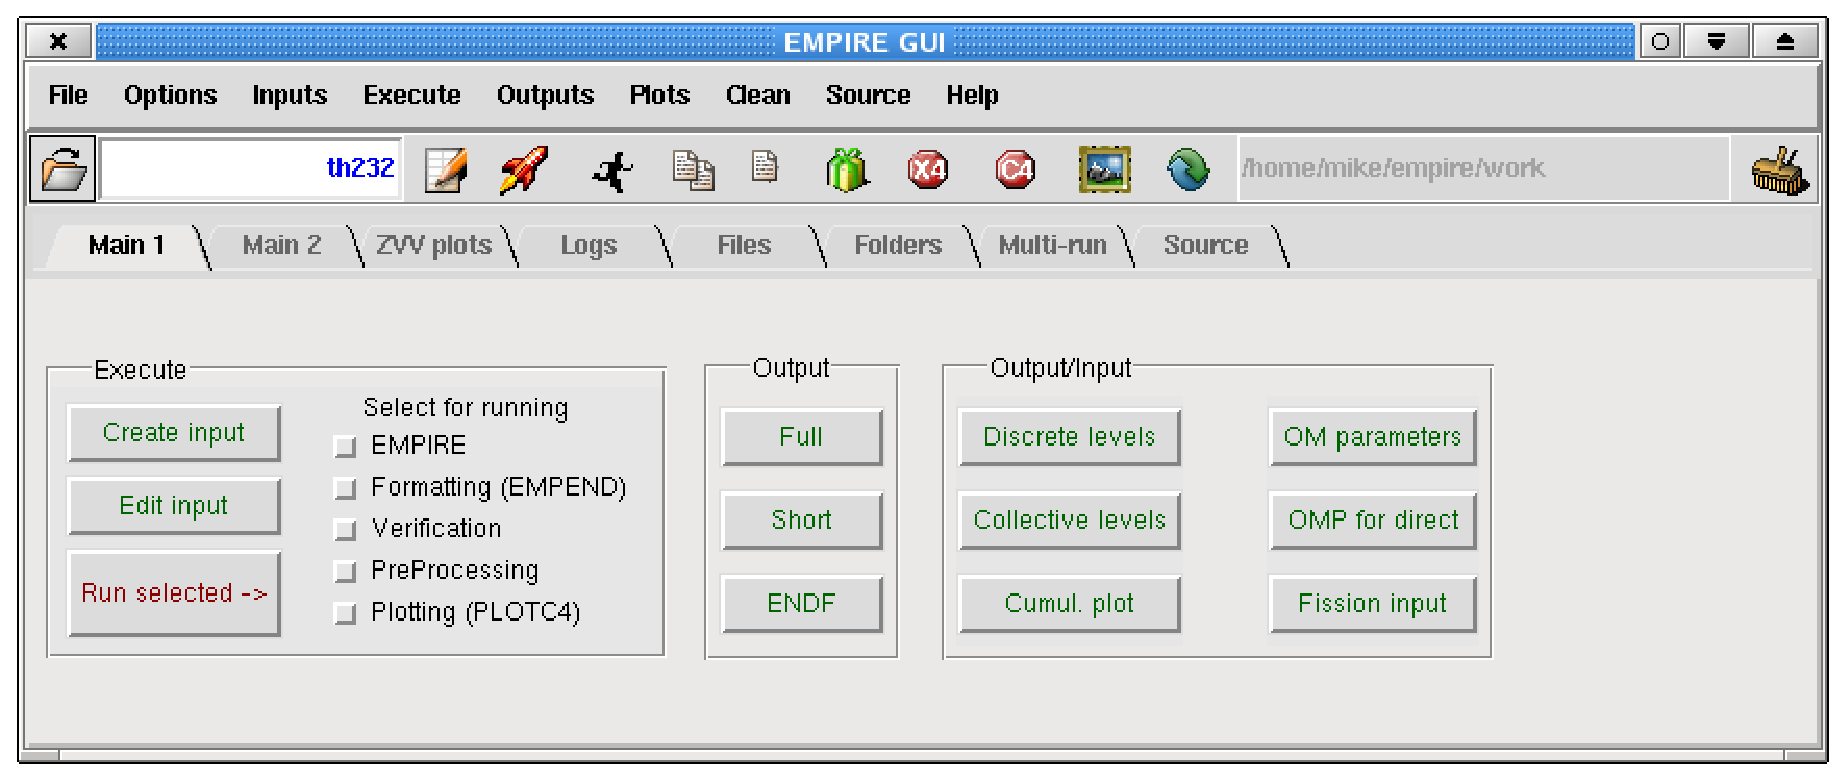
\includegraphics[width=0.75\paperwidth,bb = 0 0 200 100, draft, type=eps]{GUI-main1.eps}

\caption{\label{cap:EMPIRE-GUI-Main1}EMPIRE GUI - Main1 panel}

\end{figure}


We start discussion of the GUI with a few features that apply across
the entire interface:

\begin{itemize}
\item Action of many buttons is simply calling an appropriate script with
a project name as an argument. 
\item Double-click on the file in the list will generally open it with the
default application (i.e., text files will be open with the selected
editor, PostScript files with the selected viewer, and {*}.zvd files
will be displayed using ZVView). Within lists typical mouse selection
modes are usually available (although the first file only will be
open for editting): 

\begin{itemize}
\item a single-click selects the file,
\item continuous selection by dragging mouse with the left button pressed, 
\item continuous selection by clicking left mouse button while holding shift
key pressed at the end of the region, 
\item arbitrary multiple selection by clicking left mouse button while holding
'Ctrl' key pressed. 
\end{itemize}
\item Whenever Tcl/Tk allows a 'baloon-help' is showed when cursor remains
above the button or icon for a short period of time. This help is
hoped to be sufficient to operate the interface without additional
instructions. Note that if cursor is moved fast across the interface
the 'baloon-help' which appears on the screen might refer to a button
different from the one to which the cursor actually points. To be
sure that the help is correct keep in mind that help string always
starts exactly below the middle of a button or icon. 
\item Colours on the GUI buttons follow 'trafic light scheme' - green means
that pressing button at any time will not make any damage, red warns
that some data or files that have been obtained before or manually
editied might be lost (overwritten). Generally, all buttons involving
editor calls are green while button involving execution of codes or
deleting files are red. Similar distinction is introduced between
the files - red is used for those which are likely to have been manually
edited and green or orange for those which are easy to recreate by
rerunning the code .
\end{itemize}
Due to a large number of operations and extended lists the new GUI
is organized in a form of a notebook with several panels. Generally,
there are several equivalent ways of performing the same operation
and the user my choose the one which suits him best. All basic functions,
such as running the code and viweing the results can be achieved from
the pull-down menues and icon-denoted buttons below the menue bar.
On the other hand, more advanced features such a plotting and file
management can only be accessed from the various panels.

All operations (except multiple run) begin with selection of the project
name that will be used as a root of the input file name (say 56Fe).
Existing project can be selected by clicking on the 'open folder'
icon to the left of the GUI. The following icons (from left to right)
allow to (i) edit input, (ii) launch full chain of calculations, (iii)
run EMPIRE only, (iv) vew long EMPIRE output, (v) view short EMPIRE
output, (vi) view ENDF-6 formatted file, (vii) view EXFOR data, (viii)
view EXFOR data in computational format, (ix) view PLTC4 plots, (x)
refresh list of files, (xi) change working directory, and (xii) remove
all files related to the project except input. More operations are
possible from individual GUI panels.

\textbf{Main1 panel} - (Fig. \ref{cap:EMPIRE-GUI-Main1}) provides
for essential control of calculations. It allows to create a new input
file (clicking on the {}``Create'' button copies the standard input
file \emph{skel.inp} to \emph{56Fe.inp} and opens it for editing),
executing selected parts of the system (physics calculations, formatting,
verification, preprocessing and plotting). One should keep in mind,
that format verification and preprocessing can only be performed if
EMPIRE calculations and ENDF-6 formatting were carried out before,
and plotting is only possible starting from the preprocessed file.
Main1 panel gives also access to output and output/input files produced
by EMPIRE in the first run. 

\textbf{Main2 panel} - (Fig. \ref{cap:EMPIRE-GUI-Main2}) provides
additional four features for which there was not enough room on the
Main1 panel. %
\begin{figure}[top]
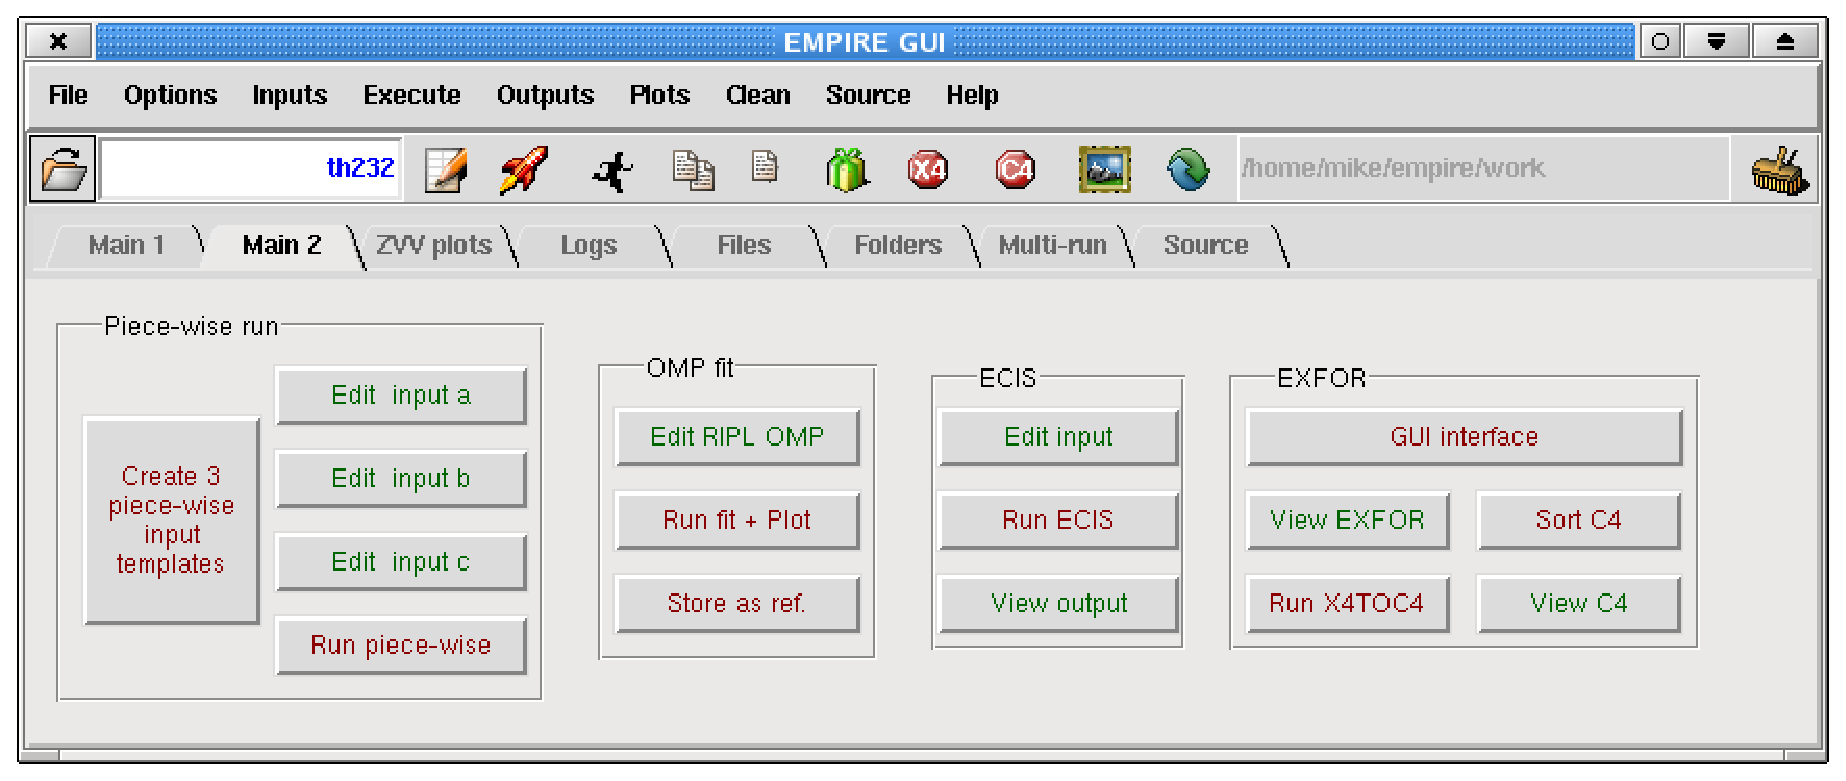
\includegraphics[width=0.75\paperwidth,bb = 0 0 200 100, draft, type=eps]{GUI-main2.eps}

\caption{\label{cap:EMPIRE-GUI-Main2}EMPIRE GUI - Main2 panel}

\end{figure}


\begin{itemize}
\item Piece-wise~run allows to run calculations using different input in
three non-overlapping energy ranges. Clicking on the 'Create 3...'
button makes 3 copies of the main EMPIRE input. These 3 copies can
be modified allowing for use of different parameters or models providing
that they refer to the same combination of target and projectile and
allow for the same number of emissions. The energy ranges must be
choosen is such a way that input \emph{a} covers the lower part, input
\emph{b} intermediate and input \emph{c} the upper part of the requested
energy range. When 'run-piecewise' button is hit caluclations are
executed for all three input files, respective outputs are merged
and the resulting file is formatted and processed as obtained in a
single run. Note that use of different parameters and models in the
three energy ranges will generally produce discontinuities at the
borders. The piece-wise calculations are also possible with 2 input
files only (the third one should be deleted in such a case). 
\item OMP fit section allows to run manual fit of the optical model potential.
EMPIRE provides limitted support by producing plots of selected cross
sections (angular distributions) and comparing them with the best
previous set. Input option FITOMP should be set to 1 to restrict calculations
to those relevant to optical parameter fitting (e.g., second neutron
emission will not be followed even though specified in the input).
After the first calculation is completed user should create up to
2 plots using right part of panel 'ZVV plots' (each of them may contain
a number of curves) and name them in the 'List name' field as \emph{omp1}
and \emph{omp2}. Then, optical model parameters can be adjusted manually
by editing respective files and calculations re-run. This will automatically
produce previously defined plots overlayed with those obtained in
the first run. If the new calculation performs better it can be set
as a temporary reference set by hitting the 'Store as ref.' button.
Next results will be compared to this reference until a new reference
is defined.
\item EXFOR section provides access to the stand alone EXFOR retrieval that
is graphically similar and functionaly identical to the one availabale
from the IAEA and NNDC web sites. Under normal cicumstances this retrieval
is not necessary as it is performed internally be EMPIRE during the
first run. However, user may choose to use manual retrieval interface
in order to exercise direct control on the retrieved data. When the
EXFOR interface is closed the resulting file with experimental data
is automatically renamed to conform to the current project. It is
up to the user to ensure that the data retrieved are actually relevant
to the calculations. Once retrieved, the data have to be converted
into the compuational format ('Run X4TOC4' button) and sorted ('Sort
C4' button). The same sequence of buttons should also be used if users
decides to modify the existing \emph{{*}.exf} file (e.g., by removing
or adding certain entries)
\item ECIS section allows to view the most recent input and output of ECIS03
code (note that these files are overwritten in each calculation for
each incident energy)
\end{itemize}
~

\textbf{}%
\begin{figure}[top]
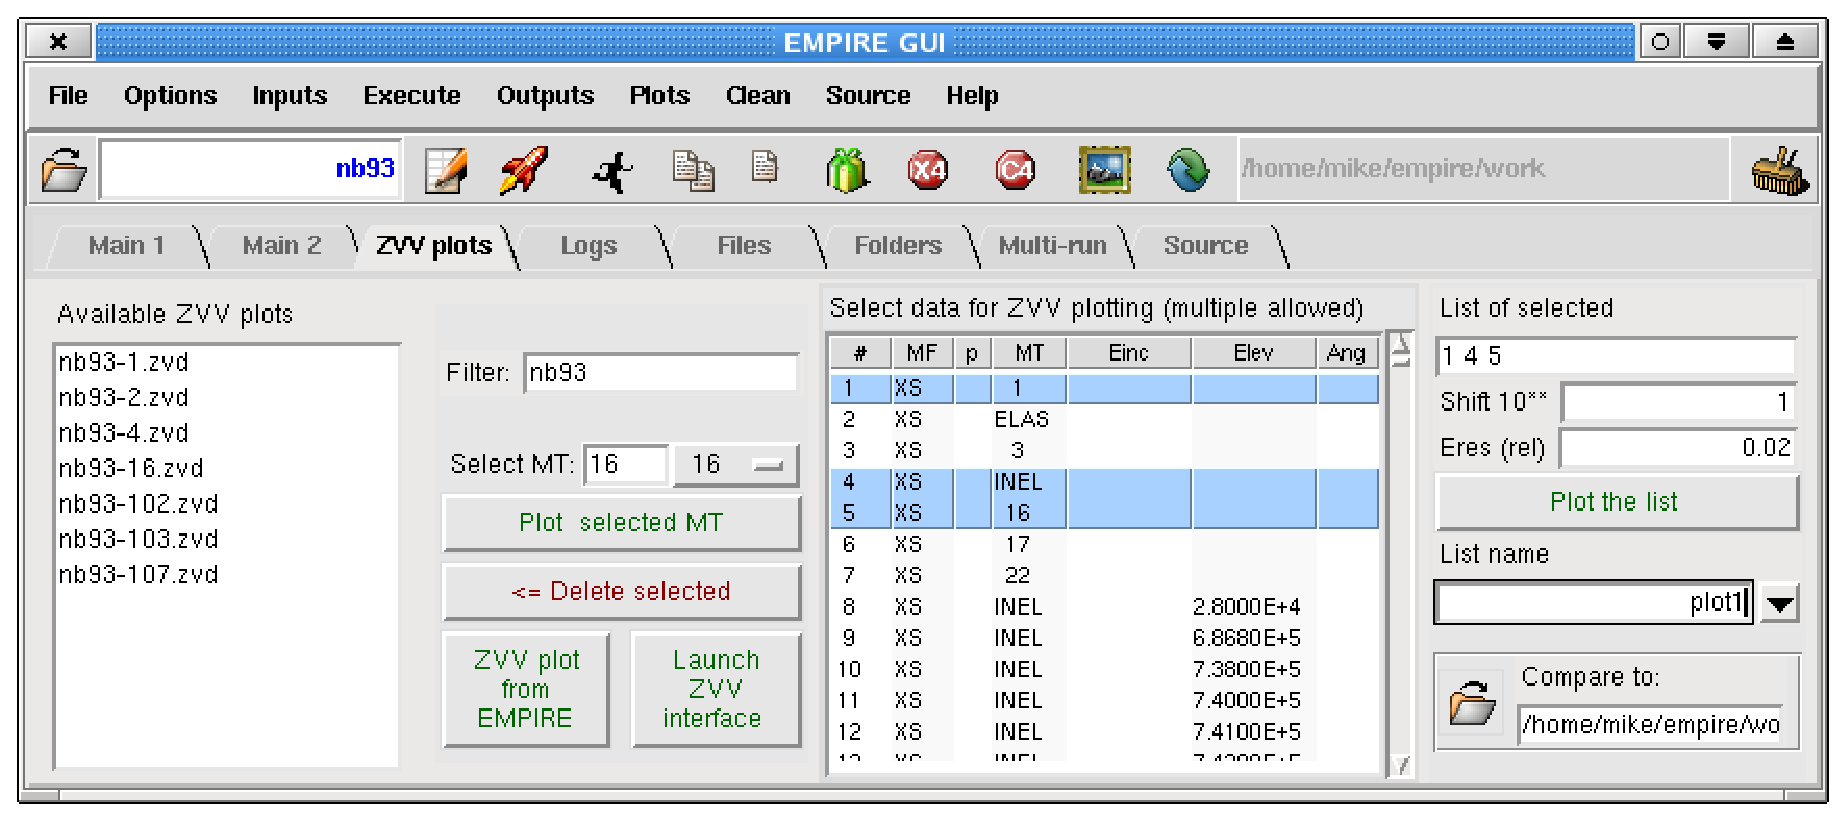
\includegraphics[width=0.75\paperwidth,bb = 0 0 200 100, draft, type=eps]{GUI-ZVV.eps}

\caption{\label{cap:EMPIRE-GUI-ZVV}EMPIRE GUI - ZVView plots panel}

\end{figure}
\textbf{ZVV plots panel} (Fig. \ref{cap:EMPIRE-GUI-ZVV}) provides
for a powerfull interface to the ZVView plotting package. The window
to the left lists all ZVView plots (\emph{{*}.zvd} files) that have
been previously created. User can display them by doubleclicking on
any of them. Selecting several plots and doubleclicking on the last
one will combine all the selected curves into a single plot. Note
that 'Filter' field allows to restrict displayed files to those containing
filter string in the name (by default Filter is set to the project
name). There are 4 possibilities of creating ZVView files:

\begin{itemize}
\item Selecting MT number and hitting 'Plot selected MT' (note that any
valid ENDF-6 MT number can be typed into the field in addition to
those which can be selected from the predefined list). The MT number
is included in the plot filename for identification (e.g., \emph{56Fe-102.zvd}
for capture). This method allows to plot only excitation functions
(cross sections) for the current calculations (ENDF-6 formatted file
must exist).
\item Hitting 'Launch ZVV Interface' will start more powerfull GUI that
allows to create the same type of plots as before but including up
to 3 additional ENDF-6 formatted files for comparison. 
\item 'ZVV plots from EMPIRE' is bit cumbersome way of creating a cross
section ZVView plot by selecting unique string identifying output
line containing the cross section of interest, pasting it into the
other window and filling additional information (next line, title,
etc.) as requested. The advantage of this method is that the ENDF-6
formatted file is not required and any cross section (number followed
my 'mb') in the long output (\emph{{*}.lst}) can be plotted. This
includes quantities that can not be plotted with the previous methods
since not stored in the ENDF-6 formatted file (such as cross sections
for the population of discrete levels in any nucleus or intensities
of $\gamma$-rays).
\item Selecting plots from the window to the right of the GUI (list created
by PLOTC4 or \emph{pltlst} script). This is the only possibility of
plotting angular distributions, and energy spectra with the ZVView
package. For the relevant line being included in the list there must
be a match between experimental data and calculations (i.e., plots
are only possible if adeqaute experimental data are available). Multiple
selection can be plotted and each of such selections can be stored
by specifying its name in the 'List name' field. When multiple selection
is plotted the individual curves are offset from each other by a number
of decades specified in the 'Shift 10{*}{*}' field. It implies that
the \emph{y}-scale be logarithmic unless shift is set to 0. 'Eres
(rel)' is the experimental relative energy resolution used to spread
discrete lines (e.g., elastic) and to smooth continuum in the plotted
energy spectra. The 'Comapre to' field allows to select another ENDF-6
formatted file to be included in the plots. Note that in order to
obtain correct plots the additional file should be preprocessed in
a way analogous to the original EMPIRE file (otherwise resonances
might not be plotted since not reconstructed and File 6 data might
not be in a right format).
\end{itemize}
~

\textbf{}%
\begin{figure}[top]
\includegraphics[width=0.75\paperwidth,bb = 0 0 200 100, draft, type=eps]{GUI-Logs.eps}

\caption{\label{cap:EMPIRE-GUI-Logs}EMPIRE GUI - Logs panel}

\end{figure}
\textbf{Logs panel} (Fig. \ref{cap:EMPIRE-GUI-Logs}) provides access
to various output files that should be inspected for possible errors
encountered during EMPIRE execution, EXFOR translation into compuational
format, ENDF-6 formatting, format verification and preprocessing.%
\begin{figure}[top]
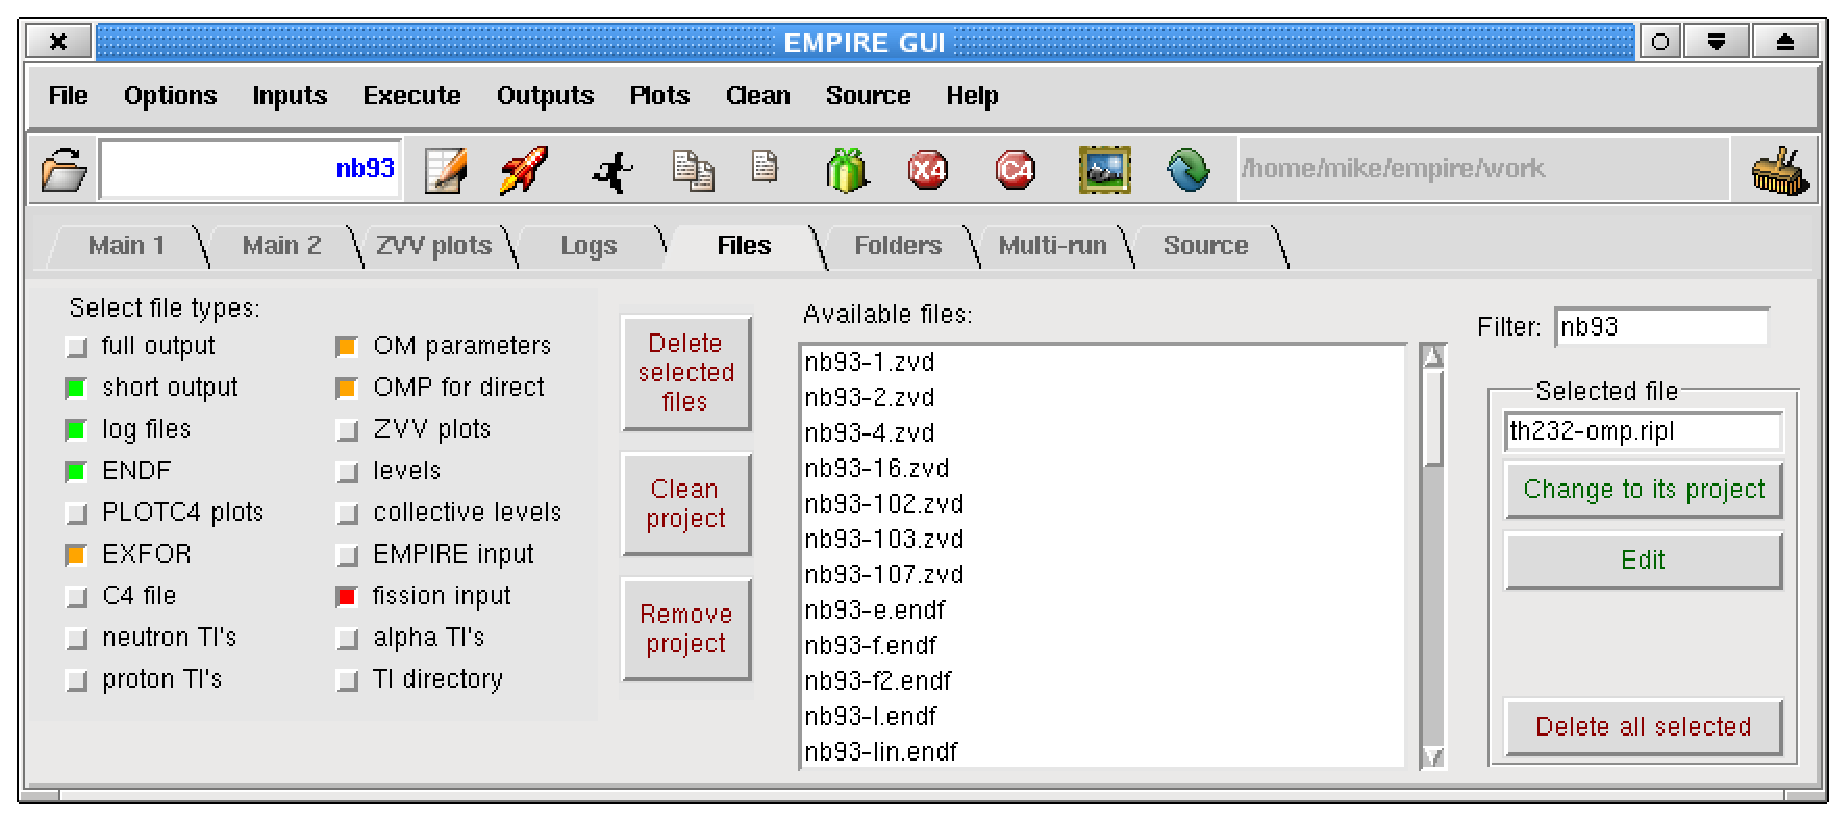
\includegraphics[bb = 0 0 200 100, draft, type=eps]{GUI-Files.eps}

\caption{\label{cap:EMPIRE-GUI-Files}EMPIRE GUI - Files panel}

\end{figure}


\textbf{Files panel} (Fig. \ref{cap:EMPIRE-GUI-Files}) offers file
management functions tailored to facilitate operation of the EMPIRE
code. Large number of files produced in a single EMPIRE run might
result in a very crowded working directory if the latter contains
several projects. Files panel is designed to facilitate access to
files belonging to a current project by setting default value of the
filter to the root-name of the project. User can modify filter value
to restrict further list of the files (e.g., filter set to \emph{56Fe{*}endf}
will show only files with extension {*}.\emph{endf} beloging to the
\emph{56Fe} project) or relax it to display more files (e.g., filter
set to \emph{inp} will show input files for all projects). We note
that, selecting a file with a name consisting only of the root-name
and extension (e.g., \emph{56Fe.exf} but not \emph{56Fe-log.psyche)}
and hitting 'Change to its project' button is a convienient way of
redirecting GUI toward another project. The left part of the panel
provides for a convenient removal of the selected types of files belonging
to the current project. In addition, individual files can be removed
by clicking on the 'Delete all selected' button. A double-click on
any of the listed files will open it with an appropriate application.

\textbf{Folders panel} - (Fig. )

\textbf{Multirun panel} - (Fig. )

\textbf{Source panel} - (Fig. )

\emph{To be completed}

%
\begin{figure}[top]
\includegraphics[bb=0bp 0bp 219bp 973bp,height=0.3\paperwidth,bb = 0 0 200 100, draft, type=eps]{GUI.eps}

\caption{\label{fig: GUI}Old EMPIRE GUI}

\end{figure}


\textbf{Obsolate EMPIRE GUI (lrun.tcl)}

The previous version of the EMPIRE graphic interface \textbf{(lrun.tcl)}
is no more maintained but is still provided since it does not require
\emph{itcl} package and therefore can be run on systems lacking this
feature. It allows for basic operation of the code but its capabilities
are very limited compared to \textbf{Xrun.tcl}. The old GUI is shown
in Fig. \ref{fig: GUI}, and is invoked by typing \\


\begin{quotation}
\texttt{\small ../scripts/lrun.tcl \&}{\small \par}
\end{quotation}
in the \emph{empire/work} subdirectory. Users have to specify a project
name that will be used as a root of the input file name (say 56Fe).
A new input file can be created by clicking on the {}``Create''
button to copy the standard input file \emph{skel.inp} to \emph{56Fe.inp}
and open for editing. Buttons in the {}``Execution'' section correspond
to the scripts described in the preceding section. Output files can
be edited by clicking the appropriate button in the section {}``Outputs''.
The {}``Clean'' button invokes the \emph{clean} script, and removes
most of the case related files. GUI also offers the possibility of
changing EMPIRE source files and modifying the dimensions. One has
to click on the {}``Make'' button to issue the \emph{'make'} command
in the \emph{empire/source} subdirectory and recompile the code. The
{}``Options'' menu allows modifications to the EMPEND\index{EMPEND},
FIXUP\index{FIXUP} and PLOTC4\index{PLOTC4} input files and the
default EMPIRE input file \emph{skel.inp} . The same menu also permits
the selection of the preferred editor used within GUI. At present,
the following X-windows editors are included: \emph{gvim (vi), emacs,
nedit, kedit, jove,} and \emph{GXedit}. It should be stressed that
EMPIRE GUI uses editors installed on the system. Although, some of
those mentioned above may not be directly available, the possibility
exists to incorporate additional editors not included in the list.
To this end one has to edit \emph{empire/work/lrun.tcl} file, locate
the lines

\begin{quotation}
\texttt{\$base.cpd32.men40.01.02 add radiobutton \textbackslash{}}

\texttt{~~~-command \{set editor \{gvim\}\} -label gvim -value
gvim}
\end{quotation}
replicate both of them and change {}``gvim'' to any desired editor.
For example, if the new editor is called {}``fred'', the resulting
piece of Tcl script should be 

\begin{quotation}
\texttt{\$base.cpd32.men40.01.02 add radiobutton \textbackslash{}}

\texttt{~~~ -command \{set editor \{gvim\}\} -label gvim -value
gvim}

\texttt{\$base.cpd32.men40.01.02 add radiobutton \textbackslash{}}

\texttt{~~~ -command \{set editor \{fred\}\} -label fred -value
fred}
\end{quotation}
The short description of the EMPIRE input, list of RIPL\index{RIPL}-2
OM potentials, and manuals of the utility codes can be brought to
the screen from the 'Help' menu.


\section{ENDF formatting}

The ENDF formatted file is created by the user selecting the ENDF
option in the input file ({*}.\emph{inp}). This instructs EMPIRE to
write all necessary information to the output file \emph{{*}.out},
which may actually become long! This file is processed by the utility
code EMPEND\index{EMPEND}, which creates the ENDF-6 formatted file.
Two distinct options are available 

\begin{labeling}{MMMMMM}
\item [{ENDF~~~~1.}] exclusive spectra (classical ENDF-6 representation)
\item [{ENDF~~~~2.}] inclusive spectra.
\end{labeling}
While the physical calculations performed by EMPIRE with the ENDF=2
option are the same, the results are transferred for formatting in
a different form. Rather than providing exclusive cross sections and
associated spectra for each of the reactions separately, EMPIRE outputs
inclusive cross sections, spectra and double-differential cross sections.
In other words, total emission spectra of neutrons, protons, $\alpha$-particles
and $\gamma$s are printed instead of individual contributions from
various reactions. EMPEND\index{EMPEND} automatically recognizes
the ENDF options and acts accordingly using MT=5 and specifying relative
yields of the products in MF=6 if ENDF is set to 2. 

The EMPIRE output ({*}.\emph{out}) is processed and converted into
ENDF format by the EMPEND code written by Trkov. The ENDF formatted
output file has to obey the rule of defining the reactions in increasing
order by MT reaction number, so several sweeps of the EMPIRE file
({*}.\emph{out}) are made: 

\begin{itemize}
\item first sweep: the cross sections and the corresponding reaction Q-values
are extracted,
\item second sweep: all reactions are identified for which particle spectra
are given, 
\item third sweep: to identify each reaction requiring an ENDF file-4 section;
these data are entered for discrete level reactions,
\item fourth sweep: to identify each reaction that has outgoing energy-angle
correlated particle distributions, 
\item finally, a sweep is made for the remaining reactions, particularly
the (n,$\gamma$) reaction, for which the distributions are coded
in ENDF Files-12, 14 and 15. 
\end{itemize}
The cross section data found on the file are fitted by a cubic spline
and entered into the output ENDF file (\emph{{*}.endf}) on a user-defined
dense energy grid, thinned to the specified tolerance and taking reaction
thresholds into account. If desired, the spline interpolation may
be suppressed and the energy points found on the file are entered
directly into the ENDF formatted file.

The angular distributions for discrete level reactions that appear
in the ENDF file-4 sections are extracted from the spectra on the
EMPIRE output file ({*}.\emph{out}), and interpolated to the appropriate
energy, if necessary.

The correlated energy-angle distributions for continuum reactions
that appear in ENDF file-6 sections are entered as Legendre polynomial
representations in the center-of-mass coordinate system. The maximum
Legendre order is limited to 12. For reactions with relatively smooth
angular distributions, the number of coefficients is reduced accordingly.
Photon production reactions, which remain to be specified, particularly
the (n,$\gamma$) reaction, are given in the ENDF files-12, 14 and
15. Photon multiplicity is stored in file-12. Isotropic angular distribution
is assumed and written to file 14. The particle energy distribution
is written to file 15. 

The program can be executed interactively from a terminal screen.
The non-interactive version is called by the script \emph{format}
and from the GUI. When the interactive version is executed the required
input is entered in response to the prompts, which are as follows: 

\begin{itemize}
\item Name of the EMPIRE output file to be processed. 
\item Name of the ENDF formatted file to be written. 
\item Number of sub-intervals per incident neutron energy interval on the
EMPIRE output file. The sub-intervals define the fine energy mesh
on the ENDF formatted file. If zero is entered, only the points on
the EMPIRE output are entered to the ENDF formatted file. 
\item Thinning tolerance limit {[}\%] to reduce the number of cross section
points. Data points are removed that can be reproduced from the neighboring
points by linear interpolation to within the specified tolerance.
Entering a negative value for the thinning tolerance limit causes
thinning to be suppressed. 
\item ENDF material number identifier. 
\end{itemize}
In the non-interactive mode these data are read from the input file
\emph{empire/work/EMPEND.INP}, which is available for editing from
the GUI. 

The formatting process is recorded for quality assurance purposes
by writing the details in the \emph{EMPEND.LOG} file. A limited amount
of checking is done. An entry is added to the log file in the following
cases: 

\begin{itemize}
\item The cross section obtained by integrating the spectrum should agree
with the value given directly in the EMPIRE output file (\emph{.out}).
If the difference exceeds 2\%, a warning message is written that lists
the MT reaction number, the incident particle energy, the expected
cross section (i.e. value given directly in the EMPIRE output file)
and the percent difference. 
\item The angular distributions are fitted to determine the Legendre polynomial
expansion coefficients. If the distribution reconstructed from the
Legendre polynomial coefficients differs from the point-wise values
on the EMPIRE output file by more than 5\%, a warning message is written
that gives the reaction MT number, the outgoing particle ZA identifier,
the incident and the outgoing particle energies and the percent difference
in the fitted distribution from the point-wise value on the file. 
\end{itemize}
Additional messages monitor the progress of the data formatting process.


\section{Fitting Optical Model Parameters}

When the FITOMP option is selected in the input, EMPIRE will perform
automatic fitting of parameters in the direct optical model parameter
file, OMPAR.DIR ({*}-omp.dir), and of deformation parameters in the
file containing the collective target levels, TARGET\_COLL.DAT ({*}-lev.col).
The fitting procedure also uses the experimental data file in C4 format,
C4.dat ({*}.c4). To ensure the existence of these files, EMPIRE should
be executed at least once before fitting begins and should be executed
with the DIRECT option selected and an incident channel optical potential
(initially) defined using the DIRPOT option, both in the initial run
and during fitting. At the moment, the FITOMP option only works for
neutron or proton scattering. 

All data relevant to an optical model fit - total, elastic and collective
inelastic cross sections and elastic and collective inelastic angular
distributions - within the requested energy range are selected from
the C4.dat file and included in the $\chi^{2}$ to be minimized. The
data points in the $\chi^{2}$are weighted in the standard manner
using the experimental uncertainties given in the C4.dat file. Natural
element data can be inserted in the C4.dat file and used in the fit.
In the case of neutron scattering, the file \emph{empire/RIPL-2/resonances/resonances0.dat}
is also searched for an s-wave strength function, which is included
in the experimental data set when found. 

The lower limit of the energy range for calculations used in a fit
is initially taken to be 1 keV while the upper limit is taken to be
30 MeV, unless modified using the FITEMX option in the input. All
relevant experimental data within this range in the C4.dat are included
in the $\chi^{2}$. The incident energies given in the input file
define the grid of energies used for calculations, unless the FITGRD
option is used. When the input file energies are used, the data points
outside of the energy interval they define are not taken into account.
That is, the fitting procedure will interpolate calculations but will
not extrapolate them. When the FITGRD option is used, the energy interval
is extended to include all data points in the initial energy range.
In both cases, the grid of incident energies is compared with those
of the experimental data and superfluous values are eliminated to
speed up the calculation. 

The parameters to be adjusted are specified by using the FITabc or
FITDEF options, described in more detail below. The RIPL-2 parametrization
described in Section \ref{sec:RIPLomp} is used to identify the optical
model parameters, any of which may be adjusted. The adjustable deformations
are simply those of the collective level file. Quadrupole and hexadecupole
deformations are permitted for nuclei identified as rotational, while
quadrupole and octupole deformations are permitted for those identified
as vibrational. The FITabc and FITDEF options typically identify the
desired parameter and furnish a shift in its initial value and the
maximum variation allowed during the fit with respect to its (shifted)
initial value. If no parameter adjustment is requested or all adjustable
(possibly shifted) parameters have a maximum allowed variation of
zero, the $\chi^{2}$ is calculated but no fitting is performed. At
most 20 parameters may be shifted and/or adjusted simultaneously.

At present, the optical model fitting is performed using a simple
numerical gradient search to minimize the $\chi^{2}$. The adjusted
parameters are stored in the modified OMPAR.DIR ({*}-omp.dir) and
TARGET\_COLL.DAT ({*}-lev.col) files. Information on the fit is written
in the FIT.OUT ({*}-ompfit.lst) file. When a fit is complete, EMPIRE
is run one last time with all options and energies given in the input
file, excepting the fit ones. 


\section{Input/Output files}


\subsection{\label{sec: input}{*}.inp (INPUT.DAT; main input)}

EMPIRE is set up to read as much data as possible from the input parameter
library (\emph{empire/data}). The user has to supply only those input
parameters that the code can not know. These are the incident energy,
the projectile, the target and the number of neutron, proton, $\alpha$,
and light-ion emissions to be followed. In principle, the number of
emissions could be eliminated by following the compound nucleus de-excitation
until all the energy is exhausted. However, this is not very practical,
as in most cases a very large amount of memory would have to be allocated
and a lot of CPU time consumed to calculate exit channels that might
be of no interest. 

With the default library of input parameters it is possible to execute
a 'first-shot' calculation with minimal effort. In the second step,
the user may wish to regain control over the input in order to make
appropriate adjustments to the parameters. This can be done in a selective
way in the optional part of the EMPIRE input. 

It should be noted that there is a difference in the way EMPIRE accesses
general input library in the first and subsequent runs of a given
project. In the first run the code extracts relevant data from the
input parameter library and creates files with discrete levels ({*}.\emph{lev}),
collective levels (\emph{{*}-lev.col}), optical model parameters \emph{({*}-omp.ripl,}
and \emph{{*}-omp.dir)} and relevant EXFOR data ({*}.\emph{exf} and
{*}.\emph{c4}). Once these files exist the code uses them instead
of the files contained in the general input library. This has two
advantages: (i) time is spared because the case specific files are
small and can be read fast, (ii) the user may edit {*}.\emph{lev,
{*}-omp}.{*}, and {*}.\emph{c4} files and modify them without affecting
files in the general input library. Editing the \emph{{*}-omp.{*}}
files is a convenient method of adjusting some of the optical model
parameters without the necessity of typing the whole set from scratch.

Input data are taken from different sources in the following order
(those listed above overwrite those listed below):

\begin{enumerate}
\item case specific files (\emph{{*}.lev, {*}-lev.col, {*} .fus, {*} -omp}.{*})
\item input file ({*}.\emph{inp})
\item general input parameter library
\end{enumerate}
Note, that all the files, except \emph{{*}.inp}, are created by the
code during the first run, and therefore the user has to create only
the {*}.\emph{inp} file described below.


\subsubsection*{Mandatory input}

Input to EMPIRE consists of two parts. The first is mandatory and
contains basic data necessary to specify the case, and the structure
is illustrated by the following example: 

\begin{labeling}{MMMMMMMMM}
\item [{\texttt{\footnotesize 14.8}}] \texttt{\footnotesize ;INCIDENT ENERGY
(IN LAB) }{\footnotesize \par}
\item [{\texttt{\footnotesize 56.~~26.}}] \texttt{\footnotesize ;TARGET
 A , Z }{\footnotesize \par}
\item [{\texttt{\footnotesize 1.~~0.}}] \texttt{\footnotesize ;PROJECTILE
A, Z}{\footnotesize \par}
\item [{\texttt{\footnotesize 3}}] \texttt{\footnotesize ;NUMBER OF NEUTRONS
TO BE EMITTED}{\footnotesize \par}
\item [{\texttt{\footnotesize 1}}] \texttt{\footnotesize ;NUMBER OF PROTONS
 TO BE EMITTED}{\footnotesize \par}
\item [{\texttt{\footnotesize 1}}] \texttt{\footnotesize ;NUMBER OF ALPHAS
  TO BE EMITTED}{\footnotesize \par}
\item [{\texttt{\footnotesize 0~~0.~~0.}}] \texttt{\footnotesize ;NUMBER
OF L.I.  TO BE EMITTED AND ITS A AND Z}{\footnotesize \par}
\end{labeling}
The first line specifies the incident energy in the laboratory system
(in MeV). The second and third are used to specify the masses and
atomic numbers of a target and a projectile respectively. The next
three lines define the number of emissions to be followed for each
ejectile. In the above example, all reactions up to (n,3np$\alpha$)
will be calculated. The code automatically sums over all possible
decay sequences to reach the given residual nucleus. Accordingly,
$\sigma_{(n,3np\alpha)}=\sigma_{(n,2npn\alpha)}+\sigma_{(n,np2n\alpha)}+\sigma_{(n,p3n\alpha)}+\sigma_{(n,\alpha3np)}+...$
includes all possible permutations of ejectiles. The last line of
the input provides for the inclusion of the emission of one type of
light ion. The library of optical model parameters allows for d, t,
$^{3}$He, $^{6}$Li, $^{7}$Li, and $^{7}$Be ejectiles. Use of the
light ion ejectile option requires the code to be compiled with NDEJC
set to 4 in the file \emph{dimension.h}. If the last line of the mandatory
input consists of three zeros (as in the example) the light ion emission
channel is closed regardless of the NDEJC value used in the compilation.
The mandatory part of the input is in a free format, while the comments
following the semicolon only serve to facilitate input preparation
and are ignored by the code.


\subsubsection*{Optional input}

The mandatory input is followed by optional input, which allows modifications
to the default model parameters. Optional input consists of an arbitrary
number of records, entered in any order and closed with the GO record,
which indicates the end of the input. In the simplest case (all defaults),
only the GO record must be entered. Each record starts with an alphanumeric
keyword NAME which is followed by the value VAL and the positional
parameters. The keyword indicates a physical quantity, such as the
binding energy or level density parameter or an option. VAL takes
the numerical value of the quantity or option. The positional parameters
are typically used to specify to which nucleus the quantity should
be applied. Each record must be in the format:

\begin{quote}
FORMAT (A6,G10.5,4I5) NAME,VAL,I1,I2,I3,I4
\end{quote}
The GO record may be followed by an unlimited list of incident energies
(one per record) terminated with a record containing a negative value.
Anything below this line will be ignored by the code. The distribution
of EMPIRE contains a number of sample inputs.

A complete list of model parameters and options that can be controlled
through the optional input entries is given below.


\subsubsection*{Calculation control}

\begin{labeling}{00.00.0000}
\item [{NEX}] Maximum number of energy steps in the integration set to
VAL (default: min(50, NDEX)).
\item [{LTURBO}] Step in the angular momentum set to VAL. This option can
be used to speed up Heavy Ion calculations. For example, setting LTURBO
to 2, only each second spin in the Compound Nucleus and in all residual
nuclei will be considered. The result is appropriately normalized
so that no flux is lost (default: 1).
\item [{ENDF}] Controls output for ENDF formatting,\\
= 1 output for the ENDF formatting will be created,\\
= 0 no output for the ENDF formatting will be created (default).
\item [{FITPOT}] Controls optical model fitting (only total, elastic, capture
and inelastic cross sections and elastic and inelastic angular distributions
can be fit),\\
= 1 automatic optical model fitting will be performed,\\
= 0 no optical model fitting will be performed (default).
\item [{KALMAN}] Controls calculation of a sensitivity matrix,\\
= 1 sensitivity matrix will be calculated,\\
= 0 no sensitivity matrix will be calculated (default).
\end{labeling}

\subsubsection*{Output control}

\begin{labeling}{00.00.0000}
\item [{IOUT}] Main output control set to VAL ,\\
= 0 no output except warnings, \\
= 1 input data and essential results (all cross sections) (default),
\\
= 2 as IOUT=1 plus fusion spin distribution, yrast state population,
$\gamma$-transition parameters, fusion barrier, inclusive spectra,
\\
= 3 as IOUT=2 + $\gamma$ and particle spectra + discrete levels'
decay + double differential cross sections (if MSD\index{MSD}$>$0),
\\
= 4 as IOUT=2 + ORION\index{ORION} output + residual nuclei continuum
population (up to spin 12), \\
= 5 as IOUT=2 + ORION output + transmission coefficients (up to l=12),
\\
= 6 as IOUT=2 + ORION output + level densities\index{level densities}
(up to spin 12).
\item [{NOUT}] MSC\index{MSC} calculation output control set to VAL (default:
0).
\end{labeling}

\subsubsection*{Fusion\label{sec: InpFus}}

\begin{labeling}{00.00.0000}
\item [{FUSRED}] Fusion cross section will be multiplied by VAL (default:
1.).
\item [{CSREAD}] Controls HI fusion cross section determination,\\
$>$ 0 HI fusion cross section is set to VAL {[}in mb], \\
= -1 distributed barrier model used ,\\
= -2 Coupled-Channels\index{Coupled-Channels} CCFUS\index{CCFUS}-code
used (default for HI).\\
 Note: CSREAD has no effect if .\emph{fus} file (\emph{FUSION} in
manual mode) exists.
\item [{BFUS}] Fusion barrier height in the distributed barrier model (Eq.
\ref{distbarr}) set to VAL (default: $B_{fus}$ calculated by CCFUS\index{CCFUS}).
\item [{SIG}] SIGMA in the distributed barrier model (Eq. \ref{distbarr})
set to VAL (default: $0.05B_{fus}$).
\item [{TRUNC}] Truncation in the distributed barrier model (Eq. \ref{distbarr})
set to VAL (default: 2.).
\item [{EXPUSH}] Extra-push energy set to VAL (default: 0.).
\item [{CRL}] Critical \emph{l}-value for HI fusion (Eq. \ref{Tlfus})
set to VAL (default: 0).
\item [{DFUS}] Diffuseness in the transmission coefficients for HI fusion
(Eq. \ref{Tlfus}) set to VAL (default: 1.).
\item [{TRGLEV}] Excited level of the target is set to VAL (default: 1
(ground state)).
\end{labeling}

\subsubsection*{Width fluctuations (HRTW)}

\begin{labeling}{00.00.0000}
\item [{HRTW}] Controls HRTW calculations \\
= 0 no HRTW \\
= 1 HRTW up to 5 MeV incident energy, and no HRTW above this value
(default) \\
= 2 HRTW for all incident energies
\end{labeling}

\subsubsection*{CCFUS\index{CCFUS} input}

\begin{labeling}{00.00.0000}
\item [{DV}] DV barrier parameter in CCFUS set to VAL. This parameter can
be used to adjust the fusion barrier. Typical range for changes -10<DV<10.
(default: 10).
\item [{FCC}] FCC parameter in CCFUS\index{CCFUS} set to VAL,\\
=0 diagonalization of the coupling is performed at the barrier position
$r_{b}$,\\
=1 exponential character of the form factor is taken into account.
A second order estimation of the position and height of the effective
barriers is carried out within a one-Fermi distance from $r_{b}$.
This option is recommended for strong coupling (default). 
\item [{NSCC}] Number of inelastic surface channels in CCFUS\index{CCFUS}
set to VAL (default: 4).
\item [{NACC}] Number of additional channels set to VAL (default: 0).
\item [{BETCC}] Deformation of the I2$^{th}$ collective mode set to VAL.
\item [{FLAM}] Multi-polarity of the I2-th collective mode set to VAL (entered
with positive sign for target modes and negative sign for projectile
modes) (default:~ 2, 3, -2, -3, needs NSCC numbers).
\item [{QCC}] Q-value of the I2$^{th}$ collective channel set to VAL -
excitation energy of the collective level adopted with a negative
sign (default: - energies of the first 2+ and 3- levels in the target
and the projectile). 
\item [{FCD}] Strength of the coupling at the barrier for I2$^{th}$ collective
mode set to VAL. For FCC=1 the characteristic radial dependence of
the one-particle transfer form factor is assumed. Used only if NACC>0
(no default).
\end{labeling}

\subsubsection*{Coupled-Channels\index{Coupled-Channels} (ECIS)\index{ECIS}}

\begin{labeling}{00.00.0000}
\item [{DIRECT}] Controls use of ECIS03 \\
=0 spherical OM used (default) \\
=1 Coupled Channel method used for calculation of inelastic scattering
to collective levels. If a selected OM potential is of CC type, the
elastic and reaction cross sections are also taken from ECIS03. Otherwise,
spherical OM results are used. In any case, transmission coefficients
for all emissions are calculated with spherical OM \\
=2 as above but all transmission coefficients for the incident nucleon
emission are calculated within Coupled Channel approach with ECIS03\index{ECIS}
(extensive calculation time). \\
=3 as DIRECT=1 but DWBA\index{DWBA} is used instead of CC. All transmission
coefficients calculated with spherical OM \\
NOTE: OM potential to be used by ECIS03 might be different from the
one used in the rest of the calculations and can be specified with
the DIRPOT option.
\item [{EcDWBA}] Selects all levels with energy below VAL and spin equal
or less than I1 to be used in DWBA calculations performed parallel
to CC.
\end{labeling}

\subsubsection*{Multi-step Direct}

\begin{labeling}{00.00.0000}
\item [{MSD\index{MSD}}] Controls Multi-step Direct\index{MSD} calculations
,\\
= 0 no MSD calculations (default),\\
= 1 MSD calculations selected - ORION\index{ORION} + TRISTAN\index{TRISTAN}
will be executed,\\
= 2 MSD calculations selected but only TRISTAN will be executed using
the most recent results of ORION. WARNING! there is no check whether
the last and the current run match with regard to the projectile,
the target and the incident energy; this option can be used for a
single incident energy only.
\item [{WIDEX}] Experimental energy resolution set to VAL (default: 0.2).
\item [{GAPP}] Proton pairing gap for target set to VAL (default: $12/\sqrt{A}$
).
\item [{GAPN}] Neutron pairing gap for target set to VAL (default: $12/\sqrt{A}$
).
\item [{HOMEGA}] $\hbar\omega$ oscillator energy (default: 41.47/A$^{1/3}$
MeV ).
\item [{EFIT}] Coupling constants of multi-polarity I1 fitted to the level
at energy VAL (defaults: -1 for $\lambda=0$, $E_{GDR}$ for $\lambda=1$,
energies of the first low-lying 2+, 3-, and 4+ levels for $\lambda=2,\,3,\,4$,
respectively).
\item [{RESNOR}] Response function for multi-polarity I1 will be normalized
by factor VAL (default: 1).
\item [{ALS}] spin-orbit coupling strength in the harmonic oscillator (default:
1.5).
\end{labeling}

\subsubsection*{Multi-step Compound }

\begin{labeling}{00.00.0000}
\item [{MSC\index{MSC}}] Controls Multi-step Compound\index{MSC} calculations,\\
= 0 no MSC calculations (default),\\
= 1 MSC calculations selected.
\item [{XNI}] Initial exciton number set to VAL (default set internally
depending on the case, 3 for nucleon induced reactions).
\item [{GDIV}] Single particle level densities in MSC set to A/VAL (default:
13.0).
\item [{TORY}] Ratio of unlike to like nucleon-nucleon interaction cross
section set to VAL. Used for the determination of the relative share
between neutron and protons in the exciton configurations (default:
4.).
\item [{EX1}] Initial number of excitons that are neutrons set to VAL (default
set internally depending on the case and on TORY).
\item [{EX2}] Initial number of excitons that are protons set to VAL (default
set internally depending on the case and on TORY).
\item [{D1FRA}] Ratio of the spreading GDR width to the total GDR width
set to VAL (default: 0.8).
\item [{GST}] Controls $\gamma$-emission in MSC\index{MSC},\\
= 0 no $\gamma$-emission in MSC (default),\\
= 1 $\gamma$-emission in MSC selected.
\item [{STMRO}] Controls \emph{p-h} level density\index{p-h level density}
calculations, \\
= 0 closed form \emph{p-h} state densities selected (default),\\
= 1 microscopic \emph{p-h} state densities selected (not yet implemented).
\end{labeling}

\subsubsection*{Exciton model (DEGAS\index{DEGAS})}

\begin{labeling}{00.00.0000}
\item [{DEGAS}] Controls exciton model calculations, \\
= 0 DEGAS code disabled (default),\\
= 1 DEGAS code enabled.
\item [{GDIVP}] Sets single-particle level density parameter (g) for protons
to A/VAL (default 13).
\end{labeling}

\subsubsection*{Monte Carlo preequilibrium model (HMS\index{HMS}) }

\begin{labeling}{00.00.0000}
\item [{HMS}] Controls Monte Carlo preequilibrium calculations,\\
= 0 HMS disabled (default),\\
= 1 HMS enabled.
\item [{NHMS}] Number of events in HMS set to VAL
\item [{CHMS}] Default damp rate in HMS multiplied by VAL
\end{labeling}

\subsubsection*{Exciton model with cluster emission (PCROSS\index{PCROSS})}

\begin{labeling}{00.00.0000}
\item [{PCROSS}] Controls calculations with PCROSS\\
= 0 PCROSS disabled (default)\\
= 1 PCROSS enabled (with default 1.3 multiplier for mean free path)\\
>1.05 and <2 PCROSS enabled with mean free path multiplier set to
VAL
\item [{GTILNO}] Single particle level density parameter g (in PCROSS)
multiplied by VAL
\end{labeling}

\subsubsection*{Level densities}

\begin{labeling}{00.00.0000}
\item [{LEVDEN}] Selects level density\index{level density} approach,\\
= 0.0 EMPIRE-specific level densities, BCS\index{BCS} + Fermi gas
with deformation-dependent collective effects, adjusted to experimental
\emph{a} values and to discrete levels (default),\\
= 1.0 Fermi gas with deformation-dependent collective effects and
\emph{a} parameters derived from the shell-model,\\
= 2.0 Gilbert-Cameron level densities, adjusted to experimental \emph{a}
values and to discrete levels,\\
 = 3.0 microscopic HF-BCS\index{HF-BCS} level densities,\\
$>$ 2.0 Fermi gas with deformation-dependent collective effects and
\emph{$a=A/VAL$}.
\item [{ATILNO}] systematics value of the level density parameter $\widetilde{a}$
will be multiplied by VAL for the nucleus with Z=I1 and A=I2. NOTE:
if the experimental value of the level density parameter exists, the
term is ignored while it \emph{is} used to define the normalization
factor when ATILNO does not appear in the input or is set to 0. Therefore,
using ATILNO set to a higher (or lower) value than 1 may actually
result in a lower (or greater) $\widetilde{a}$ than in the default
calculations.
\item [{GCROA}] Level density\index{level density} parameter \emph{a}
in Gilbert-Cameron approach \\
>~0 parameter $a$ in nucleus Z=I1, A=I2 set to VAL ,\\
= ~0 parameter $a$ in all nuclei according to Ignatyuk systematics,\\
= -1 parameter $a$ in all nuclei according to Arthur systematics,\\
= -2 parameter $a$ in all nuclei according to Ilijnov systematics
(default for Gilbert-Cameron).
\item [{GCROUX}] Level density parameter $U_{x}$ in Gilbert-Cameron approach
for nucleus Z=I1, A=I2 set to VAL (default calculated internally).
\item [{GCROD}] Pairing shift $\Delta$ in Gilbert-Cameron approach for
nucleus Z=I1, A=I2 set to VAL (default determined internally according
to Gilbert-Cameron table, for Z>98 and/or N>150 $\Delta=12/\sqrt{A}$
is taken).
\item [{GCROE0}] Level density parameter $E_{0}$ in Gilbert-Cameron approach
for nucleus Z=I1, A=I2 set to VAL (default calculated internally).
\item [{GCROT}] Level density\index{level density} parameter $T$ in Gilbert-Cameron
approach for nucleus Z=I1, A=I2 set to VAL (default calculated internally).
\item [{FITLEV}] >~0 cumulative plots of discrete levels will be displayed.
If LEVDEN=0 the energy range of the plot will extend VAL MeV above
the last discrete level,\\
=~0 no cumulative plots (default).
\item [{NIXSH}] = 0 shell-corrections calculated according to Myers-Swiatecki
(default),\\
= 1 shell-corrections according to Nix-Moller tables.
\end{labeling}

\subsubsection*{Fission}

\begin{labeling}{00.00.0000}
\item [{FISSHI}] Controls treatment of the fission channel for nucleus
Z=I1, A=I2 \\
= 0 advanced fission (multi-humped barrier, optical model for fission)
recommended for light particle or photon induced fission (default)
\\
= 1 fission over single-humped barrier (good only for Heavy Ion induced
reactions) \\
= 2 fission ignored \\
\\
\textbf{The following options are valid only when FISSHI = 0 }
\item [{FISBAR}] Controls origin of fission barrier data for nucleus Z=I1,
A=I2 \\
= 0 Ripl-2 (microscopic calculations by Goriely with internally set
barrier widths taken from Lynn - default), \\
= 1 internal EMPIRE library \\
= 2 Ripl-1 (compilation of Maslov, model dependent!)
\item [{FISDEN}] Controls level densities at saddle points for nucleus
Z=I1, A=I2 \\
= 0 Ripl-2 (microscopic calculations by Goriely) \\
= 1 Empire specific 
\item [{FISOPT}] Controls subbarrier effects for nucleus Z=I1, A=I2 \\
= 0 no subbarrier effects \\
= 1 subbarrier effects considered (only with FISBAR=1) \\
= 2 subbarrier effects \& isomeric fission considered (only with FISBAR=1)
\item [{FISMOD}] Controls multimodality of fission for nucleus Z=I1, A=I2
\\
= 0 single-modal fission \\
= 1 multimodal fission (2 modes)\\
= 2 multimodal fission (3 modes)
\item [{FISDIS}] Controls discrete transitional states \\
=0 no discrete states above fission barrier for nucleus Z=I1, A=I2
\\
=1 discrete states above fission barrier for nucleus Z=I1, A=I2\textbf{}\\
\textbf{}\\
\textbf{The following options are valid only when FISSHI = 1 }
\item [{QFIS}] Liquid drop fission barriers multiplied by VAL (default:
1).
\item [{BETAV}] Viscosity parameter in Eqs. \ref{diss1}, \ref{diss2}
and \ref{Rstopvisc} set to VAL ($10^{-21}s^{-1}$) (default: 4).
\item [{SHRJ}] Shell correction to fission barrier damped (Eq. \ref{BfJfade})to
1/2 at spin VAL (default: 24).
\item [{SHRD}] Diffuseness of the shell correction damping (Eq. \ref{BfJfade})
set to VAL (default: 2.5).
\item [{TEMP0}] Temperature at which shell correction fade-out (Eq. \ref{BfTfade})
space starts set to VAL (default: 1.65).
\item [{SHRT}] Parameter in the temperature shell correction fade-out (Eq.
\ref{BfTfade}) set to VAL (default: 1.066).
\item [{DEFGA}] \emph{d} (amplitude) in the Gaussian term of Eq. \ref{BfJfade}
set to VAL (default: 0. - no correction).
\item [{DEFGW}] $\Delta J_{G}$ (width) in the Gaussian term of Eq. \ref{BfJfade}
set to VAL (default: 10).
\item [{DEFGP}] $J_{G}$ (position) in the Gaussian term of Eq. \ref{BfJfade}
set to VAL (default: 40).
\end{labeling}

\subsubsection*{Gamma-ray strength functions }

\begin{labeling}{00.00.0000}
\item [{GSTRFN}] = 0 EGLO enhanced generalized Lorentzian (Uhl-Kopecki)
as in the 2.18 version and earlier (default)\\
= 1 MLO1 modified Lorentzian version 1 (Plujko, RIPL-2) \\
= 2 MLO2 modified Lorentzian version 2 (Plujko, RIPL-2) \\
= 3 MLO3 modified Lorentzian version 3 (Plujko, RIPL-2) \\
= 4 EGLO EGLO enhanced generalized Lorentzian (RIPL-2) \\
= 5 GFL (Mughabghab) \\
= 6 SLO standard Lorentzian 
\end{labeling}

\subsubsection*{GDR parameters}

\begin{labeling}{00.00.0000}
\item [{GDRGFL}] Selects source of GDR parameters\\
= 0 Messina systematics\\
= 1 experimental or systematics of RIPL-2 (default)
\item [{GDRDYN}] Controls GDR treatment,\\
= 0 GDR shape depends on the ground state deformation (default),\\
= 1 GDR shape dependence accounts for the rotation induced deformation
(spin dependent, Eq. \ref{totdefor}).
\item [{EGDR1}] GDR energy of first peak set to VAL (default calculated
internally from systematics).
\item [{GGDR1}] GDR width of first peak set to VAL (default calculated
internally from systematics).
\item [{CSGDR1}] GDR cross section of first peak set to VAL (default calculated
internally from systematics).
\item [{EGDR2}] GDR energy of second peak set to VAL (default calculated
internally from systematics).
\item [{GGDR2}] GDR width of second peak set to VAL (default calculated
internally from systematics).
\item [{CSGDR2}] GDR cross section of second peak set to VAL (default calculated
internally from systematics).
\item [{GDRWP}] Factor \emph{c} in the energy increase of the GDR width
(Eq. \ref{toro}) set to VAL (default: 0.0026).
\item [{GDRWA1}] GDR width of first peak increased by VAL (default: 0).
\item [{GDRWA2}] GDR width of second peak increased by VAL (default: 0).
\item [{GDRESH}] GDR position shifted by VAL (default: 0).
\item [{GDRSPL}] Splitting of GDR peaks increased by VAL (default: 0).
\item [{GDRST1}] GDR cross section of first peak multiplied by VAL (default:
1).
\item [{GDRST2}] GDR cross section of second peak multiplied by VAL (default:
1).
\item [{GDRWEI}] relative contributions of the GDR and Weisskopf estimates
to the $\gamma$-strength set to $VAL\cdot GDR+(1-VAL)\cdot Weiss$.
Note that the condition $0\leq VAL\leq1$ must be fulfilled (default:
1).
\item [{GCASC}] =0 no full $\gamma$-cascade in the first Compound Nucleus
(only primary transitions),\\
=1 full $\gamma$-cascade in the first Compound Nucleus \\
(default: full $\gamma$-cascade in the first Compound Nucleus if
the initial excitation energy is less or equal to 20 MeV, otherwise
primary transitions only).
\end{labeling}

\subsubsection*{Photo-absorption}

\begin{labeling}{00.00.0000}
\item [{E1}] = 0 E1 photo-absorption blocked \\
= 1 E1 photo-absorption selected
\item [{M1}] = 0 M1 photo-absorption blocked \\
= 1 M1 photo-absorption selected
\item [{E2}] = 0 E2 photo-absorption blocked \\
= 1 E2 photo-absorption selected
\item [{QD}] Quasideuteron photo-absorption cross section normalized by
a factor VAL 
\end{labeling}

\subsubsection*{Optical Model Potential }

\begin{labeling}{00.00.0000}
\item [{OMPOT}] Selects optical model parameters for neutrons (I1 = 1)\textbf{,}
protons (I1 = 2)\textbf{,} or alphas (I1 = 3); VAL must be set to
a RIPL-2 catalog number (Lib. No.) of the potential as it appears
in the empire/RIPL-2/optical/om-data/om-index.txt file or in Help
=> 'RIPL omp' when using GUI. For backward compatibility this number
must be entered with a negative sign.
\item [{DIRPOT}] Optical model parameters to be used by ECIS03\index{ECIS}.
The same as above, except that I1 need not be specified (refers to
inelastic channel by default).
\item [{EFERMI}] Fermi Energy for dispersive OM potential (default: -10.392
MeV).
\item [{EAVERP}] Average energy of particle states for dispersive OM (default:-5.66
MeV).
\item [{EANONL}] Threshold energy for non-locality in dispersive OM (default:
60 MeV).
\item [{ALPHA}] Mahaux non-locality parameter in dispersive OM (default:
1.65).
\item [{RELKIN}] Controls kinematics,\\
= 0 classical (default), \\
= 1 relativistic.
\end{labeling}

\subsubsection*{Optical model fitting}

\begin{labeling}{00.00.0000}
\item [{FITOMP}] When set to 1, permits automatic or manual adjustment
of the optical model potential and collective deformation parameters
(default value is 0).
\item [{FITabc}] Selects an optical model parameter for adjustment. The
letter a can be R (real) or I (imaginary) and the letter b can be
V (volume), S (surface) or O (spin-orbit). Thus the combinations RV,
IV, RS, IS, RO and IO specify the 6 different terms in the RIPL-2
optical potential described in Section \ref{sec:RIPLomp}. The letter
c can be V (potential strength), R (radius) or D (diffuseness). The
initial shift in the parameter is given by VAL and the maximum allowed
variation is given by 0.01{*}I1. I2 specifies which of the parameters
in the potential strength, radius or diffuseness is to be adjusted.
\item [{FITDEF}] Selects the deformation parameter of multipole I2 for
adjustment. The initial shift in the parameter is givin by VAL and
the maximum allowed variation is given by 0.01{*}I1. The value of
I2 can be 2 or 4 for rotational nuclei and 2 or 3 for vibrational
nuclei.
\item [{FITWT}] Multiplies weights of experimental data of type MF=I1 and
MT=I2 in $\chi^{2}$ by VAL.
\item [{FITWT0}] Multiplies weights of natural element experimental data
in $\chi^{2}$ by VAL.
\item [{FITITR}] Sets the number of iterations in the gradient $\chi^{2}$
minimization to VAL=maxitr+0.01{*}itmax, where maxitr is the number
of times the gradient is calculated and itmax is the number of iterations
along each gradient (default is 3.05).
\item [{FITEMX}] Maximum incident energy of experimental data used in fitting
set to VAL (default is 30 MeV).
\item [{FITGRD}] Defines the initial grid of incident energies of nuclear
model calculations used to obtain $\chi^{2}$. When set, the first
interval is VAL, the second VAL +0.001{*}I1, the third VAL+0.002{*}I1,
etc. (The default incident energy grid is the one given in the input
file.) 
\end{labeling}

\subsubsection*{Miscellaneous}

\begin{labeling}{00.00.0000}
\item [{BNDG}] Binding energy of ejectile I3 in nucleus Z=I1, A=I2 set
to VAL (default calculated internally from nuclear masses).
\item [{DEFPAR}] \emph{b} coefficient in dynamic deformation expression
(Eq. \ref{defor}) set to VAL (default: 1).
\item [{JSTAB}] Stability limit with respect to spin for the nucleus Z=I1
and A=I2,\\
=0 set at a spin at which fission barrier (including shell correction)
disappears (default),\\
 >0 set to VAL.
\end{labeling}

\subsection{{*}.lst (LIST.DAT; lengthy output)}

As the main output of EMPIRE, the size of the file depends on the
controls IOUT and NOUT specified in input ({*}.\emph{inp}). In the
extreme case, no output except warnings is produced (note that all
essential results are written to the file \emph{{*}.out,} which is
not affected by IOUT and NOUT). 

The file begins with the code banner and printout of the parameters
specified in the optional input. Lack of a message regarding any given
parameter means that the default value has been used in the calculations.
The next segment of the output specifies the incoming channel and
model parameters such as binding energies, fission barriers, shell
corrections, ground state deformations and list of optical model systematics
used in the calculations. The message is printed to notify the user
on eventual re-normalization of the internal level density\index{level density}
systematics to the experimental results. Re-normalization is performed
only if experimental values of the \emph{a}-parameter for at least
3 nuclei involved in the calculations are found in \emph{empire/data/ldp.dat}
. The introductory part of the output is followed by the results of
calculations for each decaying nucleus. 

In the case of Compound Nucleus all calls to the ORION\index{ORION}
code are listed and the outputs of TRISTAN\index{TRISTAN} and ORION
codes (the latter only if IOUT > 3) are printed. Next, the fusion
cross section and associated spin/parity distributions are given.
For each decaying nucleus (including Compound Nucleus) the production
cross section, population of discrete levels, intensities of discrete
$\gamma$-lines and emitted spectra of $\gamma$s, neutrons, protons,
$\alpha$s and eventually light ions are printed. Output for a given
incident energy is completed by inclusive spectra of all $\gamma$s
and particles emitted along the de-excitation chain. This scheme is
repeated for each incident energy apart from the code banner and optional
input printout. The general structure of the output can be summarized
as follows (depending on input options some items might be missing
in an output):

\begin{itemize}
\item code banner
\item optional input
\item matrix of models usage
\item 1$^{st}$ incident energy

\begin{itemize}
\item Compound Nucleus

\begin{itemize}
\item input parameters
\item elastic, reaction and total cross sections 
\item inelastic scattering to collective levels from ECIS03
\item ORION\index{ORION} results
\item TRISTAN\index{TRISTAN} results
\item fusion cross section
\item MSC\index{MSC} results 
\item spectra summed over all preequilibrium mechanisms
\item discrete level population before their $\gamma$-de-excitation
\item intensities of discrete $\gamma$-lines 
\item residue (CN) production cross section
\item fission cross section
\item $\gamma$, n, p, $\alpha$ and light ion spectra
\end{itemize}
\item 1$^{st}$ residue

\begin{itemize}
\item model parameters
\item discrete level population before their $\gamma$-de-excitation
\item intensities of discrete $\gamma$-lines 
\item residue production cross section
\item second-chance fission cross section
\item $\gamma$, n, p, $\alpha$ and light ion spectra
\end{itemize}
\item 2$^{nd}$ residue

\begin{itemize}
\item \ldots{}
\end{itemize}
\item last residue

\begin{itemize}
\item \ldots{}
\end{itemize}
\item inclusive $\gamma$, n, p, $\alpha$ and light ion spectra
\end{itemize}
\item 2$^{nd}$ incident energy

\begin{itemize}
\item \ldots{}
\end{itemize}
\item last incident energy

\begin{itemize}
\item \ldots{}
\item inclusive $\gamma$, n, p, $\alpha$ and light ion spectra
\end{itemize}
\end{itemize}
Excerpts from the typical EMPIRE output including MSD\index{MSD}
and MSC\index{MSC} calculations are shown below. The listing refers
to the \textbf{2.13} version of the code, although, differences between
2.13 and 2.17.1 outputs are minimal and limited to a few additional
self-explanatory lines with the results from the newly introduced
models. Occasionally, the printout is annotated with more detailed
explanations. Note that EMPIRE uses \emph{mb} for cross sections and
\emph{MeV} for energies in all input and output files.

~

~

\texttt{\scriptsize ~~~~~~~~~~~~~~~~ \_\_\_\_\_\_\_\_\_\_\_\_\_\_\_\_\_\_\_\_\_\_\_\_\_}{\scriptsize \par}

\texttt{\scriptsize ~~~~~~~~~~~~~~~ |~ E M P I R E~
-~ 2.13~ |}{\scriptsize \par}

\texttt{\scriptsize ~~~~~~~~~~~~~~~ |~~~~~~~~~~~~~~~~~~~~~~~
|}{\scriptsize \par}

\texttt{\scriptsize ~~~~~~~~~~~~~~~ |~~~~~~~~~~
b y~~~~~~~~~ |}{\scriptsize \par}

\texttt{\scriptsize ~~~~~~~~~~~~~~~ |~~~~ M.~
H e r m a n~~~ |}{\scriptsize \par}

\texttt{\scriptsize ~~~~~~~~~~~~~~~ |\_\_\_\_\_\_\_\_\_\_\_\_\_\_\_\_\_\_\_\_\_\_\_\_|}{\scriptsize \par}

\texttt{\scriptsize ~ }{\scriptsize \par}

\texttt{\scriptsize ~ }{\scriptsize \par}

\texttt{\scriptsize ~Parameters specified explicitly in input}{\scriptsize \par}

\texttt{\scriptsize ~-{}-{}-{}-{}-{}-{}-{}-{}-{}-{}-{}-{}-{}-{}-{}-{}-{}-{}-{}-{}-{}-{}-{}-{}-{}-{}-{}-{}-{}-{}-{}-{}-{}-{}-{}-{}-{}-{}-{}-}{\scriptsize \par}

\texttt{\scriptsize ~ }{\scriptsize \par}

\texttt{\scriptsize ~Main calculations output control set to~ 3}{\scriptsize \par}

\texttt{\scriptsize ~Level densities with~ dynamic effects selected }{\scriptsize \par}

\texttt{\scriptsize ~Maximum number of energy steps in the integration
set to 100}{\scriptsize \par}

\texttt{\scriptsize ~MSD calculations with ORION+TRISTAN selected}{\scriptsize \par}

\texttt{\scriptsize ~Heidelberg MSC calculations selected}{\scriptsize \par}

\texttt{\scriptsize ~Output for the ENDF formatting will be created }{\scriptsize \par}

~

\noindent Each entry in the optional input has been reported above.

\texttt{\scriptsize ~ }{\scriptsize \par}

\texttt{\scriptsize ~ }{\scriptsize \par}

\texttt{\scriptsize ~Level density systematics normalized by factor~~
0.969471491}{\scriptsize \par}

\texttt{\scriptsize ~============================================================}{\scriptsize \par}

\texttt{\scriptsize ~Reaction~~ 1n +100Mo at incident energy~
14.0~~~~ MeV}{\scriptsize \par}

\texttt{\scriptsize ~============================================================}{\scriptsize \par}

\texttt{\scriptsize ~ }{\scriptsize \par}

\texttt{\scriptsize ~Compound nucleus energy~~ 19.260 MeV}{\scriptsize \par}

\texttt{\scriptsize ~Projectile binding energy~~ 5.399 MeV}{\scriptsize \par}

\texttt{\scriptsize ~Total number of nuclei considered~ 26}{\scriptsize \par}

\texttt{\scriptsize ~ }{\scriptsize \par}

\texttt{\scriptsize ~}{\scriptsize \par}

\texttt{\scriptsize ~}{\scriptsize \par}

\texttt{\scriptsize ~~~~~~~~~ B i n d i n g~~~ e n e r
g i e s}{\scriptsize \par}

\texttt{\scriptsize ~}{\scriptsize \par}

\texttt{\scriptsize ~~~ Nucleus~~~~~~~~~ 1n~~~~~~~
1p~~~~~~~ 4He}{\scriptsize \par}

\texttt{\scriptsize ~}{\scriptsize \par}

\texttt{\scriptsize ~ 42-Mo-101~~~~~~~~ 5.399~~~ 10.861~~~~
2.988}{\scriptsize \par}

\texttt{\scriptsize ~ 42-Mo-100~~~~~~~~ 8.290~~~ 11.146~~~~
3.169}{\scriptsize \par}

\texttt{\scriptsize ~ 42-Mo- 99~~~~~~~~ 5.925~~~~ 9.729~~~~
2.733}{\scriptsize \par}

\texttt{\scriptsize ~ 41-Nb-100~~~~~~~~ 5.683~~~~ 9.459~~~~
4.024}{\scriptsize \par}

\texttt{\scriptsize ~ 41-Nb- 99~~~~~~~~ 6.872~~~~ 8.340~~~~
3.548}{\scriptsize \par}

\texttt{\scriptsize ~ 41-Nb- 98~~~~~~~~ 5.991~~~~ 7.867~~~~
3.602}{\scriptsize \par}

\texttt{\scriptsize ~ 40-Zr- 97~~~~~~~~ 5.580~~~ 11.897~~~~
5.286}{\scriptsize \par}

\texttt{\scriptsize ~ 40-Zr- 96~~~~~~~~ 7.854~~~ 11.525~~~~
4.990}{\scriptsize \par}

\texttt{\scriptsize ~ 40-Zr- 95~~~~~~~~ 6.463~~~ 10.597~~~~
4.444}{\scriptsize \par}

\texttt{\scriptsize ~ 39-Y - 96~~~~~~~~ 5.208~~~ 10.512~~~~
5.990}{\scriptsize \par}

\texttt{\scriptsize ~ 39-Y - 95~~~~~~~~ 6.926~~~~ 9.651~~~~
5.881}{\scriptsize \par}

\texttt{\scriptsize ~ 39-Y - 94~~~~~~~~ 6.197~~~~ 9.551~~~~
5.420}{\scriptsize \par}

\texttt{\scriptsize ~}{\scriptsize \par}

\texttt{\scriptsize ~}{\scriptsize \par}

\texttt{\scriptsize ~~~ Nucleus~~~~~~~~ Shell Corr.~ Deform.~
Fiss. barr.}{\scriptsize \par}

\texttt{\scriptsize ~~~~~~~~~~~~~~~~~~~~~ (J=0)~~~~~~
(J=0)~~~~~~~ (J=0)}{\scriptsize \par}

\texttt{\scriptsize ~}{\scriptsize \par}

\texttt{\scriptsize ~ 42-Mo-101~~~~~~~~~~ 2.060~~~~~~
0.309~~~~~ 42.599}{\scriptsize \par}

\texttt{\scriptsize ~ 42-Mo-100~~~~~~~~~~ 2.060~~~~~~
0.244~~~~~ 42.303}{\scriptsize \par}

\texttt{\scriptsize ~ 42-Mo- 99~~~~~~~~~~ 1.939~~~~~~
0.207~~~~~ 41.973}{\scriptsize \par}

\texttt{\scriptsize ~ 41-Nb-100~~~~~~~~~~ 2.080~~~~~~
0.358~~~~~ 42.995}{\scriptsize \par}

\texttt{\scriptsize ~ 41-Nb- 99~~~~~~~~~~ 2.083~~~~~~
0.281~~~~~ 42.743}{\scriptsize \par}

\texttt{\scriptsize ~ 40-Zr- 97~~~~~~~~~~ 2.086~~~~~~
0.273~~~~~ 42.838}{\scriptsize \par}

\texttt{\scriptsize ~ 40-Zr- 96~~~~~~~~~~ 1.968~~~~~~
0.217~~~~~ 42.565}{\scriptsize \par}

\texttt{\scriptsize ~ 40-Zr- 95~~~~~~~~~~ 0.896~~~~~~
0.180~~~~~ 42.258}{\scriptsize \par}

\texttt{\scriptsize ~ 39-Y - 96~~~~~~~~~~ 2.119~~~~~~
0.360~~~~~ 43.108}{\scriptsize \par}

\texttt{\scriptsize ~ 38-Sr- 93~~~~~~~~~~ 1.797~~~~~~
0.208~~~~~ 42.874}{\scriptsize \par}

\texttt{\scriptsize ~ 38-Sr- 92~~~~~~~~~~ 1.124~~~~~~
0.080~~~~~~ 0.000}{\scriptsize \par}

\texttt{\scriptsize ~}{\scriptsize \par}

\noindent Shell corrections, deformation parameters, and fission
barriers are printed for spin 0, i.e., without rotation-induced effects
(in EMPIRE these quantities are spin-dependent).

~

~

\texttt{\scriptsize ~ neutron o. m. parameters: WILMORE-HODGSON 1964}{\scriptsize \par}

\texttt{\scriptsize ~ proton~ o. m. parameters: BECCHETTI-GREENLEES
1969}{\scriptsize \par}

\texttt{\scriptsize ~ alpha~~ o. m. parameters: MC FADDEN AND SATCHLER}{\scriptsize \par}

\texttt{\scriptsize ~}{\scriptsize \par}

\texttt{\scriptsize ~Optical model transmission coefficients used
for the fusion determination}{\scriptsize \par}

\texttt{\scriptsize ~ORION calculated for Q2=~ 12.4752472 and Q3=~
12.4752472}{\scriptsize \par}

\texttt{\scriptsize ~ORION calculated for Q2=~ 8.31683146 and Q3=~
12.4752472}{\scriptsize \par}

\texttt{\scriptsize ~ORION calculated for Q2=~ 4.15841573 and Q3=~
12.4752472}{\scriptsize \par}

\texttt{\scriptsize ~ORION calculated for Q2=~ 0. and Q3=~ 12.4752472}{\scriptsize \par}

\texttt{\scriptsize ~ORION calculated for Q2=~ 8.31683146 and Q3=~
8.31683146}{\scriptsize \par}

\texttt{\scriptsize ~ORION calculated for Q2=~ 4.15841573 and Q3=~
8.31683146}{\scriptsize \par}

\texttt{\scriptsize ~ORION calculated for Q2=~ 0. and Q3=~ 8.31683146}{\scriptsize \par}

\texttt{\scriptsize ~ORION calculated for Q2=~ 4.15841573 and Q3=~
4.15841573}{\scriptsize \par}

\texttt{\scriptsize ~ORION calculated for Q2=~ 0. and Q3=~ 4.15841573}{\scriptsize \par}

\texttt{\scriptsize ~ORION calculated for Q2=~ 0. and Q3=~ 0.}{\scriptsize \par}

\texttt{\scriptsize ~}{\scriptsize \par}

\texttt{\scriptsize ~}{\scriptsize \par}

\texttt{\scriptsize 1}{\scriptsize \par}

\texttt{\scriptsize ~}{\scriptsize \par}

\texttt{\scriptsize ~~~~~~~~~~ {*}{*}{*}{*}{*}{*}{*}{*}{*}{*}~~~~~
MSDR CALCULATION OF CONTINUOUS SPECTRA~~~~~ {*}{*}{*}{*}{*}{*}{*}{*}{*}{*}}{\scriptsize \par}

\texttt{\scriptsize ~}{\scriptsize \par}

\texttt{\scriptsize ~~~~~~~~~~~~~~~~~~~~~~~~~~~~~~~~~
(ON PROGRAM TRISTAN )}{\scriptsize \par}

\texttt{\scriptsize ~~~~~~~~~~~~~~~~~~~~~~~~~~~~~~~~~~~~
(V2.0, OCT.94)}{\scriptsize \par}

\texttt{\scriptsize -{}-{}-{}-{}-{}-{}-{}-{}-}{\scriptsize{} }\texttt{\textbf{\scriptsize cut}}{\scriptsize{}
}\texttt{\scriptsize -{}-{}-{}-{}-{}-{}-{}-{}-{}-}{\scriptsize \par}

\texttt{\scriptsize ~~~~~ COUPLING CONSTANTS AND RENORMALIZATION}{\scriptsize \par}

\texttt{\scriptsize ~~~~~~~~~~~~ ( INELASTIC EXCITATION
)~~~~~ }{\scriptsize \par}

\texttt{\scriptsize ~~ L~~~ EA~~~ SELF-CON~~ EMPIRICAL~~~~~
RATIO~~~~~~ VEFF~~~ RESIDUE~~~~~ WIDTH CONFIG.}{\scriptsize \par}

\texttt{\scriptsize ~~ 0~~ 0.000 0.2729E-01 0.2729E-01~~~~
1.0000~~~~ 8.7220 0.0000E+00~~~~ 0.0000~~~~ 60}{\scriptsize \par}

\texttt{\scriptsize ~~ 1~ 15.656-0.1543E-01-0.4506E-01~~~~
2.9206~~~ 25.4735 0.2148E+00~~~~ 1.8433~~~ 111}{\scriptsize \par}

\texttt{\scriptsize ~~ 2~~ 0.536 0.9021E-02 0.1360E-01~~~~
1.5074~~~ 13.1480 0.1207E+00~~~~ 0.0872~~~ 198}{\scriptsize \par}

\texttt{\scriptsize ~~ 3~~ 1.908 0.9443E-02 0.7307E-02~~~~
0.7738~~~~ 6.7495 0.1141E-01~~~~ 0.0428~~~ 265}{\scriptsize \par}

\texttt{\scriptsize ~~ 4~~ 0.000 0.9245E-02 0.9245E-02~~~~
1.0000~~~~ 8.7220 0.2113+262~~~~ 0.0000~~~ 305}{\scriptsize \par}

\texttt{\scriptsize ~~~~~~~ CONFIGURATION SPACE IS EQQX:~~
80.000 (MEV)}{\scriptsize \par}

\texttt{\scriptsize ~}{\scriptsize \par}

\noindent The results printed above are the results of adjusting
the coupling constants, which determine the strength functions in
the MSD\index{MSD} approach (TRISTAN\index{TRISTAN}). Self-consistent
values are always included and can be compared against the fitted
(experimental) ones. The first column of the table shows angular momentum
transfer $\lambda$ and the second lists the experimental energy that
has been used for fitting.

\texttt{\scriptsize ~}{\scriptsize \par}

\texttt{\scriptsize ~}{\scriptsize \par}

\texttt{\scriptsize ~~~~~~~~~ RPA RESPONSE FUNCTIONS (INELASTIC
EXCITATION)}{\scriptsize \par}

\texttt{\scriptsize ~~~~~~~~~ EXMIN=~~ 0.00 EXMAX=~ 13.67
ESTEP=~~ 0.19}{\scriptsize \par}

\texttt{\scriptsize ~}{\scriptsize \par}

\texttt{\scriptsize ~~~~ EX~~~~~~ 0~~~~~~~~~ 1~~~~~~~~~
2~~~~~~~~~ 3~~~~~~~~~ 4}{\scriptsize \par}

\texttt{\scriptsize ~~ 0.00 0.4694E-08 0.2580E-09 0.1338E-04 0.5944E-06
0.2530E-04}{\scriptsize \par}

\texttt{\scriptsize ~~ 0.19 0.3212E-04 0.9035E-06 0.1086E-01 0.1138E-03
0.9699E-02}{\scriptsize \par}

\texttt{\scriptsize ~~ 0.38 0.6352E-04 0.1808E-05 0.4044E-01 0.2391E-03
0.2715E-01}{\scriptsize \par}

\texttt{\scriptsize ~~ 0.57 0.9356E-04 0.2715E-05 0.1152E+00 0.3906E-03
0.7686E-01}{\scriptsize \par}

\texttt{\scriptsize ~~ 0.76 0.1217E-03 0.3626E-05 0.4048E-01 0.5927E-03
0.1711E+00}{\scriptsize \par}

\texttt{\scriptsize ~~ 0.95 0.1475E-03 0.4542E-05 0.1293E-01 0.8920E-03
0.7592E-01}{\scriptsize \par}

\texttt{\scriptsize ~~ 1.14 0.1708E-03 0.5464E-05 0.5654E-02 0.1393E-02
0.2646E-01}{\scriptsize \par}

\texttt{\scriptsize ~~ 1.33 0.1917E-03 0.6394E-05 0.2972E-02 0.2380E-02
0.1175E-01}{\scriptsize \par}

\texttt{\scriptsize -{}-{}-{}-{}-{}-{}-{}-{}-}{\scriptsize{} }\texttt{\textbf{\scriptsize cut}}{\scriptsize{}
}\texttt{\scriptsize -{}-{}-{}-{}-{}-{}-{}-{}-{}-}{\scriptsize \par}

\texttt{\scriptsize ~ 12.16 0.1503E-02 0.1070E-02 0.1981E-02 0.7388E-03
0.2054E-02}{\scriptsize \par}

\texttt{\scriptsize ~ 12.35 0.1539E-02 0.1179E-02 0.1885E-02 0.7209E-03
0.2083E-02}{\scriptsize \par}

\texttt{\scriptsize ~ 12.54 0.1585E-02 0.1306E-02 0.1786E-02 0.7061E-03
0.2096E-02}{\scriptsize \par}

\texttt{\scriptsize ~ 12.73 0.1641E-02 0.1456E-02 0.1688E-02 0.6943E-03
0.2094E-02}{\scriptsize \par}

\texttt{\scriptsize ~ 12.92 0.1710E-02 0.1630E-02 0.1593E-02 0.6856E-03
0.2080E-02}{\scriptsize \par}

\texttt{\scriptsize ~ 13.11 0.1792E-02 0.1832E-02 0.1502E-02 0.6798E-03
0.2055E-02}{\scriptsize \par}

\texttt{\scriptsize ~ 13.30 0.1887E-02 0.2066E-02 0.1416E-02 0.6764E-03
0.2022E-02}{\scriptsize \par}

\texttt{\scriptsize ~ 13.49 0.1997E-02 0.2334E-02 0.1337E-02 0.6750E-03
0.1983E-02}{\scriptsize \par}

\texttt{\scriptsize ~ 13.68 0.2121E-02 0.2643E-02 0.1264E-02 0.6751E-03
0.1940E-02}{\scriptsize \par}

\texttt{\scriptsize ~}{\scriptsize \par}

\texttt{\scriptsize ~}{\scriptsize \par}

\texttt{\scriptsize ~}{\scriptsize \par}

\texttt{\scriptsize ~SRNEW: 0.2091E-01 0.2104E-01 0.6148E-01 0.4130E-01
0.1196E+00}{\scriptsize \par}

\texttt{\scriptsize ~SREW : 0.2613E+00 0.3012E+00 0.1962E+00 0.2069E+00
0.3915E+00}{\scriptsize \par}

~

\noindent The table above contains RPA\index{RPA} strength functions
for different angular momentum transfers $\lambda$. The energy is
that of the residual nucleus, and 0 corresponds to the end of the
emission spectrum. Non-energy-weighted and energy-weighted sum rules
are printed at the bottom of the table for each multi-polarity.

~

\texttt{\scriptsize ~ }{\scriptsize \par}

\texttt{\scriptsize ~~~~~~~~~~~~~~~~~~~~~~~~~~~~~
A~~~~~ n~~~~~ g~~~~~ l~~~~~ e~~~~~ s }{\scriptsize \par}

\texttt{\scriptsize ~ }{\scriptsize \par}

\texttt{\scriptsize ~Energy~~~~~~~ 0.0~~~~~~ 10.0~~~~~~
20.0~~~~~~ 30.0~~~~~~ 40.0~~~~~~ 50.0~~~~~~
60.0~~~~~~ 70.0}{\scriptsize \par}

\texttt{\scriptsize ~ }{\scriptsize \par}

\texttt{\scriptsize ~~ 0.000~ 0.0000E+00 0.0000E+00 0.0000E+00
0.0000E+00 0.0000E+00 0.0000E+00 0.0000E+00 0.0000E+00}{\scriptsize \par}

\texttt{\scriptsize ~~ 0.190~ 0.1783E+01 0.9923E+00 0.7844E+00
0.8024E+00 0.9537E+00 0.1040E+01 0.1285E+01 0.1315E+01}{\scriptsize \par}

\texttt{\scriptsize ~~ 0.380~ 0.1428E+01 0.1002E+01 0.8241E+00
0.8174E+00 0.9447E+00 0.1025E+01 0.1239E+01 0.1242E+01}{\scriptsize \par}

\texttt{\scriptsize ~~ 0.570~ 0.1308E+01 0.1044E+01 0.8743E+00
0.8400E+00 0.9448E+00 0.1028E+01 0.1215E+01 0.1198E+01}{\scriptsize \par}

\texttt{\scriptsize ~~ 0.760~ 0.1274E+01 0.1107E+01 0.9339E+00
0.8694E+00 0.9518E+00 0.1045E+01 0.1208E+01 0.1175E+01}{\scriptsize \par}

\texttt{\scriptsize ~~ 0.950~ 0.1330E+01 0.1199E+01 0.1006E+01
0.9066E+00 0.9668E+00 0.1074E+01 0.1213E+01 0.1169E+01}{\scriptsize \par}

\texttt{\scriptsize ~~ 1.140~ 0.1432E+01 0.1313E+01 0.1090E+01
0.9509E+00 0.9882E+00 0.1113E+01 0.1229E+01 0.1175E+01}{\scriptsize \par}

\texttt{\scriptsize ~~ 1.330~ 0.1585E+01 0.1458E+01 0.1188E+01
0.1002E+01 0.1016E+01 0.1160E+01 0.1252E+01 0.1192E+01}{\scriptsize \par}

\texttt{\scriptsize -{}-{}-{}-{}-{}-{}-{}-{}- cut -{}-{}-{}-{}-{}-{}-{}-{}-{}-}{\scriptsize \par}

\texttt{\scriptsize ~ 12.347~ 0.1370E+02 0.1196E+02 0.1006E+02 0.9834E+01
0.8753E+01 0.6835E+01 0.5880E+01 0.5116E+01}{\scriptsize \par}

\texttt{\scriptsize ~ 12.537~ 0.1728E+02 0.1533E+02 0.1310E+02 0.1247E+02
0.1089E+02 0.8588E+01 0.7131E+01 0.5885E+01}{\scriptsize \par}

\texttt{\scriptsize ~ 12.727~ 0.2346E+02 0.2149E+02 0.1912E+02 0.1789E+02
0.1553E+02 0.1238E+02 0.9384E+01 0.6998E+01}{\scriptsize \par}

\texttt{\scriptsize ~ 12.916~ 0.4275E+02 0.4057E+02 0.3773E+02 0.3458E+02
0.2939E+02 0.2364E+02 0.1699E+02 0.1178E+02}{\scriptsize \par}

\texttt{\scriptsize ~ 13.106~ 0.6667E+02 0.6295E+02 0.5802E+02 0.5074E+02
0.3904E+02 0.3060E+02 0.2384E+02 0.1770E+02}{\scriptsize \par}

\texttt{\scriptsize ~ 13.296~ 0.5139E+02 0.4796E+02 0.4353E+02 0.3685E+02
0.2604E+02 0.1984E+02 0.1688E+02 0.1339E+02}{\scriptsize \par}

\texttt{\scriptsize ~ 13.486~ 0.1759E+02 0.1631E+02 0.1474E+02 0.1254E+02
0.8924E+01 0.6851E+01 0.5818E+01 0.4560E+01}{\scriptsize \par}

\texttt{\scriptsize ~ 13.676~ 0.4024E+01 0.3713E+01 0.3342E+01 0.2874E+01
0.2086E+01 0.1620E+01 0.1354E+01 0.1039E+01}{\scriptsize \par}

\texttt{\scriptsize -{}-{}-{}-{}-{}-{}-{}-{}- cut -{}-{}-{}-{}-{}-{}-{}-{}-{}-}{\scriptsize \par}

\texttt{\scriptsize ~Neutron MSD cross section =~~ 395.467796}{\scriptsize \par}

\texttt{\scriptsize ~Proton~ MSD cross section =~~ 0.}{\scriptsize \par}

\texttt{\scriptsize ~ }{\scriptsize \par}

\noindent Double-differential cross sections for inelastic scattering
to continuum and discrete level region are printed above. These cross
sections result purely from the MSD\index{MSD} mechanism. The energy
and angle integrated MSD cross section is printed at the bottom.

\texttt{\scriptsize ~ }{\scriptsize \par}

\texttt{\scriptsize ~ Compound nucleus 101-Mo spin distribution}{\scriptsize \par}

\texttt{\scriptsize ~ }{\scriptsize \par}

\texttt{\scriptsize ~~~ 1/2~ 35.000~~~~~~~~~~ -1/2~
33.867~~~ }{\scriptsize \par}

\texttt{\scriptsize ~~~ 3/2~ 69.066~~~~~~~~~~ -3/2~
67.735~~~ }{\scriptsize \par}

\texttt{\scriptsize ~~~ 5/2~ 103.60~~~~~~~~~~ -5/2~
96.515~~~ }{\scriptsize \par}

\texttt{\scriptsize ~~~ 7/2~ 123.11~~~~~~~~~~ -7/2~
128.69~~~ }{\scriptsize \par}

\texttt{\scriptsize ~~~ 9/2~ 153.89~~~~~~~~~~ -9/2~
127.29~~~ }{\scriptsize \par}

\texttt{\scriptsize ~~ 11/2~ 91.985~~~~~~~~~ -11/2~ 152.75~~~ }{\scriptsize \par}

\texttt{\scriptsize ~~ 13/2~ 107.32~~~~~~~~~ -13/2~ 36.526~~~ }{\scriptsize \par}

\texttt{\scriptsize ~~ 15/2~ 7.4157~~~~~~~~~ -15/2~ 41.744~~~ }{\scriptsize \par}

\texttt{\scriptsize ~~ 17/2~ 8.3427~~~~~~~~~ -17/2 0.95672~~~ }{\scriptsize \par}

\texttt{\scriptsize ~~ 19/2 0.92250E-01~~~~~ -19/2~ 1.0630~~~ }{\scriptsize \par}

\texttt{\scriptsize ~~ 21/2 0.10148~~~~~~~~~ -21/2 0.71698E-02}{\scriptsize \par}

\texttt{\scriptsize ~~ 23/2 0.46790E-03~~~~~ -23/2 0.78217E-02}{\scriptsize \par}

\texttt{\scriptsize ~~ 25/2 0.50689E-03~~~~~ -25/2 0.26311E-04}{\scriptsize \par}

\texttt{\scriptsize ~ }{\scriptsize \par}

\texttt{\scriptsize ~~ Fusion cross section =~~ 1782.5~~~~
mb}{\scriptsize \par}

~

\noindent Spin and parity distribution of the fusion cross section
are printed above. The part related to the decay of the Compound Nucleus
begins: 

~

\texttt{\scriptsize ~ -{}-{}-{}-{}-{}-{}-{}-{}-{}-{}-{}-{}-{}-{}-{}-{}-{}-{}-{}-{}-{}-{}-{}-{}-{}-{}-{}-{}-{}-{}-{}-{}-{}-{}-{}-{}-}{\scriptsize \par}

\texttt{\scriptsize ~ 1~ Decaying nucleus 101-Mo}{\scriptsize \par}

\texttt{\scriptsize ~ -{}-{}-{}-{}-{}-{}-{}-{}-{}-{}-{}-{}-{}-{}-{}-{}-{}-{}-{}-{}-{}-{}-{}-{}-{}-{}-{}-{}-{}-{}-{}-{}-{}-{}-{}-{}-}{\scriptsize \par}

\texttt{\scriptsize ~Gamma transitions parameters}{\scriptsize \par}

\texttt{\scriptsize ~}{\scriptsize \par}

\texttt{\scriptsize ~~~~~~~~~ E1~~~~~~~~~~~ E2~~~~~~~~~~~
M1 }{\scriptsize \par}

\texttt{\scriptsize ~}{\scriptsize \par}

\texttt{\scriptsize ~TE~~~~~~ 0.00~~~~~~~~ 1.00~~~~~~~~
1.00}{\scriptsize \par}

\texttt{\scriptsize ~CE~~~~~~ 0.010~~~~~~~ 0.100~~~~~~~
0.100}{\scriptsize \par}

\texttt{\scriptsize ~E1~~~~~ 12.80~~~~~~~ 13.53~~~~~~~~
8.81}{\scriptsize \par}

\texttt{\scriptsize ~W1~~~~~~ 2.58~~~~~~~~ 4.90~~~~~~~~
4.00}{\scriptsize \par}

\texttt{\scriptsize ~D1~~~~ 136.11~~~~~~~~ 2.12~~~~~~~~
1.00}{\scriptsize \par}

\texttt{\scriptsize ~E2~~~~~ 17.14}{\scriptsize \par}

\texttt{\scriptsize ~W2~~~~~~ 5.26}{\scriptsize \par}

\texttt{\scriptsize ~D2~~~~ 128.96}{\scriptsize \par}

\texttt{\scriptsize ~}{\scriptsize \par}

\texttt{\scriptsize ~~~~~~ (1-TE){*}Weiss. + TE{*}GMR}{\scriptsize \par}

~

\texttt{\scriptsize ~}{\scriptsize \par}

\noindent and lists parameters for the Giant Multipole Resonances.
\emph{E}, \emph{W}, and \emph{D} are the energy, width, and peak cross
section, respectively. GDR (E1) is split into two components, and
\emph{CE} is a scaling factor applied to the Weisskopf estimates.

Parameters and options used in the MSC\index{MSC} calculations are
listed below. Note that EMPIRE has decided to follow the MSC calculations
with Hauser-Feshbach\index{Hauser-Feshbach} calculations. 

~

\texttt{\scriptsize ~}{\scriptsize \par}

\texttt{\scriptsize ~Options in Heidelberg M.S.C.}{\scriptsize \par}

\texttt{\scriptsize ~}{\scriptsize \par}

\texttt{\scriptsize ~Transmission coeff. calculated using matrix
elements determined in the incident channel}{\scriptsize \par}

\texttt{\scriptsize ~Gamma down calculated using matrix element determined
from the optical model imaginary part}{\scriptsize \par}

\texttt{\scriptsize ~using full spreading width of the GDR}{\scriptsize \par}

\texttt{\scriptsize ~}{\scriptsize \par}

\texttt{\scriptsize ~Single particle state density set internally
to A/13.0 in HMS}{\scriptsize \par}

\texttt{\scriptsize ~M.S.C. calculations of the C.N. decay will be
followed by the Hauser-Feshbach approach}{\scriptsize \par}

\texttt{\scriptsize ~}{\scriptsize \par}

\texttt{\scriptsize ~}{\scriptsize \par}

\texttt{\scriptsize ~Spreading/total GDR width = 0.80000~~~ }{\scriptsize \par}

\texttt{\scriptsize ~Initial particle type number of excitons for
neutrons= 1.20 for protons= 0.80 total number of excitons= 3}{\scriptsize \par}

\texttt{\scriptsize ~}{\scriptsize \par}

\texttt{\scriptsize ~Ratio of unbound-bound to unbound-unbound matrix
elements~ 1.00}{\scriptsize \par}

\texttt{\scriptsize ~Relative population of subsequent MSC classes
from the open space}{\scriptsize \par}

\texttt{\scriptsize ~}{\scriptsize \par}

\texttt{\scriptsize ~ 0.1593E+00 0.2675E+00 0.2983E+00}{\scriptsize \par}

\texttt{\scriptsize -{}-{}-{}-{}-{}-{}-{}-}{\scriptsize{} }\texttt{\textbf{\scriptsize cut}}{\scriptsize{}
}\texttt{\scriptsize -{}-{}-{}-{}-{}-{}-{}-~}{\scriptsize \par}

~

\noindent The last three numbers are those parts of the fusion cross
section entering the first, second, and third MSC\index{MSC} classes,
respectively, directly from the incident channel (known also as the
gradual absorption). Histograms of preequilibrium spectra follow these
data but are not reproduced here.

~

\texttt{\scriptsize ~~~~~~~~~ Discrete level population}{\scriptsize \par}

\texttt{\scriptsize ~}{\scriptsize \par}

\texttt{\scriptsize ~~~~~~~~~ -{}-{}-{}-{}-{}-{}-{}-{}-{}-{}-{}-{}-{}-{}-{}-{}-{}-{}-{}-{}-{}-{}-{}-{}-{}-{}-{}-{}-{}-{}-{}-{}-{}-{}-{}-{}-{}-{}-{}-}{\scriptsize \par}

\texttt{\scriptsize ~}{\scriptsize \par}

\texttt{\scriptsize ~~~~~~~~~~ 1~~~ 0.0000~~~ 1~~~~
0.5~~ 0.831020E-04}{\scriptsize \par}

\texttt{\scriptsize ~~~~~~~~~~ 2~~~ 0.0140~~~ 1~~~~
1.5~~ 0.237065E-03}{\scriptsize \par}

\texttt{\scriptsize ~~~~~~~~~~ 3~~~ 0.0570~~~ 1~~~~
2.5~~ 0.452711E-03}{\scriptsize \par}

\texttt{\scriptsize ~~~~~~~~~~ 4~~~ 0.1710~~~ 1~~~~
2.5~~ 0.238752E-03}{\scriptsize \par}

\texttt{\scriptsize ~~~~~~~~~~ 5~~~ 0.2380~~~ 1~~~~
1.5~~ 0.709769E-04}{\scriptsize \par}

\texttt{\scriptsize ~~~~~~~~~~ 6~~~ 0.2410~~~ 1~~~~
3.5~~ 0.484111E-03}{\scriptsize \par}

\texttt{\scriptsize ~~~~~~~~~~ 7~~~ 0.2710~~ -1~~~~
5.5~~ 0.199587E-02}{\scriptsize \par}

\texttt{\scriptsize -{}-{}-{}-{}-{}-{}-{}-{}-}{\scriptsize{} }\texttt{\textbf{\scriptsize cut}}{\scriptsize{}
}\texttt{\scriptsize -{}-{}-{}-{}-{}-{}-{}-{}-}{\scriptsize \par}

~

\noindent The above table lists the populations of discrete levels
in the Compound Nucleus after $\gamma$-cascade in the continuum but
before their further de-excitation through discrete transitions. The
columns are: running index of the level, level energy, parity, spin,
and the population cross section.

~

\texttt{\scriptsize ~{*}{*}{*}{*}{*}{*}{*}{*}{*}{*}{*}{*}{*}{*}{*}{*}{*}{*}{*}{*}{*}{*}{*}{*}{*}{*}{*}}{\scriptsize \par}

\texttt{\scriptsize ~Discrete gamma transitions }{\scriptsize \par}

\texttt{\scriptsize ~{*}{*}{*}{*}{*}{*}{*}{*}{*}{*}{*}{*}{*}{*}{*}{*}{*}{*}{*}{*}{*}{*}{*}{*}{*}{*}{*}}{\scriptsize \par}

\texttt{\scriptsize ~}{\scriptsize \par}

\texttt{\scriptsize ~}{\scriptsize \par}

\texttt{\scriptsize ~~~~ Decay of~~ 0.4550 MeV~~~ 2.5 level
with final population~~ 0.57405E-04 mb}{\scriptsize \par}

\texttt{\scriptsize ~~~~ Level populated~~~~ E.gamma~~~~
Intensity mb }{\scriptsize \par}

\texttt{\scriptsize ~}{\scriptsize \par}

\texttt{\scriptsize ~~~~~ 0.0000~~~ 0.5~~~~~ 0.4550~~~~~~
0.63145E-05}{\scriptsize \par}

\texttt{\scriptsize ~~~~~ 0.0140~~~ 1.5~~~~~ 0.4410~~~~~~
0.35017E-04}{\scriptsize \par}

\texttt{\scriptsize ~~~~~ 0.0570~~~ 2.5~~~~~ 0.3980~~~~~~
0.28702E-05}{\scriptsize \par}

\texttt{\scriptsize ~~~~~ 0.1710~~~ 2.5~~~~~ 0.2840~~~~~~
0.74626E-05}{\scriptsize \par}

\texttt{\scriptsize ~~~~~ 0.2900~~~ 1.5~~~~~ 0.1650~~~~~~
0.17221E-05}{\scriptsize \par}

\texttt{\scriptsize ~~~~~ 0.2380~~~ 1.5~~~~~ 0.2170~~~~~~
0.40183E-05}{\scriptsize \par}

\texttt{\scriptsize ~}{\scriptsize \par}

\texttt{\scriptsize ~}{\scriptsize \par}

\texttt{\scriptsize Level of energy~~~ 0.4490 MeV and spin~~~
0.5 with population~~ 0.10846E-04 mb is not depopulated }{\scriptsize \par}

\texttt{\scriptsize ~}{\scriptsize \par}

\texttt{\scriptsize ~}{\scriptsize \par}

\texttt{\scriptsize ~~~~ Decay of~~ 0.3520 MeV~~~ 1.5 level
with final population~~ 0.40371E-04 mb}{\scriptsize \par}

\texttt{\scriptsize ~~~~ Level populated~~~~ E.gamma~~~~
Intensity mb }{\scriptsize \par}

\texttt{\scriptsize ~}{\scriptsize \par}

\texttt{\scriptsize ~~~~~ 0.0000~~~ 0.5~~~~~ 0.3520~~~~~~
0.13322E-04}{\scriptsize \par}

\texttt{\scriptsize ~~~~~ 0.0140~~~ 1.5~~~~~ 0.3380~~~~~~
0.80742E-06}{\scriptsize \par}

\texttt{\scriptsize ~~~~~ 0.0570~~~ 2.5~~~~~ 0.2950~~~~~~
0.24626E-04}{\scriptsize \par}

\texttt{\scriptsize ~~~~~ 0.1710~~~ 2.5~~~~~ 0.1810~~~~~~
0.12111E-05}{\scriptsize \par}

\texttt{\scriptsize ~~~~~ 0.3150~~~ 3.5~~~~~ 0.0370~~~~~~
0.40371E-06}{\scriptsize \par}

\texttt{\scriptsize ~}{\scriptsize \par}

\texttt{\scriptsize -{}-{}-{}-{}-{}-{}-}{\scriptsize{} }\texttt{\textbf{\scriptsize cut}}{\scriptsize{}
}\texttt{\scriptsize -{}-{}-{}-{}-{}-{}-{}-{}-{}-{}-}{\scriptsize \par}

\texttt{\scriptsize ~}{\scriptsize \par}

\noindent The detailed $\gamma$-cascade between discrete levels
is printed as shown above. Decay starts from the highest level and
ends with the first excited state. For each level the population is
given, including the complete feeding from the levels above, thus
defining the population of a meta-stable state. $\gamma$-lines originating
from the level are printed. Each line of the output corresponds to
a single $\gamma$-transition identified by the energy and spin of
the final level, and the energy and intensity of the $\gamma$-transition.
If the branching ratios for the de-population of a given level are
not known, an appropriate message is printed, and the cross section
is trapped at the level and not distributed further. 

The total production cross section of the residue is printed (obtained
by summing population of the ground state after the $\gamma$-cascade
is completed, with the cross sections trapped at levels with no branching
ratios). In this particular case, the production cross section corresponds
to the $^{100}$Mo(n,$\gamma$)$^{101}$Mo reaction:

~

~

\texttt{\scriptsize ~ 42-Mo-101 production cross section~ 0.41639E-02
mb}{\scriptsize \par}

\texttt{\scriptsize ~ }{\scriptsize \par}

\texttt{\scriptsize ~Average total~~ life-time 0.21356E-18 s}{\scriptsize \par}

\texttt{\scriptsize ~Average total~~ width~~~~ 0.57826E-06
MeV}{\scriptsize \par}

\texttt{\scriptsize ~ }{\scriptsize \par}

\texttt{\scriptsize ~Fission~~~ cross section~~~~~ 0.0000~~~~
mb}{\scriptsize \par}

\texttt{\scriptsize ~}{\scriptsize \par}

~

\noindent and a typical spectrum histogram is reproduced below. This
spectrum contains contributions from MSD\index{MSD}, MSC\index{MSC}
and from the Compound Nucleus mechanisms. Transitions between discrete
levels are also included in the $\gamma$ listings. Such spectra are
produced for all ejectiles considered in the calculations, although
only the neutron spectrum is listed below.

\texttt{\scriptsize ~}{\scriptsize \par}

~

\texttt{\scriptsize ~{*}{*}{*}{*}{*}{*}{*}{*}{*}{*}{*}{*}{*}{*}{*}{*}{*}{*}{*}{*}{*}{*}{*}{*}{*}{*}{*}{*}{*}{*}{*}{*}{*}{*}{*}{*}{*}{*}{*}{*}{*}{*}{*}{*}{*}{*}{*}{*}{*}{*}{*}{*}{*}{*}
neutron spectrum~ }\texttt{\noun{\scriptsize {*}{*}{*}{*}{*}{*}{*}{*}{*}{*}{*}{*}{*}{*}{*}{*}{*}{*}{*}{*}{*}{*}{*}{*}{*}{*}}}{\scriptsize \par}

\texttt{\scriptsize ~}{\scriptsize \par}

\texttt{\scriptsize ~}{\scriptsize \par}

\texttt{\scriptsize ~Ener.~~~~~ Spectr.~~~~ .1E+01~~~~~~~~~~~~~~~~~~~~~~~~
.1E+02~~~~~~~~~~~~~~~~~~~~~~~~ .1E+03}{\scriptsize \par}

\texttt{\scriptsize ~ MeV~~~~~~ mb/MeV~~~~~ I~~~~~~~~~~~~~~~~~~~~~~~~~~~~~
I~~~~~~~~~~~~~~~~~~~~~~~~~~~~~ I }{\scriptsize \par}

\texttt{\scriptsize ~~~~~~~~~~~~~~~~~~~~~~~
-{}-{}-{}-{}-{}-{}-{}-{}-{}-{}-{}-{}-{}-{}-{}-{}-{}-{}-{}-{}-{}-{}-{}-{}-{}-{}-{}-{}-{}-{}-{}-{}-{}-{}-{}-{}-{}-{}-{}-{}-{}-{}-{}-{}-{}-{}-{}-{}-{}-{}-{}-{}-{}-{}-{}-{}-{}-{}-{}-{}-{}-{}-{}-{}-{}-{}-{}-{}-{}-{}-{}-{}-{}-{}-{}-{}-{}-{}-{}-{}-{}-{}-{}-{}-{}-{}-{}-{}-{}-{}-{}-{}-}{\scriptsize \par}

\texttt{\scriptsize ~~ 0.00~~~ 0.2472E-02~ I }{\scriptsize \par}

\texttt{\scriptsize ~~ 0.19~~~ 0.2154E+03~ I {*}{*}{*}{*}{*}{*}{*}{*}{*}{*}{*}{*}{*}{*}{*}{*}{*}{*}{*}{*}{*}{*}{*}{*}{*}{*}{*}{*}{*}{*}{*}{*}{*}{*}{*}{*}{*}{*}{*}{*}{*}{*}{*}{*}{*}{*}{*}{*}{*}{*}{*}{*}{*}{*}{*}{*}{*}{*}{*}{*}{*}{*}{*}{*}{*}{*}{*}{*}{*}{*}{*}{*} }{\scriptsize \par}

\texttt{\scriptsize ~~ 0.38~~~ 0.3155E+03~ I {*}{*}{*}{*}{*}{*}{*}{*}{*}{*}{*}{*}{*}{*}{*}{*}{*}{*}{*}{*}{*}{*}{*}{*}{*}{*}{*}{*}{*}{*}{*}{*}{*}{*}{*}{*}{*}{*}{*}{*}{*}{*}{*}{*}{*}{*}{*}{*}{*}{*}{*}{*}{*}{*}{*}{*}{*}{*}{*}{*}{*}{*}{*}{*}{*}{*}{*}{*}{*}{*}{*}{*}{*}{*}{*}{*}{*} }{\scriptsize \par}

\texttt{\scriptsize ~~ 0.57~~~ 0.3557E+03~ I {*}{*}{*}{*}{*}{*}{*}{*}{*}{*}{*}{*}{*}{*}{*}{*}{*}{*}{*}{*}{*}{*}{*}{*}{*}{*}{*}{*}{*}{*}{*}{*}{*}{*}{*}{*}{*}{*}{*}{*}{*}{*}{*}{*}{*}{*}{*}{*}{*}{*}{*}{*}{*}{*}{*}{*}{*}{*}{*}{*}{*}{*}{*}{*}{*}{*}{*}{*}{*}{*}{*}{*}{*}{*}{*}{*}{*}{*}{*} }{\scriptsize \par}

\texttt{\scriptsize ~~ 0.76~~~ 0.3730E+03~ I {*}{*}{*}{*}{*}{*}{*}{*}{*}{*}{*}{*}{*}{*}{*}{*}{*}{*}{*}{*}{*}{*}{*}{*}{*}{*}{*}{*}{*}{*}{*}{*}{*}{*}{*}{*}{*}{*}{*}{*}{*}{*}{*}{*}{*}{*}{*}{*}{*}{*}{*}{*}{*}{*}{*}{*}{*}{*}{*}{*}{*}{*}{*}{*}{*}{*}{*}{*}{*}{*}{*}{*}{*}{*}{*}{*}{*}{*}{*}{*} }{\scriptsize \par}

\texttt{\scriptsize ~~ 0.95~~~ 0.3813E+03~ I {*}{*}{*}{*}{*}{*}{*}{*}{*}{*}{*}{*}{*}{*}{*}{*}{*}{*}{*}{*}{*}{*}{*}{*}{*}{*}{*}{*}{*}{*}{*}{*}{*}{*}{*}{*}{*}{*}{*}{*}{*}{*}{*}{*}{*}{*}{*}{*}{*}{*}{*}{*}{*}{*}{*}{*}{*}{*}{*}{*}{*}{*}{*}{*}{*}{*}{*}{*}{*}{*}{*}{*}{*}{*}{*}{*}{*}{*}{*}{*} }{\scriptsize \par}

\texttt{\scriptsize ~~ 1.14~~~ 0.3853E+03~ I {*}{*}{*}{*}{*}{*}{*}{*}{*}{*}{*}{*}{*}{*}{*}{*}{*}{*}{*}{*}{*}{*}{*}{*}{*}{*}{*}{*}{*}{*}{*}{*}{*}{*}{*}{*}{*}{*}{*}{*}{*}{*}{*}{*}{*}{*}{*}{*}{*}{*}{*}{*}{*}{*}{*}{*}{*}{*}{*}{*}{*}{*}{*}{*}{*}{*}{*}{*}{*}{*}{*}{*}{*}{*}{*}{*}{*}{*}{*}{*} }{\scriptsize \par}

\texttt{\scriptsize ~~ 1.33~~~ 0.3862E+03~ I {*}{*}{*}{*}{*}{*}{*}{*}{*}{*}{*}{*}{*}{*}{*}{*}{*}{*}{*}{*}{*}{*}{*}{*}{*}{*}{*}{*}{*}{*}{*}{*}{*}{*}{*}{*}{*}{*}{*}{*}{*}{*}{*}{*}{*}{*}{*}{*}{*}{*}{*}{*}{*}{*}{*}{*}{*}{*}{*}{*}{*}{*}{*}{*}{*}{*}{*}{*}{*}{*}{*}{*}{*}{*}{*}{*}{*}{*}{*}{*} }{\scriptsize \par}

\texttt{\scriptsize ~~ 1.52~~~ 0.3838E+03~ I {*}{*}{*}{*}{*}{*}{*}{*}{*}{*}{*}{*}{*}{*}{*}{*}{*}{*}{*}{*}{*}{*}{*}{*}{*}{*}{*}{*}{*}{*}{*}{*}{*}{*}{*}{*}{*}{*}{*}{*}{*}{*}{*}{*}{*}{*}{*}{*}{*}{*}{*}{*}{*}{*}{*}{*}{*}{*}{*}{*}{*}{*}{*}{*}{*}{*}{*}{*}{*}{*}{*}{*}{*}{*}{*}{*}{*}{*}{*}{*} }{\scriptsize \par}

\texttt{\scriptsize ~~ 1.71~~~ 0.3779E+03~ I {*}{*}{*}{*}{*}{*}{*}{*}{*}{*}{*}{*}{*}{*}{*}{*}{*}{*}{*}{*}{*}{*}{*}{*}{*}{*}{*}{*}{*}{*}{*}{*}{*}{*}{*}{*}{*}{*}{*}{*}{*}{*}{*}{*}{*}{*}{*}{*}{*}{*}{*}{*}{*}{*}{*}{*}{*}{*}{*}{*}{*}{*}{*}{*}{*}{*}{*}{*}{*}{*}{*}{*}{*}{*}{*}{*}{*}{*}{*}{*} }{\scriptsize \par}

\texttt{\scriptsize ~~ 1.90~~~ 0.3682E+03~ I {*}{*}{*}{*}{*}{*}{*}{*}{*}{*}{*}{*}{*}{*}{*}{*}{*}{*}{*}{*}{*}{*}{*}{*}{*}{*}{*}{*}{*}{*}{*}{*}{*}{*}{*}{*}{*}{*}{*}{*}{*}{*}{*}{*}{*}{*}{*}{*}{*}{*}{*}{*}{*}{*}{*}{*}{*}{*}{*}{*}{*}{*}{*}{*}{*}{*}{*}{*}{*}{*}{*}{*}{*}{*}{*}{*}{*}{*}{*}{*} }{\scriptsize \par}

\texttt{\scriptsize ~~ 2.09~~~ 0.3551E+03~ I {*}{*}{*}{*}{*}{*}{*}{*}{*}{*}{*}{*}{*}{*}{*}{*}{*}{*}{*}{*}{*}{*}{*}{*}{*}{*}{*}{*}{*}{*}{*}{*}{*}{*}{*}{*}{*}{*}{*}{*}{*}{*}{*}{*}{*}{*}{*}{*}{*}{*}{*}{*}{*}{*}{*}{*}{*}{*}{*}{*}{*}{*}{*}{*}{*}{*}{*}{*}{*}{*}{*}{*}{*}{*}{*}{*}{*}{*}{*} }{\scriptsize \par}

\texttt{\scriptsize ~~ 2.28~~~ 0.3389E+03~ I {*}{*}{*}{*}{*}{*}{*}{*}{*}{*}{*}{*}{*}{*}{*}{*}{*}{*}{*}{*}{*}{*}{*}{*}{*}{*}{*}{*}{*}{*}{*}{*}{*}{*}{*}{*}{*}{*}{*}{*}{*}{*}{*}{*}{*}{*}{*}{*}{*}{*}{*}{*}{*}{*}{*}{*}{*}{*}{*}{*}{*}{*}{*}{*}{*}{*}{*}{*}{*}{*}{*}{*}{*}{*}{*}{*}{*}{*} }{\scriptsize \par}

\texttt{\scriptsize ~~ 2.47~~~ 0.3204E+03~ I {*}{*}{*}{*}{*}{*}{*}{*}{*}{*}{*}{*}{*}{*}{*}{*}{*}{*}{*}{*}{*}{*}{*}{*}{*}{*}{*}{*}{*}{*}{*}{*}{*}{*}{*}{*}{*}{*}{*}{*}{*}{*}{*}{*}{*}{*}{*}{*}{*}{*}{*}{*}{*}{*}{*}{*}{*}{*}{*}{*}{*}{*}{*}{*}{*}{*}{*}{*}{*}{*}{*}{*}{*}{*}{*}{*}{*}{*} }{\scriptsize \par}

\texttt{\scriptsize ~~ 2.66~~~ 0.3005E+03~ I {*}{*}{*}{*}{*}{*}{*}{*}{*}{*}{*}{*}{*}{*}{*}{*}{*}{*}{*}{*}{*}{*}{*}{*}{*}{*}{*}{*}{*}{*}{*}{*}{*}{*}{*}{*}{*}{*}{*}{*}{*}{*}{*}{*}{*}{*}{*}{*}{*}{*}{*}{*}{*}{*}{*}{*}{*}{*}{*}{*}{*}{*}{*}{*}{*}{*}{*}{*}{*}{*}{*}{*}{*}{*}{*}{*}{*} }{\scriptsize \par}

\texttt{\scriptsize ~~ 2.85~~~ 0.2798E+03~ I {*}{*}{*}{*}{*}{*}{*}{*}{*}{*}{*}{*}{*}{*}{*}{*}{*}{*}{*}{*}{*}{*}{*}{*}{*}{*}{*}{*}{*}{*}{*}{*}{*}{*}{*}{*}{*}{*}{*}{*}{*}{*}{*}{*}{*}{*}{*}{*}{*}{*}{*}{*}{*}{*}{*}{*}{*}{*}{*}{*}{*}{*}{*}{*}{*}{*}{*}{*}{*}{*}{*}{*}{*}{*}{*}{*} }{\scriptsize \par}

\texttt{\scriptsize ~~ 3.04~~~ 0.2589E+03~ I {*}{*}{*}{*}{*}{*}{*}{*}{*}{*}{*}{*}{*}{*}{*}{*}{*}{*}{*}{*}{*}{*}{*}{*}{*}{*}{*}{*}{*}{*}{*}{*}{*}{*}{*}{*}{*}{*}{*}{*}{*}{*}{*}{*}{*}{*}{*}{*}{*}{*}{*}{*}{*}{*}{*}{*}{*}{*}{*}{*}{*}{*}{*}{*}{*}{*}{*}{*}{*}{*}{*}{*}{*}{*}{*} }{\scriptsize \par}

\texttt{\scriptsize ~~ 3.23~~~ 0.2385E+03~ I {*}{*}{*}{*}{*}{*}{*}{*}{*}{*}{*}{*}{*}{*}{*}{*}{*}{*}{*}{*}{*}{*}{*}{*}{*}{*}{*}{*}{*}{*}{*}{*}{*}{*}{*}{*}{*}{*}{*}{*}{*}{*}{*}{*}{*}{*}{*}{*}{*}{*}{*}{*}{*}{*}{*}{*}{*}{*}{*}{*}{*}{*}{*}{*}{*}{*}{*}{*}{*}{*}{*}{*}{*}{*} }{\scriptsize \par}

\texttt{\scriptsize ~~ 3.42~~~ 0.2187E+03~ I {*}{*}{*}{*}{*}{*}{*}{*}{*}{*}{*}{*}{*}{*}{*}{*}{*}{*}{*}{*}{*}{*}{*}{*}{*}{*}{*}{*}{*}{*}{*}{*}{*}{*}{*}{*}{*}{*}{*}{*}{*}{*}{*}{*}{*}{*}{*}{*}{*}{*}{*}{*}{*}{*}{*}{*}{*}{*}{*}{*}{*}{*}{*}{*}{*}{*}{*}{*}{*}{*}{*}{*}{*} }{\scriptsize \par}

\texttt{\scriptsize ~~ 3.61~~~ 0.1999E+03~ I {*}{*}{*}{*}{*}{*}{*}{*}{*}{*}{*}{*}{*}{*}{*}{*}{*}{*}{*}{*}{*}{*}{*}{*}{*}{*}{*}{*}{*}{*}{*}{*}{*}{*}{*}{*}{*}{*}{*}{*}{*}{*}{*}{*}{*}{*}{*}{*}{*}{*}{*}{*}{*}{*}{*}{*}{*}{*}{*}{*}{*}{*}{*}{*}{*}{*}{*}{*}{*}{*}{*} }{\scriptsize \par}

\texttt{\scriptsize ~~ 3.80~~~ 0.1822E+03~ I {*}{*}{*}{*}{*}{*}{*}{*}{*}{*}{*}{*}{*}{*}{*}{*}{*}{*}{*}{*}{*}{*}{*}{*}{*}{*}{*}{*}{*}{*}{*}{*}{*}{*}{*}{*}{*}{*}{*}{*}{*}{*}{*}{*}{*}{*}{*}{*}{*}{*}{*}{*}{*}{*}{*}{*}{*}{*}{*}{*}{*}{*}{*}{*}{*}{*}{*}{*}{*}{*} }{\scriptsize \par}

\texttt{\scriptsize ~~ 3.99~~~ 0.1655E+03~ I {*}{*}{*}{*}{*}{*}{*}{*}{*}{*}{*}{*}{*}{*}{*}{*}{*}{*}{*}{*}{*}{*}{*}{*}{*}{*}{*}{*}{*}{*}{*}{*}{*}{*}{*}{*}{*}{*}{*}{*}{*}{*}{*}{*}{*}{*}{*}{*}{*}{*}{*}{*}{*}{*}{*}{*}{*}{*}{*}{*}{*}{*}{*}{*}{*}{*}{*}{*}{*} }{\scriptsize \par}

\texttt{\scriptsize ~~ 4.18~~~ 0.1501E+03~ I {*}{*}{*}{*}{*}{*}{*}{*}{*}{*}{*}{*}{*}{*}{*}{*}{*}{*}{*}{*}{*}{*}{*}{*}{*}{*}{*}{*}{*}{*}{*}{*}{*}{*}{*}{*}{*}{*}{*}{*}{*}{*}{*}{*}{*}{*}{*}{*}{*}{*}{*}{*}{*}{*}{*}{*}{*}{*}{*}{*}{*}{*}{*}{*}{*}{*}{*} }{\scriptsize \par}

\texttt{\scriptsize ~~ 4.37~~~ 0.1358E+03~ I {*}{*}{*}{*}{*}{*}{*}{*}{*}{*}{*}{*}{*}{*}{*}{*}{*}{*}{*}{*}{*}{*}{*}{*}{*}{*}{*}{*}{*}{*}{*}{*}{*}{*}{*}{*}{*}{*}{*}{*}{*}{*}{*}{*}{*}{*}{*}{*}{*}{*}{*}{*}{*}{*}{*}{*}{*}{*}{*}{*}{*}{*}{*}{*}{*}{*} }{\scriptsize \par}

\texttt{\scriptsize ~~ 4.56~~~ 0.1226E+03~ I {*}{*}{*}{*}{*}{*}{*}{*}{*}{*}{*}{*}{*}{*}{*}{*}{*}{*}{*}{*}{*}{*}{*}{*}{*}{*}{*}{*}{*}{*}{*}{*}{*}{*}{*}{*}{*}{*}{*}{*}{*}{*}{*}{*}{*}{*}{*}{*}{*}{*}{*}{*}{*}{*}{*}{*}{*}{*}{*}{*}{*}{*}{*}{*}{*} }{\scriptsize \par}

\texttt{\scriptsize ~~ 4.75~~~ 0.1105E+03~ I {*}{*}{*}{*}{*}{*}{*}{*}{*}{*}{*}{*}{*}{*}{*}{*}{*}{*}{*}{*}{*}{*}{*}{*}{*}{*}{*}{*}{*}{*}{*}{*}{*}{*}{*}{*}{*}{*}{*}{*}{*}{*}{*}{*}{*}{*}{*}{*}{*}{*}{*}{*}{*}{*}{*}{*}{*}{*}{*}{*}{*}{*}{*} }{\scriptsize \par}

\texttt{\scriptsize ~~ 4.94~~~ 0.9945E+02~ I {*}{*}{*}{*}{*}{*}{*}{*}{*}{*}{*}{*}{*}{*}{*}{*}{*}{*}{*}{*}{*}{*}{*}{*}{*}{*}{*}{*}{*}{*}{*}{*}{*}{*}{*}{*}{*}{*}{*}{*}{*}{*}{*}{*}{*}{*}{*}{*}{*}{*}{*}{*}{*}{*}{*}{*}{*}{*}{*}{*}{*}{*} }{\scriptsize \par}

\texttt{\scriptsize ~~ 5.13~~~ 0.8947E+02~ I {*}{*}{*}{*}{*}{*}{*}{*}{*}{*}{*}{*}{*}{*}{*}{*}{*}{*}{*}{*}{*}{*}{*}{*}{*}{*}{*}{*}{*}{*}{*}{*}{*}{*}{*}{*}{*}{*}{*}{*}{*}{*}{*}{*}{*}{*}{*}{*}{*}{*}{*}{*}{*}{*}{*}{*}{*}{*}{*}{*}{*} }{\scriptsize \par}

\texttt{\scriptsize ~~ 5.32~~~ 0.8056E+02~ I {*}{*}{*}{*}{*}{*}{*}{*}{*}{*}{*}{*}{*}{*}{*}{*}{*}{*}{*}{*}{*}{*}{*}{*}{*}{*}{*}{*}{*}{*}{*}{*}{*}{*}{*}{*}{*}{*}{*}{*}{*}{*}{*}{*}{*}{*}{*}{*}{*}{*}{*}{*}{*}{*}{*}{*}{*}{*}{*} }{\scriptsize \par}

\texttt{\scriptsize ~~ 5.51~~~ 0.7281E+02~ I {*}{*}{*}{*}{*}{*}{*}{*}{*}{*}{*}{*}{*}{*}{*}{*}{*}{*}{*}{*}{*}{*}{*}{*}{*}{*}{*}{*}{*}{*}{*}{*}{*}{*}{*}{*}{*}{*}{*}{*}{*}{*}{*}{*}{*}{*}{*}{*}{*}{*}{*}{*}{*}{*}{*}{*}{*}{*} }{\scriptsize \par}

\texttt{\scriptsize ~~ 5.70~~~ 0.6608E+02~ I {*}{*}{*}{*}{*}{*}{*}{*}{*}{*}{*}{*}{*}{*}{*}{*}{*}{*}{*}{*}{*}{*}{*}{*}{*}{*}{*}{*}{*}{*}{*}{*}{*}{*}{*}{*}{*}{*}{*}{*}{*}{*}{*}{*}{*}{*}{*}{*}{*}{*}{*}{*}{*}{*}{*}{*} }{\scriptsize \par}

\texttt{\scriptsize ~~ 5.89~~~ 0.6010E+02~ I {*}{*}{*}{*}{*}{*}{*}{*}{*}{*}{*}{*}{*}{*}{*}{*}{*}{*}{*}{*}{*}{*}{*}{*}{*}{*}{*}{*}{*}{*}{*}{*}{*}{*}{*}{*}{*}{*}{*}{*}{*}{*}{*}{*}{*}{*}{*}{*}{*}{*}{*}{*}{*}{*}{*} }{\scriptsize \par}

\texttt{\scriptsize ~~ 6.08~~~ 0.5487E+02~ I {*}{*}{*}{*}{*}{*}{*}{*}{*}{*}{*}{*}{*}{*}{*}{*}{*}{*}{*}{*}{*}{*}{*}{*}{*}{*}{*}{*}{*}{*}{*}{*}{*}{*}{*}{*}{*}{*}{*}{*}{*}{*}{*}{*}{*}{*}{*}{*}{*}{*}{*}{*}{*}{*} }{\scriptsize \par}

\texttt{\scriptsize ~~ 6.27~~~ 0.5066E+02~ I {*}{*}{*}{*}{*}{*}{*}{*}{*}{*}{*}{*}{*}{*}{*}{*}{*}{*}{*}{*}{*}{*}{*}{*}{*}{*}{*}{*}{*}{*}{*}{*}{*}{*}{*}{*}{*}{*}{*}{*}{*}{*}{*}{*}{*}{*}{*}{*}{*}{*}{*}{*}{*} }{\scriptsize \par}

\texttt{\scriptsize ~~ 6.46~~~ 0.4778E+02~ I {*}{*}{*}{*}{*}{*}{*}{*}{*}{*}{*}{*}{*}{*}{*}{*}{*}{*}{*}{*}{*}{*}{*}{*}{*}{*}{*}{*}{*}{*}{*}{*}{*}{*}{*}{*}{*}{*}{*}{*}{*}{*}{*}{*}{*}{*}{*}{*}{*}{*}{*}{*} }{\scriptsize \par}

\texttt{\scriptsize ~~ 6.65~~~ 0.4614E+02~ I {*}{*}{*}{*}{*}{*}{*}{*}{*}{*}{*}{*}{*}{*}{*}{*}{*}{*}{*}{*}{*}{*}{*}{*}{*}{*}{*}{*}{*}{*}{*}{*}{*}{*}{*}{*}{*}{*}{*}{*}{*}{*}{*}{*}{*}{*}{*}{*}{*}{*}{*}{*} }{\scriptsize \par}

\texttt{\scriptsize ~~ 6.84~~~ 0.4548E+02~ I {*}{*}{*}{*}{*}{*}{*}{*}{*}{*}{*}{*}{*}{*}{*}{*}{*}{*}{*}{*}{*}{*}{*}{*}{*}{*}{*}{*}{*}{*}{*}{*}{*}{*}{*}{*}{*}{*}{*}{*}{*}{*}{*}{*}{*}{*}{*}{*}{*}{*}{*} }{\scriptsize \par}

\texttt{\scriptsize ~~ 7.03~~~ 0.4488E+02~ I {*}{*}{*}{*}{*}{*}{*}{*}{*}{*}{*}{*}{*}{*}{*}{*}{*}{*}{*}{*}{*}{*}{*}{*}{*}{*}{*}{*}{*}{*}{*}{*}{*}{*}{*}{*}{*}{*}{*}{*}{*}{*}{*}{*}{*}{*}{*}{*}{*}{*}{*} }{\scriptsize \par}

\texttt{\scriptsize ~~ 7.22~~~ 0.4451E+02~ I {*}{*}{*}{*}{*}{*}{*}{*}{*}{*}{*}{*}{*}{*}{*}{*}{*}{*}{*}{*}{*}{*}{*}{*}{*}{*}{*}{*}{*}{*}{*}{*}{*}{*}{*}{*}{*}{*}{*}{*}{*}{*}{*}{*}{*}{*}{*}{*}{*}{*}{*} }{\scriptsize \par}

\texttt{\scriptsize ~~ 7.41~~~ 0.4553E+02~ I {*}{*}{*}{*}{*}{*}{*}{*}{*}{*}{*}{*}{*}{*}{*}{*}{*}{*}{*}{*}{*}{*}{*}{*}{*}{*}{*}{*}{*}{*}{*}{*}{*}{*}{*}{*}{*}{*}{*}{*}{*}{*}{*}{*}{*}{*}{*}{*}{*}{*}{*} }{\scriptsize \par}

\texttt{\scriptsize ~~ 7.60~~~ 0.4590E+02~ I {*}{*}{*}{*}{*}{*}{*}{*}{*}{*}{*}{*}{*}{*}{*}{*}{*}{*}{*}{*}{*}{*}{*}{*}{*}{*}{*}{*}{*}{*}{*}{*}{*}{*}{*}{*}{*}{*}{*}{*}{*}{*}{*}{*}{*}{*}{*}{*}{*}{*}{*}{*} }{\scriptsize \par}

\texttt{\scriptsize ~~ 7.79~~~ 0.4662E+02~ I {*}{*}{*}{*}{*}{*}{*}{*}{*}{*}{*}{*}{*}{*}{*}{*}{*}{*}{*}{*}{*}{*}{*}{*}{*}{*}{*}{*}{*}{*}{*}{*}{*}{*}{*}{*}{*}{*}{*}{*}{*}{*}{*}{*}{*}{*}{*}{*}{*}{*}{*}{*} }{\scriptsize \par}

\texttt{\scriptsize ~~ 7.98~~~ 0.4060E+02~ I {*}{*}{*}{*}{*}{*}{*}{*}{*}{*}{*}{*}{*}{*}{*}{*}{*}{*}{*}{*}{*}{*}{*}{*}{*}{*}{*}{*}{*}{*}{*}{*}{*}{*}{*}{*}{*}{*}{*}{*}{*}{*}{*}{*}{*}{*}{*}{*}{*}{*} }{\scriptsize \par}

\texttt{\scriptsize ~~ 8.17~~~ 0.3214E+02~ I {*}{*}{*}{*}{*}{*}{*}{*}{*}{*}{*}{*}{*}{*}{*}{*}{*}{*}{*}{*}{*}{*}{*}{*}{*}{*}{*}{*}{*}{*}{*}{*}{*}{*}{*}{*}{*}{*}{*}{*}{*}{*}{*}{*}{*}{*}{*} }{\scriptsize \par}

\texttt{\scriptsize ~~ 8.36~~~ 0.2530E+02~ I {*}{*}{*}{*}{*}{*}{*}{*}{*}{*}{*}{*}{*}{*}{*}{*}{*}{*}{*}{*}{*}{*}{*}{*}{*}{*}{*}{*}{*}{*}{*}{*}{*}{*}{*}{*}{*}{*}{*}{*}{*}{*}{*} }{\scriptsize \par}

\texttt{\scriptsize ~~ 8.55~~~ 0.2126E+02~ I {*}{*}{*}{*}{*}{*}{*}{*}{*}{*}{*}{*}{*}{*}{*}{*}{*}{*}{*}{*}{*}{*}{*}{*}{*}{*}{*}{*}{*}{*}{*}{*}{*}{*}{*}{*}{*}{*}{*}{*}{*} }{\scriptsize \par}

\texttt{\scriptsize ~~ 8.74~~~ 0.1897E+02~ I {*}{*}{*}{*}{*}{*}{*}{*}{*}{*}{*}{*}{*}{*}{*}{*}{*}{*}{*}{*}{*}{*}{*}{*}{*}{*}{*}{*}{*}{*}{*}{*}{*}{*}{*}{*}{*}{*}{*}{*} }{\scriptsize \par}

\texttt{\scriptsize ~~ 8.93~~~ 0.1823E+02~ I {*}{*}{*}{*}{*}{*}{*}{*}{*}{*}{*}{*}{*}{*}{*}{*}{*}{*}{*}{*}{*}{*}{*}{*}{*}{*}{*}{*}{*}{*}{*}{*}{*}{*}{*}{*}{*}{*}{*} }{\scriptsize \par}

\texttt{\scriptsize ~~ 9.12~~~ 0.1855E+02~ I {*}{*}{*}{*}{*}{*}{*}{*}{*}{*}{*}{*}{*}{*}{*}{*}{*}{*}{*}{*}{*}{*}{*}{*}{*}{*}{*}{*}{*}{*}{*}{*}{*}{*}{*}{*}{*}{*}{*} }{\scriptsize \par}

\texttt{\scriptsize ~~ 9.31~~~ 0.1786E+02~ I {*}{*}{*}{*}{*}{*}{*}{*}{*}{*}{*}{*}{*}{*}{*}{*}{*}{*}{*}{*}{*}{*}{*}{*}{*}{*}{*}{*}{*}{*}{*}{*}{*}{*}{*}{*}{*}{*}{*} }{\scriptsize \par}

\texttt{\scriptsize ~~ 9.50~~~ 0.1855E+02~ I {*}{*}{*}{*}{*}{*}{*}{*}{*}{*}{*}{*}{*}{*}{*}{*}{*}{*}{*}{*}{*}{*}{*}{*}{*}{*}{*}{*}{*}{*}{*}{*}{*}{*}{*}{*}{*}{*}{*} }{\scriptsize \par}

\texttt{\scriptsize ~~ 9.69~~~ 0.1978E+02~ I {*}{*}{*}{*}{*}{*}{*}{*}{*}{*}{*}{*}{*}{*}{*}{*}{*}{*}{*}{*}{*}{*}{*}{*}{*}{*}{*}{*}{*}{*}{*}{*}{*}{*}{*}{*}{*}{*}{*}{*} }{\scriptsize \par}

\texttt{\scriptsize ~~ 9.88~~~ 0.1890E+02~ I {*}{*}{*}{*}{*}{*}{*}{*}{*}{*}{*}{*}{*}{*}{*}{*}{*}{*}{*}{*}{*}{*}{*}{*}{*}{*}{*}{*}{*}{*}{*}{*}{*}{*}{*}{*}{*}{*}{*}{*} }{\scriptsize \par}

\texttt{\scriptsize ~ 10.07~~~ 0.2038E+02~ I {*}{*}{*}{*}{*}{*}{*}{*}{*}{*}{*}{*}{*}{*}{*}{*}{*}{*}{*}{*}{*}{*}{*}{*}{*}{*}{*}{*}{*}{*}{*}{*}{*}{*}{*}{*}{*}{*}{*}{*}{*} }{\scriptsize \par}

\texttt{\scriptsize ~ 10.26~~~ 0.2262E+02~ I {*}{*}{*}{*}{*}{*}{*}{*}{*}{*}{*}{*}{*}{*}{*}{*}{*}{*}{*}{*}{*}{*}{*}{*}{*}{*}{*}{*}{*}{*}{*}{*}{*}{*}{*}{*}{*}{*}{*}{*}{*}{*} }{\scriptsize \par}

\texttt{\scriptsize ~ 10.45~~~ 0.2265E+02~ I {*}{*}{*}{*}{*}{*}{*}{*}{*}{*}{*}{*}{*}{*}{*}{*}{*}{*}{*}{*}{*}{*}{*}{*}{*}{*}{*}{*}{*}{*}{*}{*}{*}{*}{*}{*}{*}{*}{*}{*}{*}{*} }{\scriptsize \par}

\texttt{\scriptsize ~ 10.64~~~ 0.2491E+02~ I {*}{*}{*}{*}{*}{*}{*}{*}{*}{*}{*}{*}{*}{*}{*}{*}{*}{*}{*}{*}{*}{*}{*}{*}{*}{*}{*}{*}{*}{*}{*}{*}{*}{*}{*}{*}{*}{*}{*}{*}{*}{*}{*} }{\scriptsize \par}

\texttt{\scriptsize ~ 10.83~~~ 0.2779E+02~ I {*}{*}{*}{*}{*}{*}{*}{*}{*}{*}{*}{*}{*}{*}{*}{*}{*}{*}{*}{*}{*}{*}{*}{*}{*}{*}{*}{*}{*}{*}{*}{*}{*}{*}{*}{*}{*}{*}{*}{*}{*}{*}{*}{*}{*} }{\scriptsize \par}

\texttt{\scriptsize ~ 11.02~~~ 0.3188E+02~ I {*}{*}{*}{*}{*}{*}{*}{*}{*}{*}{*}{*}{*}{*}{*}{*}{*}{*}{*}{*}{*}{*}{*}{*}{*}{*}{*}{*}{*}{*}{*}{*}{*}{*}{*}{*}{*}{*}{*}{*}{*}{*}{*}{*}{*}{*}{*} }{\scriptsize \par}

\texttt{\scriptsize ~ 11.21~~~ 0.3264E+02~ I {*}{*}{*}{*}{*}{*}{*}{*}{*}{*}{*}{*}{*}{*}{*}{*}{*}{*}{*}{*}{*}{*}{*}{*}{*}{*}{*}{*}{*}{*}{*}{*}{*}{*}{*}{*}{*}{*}{*}{*}{*}{*}{*}{*}{*}{*}{*} }{\scriptsize \par}

\texttt{\scriptsize ~ 11.40~~~ 0.2836E+02~ I {*}{*}{*}{*}{*}{*}{*}{*}{*}{*}{*}{*}{*}{*}{*}{*}{*}{*}{*}{*}{*}{*}{*}{*}{*}{*}{*}{*}{*}{*}{*}{*}{*}{*}{*}{*}{*}{*}{*}{*}{*}{*}{*}{*}{*} }{\scriptsize \par}

\texttt{\scriptsize ~ 11.59~~~ 0.2869E+02~ I {*}{*}{*}{*}{*}{*}{*}{*}{*}{*}{*}{*}{*}{*}{*}{*}{*}{*}{*}{*}{*}{*}{*}{*}{*}{*}{*}{*}{*}{*}{*}{*}{*}{*}{*}{*}{*}{*}{*}{*}{*}{*}{*}{*}{*} }{\scriptsize \par}

\texttt{\scriptsize ~ 11.78~~~ 0.4511E+02~ I {*}{*}{*}{*}{*}{*}{*}{*}{*}{*}{*}{*}{*}{*}{*}{*}{*}{*}{*}{*}{*}{*}{*}{*}{*}{*}{*}{*}{*}{*}{*}{*}{*}{*}{*}{*}{*}{*}{*}{*}{*}{*}{*}{*}{*}{*}{*}{*}{*}{*}{*} }{\scriptsize \par}

\texttt{\scriptsize ~ 11.97~~~ 0.5156E+02~ I {*}{*}{*}{*}{*}{*}{*}{*}{*}{*}{*}{*}{*}{*}{*}{*}{*}{*}{*}{*}{*}{*}{*}{*}{*}{*}{*}{*}{*}{*}{*}{*}{*}{*}{*}{*}{*}{*}{*}{*}{*}{*}{*}{*}{*}{*}{*}{*}{*}{*}{*}{*}{*} }{\scriptsize \par}

\texttt{\scriptsize ~ 12.16~~~ 0.4874E+02~ I {*}{*}{*}{*}{*}{*}{*}{*}{*}{*}{*}{*}{*}{*}{*}{*}{*}{*}{*}{*}{*}{*}{*}{*}{*}{*}{*}{*}{*}{*}{*}{*}{*}{*}{*}{*}{*}{*}{*}{*}{*}{*}{*}{*}{*}{*}{*}{*}{*}{*}{*}{*} }{\scriptsize \par}

\texttt{\scriptsize ~ 12.35~~~ 0.6086E+02~ I {*}{*}{*}{*}{*}{*}{*}{*}{*}{*}{*}{*}{*}{*}{*}{*}{*}{*}{*}{*}{*}{*}{*}{*}{*}{*}{*}{*}{*}{*}{*}{*}{*}{*}{*}{*}{*}{*}{*}{*}{*}{*}{*}{*}{*}{*}{*}{*}{*}{*}{*}{*}{*}{*}{*} }{\scriptsize \par}

\texttt{\scriptsize ~ 12.54~~~ 0.7354E+02~ I {*}{*}{*}{*}{*}{*}{*}{*}{*}{*}{*}{*}{*}{*}{*}{*}{*}{*}{*}{*}{*}{*}{*}{*}{*}{*}{*}{*}{*}{*}{*}{*}{*}{*}{*}{*}{*}{*}{*}{*}{*}{*}{*}{*}{*}{*}{*}{*}{*}{*}{*}{*}{*}{*}{*}{*}{*}{*} }{\scriptsize \par}

\texttt{\scriptsize ~ 12.73~~~ 0.9560E+02~ I {*}{*}{*}{*}{*}{*}{*}{*}{*}{*}{*}{*}{*}{*}{*}{*}{*}{*}{*}{*}{*}{*}{*}{*}{*}{*}{*}{*}{*}{*}{*}{*}{*}{*}{*}{*}{*}{*}{*}{*}{*}{*}{*}{*}{*}{*}{*}{*}{*}{*}{*}{*}{*}{*}{*}{*}{*}{*}{*}{*}{*} }{\scriptsize \par}

\texttt{\scriptsize ~ 12.92~~~ 0.1705E+03~ I {*}{*}{*}{*}{*}{*}{*}{*}{*}{*}{*}{*}{*}{*}{*}{*}{*}{*}{*}{*}{*}{*}{*}{*}{*}{*}{*}{*}{*}{*}{*}{*}{*}{*}{*}{*}{*}{*}{*}{*}{*}{*}{*}{*}{*}{*}{*}{*}{*}{*}{*}{*}{*}{*}{*}{*}{*}{*}{*}{*}{*}{*}{*}{*}{*}{*}{*}{*}{*} }{\scriptsize \par}

\texttt{\scriptsize ~ 13.11~~~ 0.2396E+03~ I {*}{*}{*}{*}{*}{*}{*}{*}{*}{*}{*}{*}{*}{*}{*}{*}{*}{*}{*}{*}{*}{*}{*}{*}{*}{*}{*}{*}{*}{*}{*}{*}{*}{*}{*}{*}{*}{*}{*}{*}{*}{*}{*}{*}{*}{*}{*}{*}{*}{*}{*}{*}{*}{*}{*}{*}{*}{*}{*}{*}{*}{*}{*}{*}{*}{*}{*}{*}{*}{*}{*}{*}{*}{*} }{\scriptsize \par}

\texttt{\scriptsize ~ 13.30~~~ 0.1700E+03~ I {*}{*}{*}{*}{*}{*}{*}{*}{*}{*}{*}{*}{*}{*}{*}{*}{*}{*}{*}{*}{*}{*}{*}{*}{*}{*}{*}{*}{*}{*}{*}{*}{*}{*}{*}{*}{*}{*}{*}{*}{*}{*}{*}{*}{*}{*}{*}{*}{*}{*}{*}{*}{*}{*}{*}{*}{*}{*}{*}{*}{*}{*}{*}{*}{*}{*}{*}{*}{*} }{\scriptsize \par}

\texttt{\scriptsize ~ 13.49~~~ 0.5817E+02~ I {*}{*}{*}{*}{*}{*}{*}{*}{*}{*}{*}{*}{*}{*}{*}{*}{*}{*}{*}{*}{*}{*}{*}{*}{*}{*}{*}{*}{*}{*}{*}{*}{*}{*}{*}{*}{*}{*}{*}{*}{*}{*}{*}{*}{*}{*}{*}{*}{*}{*}{*}{*}{*}{*}{*} }{\scriptsize \par}

\texttt{\scriptsize ~ 13.68~~~ 0.1344E+02~ I {*}{*}{*}{*}{*}{*}{*}{*}{*}{*}{*}{*}{*}{*}{*}{*}{*}{*}{*}{*}{*}{*}{*}{*}{*}{*}{*}{*}{*}{*}{*}{*}{*}{*}{*} }{\scriptsize \par}

\texttt{\scriptsize ~ 13.87~~~ 0.5335E-03~ I }{\scriptsize \par}

\texttt{\scriptsize ~ 14.06~~~ 0.0000E+00~ I }{\scriptsize \par}

\texttt{\scriptsize ~ 14.25~~~ 0.0000E+00~ I }{\scriptsize \par}

\texttt{\scriptsize -{}-{}-{}-{}-{}-{}-{}-{}-{}-{}-{}-{}-{}-{}-{}-{}-{}-{}-{}-{}-{}-{}-{}-{}-{}-{}-{}-{}-{}-{}-{}-{}-{}-{}-{}-{}-{}-{}-{}-{}-{}-{}-{}-{}-{}-{}-{}-{}-{}-{}-{}-{}-{}-{}-{}-{}-{}-{}-{}-{}-{}-{}-{}-{}-{}-{}-{}-{}-{}-{}-{}-{}-{}-{}-{}-{}-{}-{}-{}-{}-{}-{}-{}-{}-{}-{}-{}-{}-{}-{}-{}-{}-}{\scriptsize \par}

\texttt{\scriptsize ~ Integrated spectrum~~ 1781.21843 mb}{\scriptsize \par}

\texttt{\scriptsize ~n~ emission cross section~ 1781.2~~~~
mb}{\scriptsize \par}

\texttt{\scriptsize ~-{}-{}-{}-{}-{}-{}-{}-{}-}{\scriptsize{} }\texttt{\textbf{\scriptsize cut}}{\scriptsize{}
}\texttt{\scriptsize -{}-{}-{}-{}-{}-{}-{}-{}-{}-{}-{}-{}-{}-}{\scriptsize \par}

~

\noindent Part of the output related to the decay of the first residue
is given below, and is repeated for each decaying nucleus.

~

\texttt{\scriptsize -{}-{}-{}-{}-{}-{}-{}-{}-{}-{}-{}-{}-{}-{}-{}-{}-{}-{}-{}-{}-{}-{}-{}-{}-{}-{}-{}-{}-{}-{}-{}-{}-{}-{}-{}-{}-}{\scriptsize \par}

\texttt{\scriptsize ~ 2~ Decaying nucleus 100-Mo}{\scriptsize \par}

\texttt{\scriptsize ~ -{}-{}-{}-{}-{}-{}-{}-{}-{}-{}-{}-{}-{}-{}-{}-{}-{}-{}-{}-{}-{}-{}-{}-{}-{}-{}-{}-{}-{}-{}-{}-{}-{}-{}-{}-{}-}{\scriptsize \par}

\texttt{\scriptsize ~ }{\scriptsize \par}

\texttt{\scriptsize ~ ATTENTION!!: BRANCHING RATIOS FOR LEVEL 1 IN
NUCLEUS A=~ 100. Z=~ 42.}{\scriptsize \par}

\texttt{\scriptsize ~ ARE MISSING}{\scriptsize \par}

\texttt{\scriptsize ~Gamma transitions parameters}{\scriptsize \par}

\texttt{\scriptsize ~}{\scriptsize \par}

\texttt{\scriptsize ~~~~~~~~~ E1~~~~~~~~~~~ E2~~~~~~~~~~~
M1 }{\scriptsize \par}

\texttt{\scriptsize ~}{\scriptsize \par}

\texttt{\scriptsize ~TE~~~~~~ 0.00~~~~~~~~ 1.00~~~~~~~~
1.00}{\scriptsize \par}

\texttt{\scriptsize ~CE~~~~~~ 0.010~~~~~~~ 0.100~~~~~~~
0.100}{\scriptsize \par}

\texttt{\scriptsize ~E1~~~~~ 13.64~~~~~~~ 13.58~~~~~~~~
8.83}{\scriptsize \par}

\texttt{\scriptsize ~W1~~~~~~ 2.99~~~~~~~~ 4.91~~~~~~~~
4.00}{\scriptsize \par}

\texttt{\scriptsize ~D1~~~~ 116.58~~~~~~~~ 2.14~~~~~~~~
1.00}{\scriptsize \par}

\texttt{\scriptsize ~E2~~~~~ 17.18}{\scriptsize \par}

\texttt{\scriptsize ~W2~~~~~~ 5.43}{\scriptsize \par}

\texttt{\scriptsize ~D2~~~~ 123.32}{\scriptsize \par}

\texttt{\scriptsize ~}{\scriptsize \par}

\texttt{\scriptsize ~~~~~~ (1-TE){*}Weiss. + TE{*}GMR}{\scriptsize \par}

\texttt{\scriptsize ~}{\scriptsize \par}

\noindent Note the message below. When the ENDF option is used, the
population of discrete levels due to inelastic scattering (to discrete
levels) is shifted to the ground state because ENDF format requires
that $\gamma$-transitions following inelastic scattering (e.g., MT=51,
52, \ldots{}) are counted separately from the continuum $\gamma$-cascade
that belongs to MT=91. These cross sections are not lost - within
the ENDF format they are treated in a special file with branching
ratios together with their cross sections in MT=51, 52, \ldots{}
However, this feature will cause \textbf{serious problems when calculating
isomeric\index{isomeric ratio} state populations} in the (n,n'),
(n,p), and (n,$\alpha$) reactions. The isomeric cross section will
be 0 immediately above the threshold until the continuum starts to
be populated. In such a case, one needs to turn off the ENDF option
(setting ENDF=0) in order to model the population of discrete levels
properly.

~

\texttt{\scriptsize ~~~~~~~~~ Discrete level population}{\scriptsize \par}

\texttt{\scriptsize ~~~~~~~~~ NOTE: due to ENDF option direct
particle contribution was shifted to the g.s.}{\scriptsize \par}

\texttt{\scriptsize ~}{\scriptsize \par}

\texttt{\scriptsize ~~~~~~~~~ -{}-{}-{}-{}-{}-{}-{}-{}-{}-{}-{}-{}-{}-{}-{}-{}-{}-{}-{}-{}-{}-{}-{}-{}-{}-{}-{}-{}-{}-{}-{}-{}-{}-{}-{}-{}-{}-{}-{}-}{\scriptsize \par}

\texttt{\scriptsize ~}{\scriptsize \par}

\texttt{\scriptsize ~~~~~~~~~~ 1~~~ 0.0000~~~ 1~~~~
0.0~~~ 207.063~~~ }{\scriptsize \par}

\texttt{\scriptsize ~~~~~~~~~~ 2~~~ 0.5360~~~ 1~~~~
2.0~~~ 46.9998~~~ }{\scriptsize \par}

\texttt{\scriptsize ~~~~~~~~~~ 3~~~ 0.6950~~~ 1~~~~
0.0~~~ 5.99200~~~ }{\scriptsize \par}

\texttt{\scriptsize ~~~~~~~~~~ 4~~~ 1.0640~~~ 1~~~~
2.0~~~ 18.7834~~~ }{\scriptsize \par}

\texttt{\scriptsize ~~~~~~~~~~ 5~~~ 1.1360~~~ 1~~~~
4.0~~~ 56.6486~~~ }{\scriptsize \par}

\texttt{\scriptsize ~~~~~~~~~~ 6~~~ 1.4640~~~ 1~~~~
2.0~~~ 8.44069~~~ }{\scriptsize \par}

\texttt{\scriptsize ~~~~~~~~~~ 7~~~ 1.5050~~~ 1~~~~
0.0~~~ 1.47572~~~ }{\scriptsize \par}

\texttt{\scriptsize ~~~~~~~~~~ 8~~~ 1.6070~~~ 1~~~~
3.0~~~ 11.3257~~~ }{\scriptsize \par}

\texttt{\scriptsize ~~~~~~~~~~ 9~~~ 1.7660~~~ 1~~~~
0.0~~ 0.908138~~~ }{\scriptsize \par}

\texttt{\scriptsize ~~~~~~~~~ 10~~~ 1.7710~~~ 1~~~~
4.0~~~ 10.1520~~~ }{\scriptsize \par}

\texttt{\scriptsize ~~~~~~~~~ 11~~~ 1.8470~~~ 1~~~~
6.0~~~ 49.1093~~~ }{\scriptsize \par}

\texttt{\scriptsize ~~~~~~~~~ 12~~~ 1.9080~~ -1~~~~
3.0~~~ 14.3362~~~ }{\scriptsize \par}

\texttt{\scriptsize ~~~~~~~~~ 13~~~ 1.9770~~~ 1~~~~
1.0~~~ 5.72301~~~ }{\scriptsize \par}

\texttt{\scriptsize ~~~~~~~~~ 14~~~ 2.0370~~~ 1~~~~
0.0~~ 0.554358~~~ }{\scriptsize \par}

\texttt{\scriptsize ~~~~~~~~~ 15~~~ 2.0430~~~ 1~~~~
2.0~~~ 2.47126~~~ }{\scriptsize \par}

\texttt{\scriptsize ~}{\scriptsize \par}

\texttt{\scriptsize ~}{\scriptsize \par}

\texttt{\scriptsize ~}{\scriptsize \par}

\texttt{\scriptsize ~}{\scriptsize \par}

\texttt{\scriptsize ~{*}{*}{*}{*}{*}{*}{*}{*}{*}{*}{*}{*}{*}{*}{*}{*}{*}{*}{*}{*}{*}{*}{*}{*}{*}{*}{*}}{\scriptsize \par}

\texttt{\scriptsize ~Discrete gamma transitions }{\scriptsize \par}

\texttt{\scriptsize ~{*}{*}{*}{*}{*}{*}{*}{*}{*}{*}{*}{*}{*}{*}{*}{*}{*}{*}{*}{*}{*}{*}{*}{*}{*}{*}{*}}{\scriptsize \par}

\texttt{\scriptsize ~}{\scriptsize \par}

\texttt{\scriptsize ~}{\scriptsize \par}

\texttt{\scriptsize ~}{\scriptsize \par}

\texttt{\scriptsize ~}{\scriptsize \par}

\texttt{\scriptsize ~~~~ Decay of~~ 2.0430 MeV~~~ 2.0 level
with final population~~~ 2.4713~~~~ mb}{\scriptsize \par}

\texttt{\scriptsize ~~~~ Level populated~~~~ E.gamma~~~~
Intensity mb }{\scriptsize \par}

\texttt{\scriptsize ~}{\scriptsize \par}

\texttt{\scriptsize ~~~~~ 0.0000~~~ 0.0~~~~~ 2.0430~~~~~~
0.59310~~~ }{\scriptsize \par}

\texttt{\scriptsize ~~~~~ 0.5360~~~ 2.0~~~~~ 1.5070~~~~~~
0.24713~~~ }{\scriptsize \par}

\texttt{\scriptsize ~~~~~ 1.0640~~~ 2.0~~~~~ 0.9790~~~~~~
0.59310~~~ }{\scriptsize \par}

\texttt{\scriptsize ~~~~~ 1.4640~~~ 2.0~~~~~ 0.5790~~~~~~
0.84023~~~ }{\scriptsize \par}

\texttt{\scriptsize ~~~~~ 1.6070~~~ 3.0~~~~~ 0.4360~~~~~~
0.19770~~~ }{\scriptsize \par}

\texttt{\scriptsize ~}{\scriptsize \par}

\texttt{\scriptsize ~}{\scriptsize \par}

\texttt{\scriptsize ~~~~ Decay of~~ 2.0370 MeV~~~ 0.0 level
with final population~~ 0.55436~~~~ mb}{\scriptsize \par}

\texttt{\scriptsize ~~~~ Level populated~~~~ E.gamma~~~~
Intensity mb }{\scriptsize \par}

\texttt{\scriptsize ~}{\scriptsize \par}

\texttt{\scriptsize ~~~~~ 0.5360~~~ 2.0~~~~~ 1.5010~~~~~~
0.51555~~~ }{\scriptsize \par}

\texttt{\scriptsize ~~~~~ 1.4640~~~ 2.0~~~~~ 0.5730~~~~~~
0.38805E-01}{\scriptsize \par}

\texttt{\scriptsize ~}{\scriptsize \par}

\texttt{\scriptsize -{}-{}-{}-{}-{}-{}-{}-{}-}{\scriptsize{} }\texttt{\textbf{\scriptsize cut}}{\scriptsize{}
}\texttt{\scriptsize -{}-{}-{}-{}-{}-{}-}{\scriptsize \par}

\texttt{\scriptsize ~}{\scriptsize \par}

\texttt{\scriptsize ~ 42-Mo-100 production cross section~~ 439.98~~~~
mb}{\scriptsize \par}

\texttt{\scriptsize ~ }{\scriptsize \par}


\subsection{{*}.out (OUTPUT.DAT; short output)}

The short version of EMPIRE output is provided to facilitate reading
of essential results. No warning messages or details are given. An
example of the short output (with ENDF option set to 0) is reproduced
below.

\begin{quotation}
\texttt{\scriptsize REACTION~~ 6-C - 12 +~ 13-Al- 27 INCIDENT ENERGY~~
50.1~~~~ MeV}{\scriptsize \par}

\texttt{\scriptsize COMPOUND NUCLEUS ENERGY~~ 51.295 MeV}{\scriptsize \par}

\texttt{\scriptsize FUSION CROSS SECTION =~~ 1285.1~~~~ mb}{\scriptsize \par}

\texttt{\scriptsize 19-K - 39 production cross section 0.566424E-08
mb}{\scriptsize \par}

\texttt{\scriptsize ~~ fission~ cross section~ 0.0000~~~~
mb}{\scriptsize \par}

\texttt{\scriptsize g~ emission cross section 0.15879~~~~ mb}{\scriptsize \par}

\texttt{\scriptsize n~ emission cross section~ 250.52~~~~ mb}{\scriptsize \par}

\texttt{\scriptsize p~ emission cross section~ 247.58~~~~ mb}{\scriptsize \par}

\texttt{\scriptsize He emission cross section~ 786.84~~~~ mb}{\scriptsize \par}

\texttt{\scriptsize ~ }{\scriptsize \par}

\texttt{\scriptsize REACTION~~ 6-C - 12 +~ 13-Al- 27 INCIDENT ENERGY~~
100.~~~~ MeV}{\scriptsize \par}

\texttt{\scriptsize COMPOUND NUCLEUS ENERGY~~ 85.841 MeV}{\scriptsize \par}

\texttt{\scriptsize FUSION CROSS SECTION =~~ 1653.8~~~~ mb}{\scriptsize \par}

\texttt{\scriptsize 19-K - 39 production cross section 0.558363E-11
mb}{\scriptsize \par}

\texttt{\scriptsize ~~ fission~ cross section~ 0.0000~~~~
mb}{\scriptsize \par}

\texttt{\scriptsize g~ emission cross section 0.14045~~~~ mb}{\scriptsize \par}

\texttt{\scriptsize n~ emission cross section~ 195.79~~~~ mb}{\scriptsize \par}

\texttt{\scriptsize p~ emission cross section~ 186.42~~~~ mb}{\scriptsize \par}

\texttt{\scriptsize He emission cross section~ 1271.4~~~~ mb}{\scriptsize \par}
\end{quotation}
When the ENDF option is activated this file serves to transmit the
results along with all necessary data to the EMPEND\index{EMPEND}
code. Under such circumstances the file becomes extremely lengthy
and is not suitable as a quick reference.


\subsection{{*}.fus (FUSION)}

This file is used to input arbitrary fusion cross sections, overriding
any other options regarding fusion determination that might be contained
in the input. The file is a simple column of fusion cross sections
for subsequent partial waves starting with \emph{l} = 0 (one cross
section per line in a free format). Cross sections for any number
of partial waves can be introduced but the code will consider only
those below the actual value of NDLW (see Section \ref{sec: dimensions}).
Other limitations on the number of partial waves can be set in the
input or internally by the code (e.g., stability of a liquid drop
against rotation or disappearance of the fission barrier, see Section
\ref{sec: InpFus}).


\subsection{{*}.lev (LEVELS)}

File {*}.\emph{lev} contains discrete levels for all nuclei involved
in a given calculation. This file is produced by EMPIRE during the
first run by extracting relevant information from the RIPL\index{RIPL}-2
library (files empire/RIPL-2/levels/z{*}.dat) retaining the original
format (see Section \ref{Belgyafile})

File {*}.\emph{lev} most probably requires modification. For certain
applications, missing branching ratios, uncertain spins, parities
and levels may have to be supplied or modified. However, most likely
some levels may need to be cut-off in order to make the scheme consistent
with the level density\index{level density} parameterization. The
user has to set $N_{max}$ (6$^{th}$ item in the first line of the
isotope section) to the required value. Contrary to 2.17 and earlier
versions of EMPIRE, excess levels \textbf{must not} be removed.


\subsection{{*}-lev.col (TARGET\_COLL.DAT)\label{lev-coll}}

The first run with the DIRECT option different from zero results in
EMPIRE creating a file that contains collective levels to be used
in the Coupled-Channels\index{Coupled-Channels} or DWBA\index{DWBA}
calculations. Whenever possible the data are taken from the optical
segment of the RIPL\index{RIPL} library (note that CC potentials
in RIPL contain the necessary information on the levels to be coupled).
If the necessary information is not available in RIPL (spherical optical
potential is being used), the code tries to identify collective levels
internally among those available in \emph{{*}.lev} file. In such circumstances,
the g.s. deformation is assigned to the g.s. rotational band, and
default dynamic deformations are ascribed to each collective level
(note that band deformation is used in the rotational model and dynamic
deformations are used in the vibrational model). The format of the
\emph{{*}-lev.col} file is analogous to the one used in the optical
segment of the RIPL\index{RIPL} library (see Section \ref{sec:RIPLomp}).
An example, containing 8 collective levels in $^{244}$Am is reproduced
below. 

\begin{quotation}
\texttt{\scriptsize 95 243 nucleus is treated as deformed}{\scriptsize \par}

~

\texttt{\scriptsize Ncoll Lmax IDef Kgs (Def(1,j),j=2,IDef,2)}{\scriptsize \par}

\texttt{\scriptsize 8 4 4 2.5 0.150E+00 0.000E+00}{\scriptsize \par}

~

\texttt{\scriptsize N E{[}MeV] J pi Nph L K Dyn.Def.}{\scriptsize \par}

\texttt{\scriptsize 1 0.0000 2.5 -1. 0 0 0 0.100E-01}{\scriptsize \par}

\texttt{\scriptsize 2 0.0422 3.5 -1. 0 0 0 0.100E-01}{\scriptsize \par}

\texttt{\scriptsize 4 0.0964 4.5 -1. 0 0 0 0.100E-01}{\scriptsize \par}

\texttt{\scriptsize 7 0.1623 5.5 -1. 0 0 0 0.100E-01}{\scriptsize \par}

\texttt{\scriptsize 9 0.2380 6.5 -1. 0 0 0 0.100E-01}{\scriptsize \par}

\texttt{\scriptsize 53 0.0840 2.5 1. 0 0 0 0.500E-01}{\scriptsize \par}

\texttt{\scriptsize 55 0.1092 3.5 1. 0 0 0 0.500E-01}{\scriptsize \par}

\texttt{\scriptsize 56 0.1435 4.5 1. 0 0 0 0.500E-01}{\scriptsize \par}
\end{quotation}
The sequential number N corresponds to the position of each level
in the \emph{{*}.lev} file. Note that levels with N<50 will be considered
in CC calculations (if such were selected), while those with N>50
will be used in the additional DWBA run of ECIS03. The actual positions
of these levels in the decay scheme are N-50. The remaining symbols
are explained below:

\begin{labeling}{00.00.0000}
\item [{Ncoll}] number of collective states in the coupled-channel rotational
model for a particular \emph{iz, ia}
\item [{Lmax}] maximum \emph{l} value for multipole expansion
\item [{IDef}] largest order of deformation
\item [{Kgs}] \emph{k} for the rotational band
\item [{Def}] deformation parameters, \emph{l}=2,4,6,...through Lmax
\item [{E}] level excitation energy (MeV)
\item [{J}] level spin 
\item [{pi}] level parity 
\item [{Nph}] 1 for pure 1-phonon state\\
2 for pure 2-phonon state\\
3 for mixture of 1- and 2-phonon states
\item [{L}] level orbital momentum
\item [{K}] level spin projection
\item [{Dyn.Def.}] vibrational model deformation parameter
\end{labeling}
Users may choose to modify the \emph{{*}-lev.col} file to fit experimental
data. In fact, such modifications are expected to be necessary if
the file was created internally rather then copied from the RIPL\index{RIPL}
library. In particular, deformation parameters should be given appropriate
attention since cross sections are very sensitive to their values.
Deformation parameters can be modified automatically using the FITOMP
option. 


\subsection{{*}-inp.fis (FISSION.INP)}

This file collects all incident energy independent input parameters
related to fission. It follows general EMPIRE philosophy of input/output
files: it is created by the code if missing and it is read by the
code if it exists. Users can edit it to modify default fission parameters.
The file is divided into sections correponding to each fissioning
nuccleus. Below we reproduce one such section of the file. The format
is self-explanatory and users should have no problems to understand
content of the file.

\texttt{\scriptsize Isotope:}{\scriptsize \par}

\texttt{\scriptsize -{}-{}-{}-{}-{}-{}-{}-{}-{}-{}-{}-{}-{}-{}-{}-{}-{}-{}-{}-{}-{}-{}-{}-{}-{}-{}-{}-{}-{}-{}-{}-{}-{}-{}-{}-{}-{}-{}-{}-}{\scriptsize \par}

\texttt{\scriptsize Z= 95 A=244}{\scriptsize \par}

\texttt{\scriptsize -{}-{}-{}-{}-{}-{}-{}-{}-{}-{}-{}-{}-{}-{}-{}-{}-{}-{}-{}-{}-{}-{}-{}-{}-{}-{}-{}-{}-{}-{}-{}-{}-{}-{}-{}-{}-{}-{}-{}-}{\scriptsize \par}

\texttt{\scriptsize FISBAR =1. Fundamental barriers from Internal
library }{\scriptsize \par}

\texttt{\scriptsize Nr.parabolas =3 Nr.wells=1}{\scriptsize \par}

\texttt{\scriptsize FISMOD =0.}{\scriptsize \par}

\texttt{\scriptsize Va ha Vb hb Vi hi (in Mev) }{\scriptsize \par}

\texttt{\scriptsize 6.000 0.700 6.100 0.470 2.500 1.000}{\scriptsize \par}

\texttt{\scriptsize h2/2J(A) h2/2J(B) h2/2J(I) (in MeV)}{\scriptsize \par}

\texttt{\scriptsize 0.0050 0.0025 0.0035}{\scriptsize \par}

\texttt{\scriptsize Beta2(A) Beta2(B) Beta2(I)}{\scriptsize \par}

\texttt{\scriptsize 0.4519 0.9519 0.6707}{\scriptsize \par}

\texttt{\scriptsize FISOPT=1. Subbarrier effects considered }{\scriptsize \par}

\texttt{\scriptsize Parabolic energy dependent imaginary potential
in the isomeric well Wimag = W0 + W1{*}E + W2{*}E\textasciicircum{}2,
where E is excitation energy with respect to the isomeric well}{\scriptsize \par}

\texttt{\scriptsize W0 W1 W2}{\scriptsize \par}

\texttt{\scriptsize 1.0000 0.0000 0.0000}{\scriptsize \par}

\texttt{\scriptsize Number of discrete states at barrier 1 = 4}{\scriptsize \par}

\texttt{\scriptsize Jdis Pidis Edis homega}{\scriptsize \par}

\texttt{\scriptsize 6.0 -1 0.000 0.700}{\scriptsize \par}

\texttt{\scriptsize 0.0 -1 0.030 0.700}{\scriptsize \par}

\texttt{\scriptsize 2.0 1 0.040 0.700}{\scriptsize \par}

\texttt{\scriptsize 4.0 1 0.050 0.700}{\scriptsize \par}

\texttt{\scriptsize Number of discrete states at barrier 2 = 4}{\scriptsize \par}

\texttt{\scriptsize Jdis Pidis Edis homega}{\scriptsize \par}

\texttt{\scriptsize 6.0 -1 0.000 0.470}{\scriptsize \par}

\texttt{\scriptsize 0.0 -1 0.050 0.470}{\scriptsize \par}

\texttt{\scriptsize 2.0 1 0.070 0.470}{\scriptsize \par}

\texttt{\scriptsize 4.0 1 0.090 0.470}{\scriptsize \par}

\texttt{\scriptsize Number of discrete states at barrier 3 = 4}{\scriptsize \par}

\texttt{\scriptsize Jdis Pidis Edis homega}{\scriptsize \par}

\texttt{\scriptsize 6.0 -1 0.000 1.000}{\scriptsize \par}

\texttt{\scriptsize 0.0 -1 0.050 1.000}{\scriptsize \par}

\texttt{\scriptsize 2.0 1 0.070 1.000}{\scriptsize \par}

\texttt{\scriptsize 4.0 1 0.100 1.000}{\scriptsize \par}

\texttt{\scriptsize FISDEN=1.Level densities at the saddle points
EMPIRE specific }{\scriptsize \par}

\texttt{\scriptsize Asymmetry shell-corr delta gamma atilf/atil at
saddles}{\scriptsize \par}

\texttt{\scriptsize Barrier 1 2 2.600 0.896 0.030 1.000}{\scriptsize \par}

\texttt{\scriptsize Barrier 2 3 0.640 0.896 0.030 1.000}{\scriptsize \par}

\texttt{\scriptsize Coefficients of a linear energy dependent factor
adjusting the fission level densities}{\scriptsize \par}

\texttt{\scriptsize (a0 + a1{*}E + a2{*}E{*}{*}2) {*} rho(E,J) where
E stands for excitation energy above the barrier}{\scriptsize \par}

\texttt{\scriptsize a0 a1 a2 }{\scriptsize \par}

\texttt{\scriptsize Barrier 1 1.000 0.000 0.000}{\scriptsize \par}

\texttt{\scriptsize Barrier 2 1.000 0.000 0.000}{\scriptsize \par}


\subsection{FISSION.OUT}

Contains details of the fission calculations such quantities as level
densities at saddles, fission transmission coefficients and fission
probabilities, that are usually beyond interest of the typical user
of the code. Therefore, the file exists only under generic name and
is overwritten each time the code is run. The format of the file is
self-explanatory. 


\subsection{{*}-omp.ripl (OMPAR.RIPL)\label{omparipl}}

Set of optical model parameters for all nucleus-ejectile combinations
involved in the calculations extracted from the RIPL\index{RIPL}
library. This file is created by EMPIRE if RIPL potential is requested
in the input and the \emph{{*}-omp.ripl} file does not already exist
(typically during the first run). The format is identical to the RIPL
optical segment (see Section \ref{sec:RIPLomp}). Optical model parameters
contained in the \emph{{*}-omp.ripl} file can be modified manually
if desired.


\subsection{{*}-omp.dir (OMPAR.DIR)}

Used to store optical model parameters that are input to ECIS03\index{ECIS}
for Coupled-Channels\index{Coupled-Channels} or DWBA\index{DWBA}
calculations. The format is the same as that of the \emph{{*}-omp.ripl}
file described above, and coincides with the RIPL\index{RIPL} format
(see Section \ref{sec:RIPLomp}) used to represent optical model parameters.
The reason for creating \emph{{*}-omp.dir} file, in addition to the
\emph{{*}-omp.ripl}, is in order to use the Coupled-Channels\index{Coupled-Channels}
optical model potential for the incident channel, in which CC or DWBA
calculations are performed, and the spherical potential for the calculation
of transmission coefficients when DIRECT=1 or 2 options are used.
Depending on the combination of input options, \emph{{*}-omp.dir}
can be empty. Optical model parameters contained in the \emph{{*}-omp.dir}
file can be modified manually if desired or automatically using the
FITOMP option.


\subsection{{*}.endf (OUTPUT.ENDF)}

EMPIRE results (in ENDF format) from processing with the EMPEND\index{EMPEND},
FIXUP, ENDRES and STANEF codes. This is the final properly formatted
ENDF-6 file. 


\subsection{{*}-s.endf}

{*}.endf file processed with a chain of codes: FIXUP\index{FIXUP},
LINEAR\index{LINEAR}, RECENT\index{RECENT}, SIGMA1\index{SIGMA1},
LEGEND\index{LEGEND} and SIXTAB\index{SIXTAB}. Intermediate files
are removed by the \emph{process} script. Note, that this file is
intended only for plotting and does not respect certain limits imposed
by the ENDF-6 format.


\subsection{{*}.exf (EXFOR.DAT)}

This file contains all relevant experimental data retrieved from the
EXFOR library. The format is 'human readable', and provides the user
with sufficient information about the experiment. A typical excerpt
is given below

\begin{quotation}
\texttt{\scriptsize SUBENT~~~~~~~ 10827001~~~~ 861124}{\scriptsize \par}

\texttt{\scriptsize BIB~~~~~~~~~~~~~~~~ 13~~~~~~~~
46}{\scriptsize \par}

\texttt{\scriptsize INSTITUTE~ (1USALRL)}{\scriptsize \par}

\texttt{\scriptsize REFERENCE~ (J,PR/C,19,2127,7906)}{\scriptsize \par}

\texttt{\scriptsize ~~~~~~~~~~ (C,80BNL,1,245,8007) UPDATED
VALUES.}{\scriptsize \par}

\texttt{\scriptsize AUTHOR~~~~ (S.M.GRIMES,R.C.HAIGHT,K.R.ALVAR,H.H.BARSCHALL,}{\scriptsize \par}

\texttt{\scriptsize ~~~~~~~~~~ R.R.BORCHERS)}{\scriptsize \par}

\texttt{\scriptsize TITLE~~~~~ CHARGED PARTICLE EMISSION IN REACTIONS
OF 15-MEV}{\scriptsize \par}

\texttt{\scriptsize ~~~~~~~~~~~ NEUTRONS WITH ISOTOPES
OF CHROMIUM, IRON, NICKEL, AND}{\scriptsize \par}

\texttt{\scriptsize ~~~~~~~~~~~ COPPER.}{\scriptsize \par}

\texttt{\scriptsize INC-SOURCE (D-T) 400-KEV DEUTERONS ON ROTATING
TITANIUM TRITIDE}{\scriptsize \par}

\texttt{\scriptsize ~~~~~~~~~~~ TARGET}{\scriptsize \par}

\texttt{\scriptsize SAMPLE~~~2.5-CM DIAMETER FOIL WITH DIAPHRAGM
TO AVOID CONTAMIN-}{\scriptsize \par}

\texttt{\scriptsize ~~~~~~~~~~~ ANTS FROM FOIL HOLDERS.}{\scriptsize \par}

\texttt{\scriptsize DETECTOR~~ (SOLST) PAIR OF SILICON SURFACE BARRIER
DETECTORS, 15}{\scriptsize \par}

\texttt{\scriptsize ~~~~~~~~~~~ AND 1500 MICRO-METERS THICK,
SPACED 19-MM APART.}{\scriptsize \par}

\texttt{\scriptsize METHOD~~~~ TRIPLE LENS MAGNETIC QUADRAPOLE
SPECTROMETER USED.}{\scriptsize \par}

\texttt{\scriptsize ~~~~~~~~~~~ DIFFERENT REACTION ANGLES
OBTAINED BY MOVING TRANSPORT}{\scriptsize \par}

\texttt{\scriptsize ~~~~~~~~~~~ SYSTEM ALONG ITS AXIS. NINE
DIFFERENT CURRENT SETTINGS}{\scriptsize \par}

\texttt{\scriptsize ~~~~~~~~~~~ USED FOR MAGNETS TO COVER
ENERGY RANGE OF EMITTED}{\scriptsize \par}

\texttt{\scriptsize ~~~~~~~~~~~ PARTICLES}{\scriptsize \par}

\texttt{\scriptsize MONITOR~~~ (1-H-1(N,EL)1-H-1,,SIG)}{\scriptsize \par}

\texttt{\scriptsize ~~~~~~~~~~ (1-H-2(N,EL)1-H-2,,SIG)}{\scriptsize \par}

\texttt{\scriptsize CORRECTION ENERGY SPECTRA CORRECTED FOR ENERGY
LOSS IN TARGET}{\scriptsize \par}

\texttt{\scriptsize ERR-ANALYS ERRORS IN PRODUCT OF SPECTROMETER SOLID
ANGLE AND}{\scriptsize \par}

\texttt{\scriptsize ~~~~~~~~~~~ ABSOLUTE NEUTRON FLUX DUE
TO-}{\scriptsize \par}

\texttt{\scriptsize ~~~~~~~~~~~ -ERRORS IN POLYETHYLENE
STOPPING POWER, LESS THAN}{\scriptsize \par}

\texttt{\scriptsize ~~~~~~~~~~~~ 3-PERCENT}{\scriptsize \par}

\texttt{\scriptsize ~~~~~~~~~~~ -ERRORS IN ELASTIC CROSS
SECTIONS FROM HYDROGEN, LESS}{\scriptsize \par}

\texttt{\scriptsize ~~~~~~~~~~~~ THAN 1-PERCENT}{\scriptsize \par}

\texttt{\scriptsize ~~~~~~~~~~~ -ERRORS IN ELASTIC CROSS
SECTIONS FROM DEUTERIUM, LESS}{\scriptsize \par}

\texttt{\scriptsize ~~~~~~~~~~~~ THAN 10-PERCENT}{\scriptsize \par}

\texttt{\scriptsize ~~~~~~~~~~~ -ERROR IN SOLID ANGLE OF
TARGET TO NEUTRON SOURCE}{\scriptsize \par}

\texttt{\scriptsize ~~~~~~~~~~~~ RATIO FOR CH(2) OR CD(2)
COMPARED TO THAT OF SAMPLE}{\scriptsize \par}

\texttt{\scriptsize ~~~~~~~~~~~~ FOILS, 8-PERCENT}{\scriptsize \par}

\texttt{\scriptsize ~~~~~~~~~~ OTHER ERRORS DUE TO-}{\scriptsize \par}

\texttt{\scriptsize ~~~~~~~~~~~ -TARGET FOIL THICKNESS
ERRORS, 2.5-PERCENT}{\scriptsize \par}

\texttt{\scriptsize ~~~~~~~~~~~ -EFFECT OF STATISTICS AND
THE LEGENDRE POLYNOMIAL FIT,}{\scriptsize \par}

\texttt{\scriptsize ~~~~~~~~~~~~ 7-PERCENT (FOR PROTONS,
ALPHAS) TO 15-PERCENT (DEUT-}{\scriptsize \par}

\texttt{\scriptsize ~~~~~~~~~~~~ ERONS)}{\scriptsize \par}

\texttt{\scriptsize STATUS~~~~ (APRVD) APPROVED BY S.M.GRIMES,
86/11/21.}{\scriptsize \par}

\texttt{\scriptsize ~~~~~~~~~~~ PARTIAL CROSS SECTIONS
TAKEN FROM PRIVATE COMM.,}{\scriptsize \par}

\texttt{\scriptsize ~~~~~~~~~~~ GRIMES, 79/5.}{\scriptsize \par}

\texttt{\scriptsize HISTORY~~~ (790605C)}{\scriptsize \par}

\texttt{\scriptsize ~~~~~~~~~~ (820819A) REFERENCE UPDATE,
BIB CORRECTIONS.}{\scriptsize \par}

\texttt{\scriptsize ~~~~~~~~~~ (830830A) BIB CORRECTIONS.}{\scriptsize \par}

\texttt{\scriptsize ~~~~~~~~~~ (860422A) BIB UPDATES.}{\scriptsize \par}

\texttt{\scriptsize ~~~~~~~~~~ (860709A) BIB UPDATED, SUBENTS
71-103 ADDED.}{\scriptsize \par}

\texttt{\scriptsize ENDBIB~~~~~~~~~~~~~ 46}{\scriptsize \par}

\texttt{\scriptsize COMMON~~~~~~~~~~~~~~ 1~~~~~~~~~
3}{\scriptsize \par}

\texttt{\scriptsize EN}{\scriptsize \par}

\texttt{\scriptsize MEV}{\scriptsize \par}

\texttt{\scriptsize ~14.8}{\scriptsize \par}

\texttt{\scriptsize ENDCOMMON~~~~~~~~~~~ 3}{\scriptsize \par}

\texttt{\scriptsize SUBENT~~~~~~~ 10827012~~~~ 790716}{\scriptsize \par}

\texttt{\scriptsize BIB~~~~~~~~~~~~~~~~~ 4~~~~~~~~~
6}{\scriptsize \par}

\texttt{\scriptsize REACTION~~ (24-CR-52(N,D)23-V-51,PAR,SIG)}{\scriptsize \par}

\texttt{\scriptsize SAMPLE~~~~ SAMPLE IS 2.1 MILLI-GMS/SQ-CM THICK,
ENRICHED TO}{\scriptsize \par}

\texttt{\scriptsize ~~~~~~~~~~~ 99.9-PERCENT CR-52}{\scriptsize \par}

\texttt{\scriptsize MONITOR~~~ (1-H-2(N,EL)1-H-2,,SIG) NEUTRONS
ON THICK CD(2) RAD-}{\scriptsize \par}

\texttt{\scriptsize ~~~~~~~~~~~ IATOR}{\scriptsize \par}

\texttt{\scriptsize ERR-ANALYS COMBINED ERROR IS 20-30 PERCENT}{\scriptsize \par}

\texttt{\scriptsize ENDBIB~~~~~~~~~~~~~~ 6}{\scriptsize \par}

\texttt{\scriptsize NOCOMMONusually}{\scriptsize \par}

\texttt{\scriptsize DATA~~~~~~~~~~~~~~~~ 4~~~~~~~~
11}{\scriptsize \par}

\texttt{\scriptsize E-MIN~~~~~ E-MAX~~~~~ DATA~~~~~~
DATA-ERR}{\scriptsize \par}

\texttt{\scriptsize MEV~~~~~~~ MEV~~~~~~~ MB~~~~~~~~
MB}{\scriptsize \par}

\texttt{\scriptsize ~1.5~~~~~~~ 2.0~~~~~~~ 0.2~~~~~~~
0.15}{\scriptsize \par}

\texttt{\scriptsize ~2.0~~~~~~~ 2.5~~~~~~~ 0.5~~~~~~~
0.2}{\scriptsize \par}

\texttt{\scriptsize ~2.5~~~~~~~ 3.0~~~~~~~ 0.7~~~~~~~
0.25}{\scriptsize \par}

\texttt{\scriptsize ~3.0~~~~~~~ 3.5~~~~~~~ 0.6~~~~~~~
0.2}{\scriptsize \par}

\texttt{\scriptsize ~3.5~~~~~~~ 4.0~~~~~~~ 1.0~~~~~~~
0.3}{\scriptsize \par}

\texttt{\scriptsize ~4.0~~~~~~~ 4.5~~~~~~~ 0.3~~~~~~~
0.15}{\scriptsize \par}

\texttt{\scriptsize ~4.5~~~~~~~ 5.0~~~~~~~ 0.9~~~~~~~
0.3}{\scriptsize \par}
\end{quotation}

\subsection{{*}.c4 (empire/util/x4toc4/c4.dat)}

This file contains relevant EXFOR data translated into computational
format by the X4TOC4\index{X4TOC4} code. An excerpt from the .c4
file of experimental data for the (n,2n) reaction on $^{124}$Sn is
shown below.

\begin{quotation}
\texttt{\scriptsize ~~~ 1 24052~~ 3~ 16~~~ 1.2722+7 ~8000.000
~0.038800 ~1.5000-3}{\scriptsize \par}

\texttt{\scriptsize ~~~ 1 24052~~ 3~ 16~~~ 1.2744+7 ~8000.000
~0.041200 ~1.6000-3}{\scriptsize \par}

\texttt{\scriptsize ~~~ 1 24052~~ 3~ 16~~~ 1.3251+7 ~10000.00
~0.121900 ~5.0000-3}{\scriptsize \par}

\texttt{\scriptsize ~~~ 1 24052~~ 3~ 16~~~ 1.3271+7~ 10000.00
~0.123700 ~5.1000-3}{\scriptsize \par}

\texttt{\scriptsize ~~~ 1 24052~~ 3~ 16~~~ 1.3888+7 ~9000.000
~0.240600 ~9.7000-3}{\scriptsize \par}

\texttt{\scriptsize ~~~ 1 24052~~ 3~ 16~~~ 1.3902+7 ~9000.000
~0.250600 ~0.010100}{\scriptsize \par}

\texttt{\scriptsize ~~~ 1 24052~~ 3~ 16~~~ 1.4251+7 ~8000.000
~0.322000 ~0.012500}{\scriptsize \par}
\end{quotation}
The original file also contains information on the EXFOR sub-entry
number, the first author and the year of publication. These data are
placed far to the right and are not displayed here. The user may wish
to modify this file by deleting or adding some lines. A detailed description
of the format is given in the source of the X4TOC4\index{X4TOC4}
code, while we list only the most important columns (fields).

\vspace{0.3cm}


\begin{center}
\begin{tabular}{cl}
\hline 
\textbf{Field \#} & \textbf{Contents}\tabularnewline
\hline
2 & Z{*}1000+A\tabularnewline
3 & ENDF File (3-cross sections)\tabularnewline
4 & ENDF MT number (here MT=16 stands for (n,2n)\tabularnewline
5 & incident energy (in eV)\tabularnewline
6 & incident energy resolution (in eV)\tabularnewline
7 & cross section (in b)\tabularnewline
8 & cross section error (in b)\tabularnewline
\hline
\end{tabular}
\par\end{center}

\vspace{0.3cm}



\subsection{{*}.ps (empire//util/plotc4/plot.ps)}

PostScript plots compare calculations with experimental data produced
by the PLOTC4\index{PLOTC4} code. Note that the results must be ENDF
formatted for graphical plots.


\subsection{{*}-cum.ps}

PostScript plots compare cumulative number of discrete levels and
level densities\index{level densities} fitted to reproduce the last
level. Plots are only produced for Gilbert-Cameron or EMPIRE-specific
level densities when FITLEV>0 is specified in the input. All nuclei
involved in a calculation and with at least 3 known discrete levels
are included. 


\subsection{{*}-ompfit.lst (FIT.OUT)}

Information about variations in optical model or deformation fit parameters
and the minimization of $\chi^{2}$ is written here. This file is
written only when FITOPT>0 is specified in the input. 


\subsection{{*}.x42c4\_lst (empire/util/x4toc4/x4toc4.lst)}

Output of the X4TOC4\index{X4TOC4} code for the last run. Provides
a log of the translation from EXFOR to computational format.


\subsection{{*}.x42c4\_errs (empire/util/x4toc4/errors)}

List of EXFOR entries not translated by the X4TOC4 code to the computational
format, for example, when X4TOC4\index{X4TOC4} is not able to resolve
the reaction string.


\subsection{Log files}

Full EMPIRE run will, in general, produce a number of \emph{{*}-log}
files, which report summary of results and eventual problem encountered
during formatting, format checking preprocessing, and plotting. These
files, named after codes that generated them, include: \emph{{*}-log.checkr
{*}-log.empend {*}-log.endres {*}-log.fixup {*}-log.fixup2 {*}-log.fizcon
{*}-log.legend {*}-log.linear {*}-log.plotc4 {*}-log.psyche {*}-log.recent
{*}-log.sigma1} and should be inspected as a part of the Quality Assurance. 


\section{Plotting capabilities}

All pertinent experimental data in EXFOR are retrieved during the
first run of the code and plotted against the ENDF-formatted file
using a chain of ENDF Pre-Processing codes (PREPRO \cite{PREPRO})
and X4TOC4 \cite{ENDVER} and PLOTC4 \cite{ENDVER}. These codes are
called by EMPIRE in a transparent way by bash scripts. Fig.~\ref{fig: 100Mon2n}
shows typical example of such a plot. High quality plots can be produced
interactively using the ZVView package of Zerkin~ \cite{ZVView}.

%
\begin{figure}[top]
\begin{centering}
\includegraphics[width=0.7\textwidth,angle=-90,bb = 0 0 200 100, draft, type=eps]{mo100n2n.ps}
\par\end{centering}

\caption{\label{fig: 100Mon2n}Comparison of the experimental data extracted
from the EXFOR library with the results of EMPIRE calculations using
default parameters. This plot is produced automatically when running
EMPIRE with the \emph{run} script or clicking the Run+Format+Plot
button in GUI mode.}

\end{figure}



\subsection{PLOTC4}

The X4TOC4\index{X4TOC4} and PLOTC4\index{PLOTC4} codes have been
extended and incorporated into the ENDF Data Verification Package
(ENDVER) by Trkov and Cullen to plot angular distributions and double-differential
cross sections~\cite{ENDVER}. A typical example of such a plot is
shown in Fig. \ref{fig:93Nb-ddx}. Since plotting might be very time
consuming (e.g., in the case of 238-U) by default plots are no more
generated at the end of each run, but have to be explicitly requested
by running \emph{../scripts/plot} script or by selecting 'Plotting
(PLOTC4)' check box in GUI (Main1). The layout and contents of the
plots can be customized by editing the PLOTC4 input file available
through the Graphic User Interface (GUI). 

%
\begin{figure}[top]
\begin{centering}
\includegraphics[width=0.7\textwidth,angle=-90,bb = 0 0 200 100, draft, type=eps]{nb93-KoBeGo-90.eps}
\par\end{centering}

\caption{\label{fig:93Nb-ddx}Calculated neutron emission spectrum from $^{93}$Nb
at 90$^{\circ}$ and incident energy of 14.1 MeV compared with the
experimental data using PLOTC4\index{PLOTC4}. The Ko-Be-Go set of
input parameters has been used in the calculations (see p. \pageref{Ko-Be-Go}).}

\end{figure}



\subsection{ZVView}

The plotting capabilities of EMPIRE have been greatly enhanced by
incorporating the graphic package ZVView\index{ZVView} of Zerkin~\cite{ZVView}.
This software is operated from the EMPIRE GUI and produces publication
quality plots. The scale can be changed, selected data sets can be
excluded from the plot, and data points values displayed; changes
can also be made to the plot title, subtitle, symbols and colors,
data fitting, smoothing and others. Plots can be exported to the PostScript
or encapsulated PostScript format for inclusion in the \LaTeX{} document. 

Contrary to PLOTC4, ZVV plots are not generated automatically. The
user has to select a desired reaction from the EMPIRE GUI (\fbox{Select MT and >}
button or type MT number in the entry box at the bottom of the GUI)
and click on the \fbox{ZVV} button. Internal scripts and components
of the ZVView\index{ZVView} package process the ENDF and \emph{{*}.c4}
files to produce the \emph{{*}-MT.zvd} file, which is then displayed
with the ZVView. 

ZVV plots can also be combined to include different reactions on the
same graph. Clicking on the \fbox{Merge ZVV} button will open the
terminal with a list of all ZVV plots available in the \emph{work}
directory. The user may select any number of them to be included in
a single plot. Usually, the plot title has to be set within the ZVView\index{ZVView}
environment before saving.

Additional functionality is offered by the ZVView GUI (see Fig. \ref{fig:GUIZVV}),
which permits comparison of up to three calculations (or ENDF files),
and experimental data (see Fig. \ref{complot1}, \ref{complot2} and
\ref{complot3}). It is primarily intended as a tool for checking
the effect of different options used in the calculations or comparing
the results with other evaluations. Usually, one would undertake a
set of calculations and use the script \emph{store} to move (or copy)
all the relevant files to a specified directory. For example, to store
the project with root-name {}``fe56'' in a \emph{case1} directory,
one should type: 

\begin{quote}
\texttt{../scripts/store ../case1 fe56 }
\end{quote}
inside the \emph{work} directory (note that \emph{case1} will be on
the same level as \emph{work}). Thus, the working directory is free
to run new calculations with the modified input. These results can
again be stored in another directory (e.g., \emph{case2}) and the
third set of calculations executed in the \emph{work} directory. If
experimental data are to be plotted, the \emph{{*}.c4} file with the
same root-name should be present in the first directory, which is
ensured if EXFOR data were extracted by EMPIRE. Clicking the \fbox{Compare ENDF file}
button of the EMPIRE GUI launches ZVV GUI, as shown in Fig. \ref{fig:GUIZVV}.
Note that the root-name of the project and \emph{work} directory are
by default transferred to ZVV GUI. Comparisons can be made by pointing
the \char`\"{}File 2:\char`\"{} and \char`\"{}File 3:\char`\"{} fields
to other files containing ENDF formatted data (e.g., stored in \emph{case1}
and \emph{case2} directories). We stress that while the first set
is referenced through its directory and default names \emph{{*}-s.endf}
and \emph{{*}.c4} the other two are identified by respective arbitrary
file names. An arbitrary suffix identifying the comparison plots and
labels for each curve should be entered in the respective fields.
At this stage the system is ready to create the requested plots (\fbox{Create selected}
button). One can also choose to create all plots at once (\fbox{Create all}
button), although they can be viewed one by one or merged together.
ZVV GUI can also be used to create simple ZVV plots by replacing the
EMPIRE GUI function. Leaving labels related to \char`\"{}File 2:\char`\"{}
and \char`\"{}File 3:\char`\"{} fields and suffix blank, simple ZVV
plots can be created for all the reactions with just one mouse click.
Setting the project field to \char`\"{}{*}\char`\"{} (without \char`\"{}
\char`\"{}) creates plots for all reactions and targets for which
\emph{{*}-s.endf} files exist in the \emph{work} directory. This comparison
capability is not limited to the EMPIRE results; any evaluated file
in the ENDF format can be compared with another ENDF file or with
EMPIRE calculations, providing that the first file is named (or linked)
as \emph{{*}-s.endf} and placed in the \emph{work} directory.

%
\begin{figure}[top]
\begin{centering}
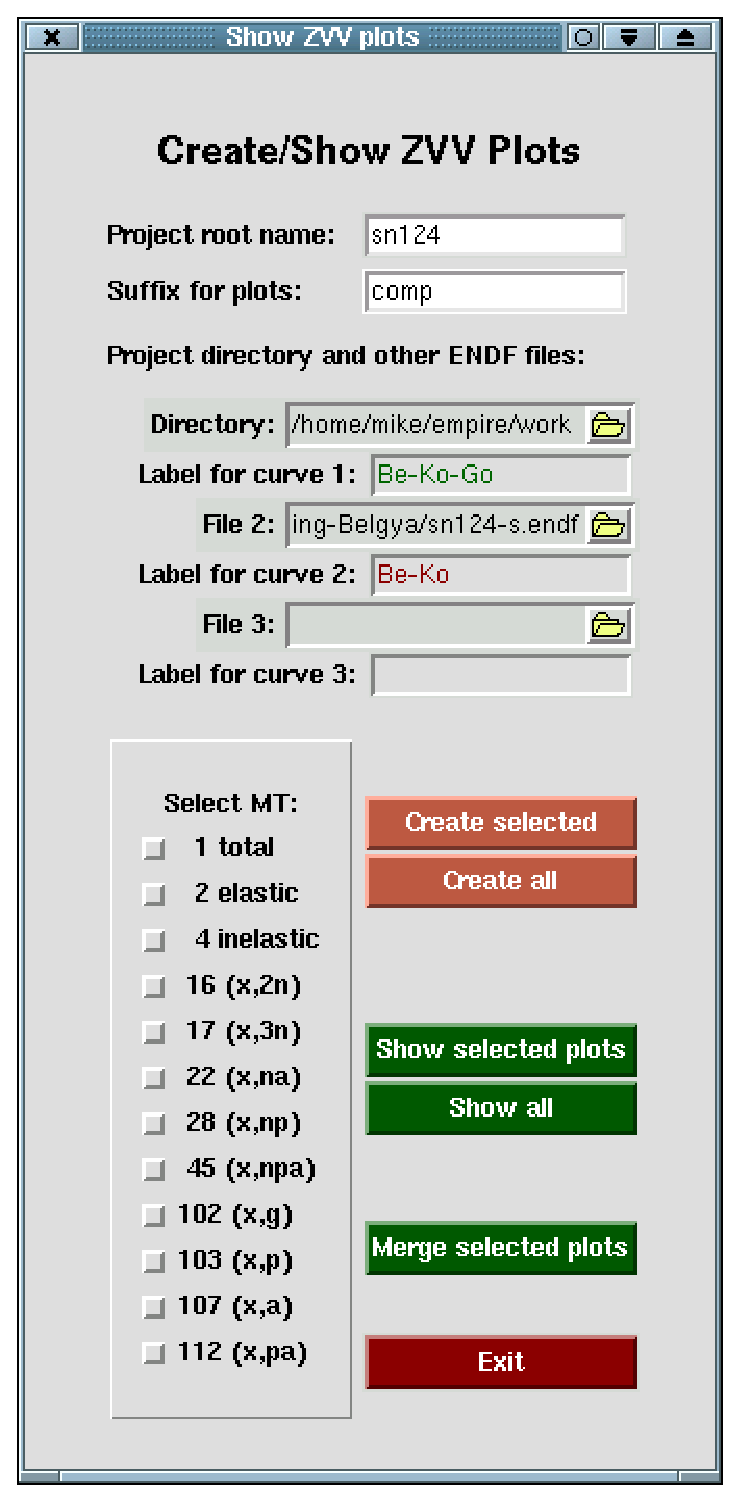
\includegraphics[height=0.3\textwidth,bb = 0 0 200 100, draft, type=eps]{ZVVGUI.eps}
\par\end{centering}

\caption{\label{fig:GUIZVV}Graphic User Interface to ZVView\index{ZVView}
to compare up to three calculations (or ENDF files) and merge different
reactions on a single ZVV plot.}

\end{figure}


As a rule, only the ENDF-formatted files can be plotted with PLOTC4\index{PLOTC4}
or ZVView\index{ZVView}. This choice is not only a matter of convenience
but was deliberately selected to validate the final (ENDF-formatted)
product. The only exception to this rule is provided by the \fbox{Create ZVV}
GUI button, which allows the user to construct and plot any excitation
function directly from the EMPIRE output. Hence, the user has to supply
a string which unambiguously identifies the cross section. The \emph{gawk}
script scans EMPIRE output (\emph{{*}.lst}) for the lines containing
the specified string and extracts a number (cross section) followed
by the \char`\"{}mb\char`\"{} string along with the respective incident
energy value. The results are sent to ZVView\index{ZVView} for plotting. 


\section{Plans for further development}

Following extensions are foreseen in future releases of the EMPIRE
code:

\begin{enumerate}
\item automatic adjustment of $\gamma$-strength functions to the observed
$\Gamma_{\gamma}$,
\item inclusion of isospin,
\item microscopic p-h level densities\index{p-h level densities} (routine
exists),
\item re-fit of level density systematics to the data recommended by RIPL-2,
\item Moldauer method for widths fluctuation correction, 
\item improved parametrization of the elastic enhancement factor,
\item further integration with the RIPL-2 library.
\end{enumerate}

\chapter{Working notes}


\section{Avoiding problems}

Consideration and observation of the following remarks will help to
avoid problems when running the EMPIRE code:

\begin{itemize}
\item Each modification of the EMPIRE input file ({*}.\emph{inp}) that involves
a change of projectile, target, or the number of emitted particles
must be followed by the execution of the \emph{clean} script in order
to remove input/output files that do not match the new case. One should
keep in mind that \emph{clean} will also remove all the files that
might have been modified manually (such as \emph{{*}.lev, {*}-omp.dir},
etc.). If these files are compatible with the new input and are to
be preserved they have to be renamed by adding a prefix before executing
the \emph{clean} script.
\item Any serious calculations should be preceded by a test run using FITLEV
set to a positive value in order to check the completeness of the
discrete level schemes and their consistency with the level densities\index{level densities}.
Such calculations should be repeated after each change of the input
file ({*}.\emph{inp}) that requires running the \emph{clean} script
(see above). Calculation times for such runs are very short. 
\item If the ENDF option is selected, the incident energies should be in
increasing order.
\item Log files \emph{{*}.war, {*}.x42c4\_errs} and \emph{empend.log} should
be checked for possible warnings and error messages.
\item The MSD\index{MSD}=2 option must be used with care. EMPIRE does not
check whether the existing output of ORION\index{ORION} (\emph{TAPE15})
is compatible with the currently executed case.
\item Irregularities in the excitation functions such as (n,2n) or (n,p)
are usually due to improper level density\index{level density} parametrization
(check cumulative plots of discrete levels) or to the overestimated
MSD\index{MSD} contribution (check response functions and ensure
that the levels to which they are adjusted are actually the collective
ones).
\item Irregularities in the increasing part of the excitation function for
inelastic scattering are usually due to insufficiently dense mesh
of incident energies.
\end{itemize}

\section{Fitting discrete levels}

Running EMPIRE with the FITLEV option is strongly recommended before
any cross section calculations are attempted. This allows a check
of whether the discrete level schemes for the involved nuclei are
complete and consistent with the level density\index{level density}
parametrization. If the whole package is properly installed, plots
of cumulative number of levels will be stored in the \emph{{*}-cum.ps}
file and can be inspected in the PostScript viewer (ghostview) by
clicking on the \fbox{Levels} button in the \char`\"{}Plots:\char`\"{}
section of the GUI. Two somewhat extreme examples of such plots are
shown in Fig. \ref{fig: badfit} and \ref{fig: goodfit}. Fig. \ref{fig: badfit}
demonstrates 10 levels in $^{96}$Pd, which could not be matched with
the level densities, which usually happens when the levels are over
extend. Then, levels that were not detected experimentally are missing
in the spectrum, and the resulting high energy end of the cumulative
plot is too low. Missing levels are more likely in the high-energy
region of the spectrum and reducing the number of levels considered
may restore agreement; neglecting the highest 4 levels in $^{96}$Pd
leads to a reasonable fit, as shown in the Fig. \ref{fig: goodfit}.
Graphical representation helps to identify the level at which cumulative
plot starts to bend, and levels lying above this point should be excluded
from consideration. One should edit .\emph{lev} file and decrease
$N_{max}$ parameters (6$^{th}$ entry in the first line of a given
isotope section) to remove levels in excess. The next step after the
modified \emph{{*}.lev} file is saved is to rerun the code and check
whether the applied cuts are sufficient. If this is not the case,
the whole procedure should be repeated and further levels removed.
Note, levels are only removed from the local file of the specific
case being calculated, and that \emph{Zxxx.dat} files in the parameter
library are not affected.

%
\begin{figure}[top]
\begin{centering}
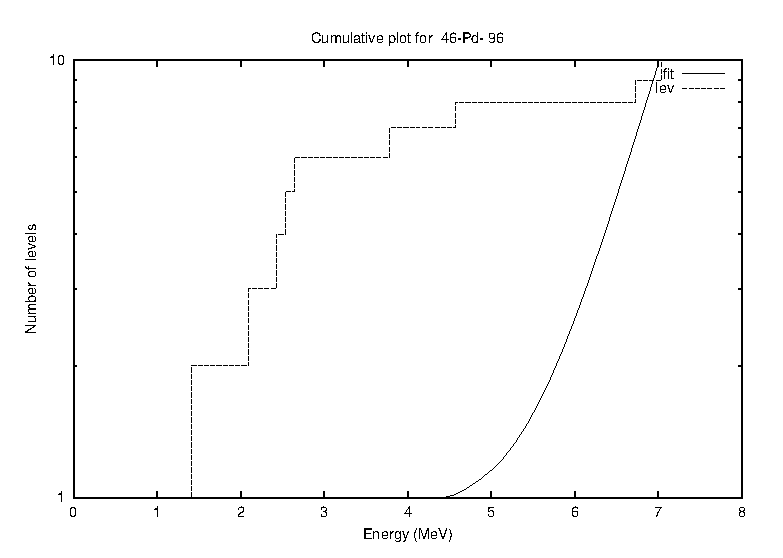
\includegraphics[width=0.7\textwidth,bb = 0 0 200 100, draft, type=eps]{bad-fitliv.eps}
\par\end{centering}

\caption{\label{fig: badfit} Cumulative plot of 10 discrete levels in $^{96}$Pd
which could not be reproduced by the level density\index{level density}
calculations (EMPIRE-specific level densities with default parametrization
were used).}

\end{figure}


%
\begin{figure}[top]
\begin{centering}
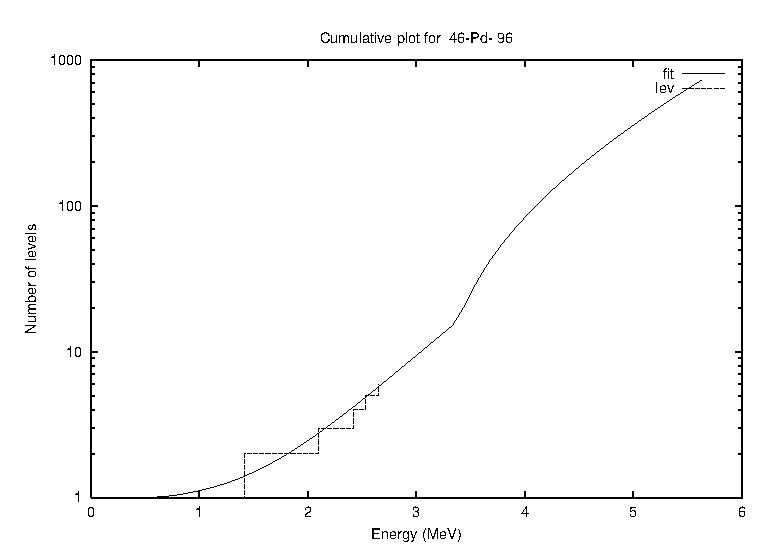
\includegraphics[width=0.7\textwidth,bb = 0 0 200 100, draft, type=eps]{good-fitliv.eps}
\par\end{centering}

\caption{\label{fig: goodfit}Same as Fig. \ref{fig: badfit} but after restricting
the fit to the first 6 levels only. Note the difference of two orders
of magnitude in the level densities\index{level density} around 6
MeV.}

\end{figure}


There are no restrictions on the contents of the input file ({*}.\emph{inp)}
used for displaying the cumulative plots except that the FITLEV record
must be included with VAL different from 0. Dispositions that do not
consider level densities are ignored as the code exits after the plots
are completed without performing any cross section calculations.


\section{Handling OM potentials}

Interface to the RIPL-2 optical model segment has been developed by
Capote. This interface allows the use of any type of Optical Model
Potential (OMP) contained in the library (including dispersive ones)
by specifying the OMP catalog number in the optional input (list of
available OMPs can be accessed from the EMPIRE GUI through the menu \fbox{Help}
$\Rightarrow$ \fbox{RIPL-omp})). The OMPOT record contains two numerical
values in addition to the usual keyword. The first value is the OMP
catalog number entered with a \textbf{negative} sign, which indicates
that the potential is going to be taken from RIPL\index{RIPL} rather
than from the internal sets coded in EMPIRE. The second value defines
the type of particle. For example,

\begin{labeling}{MMMMMMMMMMMM}
\item [{OMPOT~~~-401.~~~~~~1}] selects RIPL-2 Wilmore-Hodgson
global potential (RIPL-2 number 401) for neutrons,
\item [{OMPOT~~-4004.~~~~~~2}] selects RIPL-2 CC potential for
protons (to be used for $^{197}$Au only).
\end{labeling}
The code will create \emph{{*}-omp.ripl} file containing parameters
for the selected potentials for all nuclei and particles involved
in the calculations. This file can be edited in order to adjust OMP
parameters extracted from RIPL\index{RIPL}. RIPL Coupled-Channels
Optical Model Potentials (CC-OMP) include collective discrete levels
and related deformations, and thus the \emph{{*}-omp.ripl} contains
all information needed to run Coupled-Channel (CC) calculations. 

The ECIS03\index{ECIS} module, along with the RIPL\index{RIPL} interface,
bring into EMPIRE an easy access to a large number of optical model
potentials. However, the related input keywords (DIRECT, DIRPOT and
OMPOT) must be used with considerable care. In the following, we will
explain different combinations of these keywords, focusing on the
use of optical model parameters within EMPIRE. To this end we will
discuss several examples of neutron induced reactions on a spherical
nucleus ($^{54}$Fe) with dynamic deformation (vibrational case),
and on a deformed one ($^{153}$Eu) with static deformation (rotational
case). The general input file may contain the following lines:

\vspace{0.3cm}


\begin{flushleft}
\begin{tabular}{lrcl}
\texttt{DIRECT} & \texttt{x.} &  & ~call ECIS for CC, CC full or DWBA\tabularnewline
\texttt{DIRPOT} & \texttt{~~-xx.} &  & ~RIPL OMP for direct (inelastic) channel\tabularnewline
\texttt{OMPOT} & \texttt{~~-xx.} & \texttt{~~z} & ~RIPL OMP for particle z\tabularnewline
\end{tabular}
\par\end{flushleft}

\vspace{0.3cm}


In the following examples we use case-specific file names as created
when script or GUI modes are used to run the code. We recall that
the correspondence between the case specific names and those generated
by the code is the following:

\begin{labeling}{MMMMM}
\item [{\emph{{*}-omp.dir}}] $\Longleftrightarrow$ \emph{OMPAR.DIR }
\item [{\emph{{*}-omp.ripl}}] $\Longleftrightarrow$ \emph{OMPAR.RIPL}\index{RIPL} 
\item [{\emph{{*}-lev.col}}] $\Longleftrightarrow$ \emph{TARGET\_COLL.DAT }
\end{labeling}
\noindent with \char`\"{}{*}\char`\"{} standing for the actual root-name
of the file. 


\subsection{DWBA\index{DWBA} with RIPL OMP}

Apply the DWBA model to the spherical vibrational nucleus $^{54}$Fe.
Our goal is to perform calculations using default spherical RIPL potentials
for all channels, but including inelastic scattering calculated by
ECIS03\index{ECIS} with the DWBA\index{DWBA} option using RIPL spherical
OMP catalog number 10. The input file must contain two lines: 

\begin{labeling}{00.00.0000}
\item [{DIRECT}] 3. 
\item [{DIRPOT}] -10. 
\end{labeling}
Resulting OMP files: 

\begin{labeling}{00.00.0000}
\item [{\emph{{*}-omp.ripl}}] default RIPL OMP used for all the channels
in the HF\index{Hauser-Feshbach} calculations. 
\item [{\emph{{*}-omp.dir}}] spherical OMP employed in the DWBA\index{DWBA}
calculations of the inelastic scattering to collective discrete levels,
in this case RIPL\index{RIPL} OMP potential catalog number 10.
\end{labeling}
We can adjust the inelastic scattering cross sections in subsequent
runs by changing OMP inside the \emph{-omp.dir} file and/or by changing
dynamic deformations inside the \emph{{*}-lev.col} file (initial deformation
values are 0.15 for quadrupole and 0.05 for octupole vibrations).


\subsection{Coupled-Channels\index{Coupled-Channels} with RIPL spherical OMP}

Our goal is to perform calculations for $^{54}$Fe using default RIPL
potentials for all the channels, but including inelastic scattering
calculated by the ECIS03\index{ECIS} CC option using RIPL spherical
OMP potential catalog number 10. The input file must contain 2 lines: 

\begin{labeling}{00.00.0000}
\item [{DIRECT}] 1. 
\item [{DIRPOT}] - 10. 
\end{labeling}
Resulting OMP files: 

\begin{labeling}{00.00.0000}
\item [{\emph{{*}-omp.ripl}}] RIPL OMP used for all the channels in the
HF\index{Hauser-Feshbach} calculations. 
\item [{\emph{{*}-omp.dir}}] spherical OMP employed for the CC calculations
of the inelastic scattering to collective discrete levels, in this
case RIPL\index{RIPL} OMP catalog number 10.
\end{labeling}
We can adjust the inelastic scattering cross sections in subsequent
runs by changing OMP inside the \emph{{*}-omp.dir} file or by changing
dynamic deformations inside the \emph{{*}-lev.col} file.


\subsection{Coupled-Channels\index{Coupled-Channels} with RIPL Coupled-Channels
OMP for inelastic scattering}

We intend to perform calculations for $^{153}$Eu using RIPL spherical
potential catalog number 221 for all neutron channels (local potential
for $^{153}$Eu) except the inelastic channel, for which we are going
to calculate cross sections with the CC method using the RIPL\index{RIPL}
CC-OMP potential catalog number 2004. The input file must contain
3 lines: 

\begin{labeling}{00.00.0000}
\item [{DIRECT}] 1. 
\item [{DIRPOT}] -2004. 
\item [{OMPOT}] -221.~~~~~~~ 1
\end{labeling}
Resulting OMP files: 

\begin{labeling}{00.00.0000}
\item [{\emph{{*}-omp}.\emph{dir}}] deformed (CC) OMP employed for the
CC calculations of the inelastic channel, (RIPL\index{RIPL} potential
catalog number 2004 in this case (contains collective levels and respective
deformations)). 
\item [{\emph{{*}-omp.ripl}}] RIPL spherical OMP catalog number 221 used
in the HF calculations of neutron channels.
\end{labeling}
The inelastic scattering cross sections can be adjusted in subsequent
runs by changing OMP inside the \emph{{*}-omp}.\emph{dir} file or
by changing the static deformation of the ground state band inside
the same file. We are using a true CC-OMP from RIPL\index{RIPL} and
collective levels are stored together with the potential parameters
inside the \emph{{*}-omp}.\emph{dir} file. 


\subsection{Complete Coupled-Channels\index{Coupled-Channels} with RIPL CC OMP
for inelastic scattering}

Our aim is to performing exact calculations for $^{153}$Eu using
default EMPIRE potentials for all charged particle channels and the
RIPL spherical OMP catalog number 221 (local potential for $^{153}$Eu)
for all neutron channels except inelastic, for which we are going
to calculate cross sections and transmission coefficients consistently
using the CC method and the RIPL\index{RIPL} CC-OMP catalog number
2004. The input file must contain three lines: 

\begin{labeling}{00.00.0000}
\item [{DIRECT}] 2. 
\item [{DIRPOT}] -2004. 
\item [{OMPOT}] -221.~~~~~~~ 1
\end{labeling}
Resulting OMP files are: 

\begin{labeling}{MMMMMM}
\item [{\emph{{*}-omp.ripl}}] CC-OMP employed for the CC calculations of
the fusion and inelastic channels (RIPL\index{RIPL} CC-OMP number
2004 (contains collective levels and respective deformations)). In
addition, the file contains RIPL S-OMP number 221 employed for all
other neutron channels except inelastic. 
\item [{\emph{{*}-omp.dir}}] is not created since a true CC-OMP is used
consistently and all relevant parameters are contained in the \emph{{*}-omp.ripl}
file.
\end{labeling}
The inelastic scattering cross sections can be adjusted in subsequent
runs by changing either S-OMP inside the \emph{{*}-omp.ripl} file
or the static deformation of the ground state band inside the \emph{{*}-lev.col}
file (initial value is the experimental g.s. quadrupole deformation).
Note that the CC-OMP and the CC method are also used for the calculation
of the fusion cross section.


\section{Use of level densities}

The variety of nuclear level densities\index{level densities} available
in EMPIRE calls for additional guidance on their use. Only three options
are recommended: Empire-specific, Gilbert-Cameron (GC) and HF-BCS\index{HF-BCS};
all remaining options (such as ROCOL with level density parameter
\emph{a=A/8)} are included for comparison but their accuracy is much
lower than the three recommendations. The GC level densities, especially
when adjusted to known experimental data, may be the most accurate
at excitation energies up to the neutron binding and slightly above.
However, GC level densities do not lend themselves to extrapolation
to higher excitation energies and to nuclei far from the stability
line. Energy extrapolation in GC might be dangerous because of the
collective effects which are implicitly contained in the level density
parameter \emph{a}. While this can be an acceptable approximation
at low excitation energies for which level densities are fixed by
fitting experimental data (discrete levels and neutron resonance spacings),
there is no physical justification for extending such a treatment
to higher energies. In fact, collective effects, as implicitly accounted
for in the GC approach, increase exponentially with excitation energy
instead of decreasing and eventually disappearing. In this respect,
EMPIRE-specific and microscopic HF-BCS\index{HF-BCS} densities behave
properly and should be preferred at excitation energies well above
neutron binding. 

EMPIRE-specific level densities\index{level densities}, in addition
to explicit treatment of the collective effects and their damping,
also include the effects of dynamic deformation, which is induced
by the rotation of a nucleus at high spin. This deformation affects
level densities through the modification of nuclear moments of inertia.
The yrast line is taken into account by setting level densities to
zero whenever the thermal energy available for single particle motion
is negative. Thermal energy is calculated as the difference between
the total excitation energy and the energy needed for rotation. Spin
and energy ranges are also formally unlimited in the EMPIRE-specific
level densities. These features make the approach particularly suited
for the Heavy Ion and high-energy nucleon-induced reactions. On the
other hand, EMPIRE-specific level densities are fitted to the experimental
data in a manner similar to the GC, suggesting that their predictions
at low energies should be comparable to those of GC or even better
due to the use of the BCS\index{BCS} model below critical energy.
Therefore, EMPIRE-specific level densities\index{level densities}
are generally recommended, and are used as a default in the EMPIRE.

However, EMPIRE-specific level densities suffer the same uncertainty
as GC when extrapolating from the stability line, because both relay
on experimental parameterization of the level density parameter \emph{a},
which is only possible for stable or close to stable nuclei. For nuclei
far from the stability line, the HF-BCS\index{HF-BCS} densities based
on realistic schemes of single particle levels offer higher reliability.
The physics involved in this approach is clearly superior to the treatment
used in the two models discussed above, which makes HF-BCS densities
more suitable for extrapolation. In addition, the tabulated values
provided by Goriely for RIPL\index{RIPL}-2 and available in EMPIRE
were adjusted to the same experimental data as the other two phenomenological
approaches. Therefore, results of the HF-BCS model at low energies
should not differ significantly from those provided by the GC or EMPIRE-specific
models. Comparisons of cross section calculations for about 300 reactions
on targets from $^{40}$Ca to $^{208}$Pb show that microscopic level
densities\index{level densities} can compete with the phenomenological
ones to the extent that makes them the preferred choice far from the
stability line. On the other hand, one should keep in mind that tables
of level densities are limited to excitation energies below 150 MeV
and spins up to 30$\hbar$, which prevents their use for the Heavy
Ion induced reactions well above the Coulomb barrier. 


\section{Parameter tuning}

The parameter libraries and internal systematics contained in the
EMPIRE code perform reasonably well in reproducing cross sections
for major neutron induced reactions up to 20 MeV. However, one can
not expect that global parametrization will provide perfect fits to
all channels and at all incident energies. Weak reaction channels
may differ substantially from the experimental data. In view of the
uncertainties associated with the model parameters, certain adjustments
were made in order to fit measured cross sections. Guidance is given
below on parameter tuning, indicating the most sensitive methods and,
if possible, describing the effect of their modification.

It is strongly recommended that various available options in the code
are exploited before any attempt is made to change the parameters.
This guarantees that physically meaningful parameters are used. For
example, the user may try different optical model potentials, various
formulations and/or parameterizations of level densities\index{level densities}
and eventually different preequilibrium models. These attempts should,
at least, provide the user with the best starting point for parameter
adjustment. We note that various options may provide very different
results as illustrated by the following three sets of calculations:

\newpage

\begin{labeling}{00.00.0000}
\item [{standard}] Wilmore-Hodgson S-OMP for neutrons and Becchetti-Greenlees
for protons, EMPIRE-specific level densities with internal systematics,
and discrete levels up to N$_{max}=10$ (note that in EMPIRE-2.19
Koning-DeLaroche potential is a standard),%
\begin{figure}[top]
\begin{centering}
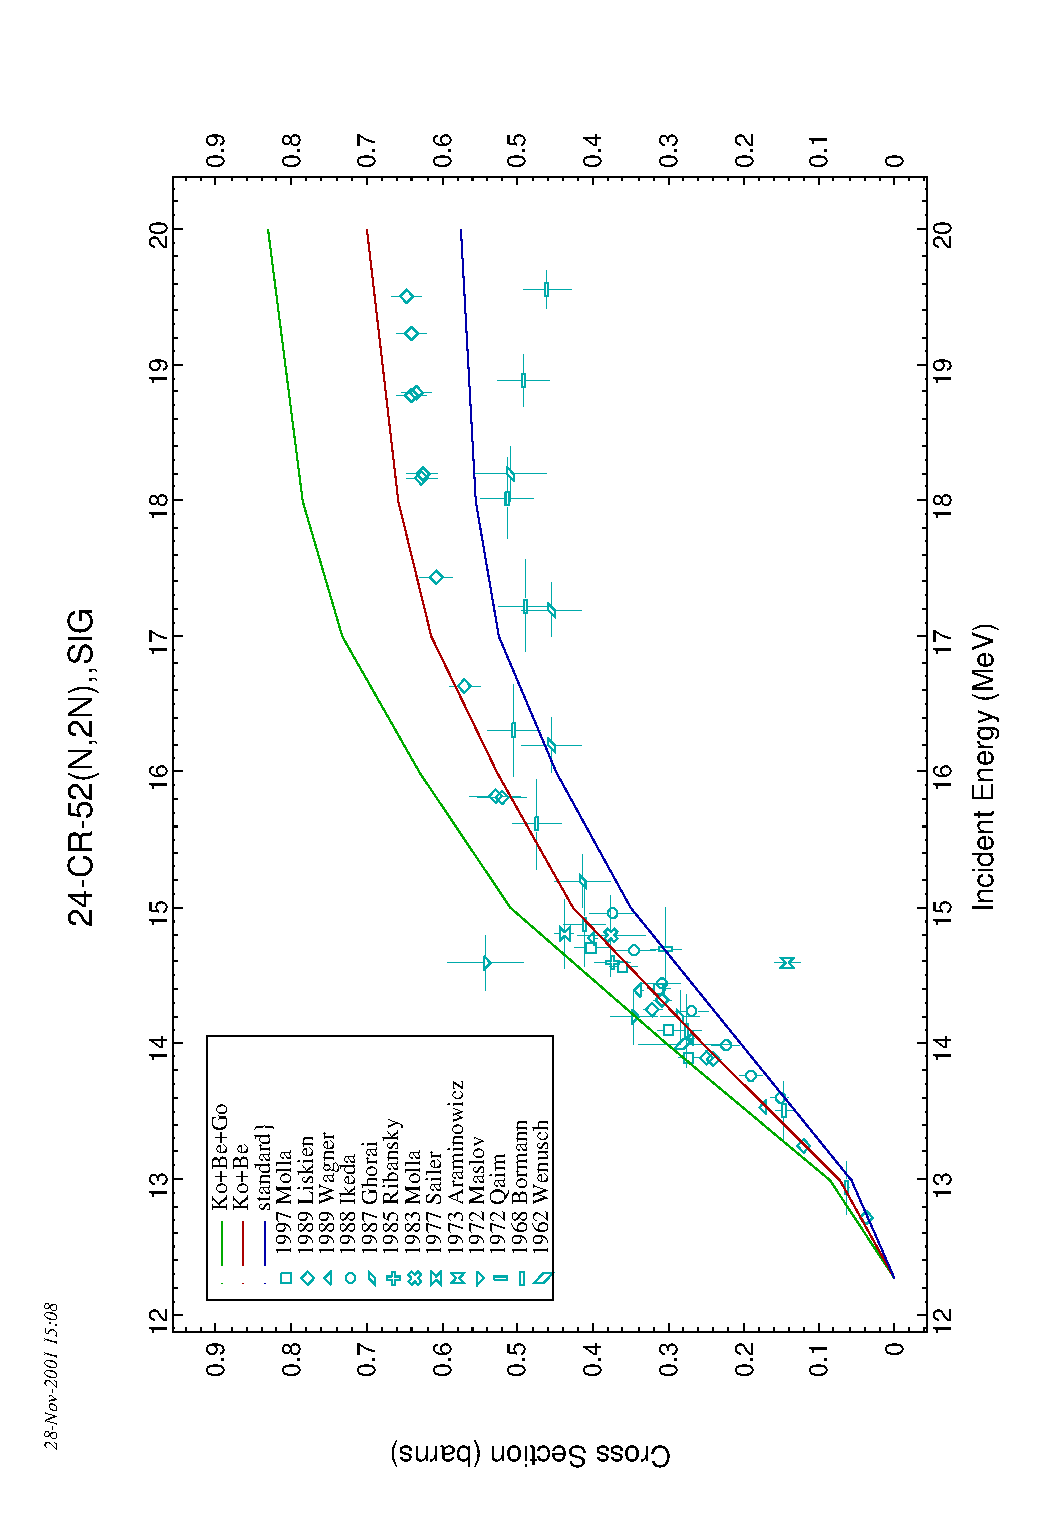
\includegraphics[width=0.7\textwidth,keepaspectratio,angle=-90,bb = 0 0 200 100, draft, type=eps]{cr52n2n.eps}
\par\end{centering}

\caption{\label{complot1}Comparison of experimental data with results calculated
using three sets of parameters for the $^{52}$Cr(n,2n) reaction (see
text).}

\end{figure}

\item [{Ko-Be}] Koning-DeLaroche S-OMP for neutrons and protons, discrete
levels up to the N$_{max}$ recommended by RIPL-2 (limited to 40 by
the ENDF-6 format), and EMPIRE-specific level densities,
\item [{Ko-Be-Go\label{Ko-Be-Go}}] as above but using HF-BCS\index{HF-BCS}
microscopic level densities\index{level densities}\cite{HFBCS} instead
of the EMPIRE-specific ones.
\end{labeling}
Fig. \ref{complot1}, \ref{complot2} and \ref{complot3} show comparison
of the results obtained using the above sets of parameters in three
sample cases. Differences of a factor of 2 are observed, and therefore 

%
\begin{figure}[top]
\begin{centering}
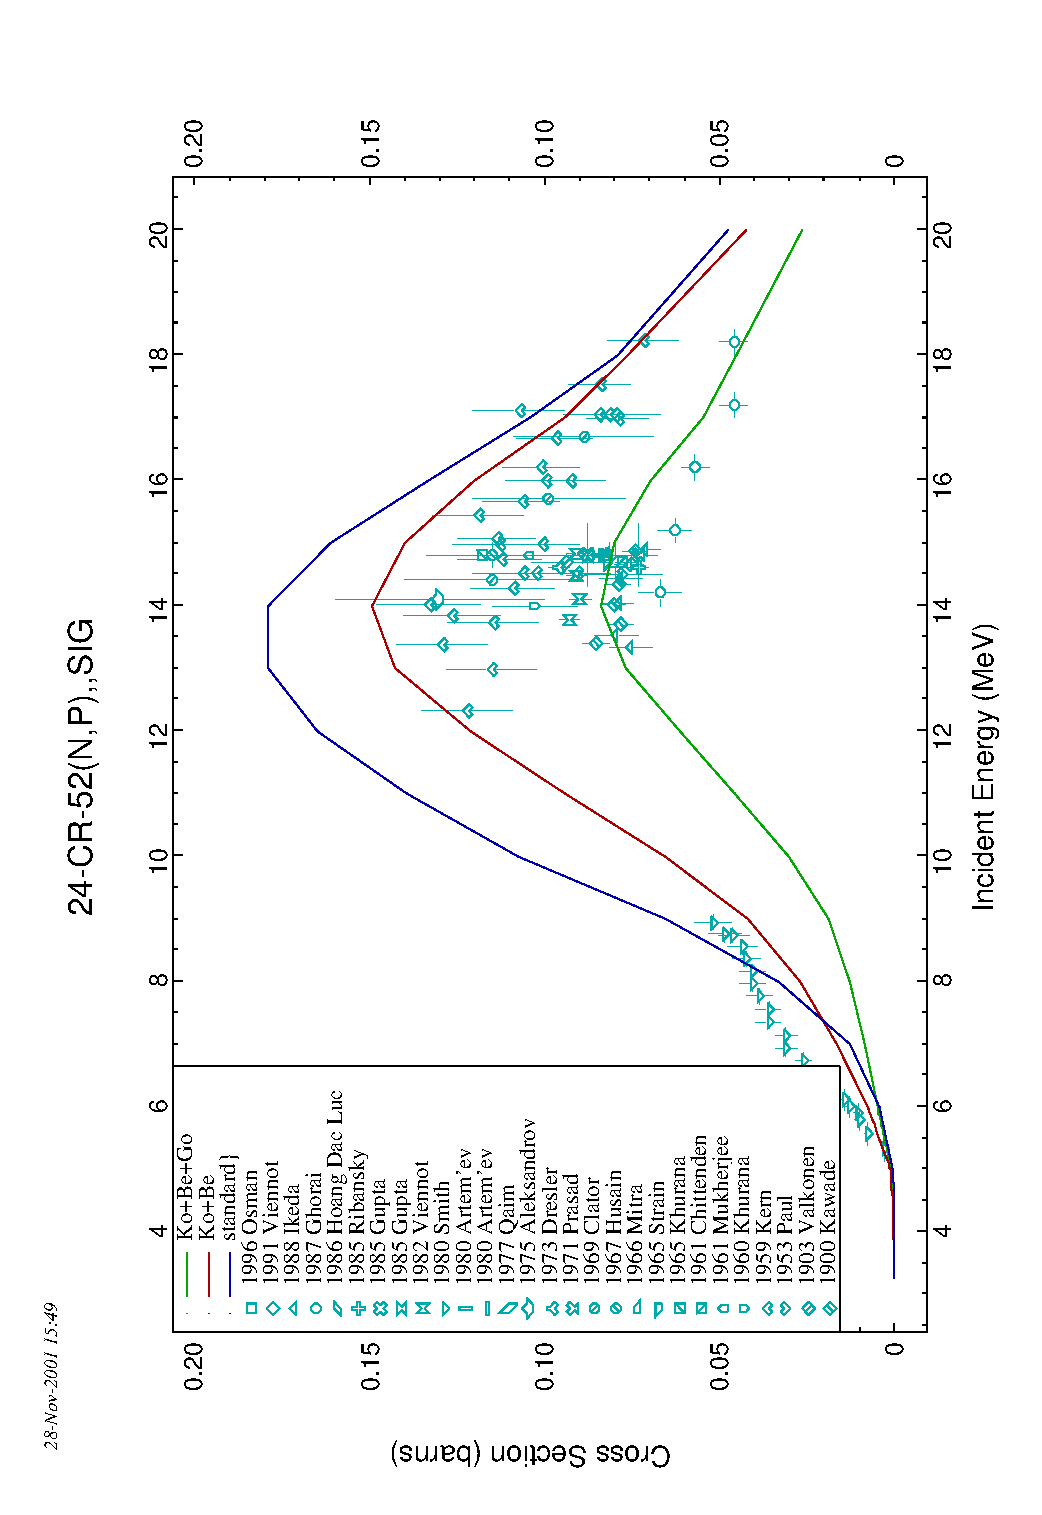
\includegraphics[width=0.7\textwidth,keepaspectratio,angle=-90,bb = 0 0 200 100, draft, type=eps]{cr52np.eps}
\par\end{centering}

\caption{\label{complot2}Comparison of experimental data with results calculated
using three sets of parameters for the $^{52}$Cr(n,p) reaction (see
text).}

\end{figure}


changing the default options may considerably improve the comparison
with experimental data. However, this approach may still not be sufficient
in some cases, and the next step would be to determine which reaction
mechanism is most likely to be responsible for the disagreement, remembering
that neutron capture below 10 MeV and the low energy part of the particle
spectra are essentially due to Compound Nucleus decay. The high energy
part of particle spectra is dominated by the preequilibrium emission,
and population of the collective discrete levels in inelastic scattering
arises mainly from the direct reactions. We also note that at incident
energies below 50 MeV the multiple-chance preequilibrium emission
is rather small and multiple particle emission is governed by the
statistical decay. The list below should help pinpoint the mechanism
that might be causing a problem:

%
\begin{figure}[top]
\begin{centering}
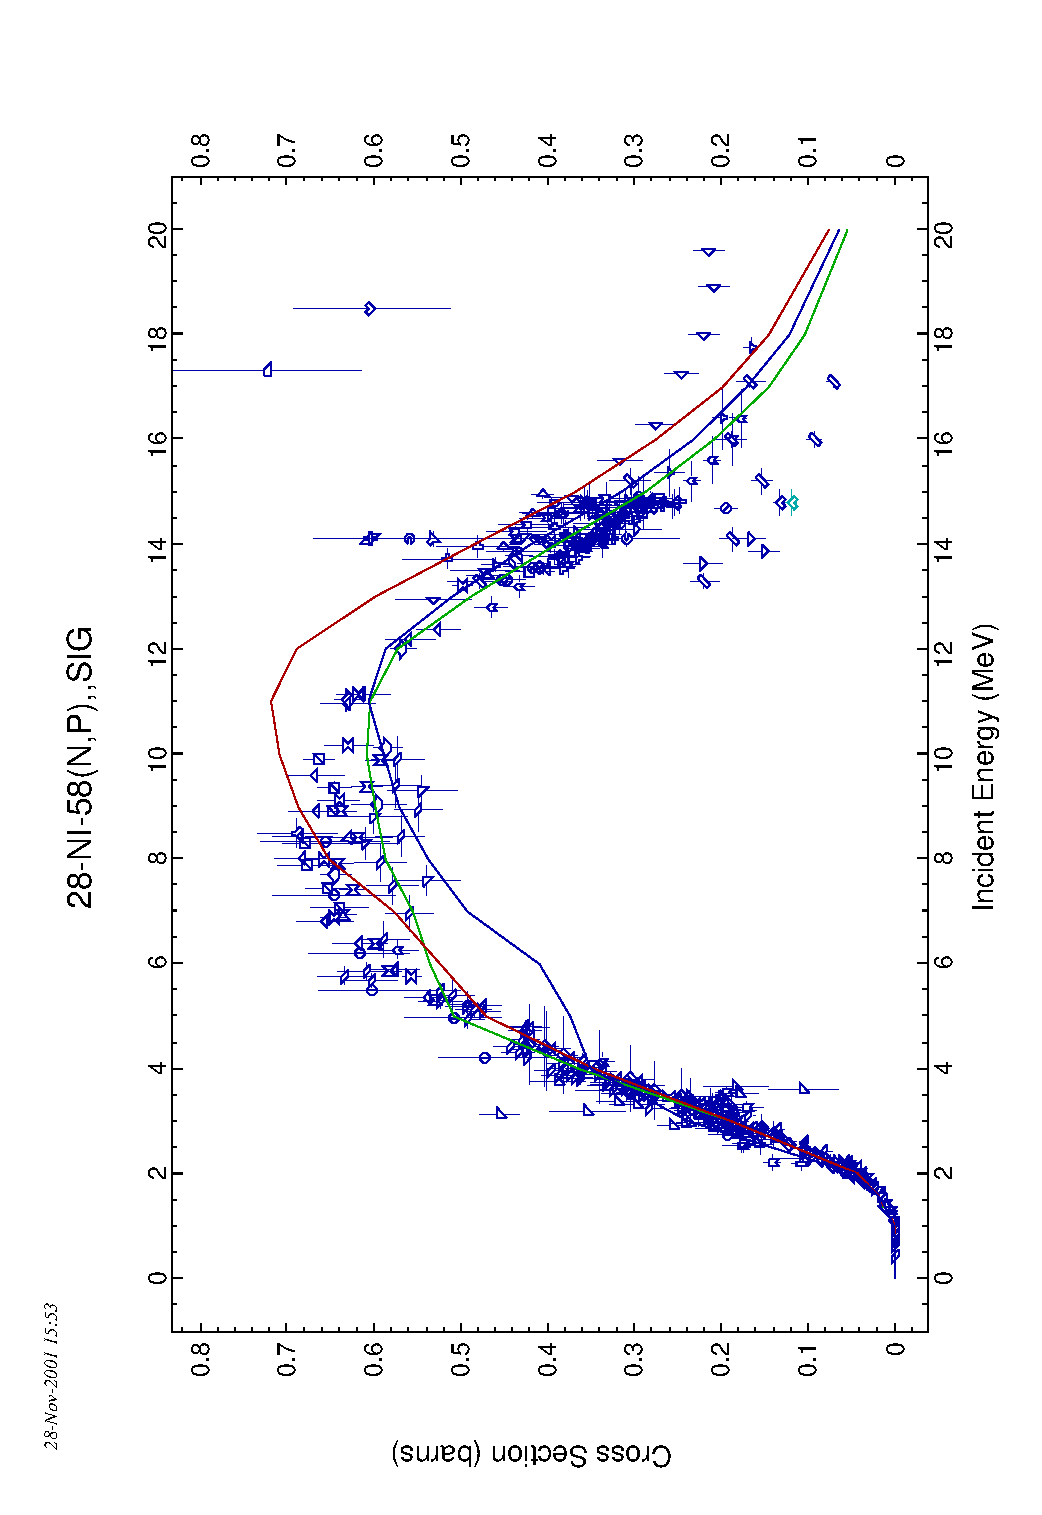
\includegraphics[width=0.7\textwidth,keepaspectratio,angle=-90,bb = 0 0 200 100, draft, type=eps]{ni58np.eps}
\par\end{centering}

\caption{\label{complot3}Comparison of experimental data with results calculated
using three sets of parameters for the $^{58}$Ni(n,p) reaction (see
text).}

\end{figure}


\begin{itemize}
\item \textbf{Nucleon spectra at high ejectile energies underestimated (overestimated)}
- these are usually related to the underestimated (overestimated)
preequilibrium emission.
\item \textbf{Tails of the inelastic scattering cross sections underestimated
(overestimated)} - again caused by too low (too high) preequilibrium
contribution. 
\item \textbf{Inelastic cross sections to discrete levels} \textbf{underestimated
(overestimated)} - lack of or too low (too high) contribution from
the direct reactions is the most likely reason. In case of under-estimation,
user should ensure that Coupled-Channel or DWBA\index{DWBA} option
is turned on (DIRECT=1, 2, or 3). Generally, the Coupled-Channel option
will provide higher cross sections than DWBA.
\item \textbf{Capture cross sections below 10 MeV} \textbf{underestimated
(overestimated)} - as mentioned before, the Compound Nucleus is responsible.
The discrepancy might be traced to $\gamma$-ray strength function
being too low being too low (too high) or to the ratio of level densities\index{level densities}
in the daughter nuclei and the Compound Nucleus being too low (too
high) ($\rho_{n}/\rho_{CN}$ - note that the neutron channel is usually
the main competitor). 
\item \textbf{Capture cross sections above 10 MeV} \textbf{underestimated}
- be sure that the exciton model DEGAS\index{DEGAS} is turned on.
The preequilibrium emission of $\gamma$s (or the Direct-Semidirect
mechanism) is responsible for more than 90\% of the capture cross
section in this energy range.
\item \textbf{Cross sections} \textbf{underestimated (overestimated)} \textbf{in
all channels} - can be traced to an inadequate optical potential that
provides too low (too high) absorption cross section.
\item \textbf{Wrong total cross section} - obviously an inadequate optical
potential. 
\item \textbf{Wrong angular distributions for elastic scattering} - again
would assume an inadequate optical potential to be the main reason.
At low energies where few inelastic channels are open, there might
be a non-negligible contribution from the symmetric compound elastic,
which could be affected by the wrong $\rho_{n}/\rho_{CN}$ ratio.
\item \textbf{Cross sections for the $\alpha$-channel} \textbf{underestimated}
- for nuclei with masses larger than about 100, the discrepancy is
not due to wrong parameters but to the lack of a preequilibrium emission
of clusters in the present version of EMPIRE. One may compensate for
this deficiency by increasing level densities\index{level densities}
in the residue after $\alpha$ emission or by increasing the diffuseness
of the optical model potential for $\alpha$-particles. However, the
resulting parameters will be unphysical. Such an intervention may
only be justified for lighter nuclei, for which preequilibrium emission
of $\alpha$-particles is relatively unimportant. 
\item \textbf{Fission cross sections} \textbf{underestimated (overestimated)}
- for neutron induced fission, the current fission model coded in
EMPIRE is too crude. One may try to cure the problem by decreasing
(increasing) the fission barrier or increasing (decreasing) level
densities at the saddle point, but this should be considered as an
arbitrary fitting exercise without much physical meaning. Tuning fission
cross sections in the HI induced reactions will be discussed later
on.
\item \textbf{Excitation functions shifted in energy} - for nuclei far from
the stability line (typical for HI induced reactions), this effect
can be traced to incorrect binding energies (masses). A modest change
of binding energies (of the order of 0.5 MeV) can be justified as
being within the uncertainty of the theoretical masses. However, this
argument does not hold for nuclei close to the stability valley since
experimental nuclear masses are known with a rather high accuracy.
\item \textbf{Structure in the continuum part of the inelastic scattering
spectrum \char`\"{}out of phase\char`\"{}} - this structure originates
from the MSD\index{MSD} contribution. When the spectrum does not
match experiment, the user may attempt to tune calculations by changing
the positions of collective levels to which the response functions
are fitted.
\item \textbf{Double-differential spectra for inelastic scattering to continuum
at small angles (<40$^{o}$) underestimated} - MSD\index{MSD} mechanism
is responsible for the major part of the cross section in this range.
Choosing the compressional form factor for the $l=0$ transfer (default
is the surface form factor) should bring substantial improvement.
In fact, from the physical standpoint this \emph{is} the factor that
should be used for the $l=0$ transfer. The different default is being
used due to the numerical instabilities that happen occasionally when
this physically-correct option is selected. 
\item \textbf{Wrong ratio between two competing channels (e.g., $\sigma$(n,n)
/$\sigma$(n,p))} - at low incident energies this ratio is governed
by the Compound Nucleus decay and may be distorted by an inappropriate
ratio of level densities\index{level densities} in the two competing
channels. Actually, the cross section ratio is approximately proportional
to the level density ratio in the respective residual nuclei. Also,
the optical model potential may have a significant effect. At higher
incident energies, the preequilibrium contribution starts to play
a role, and a reference for one of the preequilibrium channels may
provide a solution.
\item \textbf{Wrong slope of the increasing part of the excitation function}
- a crucial role is played by the discrete levels in the residual
nucleus and the optical model potential (transmission coefficients),
of which the discrete levels are easier to control. Changing the number
of accepted levels may effectively increase or decrease the available
phase space for the particular decay mode.
\item \textbf{Production of residues in HI induced reaction underestimated
(overestimated)} - for lighter nuclei in which the fission channel
is not dominant, the fusion cross section might be too small (or too
big). Competition between fission and particle emission may constitute
an additional source of error for the highly fissile (heavy) nuclei.
In such a case, decreasing (increasing) strength of the fission channel
is usually an effective way of increasing (decreasing) residue production. 
\end{itemize}
The mechanisms and parameters that are expected to be the most important
and effective in solving a particular problem have been noted in the
above discussion. However, we are always dealing with a complicate
interplay of different factors and in some cases the major sources
of error may differ from those indicated. However, the user should
be able to identify the most critical reaction mechanism or a key
input quantity in most cases, and be able to avoid a random search
for optimal parameters. 

So far we have discussed the symptoms and possible reasons for operational
problems. Knowing the disease, we should now look for the most appropriate
treatment. We will indicate those input parameters to which particular
models or input quantities (such as fusion, level densities and\index{level densities},
$\gamma$-ray strength functions) are most sensitive. However, parameters
not mentioned below may also influence the results. Generally, their
effect should be less pronounced but they might become one of the
key players in particular situations. In addition, these assessments
are complicated and most of the parameters are correlated; for example,
deficiencies in one parameter can be compensated by a change in another
leading to unrealistic values. Therefore, it is important to understand
the physical reason for a discrepancy and proceed accordingly, and
to fit all available observables rather than a single cross section.
Such an approach increases the user's confidence in the final results.
Finally, fitting a single experimental point that differs dramatically
from the calculated value can be dangerous, especially when the exercise
involves a strong channel. The experimental point might simply be
wrong. Such cases are known in the EXFOR library, either because of
an erroneous experiment or a compilation error. In particular, if
the experimental data fall well below the calculated cross section,
the user should check whether the measurement concerned the total
cross section for the reaction channel or the cross section to the
isomeric or ground state.

In the discussion that follows, we group parameters according to the
reaction mechanism or input quantity to which they are relevant, and
refer to them by keywords defined in the input description (see Section
\ref{sec: input}). 


\subsubsection*{Fusion}

We have to distinguish between Heavy Ion and Light Ion (A<5) of nucleon
induced reactions. Heavy Ion induced reactions:

\begin{labeling}{00.00.0000}
\item [{FUSRED}] scales calculated fusion cross section with an arbitrary
factor to set the parameter directly to the desired value, but lacks
any physical significance and predictive power. Should be used as
the last resource unless the fusion cross section is known from a
more microscopic model or experiment. 
\item [{BFUS}] Fusion barrier height in the distributed barrier model $B_{fus}$
(Eq. \ref{distbarr}) is by default calculated by the CCFUS\index{CCFUS}
and used for the HI induced reactions only. Even a slight decrease
of the barrier height can produce a considerable increase of the fusion
cross section (and vice versa) when the incident energy (in CM) is
close to the barrier height. This effect tends to disappear at higher
incident energies. 
\item [{SIG}] SIGMA in the distributed barrier model (Eq. \ref{distbarr})
is by default set to $0.05B_{fus}$. Increase of SIGMA will also increase
the fusion cross section. Similarly to BFUS, the effect is most pronounced
at low energies and tends to disappear at higher values.
\item [{EXPUSH}] Extra-push energy (default value is 0) is very effective
at decreasing the HI fusion cross section when increased. Physically
justified for a fusion of massive systems.
\item [{CRL}] Critical \emph{l}-value for the HI fusion (Eq. \ref{Tlfus})
sets fusion cross section to the required value - much like FUSRED.
\item [{DFUS}] Diffuseness in the transmission coefficients of HI fusion
(Eq. \ref{Tlfus}) does not change the fusion cross section, but defines
the spin distribution. Larger DFUS, the higher the spins populated,
and this effect may contribute to an increase of the fission cross
section and resulting reduction in the evaporation residues.
\end{labeling}
Most of the parameters discussed above concern HI induced reactions.
There are fewer possibilities for nucleons as the fusion (or absorption)
cross section is calculated using the optical model. Users may try
different parameterizations available in the RIPL\index{RIPL} library
or internal OMP systematics. If this fails, increasing the imaginary
part of the OMP will increase the absorption cross section. However,
users are advised that blind modification of the OMP can easily produce
physically unrealistic results. 


\subsubsection*{Coupled-Channels\index{Coupled-Channels} (ECIS\index{ECIS})}

CC calculations are most sensitive to the deformations of collective
levels, which can be adjusted by editing the \emph{{*}-lev.coll} file
(see Section \ref{lev-coll}). Actually, if the collective levels
are selected internally rather than taken from the RIPL\index{RIPL}
library along with the CC optical model potential, these deformations
\emph{should} be adjusted. The code sets them by default to the g.s.
deformation for the rotational model and to the arbitrarily fixed
values for the vibrational model. These values can only be considered
as a first guess. Increasing the band deformation for the rotational
model or dynamic deformations for the vibrational model results in
an increase of the calculated direct cross sections (opposite is true
if the deformations are decreased).

Adding more collective levels to the \emph{{*}-lev.coll} file will
generally increase the total direct cross section, and may result
in a substantial increase of the cross section to the introduced levels.
Generally, the overall effect is not very significant as high energy
levels are usually only weakly coupled. Substantial increase of the
direct cross section, especially for the highly deformed nuclei, can
be achieved by using the CC approach instead of DWBA\index{DWBA}.
As a rule, CC model \emph{should} be the preferred choice in such
cases.

Obviously, the cross sections calculated with the CC model are sensitive
to the OMP. The effect might be considerable but is difficult to predict
due to the large number of parameters involved. Generally, deeper
imaginary part of the OMP (especially the imaginary surface component)
will result in the higher cross sections.


\subsubsection*{Multi-step Direct\index{MSD}}

The microscopic character of the MSD\index{MSD} model limits the
possibilities of influencing the results compared with the classical
models (such as the exciton model). A certain degree of flexibility
is provided by the pairing gap parameters (GAPP for protons and GAPN
for neutrons). The dependence is non-linear, and it is difficult to
predict the impact of any change. MSD\index{MSD} results are slightly
more sensitive to the EFIT parameters, which define the energies of
the collective levels to which response functions for different multipolarities
are fitted. Again, due to the non-linearity, the results of the change
are hard to predict, the effect has an oscillating character. However,
on average, decreasing the EFIT value for a given multi-polarity results
in an increase in strength for the $l$-transfer under consideration
and a higher MSD\index{MSD} cross section. We stress again that EMPIRE
sets EFIT values internally to the energy of the lowest discrete level
which can be coupled to the ground state with a given $l$ transfer
(except $l=0$ transfer for which the self-consistent value is taken
by default). This assignment might be erroneous if there happens to
be a non-collective and low energy level with a suitable spin. In
such a case, the EFIT value should be corrected manually by entering
the EFIT keyword with the proper energy of the true collective level.
Modifications in the EFIT values will generally affect the structure
observed in the MSD\index{MSD} spectra by shifting maxima to different
energies, and the user is advised to try first the self-consistent
values for EFIT before attempting any arbitrary modifications.

Substantial increases in the MSD\index{MSD} contribution at \emph{forward
angles} can be obtained by switching to the compressional form factor
for the $l=0$ transfer (COMPFF=1). As already mentioned before, this
option is physically sound and strongly recommended.

The last resource involves multiplying the response function by an
arbitrary factor through the RESNOR entry. Factors larger than 1 will
increase MSD cross sections, and values smaller than 1 will reduce
it. This procedure has no physical meaning and may eventually lead
to the MSD emission being larger than the absorption cross section. 


\subsubsection*{Multi-step Compound\index{MSC} }

The most significant MSC\index{MSC} contribution to the nucleon spectra
is located between the Compound Nucleus (low energies) and the MSD\index{MSD}
contributions (middle-high energies). MSC mechanism accounts for about
20-30\% of the total emission at incident energies close to 10 MeV
and decreases with the increasing incident energy. Therefore, one
should not expect too much from tuning this mechanism. Similarly to
MSD, the user's freedom to modify MSC is rather limited. The parameters
that have the largest effect are as follows:

\begin{labeling}{00.00.0000}
\item [{GDIV}] Single particle level densities defining particle-hole level
densities\index{p-h level densities} in MSC\index{MSC} set to A/13
by default. Increasing (decreasing) GDIV will result in a higher (lower)
MSC cross section. Note that increasing GDIV is justified for nuclei
close to the magic numbers, as their level densities are significantly
lower. 
\item [{TORY}] Ratio of the cross sections for unlike and like nucleon-nucleon
interaction (e.g., $\sigma_{np}/\sigma_{nn}$). Can be used for adjusting
the relative share between neutron and proton emission. The default
value of 4, as derived from the free nucleon scattering, is generally
accepted, although some doubts have been expressed as to whether the
free scattering value should be applied to the scattering inside nuclear
matter. Increasing (decreasing) this parameters will favor (suppress)
the charge exchange channel.
\item [{D1FRA}] Ratio of the GDR spreading width to the total GDR width
(default: 0.8) is relevant to $\gamma$-emission only. While there
is not much room for increase, decreasing the ratio will also reduce
the already low $\gamma$-emission through the MSC\index{MSC} mechanism.
\end{labeling}

\subsubsection*{Exciton model (DEGAS\index{DEGAS}) }

The above discussion of the GDIV parameter also applies to the exciton
model calculations in the neutron channel. DEGAS also offers the possibility
to vary independently the single particle level density in the proton
channel, which allows modifications to the neutron/proton emission
ratio. By default, both single particle densities are taken to be
equal. 


\subsubsection*{Level densities}

The Hauser-Feshbach results are very sensitive to the level densities\index{level densities},
and more precisely to their ratio in the neighboring nuclei. Generally,
changing level densities is the most effective way of adjusting cross
sections. As mentioned at the beginning of this Section, various formulations
of the level densities provided in EMPIRE should be considered with
their default parameterization first. Only if this exercise does not
produce sensible results should the user attempt to vary the model
parameters. The three recommended and most accurate models are (i)
EMPIRE-specific, (ii) Gilbert-Cameron, and (iii) HF-BCS\index{HF-BCS}.
All of them are fitted to match the discrete levels. While the pre-calculated
HF-BCS level densities can not be modified, EMPIRE and Gilbert-Cameron
offer more significant flexibility. First of all, they are affected
by the number of discrete levels in the calculations (it is assumed
that cumulative plots had already been checked for consistency using
the FITLEV option). Generally, adopting fewer levels increases the
level densities between the last discrete level and neutron binding
energy, and considering more levels tends to decrease level densities\index{level densities}
in the same region (see Fig. \ref{fig: badfit} and \ref{fig: goodfit}).
However, this general statement may not hold in cases with strong
irregularities in the cumulative plots. Extending the discrete level
scheme too far involves a risk of including the region with missing
levels which would lead to an unphysical reduction of level densities.
The new RIPL-2 library of discrete levels contains estimates of the
completeness of the scheme (N$_{max}$), which is used by EMPIRE as
a default. These values have been compared with the EMPIRE level densities
(i) and (ii) and were found to be compatible in about 75\% of cases.
The user should decrease N$_{max}$ in the remaining 25\%. If this
reduction is insufficient the discrete level region may extend too
far. Another extreme involves too few levels, in which there is a
risk of fitting level densities to a bunch of collective levels that
are shifted toward lower energies because of their collective nature.
The resulting level densities might be considerably overestimated. 

Changing the level density models and the number of discrete levels
may fail, and the user may be forced to adjust the level density parameters
themselves. Depending on the model there are different possibilities
for explicit adjustment of level density parameters. EMPIRE-specific
level densities: $a$-parameter is energy and spin dependent, and
can not be read as a single input entry. However, there is a possibility
of applying a factor (ATILNO) to the asymptotic value of the $a$-parameter,
which is equivalent to multiplying each $a$-parameter (larger $a$
values correspond to larger level densities\index{level densities}).
There are no other parameters in the EMPIRE-specific level densities
that can be controlled from the input. The Gilbert-Cameron level densities
offer more flexibility: all of the parameters can be specified in
the input file. However, it is a responsibility of the user to ensure
that these parameters are internally consistent (i.e., fulfill matching
conditions and fit discrete levels). A much safer approach involves
the introduction of the $a$-parameter and one other ($U_{x},\, E_{o},$
and $T$), and allows the code to take care of the internal consistency.
As usual, level densities increase with $a$-parameter. The constant
temperature component (low energy) of the level densities increases
with decreasing $T$ and $E_{o}$, and higher values of $U_{x}$ correspond
to higher level densities\index{level densities}. Finally, within
the Gilbert-Cameron approach coded in EMPIRE, there are three built
in systematics for $a$, that can be selected with the GCROA keyword:

\begin{labeling}{00.00.0000}
\item [{GCROA}] = ~0 Ignatyuk systematics,\\
= -1 Arthur systematics,\\
= -2 Ilijnov systematics (default).
\end{labeling}

\subsubsection*{Fission}

Fission can be scaled quite effectively with a number of parameters,
especially in the HI induced reactions. The reduced dissipation coefficient
$\beta_{v}$ is controlled by the keyword BETAV, and decreases the
fission channel when moved further out from the 3.2 value (corresponding
to $\beta_{v}=3.2\cdot10^{-21}\, s^{-1}$), separating the under-damped
and over-damped motion. All remaining input parameters affect directly
(e.g., QFIS) or indirectly the height of the fission barrier, and
can be divided into those that control shell correction damping with
spin and temperature and those that modify the fission barrier by
adding a Gaussian centered at a certain spin. All of them are listed
below: 

\begin{labeling}{00.00.0000}
\item [{QFIS}] Liquid drop fission barrier multiplier. QFIS>1 decreases
fission channel. 
\item [{SHRJ}] Shell correction to fission barrier is damped to 1/2 (Eq.
\ref{BfJfade}) at the spin defined by SHRJ. For negative shell corrections,
lowering SHRJ will increase the fission channel, at least at sufficiently
high incident energies. Opposite is true for positive shell corrections.
\item [{SHRD}] Diffuseness of the shell correction damping (Eq. \ref{BfJfade}).
The size and sign of the effect depend on the actual spin population
of the fissioning nucleus. 
\item [{TEMP0}] Temperature at which temperature-damping of the shell correction
(Eq. \ref{BfTfade}) starts to be effective. Increasing (decreasing)
this value will decrease (increase) fission above the temperature
defined as min(TEMP0, 1.65) (1.65 is the default value) and will have
no effect on the fission cross sections at incident energies corresponding
to lower temperatures.
\item [{SHRT}] Multiplier in the exponent of the temperature-damping of
the shell correction (Eq. \ref{BfTfade}). Increasing this parameter
will increase fission above the temperature selected with TEMP0 (no
change below).
\item [{DEFGA}] Amplitude of the Gaussian term defined by Eq. \ref{BfJfade}.
Setting to a positive value will increase fission barrier and therefore
decrease fission channel, but only if the states with spins within
the range defined below by DEFGW and DEFGP are populated. On the contrary,
a negative value will increase the fission cross section. The Gaussian
term is used to simulate irregularities in the shell correction related
to the incidental bunching or de-bunching of single particle levels
due to the rotation-induced change in nuclear deformation. Generally,
the effect will only be observed in the limited range of incident
energies. 
\item [{DEFGW}] $\Delta J_{G}$ (width in spin) in the Gaussian (term of
Eq. \ref{BfJfade}). Increasing DEFGW will magnify the effect described
above and enlarge the range of incident energies being affected.
\item [{DEFGP}] $J_{G}$ (spin position) of the Gaussian (term Eq. \ref{BfJfade}).
The value of DEFGP defines the mean value of the incident energy range
affected by the Gaussian term, which increases with DEFGP. Setting
this parameter above the maximum spin for nucleus stability reduces
or even eliminates the effect.
\end{labeling}

\subsubsection*{GDR parameters ($\gamma$-ray strength functions)}

The EMPIRE input file provides the user with a full control of the
GDR parameters. This possibility might be worth trying as the present
version of the code makes use of the built-in systematics by default.
This systematic approach is usually reasonable for nuclei with A>100,
but for lighter nuclei the experimental data show less regular behavior.
GDR widths are particularly widely scattered and their deviation from
systematics may reach 3 MeV. Also, peak cross sections for nuclei
with A>225 can differ from the systematics by as much as 100 mb. The
experimental values for the GDR parameters can be found in RIPL\index{RIPL}-2.
Other multipolarities can also be modified by entering them explicitly
in the input file but their effect on the cross sections is rather
small. 

The overall increase of the $\gamma$-ray strength function can be
obtained by increasing the GDR peak cross sections (CSGDR1 and CSGDR2).
Increase of the low energy part of the strength function (usually
most important for the capture cross sections) can be attained by
lowering the positions of the GDR peaks (EGDR1 and EGDR2), especially
the lower one (EGDR1). Another effective method leading to a similar
result involves increasing the GDR widths (again the lower one is
more significant). Opposite actions will reduce the $\gamma$-ray
strength function. If the dynamic option is selected (i.e., GDR parameters
depend on angular momentum and temperature), shifts with respect to
the calculated values can be introduced in place of the explicit values
of the parameters. These shifts are coded in the input file under
keywords: GDRWA1, GDRWA2, GDRESH, GDRSPL, GDRST1, and GDRST1.

Drastic changes of the default GDR parameters are likely to be unphysical.
Thus, the product of the peak cross section and GDR width is constrained
by the sum rule, and users should ensure that the inputted values
respect this limitation. 


\section{Sample inputs}

Some typical examples of EMPIRE input files are presented below for
illustrative purpose only. No attempt was made to ensure that the
choice of parameters is suitable for reproducing the experimental
data. 


\subsection{Neutron capture}

Input is simplest if all defaults are accepted, and the .\emph{inp}
file consists only of the mandatory part end two closing records:
GO for the optional input, and -1 for the list of incident energies.
Since we are not interested in the production of residues after particle
emission in the case of a capture reaction, the number of particle
emissions can be set to 0. This setting does not mean that all particle
channels will be closed, for they will compete with $\gamma$-emission
from the Compound Nucleus. However, once the particles are emitted
from the Compound Nucleus, their fate will not be considered any further.
Therefore, particle emission spectra will only arise from the decay
of the Compound Nucleus. 

The input file contains an incident energy and specification of a
target and projectile: 

\begin{quotation}
\texttt{\scriptsize ~1.9~~~~~~~~~~~~~~~~ ;INCIDENT
ENERGY (IN LAB)}{\scriptsize \par}

\texttt{\scriptsize 100. 42.~~~~~~~~~~~~ ;TARGET~ A ,
Z }{\scriptsize \par}

\texttt{\scriptsize 1.~~~ 0.~~~~~~~~~~~~ ;PROJECTILE
A, Z}{\scriptsize \par}

\texttt{\scriptsize 0~~~~~~~~~~~~~~~~~~~ ;NUMBER
OF NEUTRONS TO BE EMITTED}{\scriptsize \par}

\texttt{\scriptsize 0~~~~~~~~~~~~~~~~~~~ ;NUMBER
OF PROTONS~ TO BE EMITTED}{\scriptsize \par}

\texttt{\scriptsize 0~~~~~~~~~~~~~~~~~~~ ;NUMBER
OF ALPHAS~~ TO BE EMITTED}{\scriptsize \par}

\texttt{\scriptsize 0~ 0. 0.~~~~~~~~~~~~ ;NUMBER OF L.I. TO
BE EMITTED AND ITS A AND Z}{\scriptsize \par}

\texttt{\scriptsize GO }{\scriptsize \par}

\texttt{\scriptsize -1.}~\\
{\scriptsize \par}
\end{quotation}
This input file can be extended to multiple-energy calculations by
including more incident energies (between GO and -1 record), as in
the Section \ref{sec: eval-calc}. Also particle channels can be easily
included by replacing zeros in lines 4 through 7 by the requested
number of emissions. Memory requirements increase rapidly with the
number of requested particle emissions, and the user is advised to
avoid asking for residues which can not be reached with the highest
incident energy to be considered in the calculations. As these nuclei
are not populated in the de-excitation chain, they hardly impinged
on the CPU time but occupy the same amount of memory as all the others.


\subsection{Heavy ion induced reaction}

Default input for Heavy Ion calculations is no more complicated than
that described above (the incident neutron is simply replaced by the
Heavy Ion). The code will automatically change the default for calculating
the fusion cross section from the optical model to the simplified
Coupled-Channels\index{Coupled-Channels} method (CCFUS\index{CCFUS}
\cite{CCFUS}). As listed in the example given below, we present a
more complicated input file in which several options are set explicitly
in the input for the $^{48}$Ca + $^{248}$Cm reaction leading to
the super-heavy element Z=116:

\begin{quotation}
\texttt{\scriptsize 240.0~~~~~~~~~~~~~~~ ;INCIDENT
ENERGY (IN LAB)}{\scriptsize \par}

\texttt{\scriptsize 248. 96.~~~~~~~~~~~~ ;TARGET~ A ,
Z, Spin , parity (integer!!)}{\scriptsize \par}

\texttt{\scriptsize 48.~ 20.~~~~~~~~~~~~ ;PROJECTILE
A, Z, SPIN}{\scriptsize \par}

\texttt{\scriptsize 6~~~~~~~~~~~~~~~~~~~ ;NUMBER
OF NEUTRONS TO BE EMITTED}{\scriptsize \par}

\texttt{\scriptsize 0~~~~~~~~~~~~~~~~~~~ ;NUMBER
OF PROTONS TO BE EMITTED}{\scriptsize \par}

\texttt{\scriptsize 0~~~~~~~~~~~~~~~~~~~ ;NUMBER
OF ALPHAS TO BE EMITTED}{\scriptsize \par}

\texttt{\scriptsize 0~ 0. 0.~~~~~~~~~~~~ ;NUMBER OF LI
TO BE EMITTED AND ITS A AND Z}{\scriptsize \par}

\texttt{\scriptsize IOUT~~~~~~ 3.}{\scriptsize \par}

\texttt{\scriptsize NEX~~~~~~100.}{\scriptsize \par}

\texttt{\scriptsize BETAV~~~~~ 8.6}{\scriptsize \par}

\texttt{\scriptsize SHRJ~~~~~ 20.}{\scriptsize \par}

\texttt{\scriptsize SHRD~~~~~~ 3.}{\scriptsize \par}

\texttt{\scriptsize NIXSH~~~~~ 1.}{\scriptsize \par}

\texttt{\scriptsize LTURBO~~~~ 2.}{\scriptsize \par}

\texttt{\scriptsize DEFPAR~~~~ 1.}{\scriptsize \par}

\texttt{\scriptsize GO}{\scriptsize \par}

\texttt{\scriptsize -1. }{\scriptsize \par}
\end{quotation}
IOUT=3 is used to print more detailed output with respect to the default
option. NEX=100 increases the number of energy bins in discretization
of the continuum (default is 50). The viscosity parameter BETAV in
the fission channel is set to $8.6\cdot10^{-21}$ s$^{-1}$. The shell-correction
to the fission barrier is assumed to decrease to half at spin J=20
$\hbar$, with diffuseness of 3 $\hbar$, as specified by SHRJ and
SHRD, respectively. Nix-Moller shell corrections are selected \cite{masses}
with LTURBO is set to 3. This latter option has been used to speed
up the calculations, and is particularly useful for Heavy Ion induced
reactions which often involve high angular momenta. Calculations will
be performed for each second spin only, which should make the study
4 times faster. However, in reality the increased speed of manipulation
is smaller but still sufficient to justify usage of the LTURBO option.
If the number of partial waves is large (say 50) the loss of accuracy
introduced by the LTURBO option is of the order of a few percent .
The last parameter DEFPAR (coefficient \emph{b} in Eq. \ref{defor})
is set to 1, which is actually the default value. The only advantage
of specifying this parameter in the optional input is that the value
will be printed at the beginning of the output, and might turn out
to be convenient for tracking different calculations if the parameter
is to be varied.


\subsection{MSD\index{MSD}+MSC\index{MSC}+HF calculation\label{sec: eval-calc}}

The following example illustrates an input file (.\emph{inp}) that
could be used to run first shot calculations when evaluating $^{100}$Mo
isotope. All the reactions of the type $^{100}$Mo(n, \emph{x}n \emph{y}p
\emph{z}$\alpha)$ with \emph{x}=0, 1, 2, \emph{y}= 0, 1 and \emph{z}=0,
1 are considered. The energy range is between 0.1 and 20 MeV. The
Multi-step Direct\index{MSD} and Multi-step Compound\index{MSC}
mechanisms are taken into account. The optical model parameters of
Rapaport are selected (note the use of the positional parameter -
1, which refers to neutrons). The ENDF option is set to allow for
processing the .\emph{out} file with EMPEND\index{EMPEND} code. The
results for the $^{100}$Mo(n,2n) $^{99}$Mo reaction obtained using
this input file are shown in Fig. \ref{fig: 100Mon2n}.

\begin{quotation}
\texttt{\scriptsize ~~0.1~~~~~~~~~~~~~~ ;INCIDENT
ENERGY (IN LAB)}{\scriptsize \par}

\texttt{\scriptsize 100.~~42.~~~~~~~~~~ ;TARGET A , Z }{\scriptsize \par}

\texttt{\scriptsize ~~1.~~~0.~~~~~~~~~~ ;PROJECTILE
A, Z}{\scriptsize \par}

\texttt{\scriptsize 2~~~~~~~~~~~~~~~~~~ ;NUMBER
OF NEUTRONS TO BE EMITTED}{\scriptsize \par}

\texttt{\scriptsize 1~~~~~~~~~~~~~~~~~~ ;NUMBER
OF PROTONS TO BE EMITTED}{\scriptsize \par}

\texttt{\scriptsize 1~~~~~~~~~~~~~~~~~~ ;NUMBER
OF ALPHAS TO BE EMITTED}{\scriptsize \par}

\texttt{\scriptsize 0~ 0. 0.~~~~~~~~~~~ ;NUMBER OF L.I. TO
BE EMITTED AND ITS A AND Z}{\scriptsize \par}

\texttt{\scriptsize IOUT~~~~~~ 3. }{\scriptsize \par}

\texttt{\scriptsize LEVDEN~~~~ 0. }{\scriptsize \par}

\texttt{\scriptsize NEX~~~~~ 100. }{\scriptsize \par}

\texttt{\scriptsize MSD~~~~~~~ 1. }{\scriptsize \par}

\texttt{\scriptsize MSC ~~~~~~~1. }{\scriptsize \par}

\texttt{\scriptsize ENDF~~~~~~ 1. }{\scriptsize \par}

\texttt{\scriptsize OMPOT~~~~~ 6.~~~~~~ 1}{\scriptsize \par}

\texttt{\scriptsize GO }{\scriptsize \par}

\texttt{\scriptsize 0.5}{\scriptsize \par}

\texttt{\scriptsize 1.}{\scriptsize \par}

\texttt{\scriptsize 2.}{\scriptsize \par}

\texttt{\scriptsize 3.}{\scriptsize \par}

\texttt{\scriptsize 4.}{\scriptsize \par}

\texttt{\scriptsize 5.}{\scriptsize \par}

\texttt{\scriptsize 6.}{\scriptsize \par}

\texttt{\scriptsize 7.}{\scriptsize \par}

\texttt{\scriptsize 8.}{\scriptsize \par}

\texttt{\scriptsize 9.}{\scriptsize \par}

\texttt{\scriptsize 10.}{\scriptsize \par}

\texttt{\scriptsize 11.}{\scriptsize \par}

\texttt{\scriptsize 12.}{\scriptsize \par}

\texttt{\scriptsize 13.}{\scriptsize \par}

\texttt{\scriptsize 14.}{\scriptsize \par}

\texttt{\scriptsize 15.}{\scriptsize \par}

\texttt{\scriptsize 16.}{\scriptsize \par}

\texttt{\scriptsize 17.}{\scriptsize \par}

\texttt{\scriptsize 18.}{\scriptsize \par}

\texttt{\scriptsize 20.}{\scriptsize \par}

\texttt{\scriptsize -1.}{\scriptsize \par}
\end{quotation}

\section*{Acknowledgments}

EMPIRE is the result of international cooperation towards open source
software as so successfully promoted by the General Public License.
A number of authors contributed to the development of the code. The
recent developments described in this report would not have been possible
without their valuable voluntary contributions. V. Zerkin has translated
the EXFOR library into a suitable form for EMPIRE and adapted his
powerful plotting package ZVView to bring the data presentation in
EMPIRE to an unprecedented level of sophistication. I would also like
to acknowledge the authors of the codes that are included in EMPIRE:
E. Betak and P. Oblozinsky (DEGAS), M.B. Chadwick (DDHMS), C.H. Dasso
and S. Landowne (CCFUS), H. Lenske and H. Wolter (ORION and TRISTAN),
J. Raynal (ECIS03), and A. Sierk (BARFIT and MOMFIT). I would like
to thank M. Mebel for providing the routine for calculation of shell-corrections
according to Myers and Swiatecki. I am grateful to G. Giardina and
his collaborators A. D'Arrigo, A. Taccone, and A. Lamberto who assisted
the project from the very beginning and have tested various versions
of the code since 1993. I would also like to thank A. Nichols for
his thorough review of this text. Finally, I am indebted to R. Sturiale
for drawing my attention to LINUX, which became the native operating
system of EMPIRE. 

\bibliographystyle{prsty}
\bibliography{empire}



\addchap{Appendix ChangeLog}


\section*{Changes in version 2.19 with respect to 2.18 \protect \\
Brookhaven, March 2005}

\begin{enumerate}
\item Error in the Wilmore-Hodgson omp corrected. VOM(4, Nejc, Nnuc) set
to -0.0018 instead of -0.00018. This coefficient was also found to
be wrong in the preliminary version of RIPL-2 (M. Herman).
\item MSD is automatically turned off for non-nucleon incident reactions
(M. Herman). 
\item Internal conversion coefficients included in the gamma cascade between
discrete levels (ICC data from RIPL-2)(M. Herman).
\item Bug in reading branching ratios from the RIPL-2 file corrected (emission
probabilities instead of branching ratios were used in the previous
RIPL-2 versions) (R. Capote).
\item Bug in DEGAS resulting in lack of the preequilibrium population in
the Compound Nucleus continuum corrected (bug has been introduced
in version 2.18) (E. Betak).
\item ENDRES code and BNL-325 file with resonance parameters added in order
to merge resonance parameters into the final ENDF file (also dxsend.f
has been updated) (A. Trkov).
\item LINEAR and RECENT utility codes added in order to reconstruct cross
sections from the resonance parameters and enable plotting (M. Herman
\& A. Trkov).
\item Some potentially empty files removed if actually empty (M. Herman).
\item run, runE, format and plot scripts modified to avoid double coding
(M. Herman).
\item Processing with FIXUP split into two runs to avoid redundant data
in the final ENDF file (reconstruction of 203 and 207 postponed to
the second run) (M. Herman).
\item Last energy point in the gamma spectra from capture included in the
file {*}.out with energy of the CN excitation energy and respective
cross section scaled to preserve spectrum integral.
\item Option for manual OMP fitting added to the new GUI (M. Herman).
\item PSYCHE added to the chain of utility codes (M. Herman).
\item Spectral energies for ENDF formatting printed in F10.5 instead of
F9.4 format to improve accuracy (M. Herman).
\item EMPEND revised to eliminate some undesired entries in the ENDF file
(A. Trkov).
\item Fission with under-barrier effects in terms of optical model for fission
implemented (R. Capote, M.Herman, M. Sin, and A. Ventura).
\item Reactions on excited targets (M. Herman).
\item PostScript (and eps) files produced from within ZVV viewer are stored
in the work directory with a name following standard convention (M.
Herman).
\item 'mb' printed after gamma emission intensity of discrete transitions
in oder to be able to plot respective excitation functions directly
from the EMPIRE output ({*}.lst) (M. Herman).
\item 'zvpl' script for direct plotting from the EMPIRE output modified.
Additional window to paste a pattern is being opened. A bit more cumbersome
than before but more reliable. Before, many patterns were misunderstood
due to skipping blanks in the pattern and garbage plot was produced
(M. Herman).
\item Maximum number of aliases in c4sort.f increased to 200.
\item 'reaction' and 'titles' files used by X4TOC4 corrected and extended
to cover proton induced reactions (still needs a consistent check)
(M. Herman).
\item On-line retrieval of the EXFOR data from the remote database implemented.
At the moment works only at nuclear data centers but will be extended
to reading from the EXFOR CD-ROM (V. Zerkin \& M. Herman).
\item Spectra for the ENDF formatting printed also for the proton induced
reactions (M. Herman).
\item File 'titles' in x4toc4 modified to treat properly min and max bin
energies in the emission spectra (M. Herman).
\item Correction to DEGAS regarding flux conservation (E. Betak)
\item X4TOC4 replaced with the version available from ENDVER (version 2001-8)
(A. Trkov).
\item sixtab.f and dxsend.f modified to enable processing of more advanced
formatting used in the recent LANL evaluations (discrete gamma's are
still not processed correctly in such cases) (A. Trkov).
\item Archives directories moved from inside 'work' to 'empire' to make
'work' more manageable (change inside Xrun.tcl) (M. Herman). 
\item Retrieval of EXFOR data from the relational MySQL database - opens
access to the periodically updated EXFOR library issued by the IAEA-NDS
on CD-ROMs (V. Zerkin, M. Herman).
\item Preequilibrium emission of clusters (Iwamoto-Harada) coded by R. Capote
(PCROSS module).
\item Xrun.tcl GUI updated: selective delete, access to fission input, and
generation of three piece-wise input templates (M. Herman).
\item ZVView updated to the zvv97l.exe version (V. Zerkin).
\item Spectra of recoils calculated using 'ENDF=2 prescrption' instead of
a rough approximation used before (M. Herman).
\item Pre-fission spectra of particles printed in {*}.out for ENDF formating
(M. Herman)
\item Zerkin's GUI allowing for customized EXFOR retrieval can be started
from the EMPIRE GUI (M. Herman)
\item Confirmation dialogs added to GUI for all 'delete' buttons (M. Herman)
\item CHECKR added to the chain of utility codes (M. Herman).
\item FIZCON added to the chain of utility codes (M. Herman).
\item STANEF added to the chain of utility codes (M. Herman).
\item Printing particle spectra in the {*}.out output of EMPIRE rearanged
so that transitions to the discrete levels are printed first with
negative energies and end points of the spectra are indicated by repeating
the line.
\item EMPEND adjusted to accept format of p.41 above - improves energy balance
above reaction thresholds (A. Trkov).
\item Suite of gamma-strength functions from RIPL-2 coded by Plujko and
implemented by R. Capote and M. Herman.
\item Reaction/MT-number conversion table for X4TOC4 updated to include
gammas in the incident channel (A. Trkov \& M. Herman).
\item Ordering error in ENDF/MF12 corrected in EMPEND (A. Trkov)
\item Quasideuteron photoabsorption added by B. Carlson 
\item Formating of photonuclear reactions added to EMPEND (A. Trkov)
\item X4TOC4 updated by A. Trkov.
\item Fixed energy balance in exclusive spectra by including missing gamma-ray
transitions in the ENDF file (levels without branching ratio assumed
to decay to the ground state) (M. Herman).
\item Scripts moved to the empire/scripts/ directory allowing for multiple
working directories (M. Herman)
\item Run section in the GUI redisigned to allow for free selection of modules
to run (M. Herman)
\item Comparison plots including an arbitrary ENDF-6 file possible also
for spectra and double-differential cross sections (M. Herman) 
\item Numerical procedure for determining experimental coupling constants,
used for construction of QRPA response funtions, in MSD-tristan/inelas
modified in order to avoid fluctuations with incident energy (H. Wienke)
\item ECIS03 converted into subroutine by R. Capote
\item SCAT2 replaced by ECIS03 (R. Capote)
\item ENDRES updated by A. Trkov 
\end{enumerate}

\section*{Changes in version 2.18 with respect to 2.17.1 \protect \\
(Vienna, September 2002)}

\begin{enumerate}
\item Bug fixed in reading levels file when preparing collective levels
for ECIS (R. Capote). 
\item Bug fixed in reading Coulomb parameters of o.m.p. from the RIPL-2
file (affects charged particle channels) (R. Capote). 
\item Relativistic correction in tl.f removed ($\gamma$=1). It is not needed
since SCAT2 and ECIS take care of it (R. Capote). 
\item Bug in EMPEND, which caused skipping the last but one energy point
fixed (A. Trkov). 
\item EMPEND formats branching ratios in the ENDF file (A. Trkov). 
\item xterm closes when calculations are done as it was in versions 2.17
and earlier (p.3.iii below removed) since it was inconvenient for
running piece-wise and multiple calculations (M. Herman). 
\item gamma-strength function uses a temperature consistent with the current
level densities for the final state (not for the initial one as erroneously
coded before) (M. Herman). 
\item Beta version of the new GUI (Xrun.tcl) added (M. Herman). 
\item Corrected renormalization of the absorption cross section in DEGAS
(E. Betak). 
\item Corrected way of restricting exciton configurations used in DEGAS
(E. Betak). 
\item Maximum number of excitons used in DEGAS set to 5 (3 configurations)
(M. Herman). 
\item PLOTC4 updated to produce $\gamma$-spectra (continuum contribution
from the capture reaction has not yet been included) (A. Trkov). 
\item Bugs in PLOTC4 fixed. PLOTC4 tested on Linux with g77 and Absoft90
ver. 7.0 compilers and on Ms Windows with Lahey 75 (A. Trkov). 
\item If discrete levels are inconsistent with Gilbert-Cameron level densities
and LEVFIT is non-negative calculations are continued using nuclear
temperature taken from the systematics. Appropriate massage is printed
and cumulative plot displayed (without blocking further calculations)
(M. Herman). 
\item Bug in empire-specific level densities at very high energies (close
to 200 MeV) when level density exceeds capacity of the 32-bit word
has been fixed by ignoring fit to the discrete levels (unfortunately
in all nuclei) (M. Herman). 
\item File Ko in tl.f is rewound to avoid messages that particular omp is
not found in the local file (M. Herman). 
\item Number of iterations when fitting discrete levels with Gilbert-Cameron
level densities limited to 300 to avoid the possibility of infinite
loop (M. Herman). 
\item Z=105 name changed to 'Db'; thanks to Erik Strub for pointing it out
(M. Herman). 
\item Problem with the discontinuity of neutron capture cross section when
incident energy becomes lower than the integration bin width has been
solved. Capture cross sections, even at very low energies (<10 keV)
can now be calculated even with as few as 50 energy bins (tested on
193-Ir) (M. Herman). 
\item All collective levels are used in ECIS calculations with DIRECT=1,2,
even if they can not be excited because of the too low incident energy.
In the previous versions only open channels were taken into consideration
and coupling to the closed ones was ignored (R. Capote). 
\item Minor corrections of nuclear masses in EMPEND (avoid potentially infinite
loop while the ENDF formatted file is processed by SIXTAB) (A. Trkov).
\item Thresholds for particle emission channels corrected in EMPEND (A.
Trkov). 
\item Discrete level library updated to the RIPL-2 version of September
24, 2002 (M. Herman). 
\item LSTTAB corrected to allow for plotting spectra at 90$^{o}$ with ZVView
(A.Trkov).
\end{enumerate}

\section*{Changes in version 2.17.1 with respect to 2.17 \protect \\
(Vienna, April 2002)}

\begin{enumerate}
\item Bug in reading RIPL discrete levels fixed by R. Capote. 
\item All scripts modified: (i) all links made symbolic to allow for using
network drives, (ii) ./ added in front of calls (thus ./ is no longer
needed in the PATH), (iii) xterm remains open after calculations are
completed so that runtime messages can be inspected (M. Herman). 
\item GUI background color changed to gray (M. Herman). 
\item guizvv.tcl for graphical comparison of up to three calculations/evaluations
(already present in 2.17) modified (nonstandard Tcl/Tk widget replaced)
(M. Herman).
\end{enumerate}

\section*{Changes in version 2.17 with respect to 2.17beta\protect \\
(Vienna, February 2002)}

\begin{enumerate}
\item Bug corrected: adding CN contribution to angular distributions for
discrete levels. Gammas were added to CSAlev(.,.,0) in HFcomp.f with
0 being out of dimension. Adding of gammas is now blocked. Thanks
to V. Plujko for pointing this out.
\item PLOTC4 updated by A. Trkov to produce spectra (including double-differential)
for outgoing protons and alphas. Structure of the PostScript files
improved.
\item RIPL files placed in the empire/RIPL-2 directory following RIPL-2
structure and naming convention (compatibility with the RIPL-2 CD-ROM).
\item Optical model database updated to the preliminary RIPL-2 version.
\item EXFOR library updated to version of 18.05.2001 (NOTE: previous EXFOR
database will NOT work with EMPIRE-2.17 due to a different directory
structure).
\item Case specific file with extracted discrete levels (file 14) closed
at the end of calculations.
\item The new script {}``\emph{setup-emp}'' assists installation procedure
and allows to use EXFOR library and/or HF-BCS level densities directly
from the installation CD-ROM without copying them onto hard disk.
\end{enumerate}

\section*{Changes in version 2.17beta with respect to 2.16.2 \protect \\
(Vienna, November 2001)}

\begin{enumerate}
\item Dispersive optical model potential implemented (SCAT2, ECIS, ORION3)
(R. Capote)
\item Optical model database updated to the preliminary version from RIPL2
(including 4 dispersive omp) (R. Capote)
\item Discrete levels database updated to the preliminary version of RIPL2
(R. Capote)
\item Number of discrete levels constituting a complete scheme taken from
the preliminary version of RIPL2 (R. Capote)
\item Elastic is calculated in all cases on the 2.5$^{o}$ grid, while all
the rest are on the 10$^{o}$ grid. Previous inconsistency removed
(transfer of elastic when DIRECT>0 was used) (M. Herman)
\item GUI starts with gvim editor selected by default (M. Herman)
\item Two compilation warnings in tl.f fixed (M. Herman)
\item Cumulative plots of discrete levels created as a PostScript file rather
than being dumped onto the screen. The file is stored as {*}cum.ps
and available through GUI (M. Herman)
\item Damping of the rotational level density enhancement below BCS critical
energy made consistent with the one above critical energy. Removes
discontinuity at critical energy for perfectly spherical nuclei ($\beta$=0)
(M. Herman)
\item List of warnings available through the GUI (M. Herman)
\item Tabulated HFBCS levels densities, as provided to RIPL-2 by S. Goriely,
included as additional level density option (M. Herman)
\end{enumerate}

\section*{Changes in version 2.16.2 with respect to 2.16\protect \\
(Vienna, 21 August 2001)}

\begin{enumerate}
\item Implementation of the HMS model completed
\item New version of V. Zerkin viewer (zvv94l.exe) provides eps format and
interaction with plot titles (use A + right shift)
\item Duplicate use of file 33 removed (36 used in levdens.f)
\end{enumerate}

\section*{Changes in version 2.16 with respect to 2.15 \protect \\
(Vienna, July 2001)}

\begin{enumerate}
\item EXFOR retrieval using FORTRAN instead of UNIX 'grep'.
\item Fission barrier set to 1000 MeV for Z<19.
\item GDR second peak energy set to 0 for spherical nuclei.
\item Temperature in the generalized Lorentzian protected against 0 excitation
energy.
\item Plotc4.f improved (A. Trkov) to allow for up to 23 data sets to be
drawn on a single plot. Plotc4 input modified to include whole energy
range.
\item Orion calculations performed up to 99\% of the maximum energy loss
(instead of 90\% that cause problems with extrapolation to low outgoing
energies).
\item Plotc4.f improved (A. Trkov) to allow for energy spectra and angular
distributions plots. 
\item Legend and lsttab added for future improvements but not fully implemented
yet.
\item ENDF=2 option added (lumped channel representation MT=10 or 5). SO
FAR DDX ARE NOT SUPPORTED BY EMPEND!!!!
\item Exact treatment of recoil spectra with ENDF=2 option. 
\item Call to Monte Carlo preequilibrium model HMS coded by M.B. Chadwick.
NO TRANSFER OF THE RESULTS!!!!
\item Exciton model code DEGAS implemented by P. Oblozinsky 
\item Fixed bug in flux conservation when GST option selected but MSC gamma
channel closed.
\item New version of SCAT2 introduced by R. Capote
\item Link to ECIS for calculation of the elastic, absorption and cross
sections to discrete collective levels within rotational and vibrational
CC model. Includes automatic selection of collective levels (R. Capote). 
\item Link to the omp segment of RIPL introduced by R. Capote. NOTE: change
in the format and name of the local file with internal omp. New name
is {*}omp.int and two columns are added in definition of om potentials
(just before radii). RIPL potentials are stored in the file {*}omp.ripl.
\item New version of V. Zerkin viewer (zvv93l.exe)
\item List of RIPL omp added to the GUI under Help menu
\item DWBA option with ECIS added by R. Capote
\item pol20, pol21 and pol22 variables in SCAT2 initialized with 0.
\item Bug fixed in ACCUMSD when MSD transitions to continuum were energetically
closed (seems to have had no effect on the results).
\item Total cross section added to EXFOR retrieval, and together with fission
to the MT list for ZVView plotting.
\item {}``zvpl'' script added for plotting excitation function for any
cross section from the main EMPIRE output ({*}.lst).
\item {}``runpiecewise'' script added for running up to 3 different inputs
for the same case in the 3 non-overlapping energy ranges (incident
energies inside and among the 3 ranges must increase monotonically). 
\item Division by 0 in fitting field parameters in MSD tristan.f protected. 
\item GUI modified to include 'zvpl' script and allow for merging ZVV plots. 
\item Form factor for the l=0 transitions in MSD controlled from the optional
input (default: standard surface form factor).
\item Provision for use of combined preequilibrium models in a single run.
\item {}``zvcomb'' script added to combine various existing ZVView plots.
\item Utility code manuals and Frequently Asked Questions (FAQ) added to
the GUI under Help menu.
\item Utility code inputs accessible from the GUI Options menu.
\item Utility code c4sort added to sort {*}.c4 file in ascending energy.
Actually, disabled (commented) in run and runE scripts as sorting
takes too long for large files.
\end{enumerate}

\section*{Changes in version 2.15 with respect to 2.14.1\protect \\
(Vienna, November 2000)}

\begin{enumerate}
\item Adding of plotting of double differential cross sections for neutron
production using PLOTC4 (modified by A. Trkov). This involves modification
of EXFOR retrieval (new REAC\textbackslash{}\_SIG.TXT file, changes
in the 'sel' script and input.f), as well as modifications in the
util/x4toc4/reaction file.
\item Activated printout of total and shape elastic cross sections, shape
elastic angular distributions, strength functions, and scattering
radius from SCAT2.
\item Minimum Tl set to 1.0E10 to avoid underflow in the calculations. This
limit might be changed in line 761 of tl.f
\end{enumerate}

\section*{Changes in version 2.14.1 with respect to 2.14\protect \\
(Vienna, October 2000)}

\begin{enumerate}
\item Bugs fixed:

\begin{enumerate}
\item flux conservation at very low incident energies (in HRTW),
\item mismatch of elastic channels for negative parity targets (in HRTW),
\item division by zero 1p0h level density in MSC gamma emission,
\item undefined variables in MSC NVWY.f and MSD tristan.f defined (KASE
in MSD orion.f still remains undefined, Z1 and Z2 are not problems
since they are unused).
\end{enumerate}
\item MATIN1 replaced by MTXINV in MSC gamma emission.
\item VMS specific statements marked with {*}IF VMS in input.f and io.h
\item Print of C.M. incident energy to standard output added in main.f
\end{enumerate}

\section*{Changes in version 2.14 with respect to 2.13\protect \\
(Vienna, September 2000)}

\begin{enumerate}
\item Second chance preequilibrium emission applying Chadwick model to the
result of the MSD.
\item Bug fixed in clearing the population of discrete levels when using
ENDF option.
\item Bug fixed in writing optical model parameters for the incident channel
on the ompar file.
\item SHC(2)=SHC(1) bug fixed in main.f 
\item Misprint for 95Zr in data/ldp.dat(7676) fixed by setting the value
to 0.
\item Removed redundant FLOAT in ORION2.
\item Collective level densities with a=A/LEVDEN used whenever LEVDEN.GT.2.0 
\item Star format for recoil mass replaced by fixed format.
\item Alphanumeric branching ratios in orsi.liv replaced by numbers and
input.f changed appropriately (BCDNUM removed).
\item HRTW formulation of the statistical model included (width fluctuation
correction).
\item Bug fixed that caused use of Weisskopf estimates for gamma strength
at all incident energies except the first one.
\item Bug removed in passing GDR parameters through input. 
\item Zerkin's zvd plotting capability added (through zvd script and tcl/tk
GUI).
\item EXFOR entries for neutron capture coded as SIG,,AV (averaged cross
sections) included in plots.
\end{enumerate}

\section*{Changes in version 2.13 with respect to 2.12.2\protect \\
(Vienna, March 2000 )}

\begin{enumerate}
\item General cleanup of the FORTRAN source.
\item New organization of modules that reflects physical contents.
\item Check whether MSD cross section is not larger than the fusion cross
section.
\item Gamma cascade in the first CN is default if CN excitation energy is
below 20 MeV and can be controlled with GCASC in optional input.
\item l=0 transfer strength in MSD-orion set to the self-consistent value
by default (rather than to GMR energy as before).
\item Fusion cross sections read from the file name.fus are treated as fusion
cross sections at subsequent l values (starting with l=0) rather than
fusion cross sections to a given spin of CN. Transmission coefficients
are calculated from the read values and a proper angular momentum
and parity coupling is performed to obtain Compound Nucleus spin distribution. 
\item Error removed in BCS blocking in TRISTAN.
\item BCS blocking in TRISTAN made automatic (no input required).
\item pipe.c replaced with coding by Capote.
\item Automatic retrieval of EXFOR data.
\item Link to EMPEND to create ENDF formatted file.
\item Link to X4TOC4 and PLOTC4 to produce plots at the end of the run.
\item Fission barriers for Z>102 according to Myers\&Swiatecki, Phys. Rev.
C60 1999.
\item FITLEV creates a whole set of cumulative plots without interaction.
\item Fusion barrier can be read from input (BFUS).
\item Bass option for fusion disabled.
\item Distributed fusion barrier mode now relies on the CCFUS fusion barrier.
\item OMPAR (.omp) file with optical model parameters produced and used
for input.
\end{enumerate}

\section*{Changes in version 2.12.2 with respect to 2.12.1\protect \\
(Vienna, 11 April 1999)}

\begin{enumerate}
\item Energy shift used to fit low-energy discrete levels gradually decreased
between Ecut and neutron binding to recover agreement with Dobs.
\item Entire code checked with FTNCHEK and some errors corrected (undefined
variables, unreferenced variables removed).
\item All DO loops given separate endings (END DO, no labels).
\item Entire code consistently indented.
\end{enumerate}

\section*{Changes in version 2.12.1 with respect to 2.12\protect \\
(Vienna, 07 Dec. 1998)}

\begin{enumerate}
\item Dsource directory added with explicit double precision source (no
compiler -r8 option required).
\item roign.f routine replaced by roemp.f. Fits dynamic level densities
(BCS approach below critical energy) to discrete levels by applying
an energy shift. ATTENTION: these shifts destroy agreement with Dobs
at neutron binding. 
\end{enumerate}

\section*{Changes in version 2.12 with respect to 2.11\protect \\
(Vienna, 15 Sept. 1998)}

\begin{enumerate}
\item Error removed in the determination of pairing corrections in readnix.f
(for Gilbert-Cameron).
\item Errors removed in coding of the dynamic level densities.
\item New, EMPIRE-specific systematics of level density parameter \emph{a}
for dynamic level densities introduced and set as default if dynamic
level density chosen. This systematics fits Ilijnov-Mebel D$_{obs}$
using EMPIRE formulae for level densities. If an experimental value
for a given nucleus is present in the \emph{ldp.dat} file, this value
is adopted. The average normalization factor is calculated from these
cases and applied to those for which there are no experimental data.
All nuclei are treated as deformed as far as collective enhancement
is concerned. Damping of the collective effects has been temporarily
removed, i.e. level densities are calculated by means of an adiabatic
approach.
\end{enumerate}
\printindex{}
\end{document}
